\definecolor{softsage}{RGB}{190,214,224}
\definecolor{softrose}{RGB}{232,199,190}

\section{Introduction} \label{sec:intro}
% \if0
% \felix{[In my oppinion this still reads like a problem setting not like an introduction that motivates the problem. What do you guys think about something like this?]}

% \felix{
% In many prediction and classification problems, a central modelling decision is not only how to fit a predictor, but also which variables should enter the prediction rule. 
% A common intuition is that variables with a causal or invariant relationship to the response should be safer than variables that are merely correlated with it. 
% This intuition appears in several applied domains: in hydrology, for instance, causal parents have been used to obtain more robust and physically interpretable predictions \citep{abbasizadeh2025can}, while in clinical prediction and digital medicine, authors have argued that models used for intervention-guided decisions should avoid relying on spurious correlations and should instead reflect causal structure \citealp{glocker2021causality, van2025risks, okolo2025using}.
% }

% \felix{
% At first sight, this intuition sits uneasily with the empirical evidence from domain generalization and zero-shot distributional robustness. 
% In many benchmarks, data are collected from several environments---such as different hospitals, regions, or time periods---and the goal is to generalize to a new, unseen environment. 
% Yet in such settings, standard predictors trained on the pooled data are often difficult to outperform \citep{gulrajani2020search, vedantam2021empirical}. 
% We view this not as a contradiction, but as evidence that the usual benchmark setting does not fully capture the situations in which the causal-variable intuition is strongest. 
% The shifts between hospitals, regions, or time periods are typically passive: they are not chosen in response to the deployed predictor, and they need not exploit the particular variables on which the predictor relies.
% }

% \felix{
% The situation is different in many deployed decision systems. 
% A credit applicant may react to a credit-scoring rule, an insured individual may respond to a pricing scheme, a user may follow algorithmic recourse recommendations, and a patient may change behavior after receiving a risk score. 
% In such examples, the variables used by the predictor are not merely observed; they may become targets of intervention. 
% A highly predictive but non-causal variable can then be fragile precisely because it is useful: once it enters the prediction rule, agents may have an incentive to change it without changing the underlying response mechanism. 
% By contrast, variables that are causally tied to the response may remain informative under such reactions.
% }

% \felix{
% We study such settings as prediction-intervention games. 
% A leader first chooses a prediction function for a response $Y$ from covariates $X$. 
% After this function has been deployed, a follower observes or queries it and reacts by intervening on parts of the system. 
% The follower need not be an adversary whose goal is to harm predictive performance; rather, they pursue their own objective, such as obtaining a lower price, a better score, or a more favorable decision.
% }

% \felix{
% Loan underwriting provides a simple example. 
% A lender may use a prediction rule to estimate an applicant's default risk and translate this estimate into an approval decision or an interest rate. 
% After deployment, applicants may adapt variables such as credit utilization, account balances, or repayment timing in order to obtain better terms. 
% Some changes may reflect genuine improvements in creditworthiness, while others may only change variables used by the predictor without changing the underlying default risk. 
% Thus, whether a variable is safe to use depends on its causal role: manipulable proxies may be fragile, whereas variables more directly tied to the response may remain informative after intervention.
% }

% \felix{
% Our framework models this interaction as a causal Stackelberg game. 
% The leader chooses a prediction rule, the follower responds with an intervention that is optimal for their own objective, and the leader is evaluated after this response. 
% The causal structure restricts which interventions are feasible and determines how their effects propagate through the system. 
% In practice, the leader may know this structure only partially and may not know the follower's objective.
% }

% \felix{
% This formulation allows us to study robustness as a problem of variable selection. 
% We ask when using the causal parents of $Y$ is a safe strategy, when more general invariant sets are robust, and when such choices are nevertheless suboptimal. 
% Our main results show that predictors based on the causal parents are reasonable but generally not optimal: under weak conditions, predictors based on the stable blanket perform better and never worse. 
% We also derive an upper bound on the value of prediction-intervention games using a worst-case prediction objective, connect this bound to distribution generalization, and propose practical strategies for settings in which the causal graph is unknown.
% }
% \fi


% %\jonas{[Work in progress]}
% %When designing and analysing 
% \rml{
% We consider prediction and classification tasks, where we 
% predict a response $Y \in \mathcal{Y}$ from some covariates $X \in \mathcal{X}$. 
% In many real-world applications, it
% is unrealistic to assume that 
% test and training distributions coincide. 
% %, one may want to deviate from the standard approach of
% %optimizing (cross-validated or regularized) predictive performance
% %on the training data. %may fail to yield it is not necessarily optimal  advisable to optimize on the 
% %This assumption is unrealistic in many applications and one of the goals in research fields such as domain adaptation, multi-task learning or the study of adversarial attacks
% %\jonas{[todo: add most important literature for these three]}
% %is to design methods that are robust to such violations (see also \Cref{sec:furtherrelatedwork}). 
% % \felix{[I think we should motivate this differently. We should argue why current minimax problem settings are in general unrealistic/not well motivated and that ERM often works better. However, in practice this adversarial setting seems to be a better motivation.]} 
% % \jonas{[i am not convinced (yet) that we should go this route. Whether our approach works better is not so clear to me (we need a graph or build on the same minimax formulation). i proposed sth different and shorter]}
% % \jonas{[also, general comment: i would avoid calling the setting adversarial]}
% % \felix{[The motivation should be that there are works that consider distributional generalization as two-player games (https://arxiv.org/pdf/2411.02549) but restrict the interventions by their magnitude. In contrast we consider to restrict them by considering a subset of variabels an adversary can intervene on on that the interventions propagate with the SCM.]}\jonas{[todo]}
% %
% %
% %
% %
% This paper 
% considers
% prediction and classification
% tasks in the setup of a two-player game and thus
% %The motivation should be that there are works that consider distributional generalization as two-player games
% %(https://arxiv.org/pdf/2411.02549) but restrict the interventions by their magnitude. In contrast we consider to restrict them by considering a subset of variabels an adversary can intervene on on that the interventions propagate with the SCM.
% settings, where
% %there is a temporal component and 
% the test distribution 
% emerges only after the prediction method has been 
% fixed and deployed.
% %This setting is captured by Stackelberg games
% %\jonas{[todo: ref]}
% %that 



% More precisely, we posit the existence of a leader (in our case the prediction method) and a follower that may change some of its covariates $X$ and decides on the precise action after the leader has fixed a prediction function
% $f: \mathcal{X} \rightarrow \mathcal{A}$; 
% we assume that the follower may  
% have access (either in form of closed-form expression or in form of querying access) to the prediction function.
% Here, rather than viewing the follower as an adversary, we model their behavior as a player with their own
% objective function.
% An insurer, for example, may aim to successfully predict whether an individual will submit a claim \jonas{[CHANGE EXAMPLE? Ideally, we would like an example with one cause, one manipulable child and one non-manipulable child]}. Since the insurer is interested in performance over many customers it may optimize for (population) average predictive performance, measured, e.g., by
% population classification accuracy
% $\P(Y = f(X))$; 
% here, the insurer plays the role of the leader, potentially training their model on a large training dataset.
% Let us assume for a moment that the insurer 
% finds a prediction function $f$ that takes into account how many safety features a person's car uses and the color of that car, which we assume to be correlated but not causal for driving style. 
% An individual $i$ may now have access to the 
% prediction function $f$ (e.g., through querying a website)
% and aim to alter some components of $X_i$, obtaining 
% $\tilde{X_i}$ (which then results in  $\tilde{Y}_i$)
% to achieve their own goal. The follower's incentive, however, is not necessarily 
% to degrade predictive performance by maximizing the difference between true and predicted response; 
% in the example of the car insurance 
% the follower may choose an action minimizing 
% $f(\tilde{X}_i)$, yielding a smaller premium.



% The follower may have different ways of altering their covariates. 
% In the example, they may either get a car with more safety features or change the color of the car. These two actions have different effects on the insurer's performance though. In the first case, both
% the predicted and the true probability of filing a claim change, i.e., 
% $f(\tilde{X_i}) \neq f({X_i})$ 
% and 
% $\P(\tilde{Y}_i = 1) \neq \P(Y_i = 1)$ -- not necessarily yielding a degradation of the insurer's objective function;
% in the second case,  however,
% we may get 
% $f(\tilde{X_i}) \neq f({X_i})$ 
% but no effect on the probability to file a claim: 
% $\P(\tilde{Y}_i = 1) = \P(Y_i = 1)$. 
% So how shall the insurer guard itself against the second type of follower's actions?
% In this paper we argue for a causal version of the Stackelberg game: the leader provides a prediction method $f$ and the follower reacts by choosing an intervention $e$ that is optimal according to the follower's objective function:
% $e^*(f) \in \argmax_{e} \Vfoll_e(f)$.
% We propose to restrict the intervention targets to, e.g., the children of an intervention node in a causal graph. Knowing the causal structure will help the leader when designing prediction methods that are optimal after the follower's optimal move:
% $f^* \in \argmin_{f \colon \mathcal{X} \to \mathcal{A}} \Rlead_{e^*(f)}$.
% %Formally, we will introduce prediction-intervention games as the optimization problem\footnote{\eqref{eq:intro} makes the simplifying assumption that the follower always has a unique optimal move, which we will relax in \Cref{sec:problem_setup}.}
% %\begin{equation} \label{eq:intro}
%  %   f^* \in \argmin_{f \colon \mathcal{X} \to \mathcal{A}} \Rlead_{e^*(f)}(f) ,
%  %   \qquad
%  %   e^*(f) \coloneqq \argmax_{e \in \mathcal{I}_{\C}(f)} \Vfoll_e(f),
% %\end{equation}
% %where 
% %$R^{\mathrm{lead}}_{e^*(f)}$
% %and
% %$V^{\mathrm{foll}}_{e}$
% %are the expected loss and expected gain of the two players and
% %$\mathcal{I}_{\C}(f)$
% %are the interventional distributions allowed to consider. \linus{[$\mathcal{I}_\C$ is already used for the set of invariant subsets in Sec \ref{sec:learning_subset_predictors}. Should we also use something ``$\Env$-like'' here?]}
% %\jonas{[yes, fine with me. Ideally, it's a good macro :)]}
% %In the simplified case, where there follower  move has a unique
% In practice, the leader may need to estimate  
% $\Rlead_{e}$
% from data and may have only partial knowledge about which interventions the follower is allowed to do.



% Formally, this problem is a Stackelberg game but 
% %we believe that current literature falls short on 
% %taking into account the 
% to the best of our knowledge 
% the formulation using predictions, interventions and an underlying causal structure is novel.
% This paper makes the first steps towards analyzing such games and we hope that it motivates others to study this, in our opinion, important problem.
% Concretely, we make
% the following contributions: (1) 
% We formally 
% introduce
% prediction-intervention games
% %in the spirit of~\eqref{eq:intro}
% (\Cref{sec:problem_setup}). 
% We show how the intervention view connects to modeling a group of self-optimizing individuals.  
% (2) 
% %While calculating the value of the game is difficult, 
% We 
% argue that
% it is a reasonable strategy for the leader to build their 
% prediction on the  causal parents but that it is not optimal: using the stable blanket instead is often better and never worse. 
% %may be a reasonable choice 
% %connect
% %prediction-intervention games
% %to distribution generalization and show 
% %how invariant sets are useful for finding good strategies for the leader.
% %3) 
% %We prove that under general conditions,
% %using stable blankets for predictions is always at least as good as using the parents of $Y$.
% (3) 
% It is easy to see that optimizing worst-case predictive performance yields an upper bound on the value of a prediction-intervention game and does not require the leader to know the follower's objective.
% This bound connects to a generalized form of distribution generalization and worst-case prediction.
% We improve on existing results from these fields to prove sufficient conditions under which the bound can be optimized.  
% (4) 
% % More precisely, we show how predictors based on the stable blanket of $Y$ are
% %     \begin{itemize}
% %         \item better than or equally good as predictors based on the causal parents of $Y$ and
% %         \item optimal under graphical conditions
% %     \end{itemize}
%    % (4) 
% We propose methodology that the leader may use when no graphical knowledge is available a priori.
% }





%We consider predicting a response $Y \in \mathcal{Y}$ from covariates $X \in \mathcal{X}$. \jonas{[maybe, it is even stronger to say what we do and only later write that this implies that training and test distributions are not equal.]} In many applications it is unrealistic to assume that training and test  distributions coincide. The test distribution may emerge only after the prediction function has been deployed, and can depend on that function. We formalize this dependence as a two-player Stackelberg game: a leader commits to a prediction function $f \colon \mathcal{X} \to \mathcal{A}$, and a follower (an individual subject to the prediction) observes or queries $f$ and intervenes on some covariates to optimize their own, possibly non-adversarial, objective.

%\linus{[Here is a suggestion to change the narrative. Also, should we maybe just write $f$ instead of $f: \mathcal{X} \to \mathcal{A}$? Here, one might think this is a typo because we just said $Y \in \mathcal{Y}$]}

%\linus{
We consider a two-player Stackelberg game for predicting a real-valued or binary
% \jonas{[would like to stress somewhere that we consider regr and classification]}
response $Y \in \mathcal{Y}$ from covariates $X \in \mathcal{X}$: 
based on  a training distribution (or data),
a leader commits to a prediction function $f$, and a follower (an individual subject to the prediction) observes or queries $f$ and intervenes on some covariates to optimize their own, possibly non-adversarial, objective. The test distribution thus emerges only after the
prediction function has been deployed, and can depend on that
function. In particular, training and test distributions need not coincide.
%\linus{[is it clear that "training distribution" means distribution used to train $f$, and "test distribution" the distribution where $f$ is deployed?]}\jonas{[good now?]} \linus{[+1, removed "training data" (feel free to add back if important :-) )]}
%}

\paragraph{Example.}
Consider an insurer who prices policies with a function $f$ predicting 
% \rml{using a function $f$ to predict}
the probability that an individual will submit a claim.
Suppose that $f$ uses two covariates that are correlated with $Y$,
but only one is causal: the car's number of safety features
and the car's color.
An individual $i$ with access to $f$ (such as through querying a website for a quote)
may change their covariates from $X_i$ to $\tilde{X}_i$ (yielding  $\tilde{Y}_i$) to minimize
$f(\tilde{X}_i)$ and obtain a smaller premium. Installing safety features changes both the predicted and true probability of filing a claim: $f(\tilde{X}_i) \neq f({X_i})$ and $\P(\tilde{Y}_i = 1) \neq \P(Y_i = 1)$. 
% Repainting the car 
Choosing a car with a different color % [is this maybe more natural?]}
may instead yield $f(\tilde{X}_i) \neq f({X_i})$ 
without changing the probability of filing a claim: 
$\P(\tilde{Y}_i = 1) = \P(Y_i = 1)$.
% Thus, the second action changes the
% prediction without changing the underlying risk.
A similar phenomenon occurs in usage-based car insurance, where \citet{leeRoleMonitoringEffect2025} show that temporarily monitoring drivers to price policies changes their behavior during that period, worsening prediction performance. 

\paragraph{Prediction-intervention games.}
We formalize the problem as a causal version of a Stackelberg game \citep{stackelbergMarktformGleichgewicht1934}, which we call a prediction-intervention game.
The leader provides a prediction
function~$f$, and the follower reacts by choosing an intervention $e^*(f)$
in a structural causal model (SCM) that maximizes their objective:
$e^*(f) \in \argmax_{e} \Vfoll_e(f)$. We model the allowed intervention targets as the children of an intervention node in the causal graph. Knowing the causal structure helps the leader design a prediction function
that is robust under the follower's interventions, that is, find $\argmin_{f} \Rlead_{e^*(f)}(f)$. 
%\linus{[removed $\colon \mathcal{X} \to \mathcal{A}$ in subscript of argmin]}
In practice, the leader estimates $\Rlead_{e}$ from data and may have only partial knowledge about the follower's objective and possible interventions.



\paragraph{Related work.}
Our work relates to strategic
classification \citep{hardtStrategicClassification2016, brucknerStackelbergGamesAdversarial2011},
its causal extensions \citep{miller2020strategic, shavitCausalStrategicLinear2022},   
%horowitzCausalStrategicClassification2023},
\linus{causal 
games~\cite{hammond2023, mishra2024}, }formulations with asymmetric leader/follower
objectives \citep{ehrenbergAdversariesIncentivesStrategic2024}, and
performative prediction \citep{perdomo2020performative}.
%\rmj{Closest is}
\citet{horowitzCausalStrategicClassification2023}
%\rmj{, who}
study binary strategic classification where covariates are
split into
causal and
noncausal predictive ones.
Their follower's best response is a hard do-intervention on all observed covariates.
% \rmj{, and agents trade off favorable classifications against costs of changing covariates.} \jonas{[did not understand this anyways :)]}
% \rml{
% \jonas{[stress the difference to existing work. sth like ``Unlike existing work, ...'']}
% We allow for general
% response variables and follower objectives, constrain interventions through the SCM,
% and analyze the worst-case risk of predictors based on invariant subsets of covariates. 
% \jonas{[maybe change the angle a bit towards related work ``, which have been studied in the field of causality'' (or sth like this)]}
% Our worst-case analysis builds on causal approaches 
% \jonas{We connect prediction-intervention games ...}
% to distribution
% generalization \citep{rojas-carullaInvariantModelsCausal2018, christiansenCausalFrameworkDistribution2021};
% in particular, we use the stable blanket \jonas{[move up?]}
% of \citet{pfisterStabilizingVariableSelection2021} and strengthen related
% worst-case
% results. Subset-based predictors are also interpretable 
% \jonas{[maybe change in the direction away from statements towards related work]}
% and easier to audit, which matters in regulated settings such as lending \citep{chen2018fair, cfpbCircular2022_03}.
% To our knowledge, the combination of SCM-constrained follower interventions, a follower with a distinct objective from the leader, and worst-case analysis of predictors based on stable blankets is new.
% }
%
% \linus{[I have moved the interpretability sentence to the end of \ref{sec:worst_case} where it fits better]}
%
%\linus{
Unlike existing work, we allow 
for more general follower
interventions that target pre-specified nodes, may add edges to the causal graph, and we allow for
flexible leader and follower objectives. Further, we focus on predictors based on different invariant subsets of covariates, 
connecting
%\rmj{which have been studied in the field of causality \citep{petersCausalInferenceUsing2015}. The latter connects}
prediction-intervention games to causal distribution
generalization \citep{petersCausalInferenceUsing2015,rojas-carullaInvariantModelsCausal2018, christiansenCausalFrameworkDistribution2021};
in particular, we analyze predictions based on the stable blanket
\citep{pfisterStabilizingVariableSelection2021}. 
%\rmj{Furthermore, w}
We provide and analyze a tight bound that builds a connection to worst-case distribution generalization \citep{Kuhn_Shafiee_Wiesemann_2025, sagawa_groupDRO, freni2025maximum},
and
extend and strengthen existing results for our setting. To our knowledge, the combination of more general SCM-constrained follower interventions, flexible leader/follower objectives, and worst-case analysis of predictors based on stable blankets is novel. \Cref{app:extended_related_works} gives further details on the relation to existing work.



\paragraph{Contributions.}
%\rmj{We make the following contributions.}
% \begin{itemize}[leftmargin=1.5em, topsep=0pt, itemsep=0pt]
% \item We formally introduce prediction-intervention games and show how the
% intervention view connects to modeling a group of self-optimizing individuals
% (\Cref{sec:problem_setup}).
% \item For two common classes of follower objectives, we argue that predicting based on causal parents is reasonable
% but generally suboptimal for the leader: using the
% stable blanket is often better and never worse (\Cref{sec:strategiesinvsets}).
% \item The worst-case risk over the possible interventions upper-bounds the leader's post-intervention risk and does not require knowledge of the follower’s objective. This connects to
% distribution generalization and worst-case prediction. We strengthen existing
% results to give sufficient conditions under which predictors based on the stable blanket 
% are worst-case optimal, and show with examples that these conditions cannot in general be dropped (\Cref{sec:optimality}).
% \item We propose methodology for when the leader does not know the causal graph (\Cref{sec:learning_subset_predictors}).
% \item We test our methodology on simulated and real data (\Cref{sec:experiments}). 
% \end{itemize}
(i) We formally introduce prediction-intervention games and show how the
intervention view connects to modeling a group of self-optimizing individuals
(\Cref{sec:problem_setup}).
(ii) For two common classes of follower objectives, we argue that predicting based on causal parents is reasonable
but generally suboptimal for the leader: using the
stable blanket is often better and never worse (\Cref{sec:strategiesinvsets}).
(iii) The worst-case risk over the possible interventions upper-bounds the leader's post-intervention risk and does not require knowledge of the follower's objective. This connects to
distribution generalization and worst-case prediction. We strengthen existing
results to give sufficient conditions under which predictors based on the stable blanket 
are worst-case optimal, and 
%show with examples 
prove
that in general these conditions cannot  be dropped (\Cref{sec:optimality}).
(iv) We propose 
%methodology 
learning methods that the leader can use when they do
%for when the leader does 
not know the causal graph (\Cref{sec:learning_subset_predictors}).
(v) We test our methodology on simulated and real data (\Cref{sec:experiments}). 
The source code to reproduce all experiments is available under \href{https://github.com/LinusKuehne/prediction-intervention-games}{\texttt{github.com/LinusKuehne/prediction-intervention-games}}.
% as supplementary material.
%\end{itemize}









%intro: in this adversarial optimality / minimax: often, pooled MSE is better. Also, in many real-world problems, adversary has a different loss function => we propose a bigger class of problems and make this more general
%we use invariant sets to protect against adversarial attacks


% Subset invariance and worst-case optimality: we study worst-case optimality (suggested, not studied before), and we extend method based on stable blanket to classification.
% \begin{itemize}
%     \item Start with goal: $$ f^* \in \argmin_{f:\, \mathcal{X} \rightarrow [0,1]}~ \sup_{e \in \Env} R_e(f). $$ Promising approach: restrict to invariant subsets. Unclear: which invariant subset to use and whether restricting to invariant subsets is always the right thing do?

%     \item Interesting candidate: SB from the stabilized regression

%     \item Small motivating example of an SCM where SB is not optimal $\Rightarrow$ motivates main question: \emph{under what conditions on the causal structure is the stable blanket worst-case optimal?}

%     \item The stabilized classification paper doesn't answer the question in our setting. What remains unclear:
%     \begin{itemize}
%         \item Do similar results hold for different loss functions than the MSE, and binary classification?
%         \item What about worst-case optimality and not average-case optimality over environments? 
%         \item Can we extend the optimality to a larger class of subsets (not just invariant ones)? We have to rule out SCMs like in the previous example.
%         \item Can we extend this to more general functions (besides conditional expectations of $Y$ given specific subsets)?
%     \end{itemize}
%     \item $\Rightarrow$ we answer these questions (distinguishing our work from the stabilized regression paper). Our results show that the stable blanket is not just average-case optimal among invariant sets but is (in specific situations) generally the solution to our worst-case classification problem.

%     \item Related works (should also quickly cover weak IRM guarantees ($\Rightarrow$ distinguishing our work from representation-based methods/IRM), refer to appendix for more detailed comparison to subset methods
% \end{itemize}

% \paragraph{Contributions.} Our main contributions are as follows.

% \begin{itemize}

% \item We prove that the stable blanket predictor $f_{\SB(Y)}$ simultaneously minimizes risk in all environments against a restricted family of classifiers (\Cref{thm:worst_case},(i)). Under an additional intervention-removing assumption (Asm.~\ref{as:interv_removing}), the worst-case optimality extends to all measurable classifiers (\Cref{thm:worst_case}\,(ii)), showing that $f_{\SB(Y)}$ is a solution to problem~\eqref{eq:worst-case}.

% \item We derive a graphical criterion (Condition~\eqref{eq:star}) under which the intervention-removing assumption holds when the environments include hard interventions, and provide a concrete counterexample (Proposition XY) where \eqref{eq:star} is violated and the stable blanket is provably sub-optimal.

% \item We formalize worst-case optimal classification under distribution shift using strictly proper scoring rules. Without assuming graphical knowledge, we prove that restricting classifiers to any invariant subset of variables minimizes the worst-case risk against all shifts that preserve the invariance (\Cref{prop:adversarial}).

% \item We adapt stabilized regression \citep{pfisterStabilizingVariableSelection2021} to classification (\Cref{sec:SC}) and evaluate it on real-world data from a controlled physical system, demonstrating competitive out-of-distribution performance under strong distribution shifts (\Cref{sec:exp}).
% \end{itemize}




%\paragraph{Contribution.}
% Invariance-based approaches to domain generalization fall into two categories. Representation-based methods \citep[e.g.,][]{arjovskyInvariantRiskMinimization2020, kruegerOutofDistributionGeneralizationRisk2021} learn a feature map such that an optimal classifier on top of it is invariant across environments. Subset methods \citep[e.g.,][]{petersCausalInferenceUsing2015, rojas-carullaInvariantModelsCausal2018, pfisterStabilizingVariableSelection2021} instead identify a subset of the observed predictors whose conditional distribution with the response does not change across different environments. While representation-based methods handle high-dimensional unstructured data, their theoretical guarantees are limited \citep[e.g.,][]{rosenfeldRisksInvariantRisk2021, kamathDoesInvariantRisk2021}. Subset methods provide stronger guarantees under weaker assumptions, at the cost of being limited to moderate-dimensional tabular data. In this work, we develop theory and a practical algorithm for invariant subset-based classification.

% We distinguish two classes of invariance-based approaches for domain generalization. Representation-based methods, such as Invariant Risk Minimization \citep{arjovskyInvariantRiskMinimization2020}, learn a feature representation $\Phi: \mathcal{X} \to \mathcal{H}$ a classifier $w: \mathcal{H} \to \mathcal{A}$ simultaneously, such that the classifier $w$ on top of $\Phi$ is optimal across all environments. In contrast, subset methods \citep[e.g.,][]{rojas-carullaInvariantModelsCausal2018, pfisterStabilizingVariableSelection2021}, including our proposed approach, search for an invariant subset of predictors $S \subseteq \{1, \ldots, d\}$ and predict the target based on $X_S$. This restricts the representation to the fixed projection $\Phi_S(x) = x_S$, reducing the problem from learning a complex representation $\Phi$ to identifying $S$. We compare the two paradigms in detail in \Cref{sec:comparison_methods}.


\section{
%Setting and worst-case optimal classification
%Worst-case optimal classification 
Prediction-intervention games
%ce
} \label{sec:problem_setup}
%\jonas{[looking below, this seems to indicate that this results in $supp(E) = \mathcal{E}$ but maybe that's a bit confusing when thinking about how train and test distributions are constructed?]} \linus{[I'm not sure whether I understand the issue, and whether this still applies after the restructuring, so I leave it here for now]}
%We first formalize the problem of worst-case optimal classification under distribution shift.
%Throughout the paper, we assume the following 


%\subsection{Definition} \label{subsec:setting} 
%\jonas{[rmvd a section heading here]}
\paragraph{The game.}
We assume that the leader's task is to perform prediction; in this paper, we
consider both regression and binary classification.
Let $Y \in \mathcal{Y}$ be a binary or continuous response with covariates $X = (X_1, \ldots, X_d) \in \mathcal{X}$.
We use $\mathcal{Y} \coloneqq \{0,1\}$ and $\mathcal{A} \coloneqq [0,1]$ for classification, and $\mathcal{Y} \coloneqq \mathbb{R}$ and $\mathcal{A} \coloneqq \mathbb{R}$ for regression. The training data are generated by a structural causal model
\citep[SCM;][]{pearlCausalityModelsReasoning2009, bongersFoundationsStructuralCausal2021}
$\C_0$ over $(X, Y, E)$ with induced distribution $\P^0$ and DAG $\G_0$, in which $E$ is a source node indexing environments. Each $e \in \Env_0 \coloneqq \mathrm{supp}_{\C_0}(E)$
corresponds to a distribution $\P^0_e \coloneq \P^0(\cdot \given E=e)$ over $(X, Y)$. The leader has access
to one or more training distributions $\P^0_e$ (or i.i.d.\ samples thereof) for $e \in \Envtr \subseteq \Env_0$, and chooses a
prediction function $f \colon \mathcal{X} \to \mathcal{A}$. We assume that
$\G_0$ is known unless stated otherwise. After observing $f$, the follower reacts by strategically choosing an
environment $e \in \Env$ that maximizes a utility $\Vfoll_e(f)$. Here,
$\Env$ 
%\rmj{$\Env \supseteq \Env_0$ }
is a set of
environments indexing distributions $\P_e$ over
$(X, Y)$ 
%\rmj{extending the environments $\Env_0$ after deployment of $f$ (further defined below).}
that can occur after deployment of $f$; 
these environments correspond to intervention distributions
and we even allow for 
$\Env \supsetneq \Env_0$
(below, we provide more details on the follower's interventions). After the follower has chosen $e \in \Env$, the leader incurs risk $\Rlead_e(f)$. This defines a prediction-intervention game:\footnote{Instead of the
supremum, one could also average $\Rlead_e(f)$ over the follower's best
responses $e \in \Env^*(f)$.}
\begin{equation} \label{eq:pred_intervention_game}
    f^* \in \argmin_{f \colon \mathcal{X} \to \mathcal{A}}\;
    \sup_{e \in \Env^*(f)} \Rlead_e(f),
    \qquad
    \Env^*(f) \coloneqq \argmax_{e \in \Env} \Vfoll_e(f).
\end{equation}
We assume throughout that $\Env^*(f) \neq \varnothing$. We detail $\Rlead$, $\Vfoll$, and the construction of $\Env$ below.



\paragraph{Notation.}
For a node $j$ in a DAG $\mathcal{H}$, let $\PA_{\mathcal{H}}(j), \CH_{\mathcal{H}}(j), \DE_{\mathcal{H}}(j), \ND_{\mathcal{H}}(j)$ denote its parents, children, descendants, and non-descendants (all excluding $j$), respectively. We drop the subscript if it is clear from the context. 
% \linus{Complements are taken with respect to $\{1, \ldots, d\}$.}
% \jonas{[not necessary I think]}
%\rmj{for $\mathcal{H} = \G$}.
We sometimes write $k \to j$ as a shorthand for an edge $X_k \to X_j$. For
$S \subseteq \{1, \ldots, d\}$, define $X_S \coloneqq (X_j)_{j \in S}$. Expectations under $\P^0_e$ and $\P_e$ are denoted by $\E^0_e$ and~$\E_e$.



\paragraph{The leader's evaluation loss.}
We assume that the leader evaluates a predictor $f \colon \mathcal{X} \to \mathcal{A}$
%(classifier or regression function, respectively)
using a loss $\ell \colon \mathcal{Y} \times \mathcal{A} \to [0, \infty]$ strictly consistent for the mean functional \citep{gneitingMakingEvaluatingPoint2011}: for every distribution $F$ on $\mathcal{Y}$ with finite mean $\E_F[Y]$ and for which the expectations below are finite, and for all $q \in \mathcal{A}$, $\E_F[\ell(Y, \E_F[Y])] \leq \E_F[\ell(Y, q)]$, with equality iff $q = \E_F[Y]$. Examples include the squared loss $\ell(y, q) = (y-q)^2$ for regression and, for binary classification, any strictly proper scoring rule such as the
Brier score $\ell(y, q) = (y-q)^2$ or the
log loss \citep{gneitingStrictlyProperScoring2007}. Strict consistency ensures that the risk $\Rlead_e(f) \coloneqq \E_e[\ell(Y, f(X))]$ is uniquely minimized by $f(x) = \E_e[Y \given X = x]$ (thus, it plays a similar role to the orthogonality of the conditional expectation, but extends to other loss functions). We assume throughout that $Y$ has finite mean under each $\P_e$ and that all risks in our results are finite.




\paragraph{Follower's objective.}
The follower's objective need not coincide with the leader's: while the
leader evaluates $f$ by $\Rlead_e(f)$ and prefers low risk, the follower selects $e \in \Env$ to maximize a separate utility $\Vfoll_e(f) \in \mathbb{R}$. For instance, the leader may use $\Rlead_e(f) = \E_e[(Y-f(X))^2]$, while the follower maximizes an objective such as $\E_e[Y - f(X)]$ or $\E_e[f(X)]$.




\paragraph{Follower's interventions.} 
The follower reacts to $f$ by strategically intervening on the children of
$E$ in $\C_0$, possibly adding new edges to $\G_0$. This yields a
deployment SCM $\C$ over $(X, Y, E)$ that extends $\C_0$, with induced
distribution $\P$ and DAG $\G$. Each $e \in \Env \coloneqq
\mathrm{supp}_{\C}(E)$ yields $\P_e \coloneqq \P(\cdot \given E = e)$
over $(X, Y)$. The source node $E$ indicates the potential intervention targets: an edge $E \to X_j$ in $\G_0$ means the follower may intervene on
the mechanism of $X_j$. We assume no edge $E \to Y$. Compared to training, for each $j \in \CH_{\G_0}(E)$, the follower may let $X_j$ depend on $X_{\PA_{\G_0}(j)}$ and on additional variables from an action set $A_j \subseteq \{1, \ldots, d\}$ of permitted new parents; we write
$A \coloneqq (A_1, \ldots, A_d)$.
%\rml{(we argue in \Cref{sec:individuals} why some model scenarios require $A_j \neq \varnothing$)}.
%\linus{[Is $A$ overloaded (we already define $f \colon \mathcal{X} \to \mathcal{A}$)?]} \jonas{[IMO, that's fine]}
Formally, $\C$ is obtained from $\C_0$ by replacing, for each
$j \in \CH_{\G_0}(E)$, the structural assignment of $X_j$ with a
measurable function of $X_{\PA_{\G_0}(j) \cup S_j}$ for some
$S_j \subseteq A_j$, plus independent exogenous noise. All other structural assignments are unchanged. The deployment DAG $\G$ is the DAG
of $\C$, which we assume to be acyclic. Choosing $S_j = \varnothing$ for
all $j$ together with the original assignments recovers $\C_0$, so
$\Envtr \subseteq \Env_0 \subseteq \Env$ and $\P_e = \P^0_e$ for
$e \in \Env_0$. Larger $A_j$ allow for more flexible interventions.


\paragraph{Unknown graph.}
In \Cref{sec:learning_subset_predictors}, we drop the assumption that the graph
is known to the leader. In that case, 
we assume access to training data 
from several training environments $\Envtr \subseteq \Env_0$ with $|\Envtr| > 1$. 
For each $e \in \Envtr$, we observe $n_e$ i.i.d.\ draws $(X_i, Y_i)_{i=1}^{n_e} \sim \P_e^0$. 

% \rml{
% \paragraph{The game.}
% We assume that the leader's task is to perform prediction; in this paper, we
% consider both regression and binary classification.
% Let therefore $Y \in \mathcal{Y}$ be a binary or continuous response and $X = (X_1, \ldots, X_d) \in \mathcal{X}$ a vector of predictors.
% We use $\mathcal{Y} \coloneqq \{0,1\}$ and $\mathcal{A} \coloneqq [0,1]$ for classification and $\mathcal{Y} \coloneqq \mathbb{R}$ and $\mathcal{A} \coloneqq \mathbb{R}$ for regression.
% We assume an underlying structural causal model
% \citep[SCM;][]{pearlCausalityModelsReasoning2009, bongersFoundationsStructuralCausal2021} $\C$ over $(X, Y, E)$ with induced distribution $\P$ and associated causal DAG $\G$, and that $\G$ is known.
% Any $e \in \Env := \mathrm{supp}(E)$ corresponds to a different distribution, we write $(X, Y) \sim \P_e$.
% %\footnote{More precisely, we denote the induced joint distribution over $(X, Y, E)$ by $\P$  and write .}
% The leader has access to
% one or more training distributions
% $\P_e$, $e \in \Envtr$, (or i.i.d.\ samples thereof) and chooses a prediction function $f: \mathcal{X} \to \mathcal{A}$.
% For each such $f$, the 
% follower chooses one of the allowed intervention distribution 
% $e^* \in \EnvC{A}$
% according to their own objective, which then  
% yields the test distribution. At the end of the game, the leader's risk and 
% the follower's gain
% equal 
% $\Rlead_e(f)$ and 
% $\Vfoll_e(f)$, respectively. 
%  This defines a prediction-intervention game\footnote{
% \jonas{[todo: add footnote that one could also take average over argmax instead of sup]}
% }
% :
% %\paragraph{Game objectives \jonas{[better title?]}.}
% %A prediction-intervention game contains the following 
% %components: 
% %a leader who has access to one or more training distributions
% %Formally, any $e \in \Env$ corresponds to an intervention, we write $(X, Y) \sim \P_e$.%\footnote{More precisely, we denote the induced joint distribution over $(X, Y, E)$ by $\P$  and write $\P_e(\cdot) := \P(\cdot \mid E = e)$.} 
% %$\P_e$, $e \in \Envtr$ (or i.i.d.\ samples thereof) and whose goal is to find a prediction function $f$ that performs well in terms of 
% %
% %$\Rlead_e(f)$. 
% %Here, $e$ is an intervention distribution chosen by the follower who can react to $f$
% %by choosing an intervention distribution $e \in \EnvC{A}$ (and, e.g., set some of its covariates). 
% %Formally, we have
% \begin{equation} \label{eq:pred_intervention_game_2}
%     f^* \in \argmin_{f \colon \mathcal{X} \to \mathcal{A}}\; \sup_{e \in \Env^*(f)} \Rlead_e(f),
%     \qquad
%     \Env^*(f) \coloneqq \argmax_{e \in \EnvC{A}} \Vfoll_e(f).
% \end{equation}
% %\felix{[THis seems to have been introduced in the intro alread?]}
% We now provide more details and assumptions on the 
% two objective functions 
% $\Rlead$ and $\Vfoll$
% and the set
% $\EnvC{A}$ of allowed interventions.









% \paragraph{The leader's evaluation loss.}
% We assume that 
% the leader evaluates a predictor $f \colon \mathcal{X} \to \mathcal{A}$ (classifier or regression function, respectively) using a loss $\ell \colon \mathcal{Y} \times \mathcal{A} \to [0, \infty]$ strictly consistent for the mean functional \citep{gneitingMakingEvaluatingPoint2011}: for every distribution $F$ on $\mathcal{Y}$ with finite mean $\E_F[Y]$ and for which the expectations below are finite, and for all $q \in \mathcal{A}$, $\E_F[\ell(Y, \E_F[Y])] \leq \E_F[\ell(Y, q)]$, with equality iff $q = \E_F[Y]$. \felix{[This seem more like an assumption than part of the setting]} 
% \jonas{[i have now restructured. better?]}
% Examples include the squared loss $\ell(y, q) = (y-q)^2$ for regression and, for binary classification, any strictly proper scoring rule such as the Brier score $\ell(y, q) = (y-q)^2$ or the log loss \citep{gneitingStrictlyProperScoring2007}. Strict consistency ensures that the risk $\Rlead_e(f) \coloneqq \E_e[\ell(Y^e, f(X^e))]$ 
% %\linus{[$R_e(f)$ or $\Rlead_e(f)$ here better?]} 
% %\jonas{[i think both are ok (it's a two player game but we indeed focus a bit more on the leader). you can choose :).]}
% is uniquely minimized by $f(x) = \E_e[Y^e \given X^e = x]$ (thus, it plays a similar role as the orthogonality of the conditional expectation, but extends to other loss functions). We assume throughout that $Y$ has finite mean under each $\P_e$ and that all risks displayed in our results are finite.


% \paragraph{Follower's objective.}
% The follower's objective does not need to coincide with the leader's objective: while the latter evaluates 
% $f$ by $\Rlead_e(f)$ and prefers low risk, the follower selects $e \in \EnvC{A}$ maximize a separate criterion $\Vfoll_e(f) \in \mathbb{R}$. 
% %In the population case, $R^{\mathrm{ad}}_e(f) \coloneqq \E_e[\ell^{\mathrm{ad}}(Y^e, f(X^e))]$, for some measurable $\ell^{\mathrm{ad}} \colon \mathcal{Y} \times \mathcal{A} \to \mathbb{R}$ that need not be non-negative or strictly consistent, or dependent on $y$. 
% For instance, the 
% leader may consider 
% $\ell(y,x) = (y-x)^2$, 
% whereas the follower
% may maximize a signed error $\ell^{\mathrm{foll}}(y, q) = y - q$ or $\ell^{\mathrm{foll}}(y, q) = q$. %(such as loan applicants seeking higher approval probabilities).
% \linus{[Clarify whether $\Vfoll$ is a utility to be maximized or minimized, make consistent in examples.]} 
% \jonas{[+1]}
% % \linus{[Use $\Vfoll_e(f) = \E_e[\alpha + \beta f(X) + C_e(X)]$ already here? Or just later when discussing PA/SB?]}\jonas{[only later, not here]}



% \paragraph{Follower's interventions.}
% %Test environments from $\Env \setminus \Envtr$ can have distribution shifts going beyond those representable during training. 
% The causal structure encoded by $\C$  constrains the allowed interventions through the variable $E$ (which we assume to be a source node): 
% %the follower may change 
% %The 
% %$E$ continues to point to the same children $\CH(E)$, so 
% %\rmj{only} \jonas{[because of the sets A?]} 
% %the 
% %mechanisms of $X_{\CH(E)}$ may be changed, while the mechanism of $Y$ and $X_j$ for all $j \notin \CH(E)$ remain unchanged. 
% %, so the mechanism of $Y$ cannot be intervened on directly.
% The variable 
% $E$ 
% indicates the potential intervention targets: \linus{[If we define this SCM $\C$ over $(X,Y,E)$ and $E$ encodes the interventions on some variables, wouldn't the DAG associated with $\C$ already contain edges from all allowed action variables in $A_j$ to $j \in \CH(E)$? Should the story rather be that the stable blanket is identifiable even if we observe only weaker (non-strategic) interventions that don't use all parent edges? Or maybe better: $\C$ describes somehow the training data, 
% \jonas{[yes -- i would do it like this!]}
% or data before strategic interventions]}
% \jonas{[isn't this resolved? remove comment?]}
% %For a node $j$ in $\G$, let $\PA(j), \CH(j), \DE(j), \ND(j)$ denote its parents, children, descendants, and non-descendants (all excluding $j$)\felix{[WHy is there notation in the problem setting section?]}.
% %The variable $E$ is a source node in $\G$ (i.e., $\PA(E) = \varnothing$); 
% an edge $E \to j$ encodes that the follower is allowed to intervene on the mechanism of $X_j$; we assume no edge $E \to Y$.
% %and that he has access to 
% %training data from at least one $e \in \Env$, we may think about observational data. 
% %We furthermore allow for additional changes in the graph and denote. 
% %The details and further assumptions about the set of allowed interventions the two 
% Unless stated otherwise, we assume that the leader knows the causal graph $\G$.
% Compared to training, for each\footnote{For a node $j$ in $\G$, let $\PA(j), \CH(j), \DE(j), \ND(j)$ denote its parents, children, descendants, and non-descendants (all excluding $j$), respectively.} $j \in \CH(E)$, an adversary may let $X_j$ depend on $\PA(j)$ and on additional variables from an action set 
% $A_j \subseteq \{1, \ldots, d\}$ 
% of permitted new parents,
% we write 
% $A:=(A_1, \ldots, A_d)$
% (we argue in \Cref{sec:individuals} why some model scenarios require $A_j \neq \varnothing$). \felix{[This seems to be explained twice?]}
% Formally, given a deployed predictor $f$, the family of test environments $\EnvC{A} \subseteq \Env$ indexes all distributions of $(X, Y)$ obtained by replacing, for each $j \in \CH(E)$, the structural assignment of $X_j$ with a measurable function of $X_{\PA(j) \cup S_j}$ and independent exogenous noise, for some $S_j \subseteq A_j$. The replacement may depend on $f$, and all other structural assignments are unchanged. $A_j = \varnothing$ for all $j$ recovers the training setup, so $\Envtr \subseteq \EnvC{\varnothing} \subseteq \EnvC{A_j}$ for all $f$ and $A_j$. Larger $A_j$ allow the modified mechanisms to depend on more variables, yielding more flexible attacks. 
% % \linus{[Maybe write $\Env_\C(A)$ instead of $\Env_\C(f, A)$: this makes it easier to connect to section 3 and the $f$-dependence can come in via $\Env^*(f)$]}\jonas{[i think that's a good idea.]}


% \paragraph{Unknown graph and training environments.}
% %\jonas{[to be updated]}
% In Section~XXXX, 
% we assume that the graph is unknown to the leader. 
% In that case, 
% we instead assume access to training data 
% from several training environments $\Envtr \subseteq \Env$. %denote the environments observed during training. 
% For each $e \in \Envtr$, we observe $n_e$ i.i.d.\ draws $(X_i^e, Y_i^e)_{i=1}^{n_e} \sim \P_e$. 
% \jonas{[the following sentence is still misplaced.]}
% We write $\E_e[\cdot]$ for expectation under $\P_e$, $\E[\cdot]$ for expectation under $\P$, and, for $S \subseteq \{1, \ldots, d\}$, $X_S \coloneqq (X_j)_{j \in S}$. \linus{[to myself: need to write what these training envs are and how they differ from $\EnvC{A}$? $\Envtr$ defined by interventions on $\CH(E)$ without adding new parents?]} }
%\jonas{[is the rest still needed?]}
% For $j \in \CH(E)$, the structural assignment of $X_j$ may depend on $E$ arbitrarily, provided that $X_j$ remains a function of (a subset of) its parents $\PA(j)$ in $\G$ and independent exogenous noise. In particular, interventions may not add new parents beyond those in $\G$ (in this sense, $\G$ models the whole family $\{\P_e\}_{e \in \Envtr}$). 
%We place no further restriction on the type of intervention or number of simultaneously intervened variables.



%\paragraph{Goal.}
%\rmj{
% We seek a predictor that generalizes to the worst-case environment in $\EnvC{A}$. 
% The adversary's objective need not coincide with ours: while we evaluate 
% $f$ by $R_e(f)$, the adversary selects $e \in \EnvC{A}$ according to a separate criterion $R^{\mathrm{ad}}_e(f) \in \mathbb{R}$. In the population case, $R^{\mathrm{ad}}_e(f) \coloneqq \E_e[\ell^{\mathrm{ad}}(Y^e, f(X^e))]$,
% for some measurable $\ell^{\mathrm{ad}} \colon \mathcal{Y} \times \mathcal{A} \to \mathbb{R}$ that need not be non-negative or strictly consistent, or dependent on $y$. For instance, the 
% \jonas{[add example of squared loss for $\ell$]}
% \jonas{[leader/follower]}
% adversary may maximize a signed error $\ell^{\mathrm{foll}}(y, q) = y - q$ or $\ell^{\mathrm{foll}}(y, q) = q$ (such as loan applicants seeking higher approval probabilities). An individual-level attacker corresponding to a single realization $(x, y)$ manipulates $x_{\CH(E)}$ and is captured by defining $\Vfoll_e(f) = \ell^{\mathrm{foll}}(y, f(x))$. Our goal is to find
% \begin{equation} \label{eq:pred_intervention_game}
%     f^* \in \argmin_{f \colon \mathcal{X} \to \mathcal{A}}\; \sup_{e \in \Env^*(f)} \Rlead_e(f),
%     \qquad
%     \Env^*(f) \coloneqq \argmax_{e \in \EnvC{A}} \Vfoll_e(f).
% \end{equation}
%\jonas{[second one should be argmin? maybe better to not use R for risk but sth that sounds positive?]}
% \linus{[Maybe write $\Env_\C(A)$ instead of $\Env_\C(f, A)$: this makes it easier to connect to section 3 and the $f$-dependence can come in via $\Env^*(f)$]}
% \jonas{[good idea i think]}
%\jonas{[state: this is interesting but hard. we connect to distr gen. and get sth feasible. note: still different to classical version]}
%
%
%}
%\jonas{[add remark or footnote that one could also take average over argmax instead of sup]}





%\rmj{We consider~\eqref{eq:pred_intervention_game} to be an interesting problem.} 
%To the best of our knowledge 
As far as we know, the formulation~\eqref{eq:pred_intervention_game} is novel and determining 
its value 
$\sup_{e \in \Env^*(f^*)} \Rlead_e(f^*)$ 
%is % \linus{evtl "its value" löschen? dann hat thus platz?}
%dann wuerde ich eher thus weglassen "unsolved problem"? Egal, ich finde den satz so nicht falsch. ist doch ein offenes problem?  ist gut :) Ich denke, der punkt war, dass "open problem" impliziert, dass viele leute darüber nachdenken. und das ist etwas komisch, wenn wir es als "novel" 
%präsentieren
%wie findest du 
% is an open problem -> relevant, ja relevant finde ich gut!
% 
%is
%thus 
%an open problem.
is relevant. 
% \jonas{[special case of --- known to be hard]}
Prediction-intervention games are special instances of bilevel optimization problems \citep{zhangIntroductionBilevelOptimization2024}, which are known to be hard to solve in general \citep{bolteGeometricComputationalHardness2026}.
% \jonas{+1}
In \Cref{sec:strategiesinvsets} and~\Cref{sec:optimality}
we 
make first steps by connecting the problem to invariant sets and distribution generalization, respectively, and strengthening and applying results from these fields.
%Before doing so, we provide more details on the loss functions and the allowed interventions $\EnvC{A}$. 


\subsection{Individuals and population interventions} \label{sec:individuals}
%[I have now written sth -- it's missing a few details but i did not want it to get too long. also, i should probab check with a fresh brain. feel free to check though]
We can also take the perspective of an individual follower who optimizes a more personalized objective rather than a population quantity. In the following, all graph quantities are taken with respect to $\G_0$.
The follower may observe a realization of some vector $O \subseteq \ND(\CH(E))$ 
and is allowed to
choose deterministic values 
for $\CH(E)$, taking into account the observation $X_O=x_O$.
For simplicity, let us assume that for all $j \in \CH(E)$, we have 
$\PA(j) \subseteq O \cup \CH(E)$, so the follower has access to all parents of $j$ when setting $j$'s value. 
%Since the follower observes all variables in $O$, 
Let us further assume that the follower maximizes a utility of the form 
$\Vfoll_e(f) = \E_e[k(f,X,Y) \given X_O=x_O]$. \linus{[so this covers both followers we consider??]}
We now consider a solution 
$(c_j)_{j \in \CH(E)}$ maximizing the individual follower's objective 
\begin{equation} \label{eq:individual}
    \E_{(c_j)_{j \in \CH(E)}}[k(f,(X_O,X_{\CH(E)},X_{\mathrm{rest}}),Y)\given X_O=x_O],
\end{equation}
where the leftmost subscript %of the expectation 
indicates that the  $X_{\CH(E)}$ are intervened on and set to $c_j$, $j \in \CH(E)$. 
The optimal constants may vary with $x_O$, so there are functions 
$(g_j)_{j \in \CH(E)}$
such that for all $x_O$, they maximize
$
\E_{(g_j)_{j \in \CH(E)}}[k(f,(X_O,X_{\CH(E)},X_{\mathrm{rest}}),Y) \given X_O=x_O]$;
here the subscript indicates that the structural assignments of $X_{\CH(E)}$ are 
set to the
$g_j$'s.
Thus, the same $(g_j)_{j \in \CH(E)}$ maximize % \rml{minimize} 
$$
\E_{(g_j)_{j \in \CH(E)}}[k(f,(X_O,X_{\CH(E)},X_{\mathrm{rest}}),Y)],
$$
that is, they solve the problem of a population follower with
$A_j \coloneqq O \setminus \PA(j)$.
Thus, taking the average over many individual followers optimizing~\eqref{eq:individual} has,
from the perspective of the leader and the game's value, the same effect as considering a single population follower in an augmented graph.
\individualexp{\Cref{app:individual_followers_theory} extends the argument to followers who observe the intervention targets' values before intervening, and to targets that are descendants of other targets, as in \Cref{sec:synthetic_experiments}.}

%(This makes sense, intuitively, too: the follower should not be forced to ignore some variables in $O$ when setting values.) 

%we therefore define, for all $j$, 
%$A_j := O \setminus \PA(j)$.
%
%
%Because of 
%$\PA(j) \subseteq O \cup \CH(E)$,
%this optimization problem can be written as 
%$\argmin \Vfoll_{g_j, j \in \CH(E)}(f) = \mean_e[k(f,X,Y)|X_O=x_o]$
%
% that may take into account 
% other values of $O = o$ -- but not including variables that come later in the causal order.
% Formally, 
% we fix a causal order of $\CH(E)$, so that we can write $\CH(E) = \{C_1, \ldots, C_b\}$ and $C_1 \notin \DE(C_2)$, for example;
% correspondingly, 
% we denote by\footnote{Formally, $O_{1} := O \cap \AN(C_1),  O_{2} := (O \cap \AN(C_2)) \cup \{C_1\}, \ldots, 
% O_{b} := (O \cap \AN(C_b)) \cup \{C_{b-1}\}$.} $O_j$ those observed variables that can be used when choosing the value fo $C_j$. 
% The intervention now looks as follows We then successively 
% move through this causal order. 
% At any point in time 
% For any $j \in \CH(E)$, the individual follower  chooses
% $x_j = f_j(
% x_{(\PA(j) \cup A_j) \cap O})$, all other mechanism remain the same; 
% here, $A_j$ are additional parents that are required to not generate any directed cycles (in particular, $f_j$ is not allowed to depend on $\DE(j)$) and that respect the causal order of $\CH(E)$.
% Since this may overwrite some values of $o$, too, we thus condition on $O=\tilde{o}$. 
% We then condition on 
% $\E_e[\ell_{foll}(Y,f(X))|O=o]$. 
%
%
%\jonas{[to be written -- i have an idea here]}
%\jonas{[think about: move before definition]}






% %\felix{
% A natural setting for the worst-case objective~\eqref{eq:worst-case} is one in which distribution shift is induced by strategic behavior rather than by a randomly drawn test environment. In a Stackelberg formulation, the decision-maker first commits to a prediction or pricing rule $f$,
% \jonas{[do we use the letter $f$ here? we could remove it but maybe, even better, write (maybe below) what $f$, $X$, $Y$ would be in the example?]}
% \jonas{[maybe split this into first predicting sth (like not paying back the loan? and then doing the pricing?]}
% after which other agents observe the rule and adapt \citep{hardt2016strategic}. Agents can typically manipulate only a subset of the covariates, while others remain fixed or are much harder to change.
% Each feasible response induces a post-deployment environment. \rmj{Since} The follower's objective is generally not aligned with ours, \jonas{and}
% the relevant test environment is often better viewed as an adverse response to the deployed rule than as an average draw from a population of environments \citep{perdomo2020performative}.
% %}

% %\felix{
% Loan underwriting provides a simple example. A lender commits to an approval or pricing rule, 
% \jonas{[maybe be more precise here]}
% and applicants may then strategically alter variables such as current credit utilization, short-run account balances or repayment timing. By contrast, variables such as age or long-run repayment history are much harder to manipulate. \jonas{[i do not understand the following sentence, shouldn't it take some time after deployment?]} Deployment therefore induces shifts primarily in strategically manipulable variables.


% %\felix{
% This distinction \jonas{[clarify? distinction between manipulable and non-manipulable?]} also matters for which predictors should be used. Variables that are upstream causes of default risk 
% \jonas{[risk should be explained above?]}
% can be relatively benign: if a borrower changes such a variable in a way that genuinely lowers default risk, then a lower price reflects a real improvement \jonas{[clarify what is meant here (for the customer the lower price is an improvement)]}. By contrast, manipulable downstream variables or proxies of default risk can be problematic \jonas{[in which sense]}. Examples include current account balances or other short-run screening variables that may improve temporarily without a corresponding change in underlying repayment ability \citep{miller2020strategic, horowitz2023causal}. A predictor that relies on such variables may perform well in training environments but fail after deployment once agents adapt to the rule. \linus{[is there also a good example of a downstream variable that is safe to use (not manipulable)? then the example would motivate using the stable blanket over the parents better. Maybe ``currently holding an active mortgage''?]} \linus{[Maybe one could also connect the interpretability benefit of our ``subset view'' compared with the ``function view'' to our loan example: in regulated areas like finance/medicine/justice, transparency is sometimes legally required (e.g., the ``right to an explanation''. Then, the bank can say ``the loan decision was based explicitly on $X_1$ and $X_3$.'']}


% \rmj{
% The \jonas{above reasoning} \rmj{se examples} motivates our focus on settings in which the environment can intervene on some variables but not on others. In the following, we characterize which predictors remain robust under such structured interventions and when this suffices to solve the worst-case problem~\eqref{eq:worst-case}.
% }

% \felix{
% A natural setting in which the worst-case objective~\eqref{eq:worst-case} is compelling is when distribution shift is induced by strategic behavior rather than by a randomly drawn test environment. In a Stackelberg formulation, the decision-maker first commits to a prediction or pricing rule $f$ (the leader), after which other agents observe this rule and adapt their behavior (the followers). Such agents can typically intervene only on a subset of the covariates, while other variables remain fixed or are much harder to manipulate. Each feasible response then induces a post-deployment environment. Since the follower's objective is generally misaligned with ours, the relevant test environment is often better viewed as an adverse response to the deployed rule than as an average draw from a population of environments.
% }

% \felix{
% Loan underwriting provides a simple example. A lender commits to an approval or pricing rule, and applicants may then strategically alter variables such as current credit utilization, temporary account balances, repayment timing, or the information submitted with the application. By contrast, variables such as age, long-run repayment history, or past delinquencies are much harder to manipulate. From the lender's perspective, deployment therefore induces shifts primarily in strategically manipulable variables, driven by applicants seeking approval or lower rates.
% }

% \felix{
% This distinction also matters for which predictors should be used. Variables that are upstream causes of default risk can be unproblematic: examples include debt-to-income ratio, employment stability, income volatility, or existing debt obligations. If a borrower changes such a variable in a way that truly lowers default risk, then a lower price reflects a real reduction in risk. In contrast, variables that are downstream variables or proxies of default risk can be problematic when they are manipulable. Examples include current account balances at the time of application, recent credit utilization, short-run liquidity measures, or other screening variables that may improve temporarily without a corresponding change in underlying repayment ability. In such cases, a predictor that relies on these variables may perform well in the training environments but fail after deployment once agents adapt to the rule.
% }

% \felix{
% These examples motivate our focus on settings in which the environment can intervene on some variables but not on others. In the following, we characterize which predictors remain robust under such structured interventions and when this suffices to solve the worst-case problem~\eqref{eq:worst-case}.
% }

\section{Strategies 
%\jonas{rendering the follower ineffective}}
%neutralize the follower} 
based on invariant sets
} 
\label{sec:strategiesinvsets}

% \linus{[Notation to be changed in \Cref{sec:problem_setup}): we write $\C_0, \G_0, \Env_0$ for the ``pre-strategic'' SCM, DAG, and environments (no edges $A_j \to X_j$ in $\G_0$), with training environments $\Env_0^{\mathrm{tr}} \subseteq \Env_0$. The augmented (deployment) objects are $\C, \G, \Env$, where $\G$ is obtained from $\G_0$ by adding edges $A_j \to X_j$ for $j \in \CH(E)$. $\P$ should relate to $\C$.]}

A natural strategy is to restrict the predictor $f$ to a subset
%\rmj{We now study $f$ using different subsets}
of covariates $S \subseteq \{1, \ldots, d\}$.
We first discuss the common choice $S= \PA(Y)$, which is a special case of choosing $f$ based on an invariant set. 
%\rmj{, and ask which subset the leader should use for $f$. \Cref{sec:parents} considers the choice of the causal parents of $Y$. \Cref{sec:stable_blanket} introduces the stable blanket, which improves over this choice. \Cref{sec:augmentation} shows that the same target can be computed from the training-stage DAG $\G_0$.}
Throughout this section, we work with the augmented SCM $\C$, DAG $\G$, and test family $\Env$ from \Cref{sec:problem_setup}. Quantities such as $\PA(Y)$, $\CH(Y)$, and $\DEYforb$ are computed in $\G$. \Cref{sec:augmentation} relates these to the training-stage DAG $\G_0$. In the remainder of the paper, we write $R_e$ for the leader's risk $\Rlead_e$.
 


\subsection{Strategies based on causal parents} \label{sec:parents}
%\rmj{A natural first strategy is to restrict $f$ to the causal parents $X_{\PA(Y)}$, as is common in prior work on causal strategic prediction \citep{yanDiscoveringOptimalScoring2023}.} 
Using predictors $f$ based on the causal parents of $Y$ 
%causal parents $X_{\PA(Y)}$, as 
is common in causal strategic prediction \citep{yanDiscoveringOptimalScoring2023}
and has the following attractive property:
If the follower's utility depends on the intervention only through the
prediction $f(X)$, then a parent-based predictor can be affected only
by interventions changing the distribution of $X_{\PA(Y)}$.
%\rmj{Such interventions also act upstream of the mechanism for $Y$.}
`Gaming'
%\jonas{[I would do `Gaming' and use ``...'' only for quotes]}
in the sense of manipulating descendants of $Y$ to change the prediction of $f$ without inducing a change in $Y$ is therefore impossible. 
% \citep{miller2020strategic, horowitzCausalStrategicClassification2023}. 
% \jonas{[what are these references cited for? for the statement or for gaming? do they show what we show?]}
Restricting $f$ to $X_{\PA(Y)}$ 
%\rmj{can also create}
can thus incentivize followers to genuinely improve their outcomes.

Predictors based on $\PA(Y)$ further satisfy a simple robustness guarantee. Since $Y \notin \CH(E)$, the conditional distribution $Y \given X_{\PA(Y)}$ is the same in all $e \in \Env$. We refer to such subsets as invariant (see Def.~\ref{def:inv_subset} below). Thus, 
$f_{\PA(Y)}(x) \coloneqq \E[Y \given X_{\PA(Y)} = x_{\PA(Y)}]$
is environment-independent. Hence, if we restrict $f$ to the parents, the follower can induce a covariate shift in $X_{\PA(Y)}$; the optimal regression function using $X_{\PA(Y)}$ does not change.
In the special additive-noise case $Y = g(X_{\PA(Y)}) + \varepsilon$ with $\varepsilon\indep X_{\PA(Y)}$ and $\E[\varepsilon]=0$, the follower's interventions are inconsequential for parent-based prediction under the squared loss: for all $e \in \Env$, $R_e(f_{\PA(Y)})=\Var(\varepsilon)$. Without this additive-noise structure, the risk may still vary across environments through the marginal distribution of $X_{\PA(Y)}$, but the variation is only due to covariate shift under a fixed conditional $Y\given X_{\PA(Y)}$.
 
%None of 
%these arguments 
%uniquely apply 
The above arguments do not apply exclusively
to $X_{\PA(Y)}$. Similar reasoning 
%\jonas{All of the above arguments also apply to }
extends to other
%\rmj{larger} 
invariant subsets that 
%\jonas{may also} 
contain 
%\rmj{, alongside $\PA(Y)$,} 
children of $Y$ that the follower cannot manipulate. We now
define invariant sets and
%\rmj{We therefore ask next which invariant set should be used, and}
show that there is an invariant set, the stable blanket, that improves upon the parents.
%\linus{Hi Jonas. "all of the above arguments apply" stimmt nicht, weil risk nicht geleich variance of epsilon, sondern evtl lower}

\subsection{Stable blankets
%\rmj{improve over} 
are never worse than
the causal parents} \label{sec:stable_blanket}
%\rmj{Invariant subsets are defined as follows.}
%\rml{We assume throughout that at least one such subset exists.} \jonas{[i think i would put this assumption explicit somewhere to clarify where we need it (in particular it's maybe not ideal to have this before the definition)]}
\begin{definition}[Invariant subsets and predictors] \label{def:inv_subset}
A subset of covariates $S \subseteq \{1, \ldots, d\}$ is called \emph{invariant} if $Y \indep E \given X_S$ under $\P$,
%\jonas{[IMO, this is not clear yet: what is the support of $E$ in $\P$? One of James' paper on policy learning uses an SCM approach that does everything conditional on $E$ -- I would not do that I think. Rather make $E$ random but then define training and test distribution. Or am I missing sth?]} \linus{[I think I don't quite understand. Does the issue persist after the restructuring?]}
or, equivalently, if 
$Y \given X_S$ is the same under all $\mathbb{P}_e$, $e \in \Env$.
%
%for all $e, e' \in \Env$, $Y^{e} \given X^e_S 
%\stackrel{d}{=}
%=^d
%Y^{e'} \given X^{e'}_S$.
%\rml{We let $\mathcal{I}_\Env$ denote the collection of all invariant subsets. We further say that $S$ is \emph{invariant w.r.t.\ $\Env_0^{\mathrm{tr}}$} if the same holds for all $e, e' \in \Env_0^{\mathrm{tr}}$, and denote the corresponding collection by $\mathcal{I}_{\Env_0^{\mathrm{tr}}}$.}
For all invariant  $S$, we define the 
%environment-independent 
predictor $f_S: \mathcal{X} \to \mathcal{A}$ as $ f_S(x) \coloneq \E[Y \given X_S = x_S]$.
\end{definition}

%\jonas{[can we remove the next sentence?]} We assume throughout that at least one invariant subset exists. 
% \rmj{For all invariant subsets $S$, \rml{the conditional distribution $Y^e \given X^e_S$ is identical for all $e \in \Env$, and} we define the environment-independent predictor $f_S: \mathcal{X} \to \mathcal{A}$ as $ f_S(x) \coloneq \E[Y \given X_S = x_S]$. 
% %\linus{[TODO: we now used no $e$ superscript, adjust notation here]}
% }

% \jonas{
% [an idea to include a motivating sentence and to shorten a bit:]
% The stable blanket of $Y$ is an invariant set that aims to capture as much information about $Y$, while being as small as possible. In this sense, it is similar to the Markov blanket\footnote{[add definition]}$\MB(Y)$ -- but the Markov blanket is not necessarily invariant. To define the stable blanket, let CHint(Y)...}
%\linus{
%[+1, my suggestion: ]






The stable blanket of $Y$ is an invariant subset capturing as
much information about $Y$ as possible while excluding irrelevant covariates. 
% \rmj{being as small as possible.}
% \jonas{avoiding to include irrelevant variables.}
In this sense, it resembles the Markov blanket\footnote{The \emph{Markov blanket} of $Y$ is the smallest
$S \subseteq \{1, \ldots, d\}$ s.t.\ $i \dsep{\G} Y \given S$ for all
$i \notin S$, where $\dsep{\G}$ denotes d-separation in $\G$. Graphically,
$\MB(Y) = \PA(Y) \cup \CH(Y) \cup \PA(\CH(Y))$
\citep[§~3.3]{pearlProbabilisticReasoningIntelligent1988}; also called Markov boundary.
%. This set is sometimes called the Markov boundary; following
%\citet{pfisterStabilizingVariableSelection2021}, we use the term Markov
%blanket.
} $\MB(Y)$:
%\rmj{, for which}
$f_{\MB(Y)}$ minimizes the risk in a single environment, but $\MB(Y)$ may contain intervened children of $Y$
and need not be invariant. To define the stable blanket, let
% The \emph{Markov blanket} of $Y$, denoted by $\MB(Y)$, is the smallest subset $S \subseteq \{1, \ldots, d\}$ such that for all $i \in \{1, \ldots, d\} \setminus S$, we have $i \dsep{\G} Y \given S$.
% \end{definition}
% Throughout, $\dsep{\G}$ denotes d-separation in $\G$ \citep[Section~3.3]{pearlProbabilisticReasoningIntelligent1988}.
%\rml{The \emph{Markov blanket}, $\MB(Y)$, of a node $Y$ is the smallest subset $S \subseteq \{1, \ldots, d\}$ such that $i \dsep{\G} Y \given S$ for all $i \notin S$, where $\dsep{\G}$ denotes d-separation in $\G$.\footnote{Often, this set is referred to as the Markov boundary. Following \citet{pfisterStabilizingVariableSelection2021}, we use the term Markov blanket.} Graphically, $\MB(Y) = \PA(Y) \cup \CH(Y) \cup \PA(\CH(Y))$ \citep[Section~3.3]{pearlProbabilisticReasoningIntelligent1988}. In a single environment, $f_{\MB(Y)}$ minimizes the risk among all measurable predictors of $Y$. However, since $\MB(Y)$ may contain intervened children of $Y$ (i.e., nodes that are also children of $E$), it need not be invariant. The stable blanket addresses this. Let} 
$\CH_\mathrm{int}(Y) \coloneqq \CH(Y) \cap \CH(E)$ denote the intervened children of $Y$, and denote the intervened children of $Y$ with their descendants by
$$\DEYforb \coloneqq \CH_\mathrm{int}(Y) \cup \DE(\CH_\mathrm{int}(Y)).$$
The \emph{stable blanket} \citep[Def.~3.4]{pfisterStabilizingVariableSelection2021}
is a set satisfying
%satisfies 
$\PA(Y) \subseteq \SB(Y) \subseteq \MB(Y)$; it is defined as
\begin{equation} \label{eq:stable_blanket_decomp}
    \SB(Y) \coloneqq \PA(Y) \cup \big(\CH(Y) \setminus \DEYforb \big) \cup \PA\big(\CH(Y) \setminus \DEYforb \big).
\end{equation}
% We have $\PA(Y) \subseteq \SB(Y) \subseteq \MB(Y)$. 
Since $E \dsep{\G} Y \given \SB(Y)$ holds, $\SB(Y)$ is invariant by the global Markov property.
%\rmj{and $\SB(Y)$ is the smallest subset of $\DEYforb^C$ that d-separates $Y$ from every other node in $\DEYforb^C$.}
%Furthermore, one can show that $\SB(Y)$ is the smallest subset $S \subseteq \Nint$ satisfying that for all $i \in \Nint \setminus S$, we have $i \dsep{\G} Y \given S$.

In previous work, optimality of the stable blanket has been discussed only as an average optimality among invariant sets \citep[Thm.~3.5]{pfisterStabilizingVariableSelection2021}. 
We now prove a stronger result:
% \rmj{A stronger statement holds, however:} 
among predictors that do not use information from $X_{\DEYforb}$, $f_{\SB(Y)}$ minimizes the risk in all environments.
\begin{lemma} \label{lem:stable_region_opt}
For all $\sigma(X_{\DEYforb^C})$-measurable $f \colon \mathcal{X} \to \mathcal{A}$ and all $e \in \Env$, we have $R_e(f) \geq R_e(f_{\SB(Y)}).$ In particular, for all $e \in \Env$, $R_e(f_{\PA(Y)}) \geq R_e(f_{\SB(Y)})$.
\end{lemma}
Proofs of all results are in \Cref{app:proofs}. 
% Under faithfulness, 
Lem.~\ref{lem:stable_region_opt} implies 
a subset-level formulation,
recovering \citep[][Thm.~3.5]{pfisterStabilizingVariableSelection2021} under faithfulness; see \Cref{app:subset_formulation}.
%, where also the proofs of all other results in this paper can be found.
% Since $\PA(Y) \subseteq \SB(Y) \subseteq \DEYforb^C$, the predictor $f_{\PA(Y)}$ is $\sigma(X_{\DEYforb^C})$-measurable. Consequently, the stable blanket is in particular uniformly better than the parents.
% \jonas{[i would put this statement into the previous lemma using ``In particular, ...'' (it follows trivially, right?). Instead, I would put the statement below (using the assumption of Vfoll =  alpha + beta f(X)...) into a theorem. IMO, this is the strongest statement of this section. (today, i thought, we spoke about that one).]}
% The leader's question is which $f$ minimizes the value of the game~\eqref{eq:pred_intervention_game}. In general, the pointwise dominance in Lem.~\ref{lem:stable_region_opt} does not by itself imply that $f_{\SB(Y)}$ has a lower game value than $f_{\PA(Y)}$, since $\Env^*(f)$ depends on $f$. We do not solve the game in this paper, but we can compare the two predictors in two natural classes of follower objectives. If $\Vfoll_e(f) = R_e(f)$, the follower selects environments that maximize the leader's risk, and the game value at $f$ equals $\sup_{e \in \Env} R_e(f)$; pointwise dominance directly gives $\sup_{e \in \Env} R_e(f_{\SB(Y)}) \leq \sup_{e \in \Env} R_e(f_{\PA(Y)})$. If $\Vfoll_e(f) = \E_e[\alpha + \beta f(X)- C_e(X)]$ with $C_e$ independent of $f$, a form commonly used in the strategic-prediction literature \citep{hardt2016strategic}, then $\E_e[f_{\PA(Y)}(X)] = \E_e[f_{\SB(Y)}(X)] = \E_e[Y]$, so $\Vfoll_e(f_{\PA(Y)}) = \Vfoll_e(f_{\SB(Y)})$ for all $e$, hence $\Env^*(f_{\PA(Y)}) = \Env^*(f_{\SB(Y)})$, and Lem.~\ref{lem:stable_region_opt} again gives the comparison. So while the optimal $f$ is unknown, the stable blanket is preferable to the parents for the leader in both cases.
The leader's question is which $f$ minimizes
$\sup_{e \in \Env^*(f)} R_e(f)$ in the prediction-intervention game \eqref{eq:pred_intervention_game}. Lem.~\ref{lem:stable_region_opt} does not immediately answer this since $\Env^*(f)$ depends on $f$. 
But it shows that for two common follower objectives, stable blankets beat
%\rml{outperform}
parents.
% \rmj{While we do not solve the game in this paper, we can provide a comparison for two common follower objectives.}
\begin{theorem}[Stable blanket vs.\ parents] \label{thm:PA_vs_SB_game}
Suppose $\Vfoll$ satisfies either
(i) $\Vfoll_e(f) = R_e(f)$, or
(ii) $\Vfoll_e(f) = \E_e[\,\alpha + \beta\, f(X) - c_e(X)\,]$ for
$\alpha, \beta \in \mathbb{R}$ and a family $\{c_e\}_{e \in \Env}$ of
measurable functions on $\mathcal{X}$ that do not depend on $f$. Then, 
%\rml{for all $e \in \Env$,}
$$
\sup_{e \in \Env^*(f_{\SB(Y)})} R_e(f_{\SB(Y)})
   \leq \sup_{e \in \Env^*(f_{\PA(Y)})} R_e(f_{\PA(Y)}).
   $$
\end{theorem}

Case~(i) describes an adversarial follower that selects environments maximizing
the leader's risk. Case~(ii) is a form commonly used in the
strategic-prediction literature \citep{hardtStrategicClassification2016}: the
follower wants to maximize $f(X)$ while incurring a cost $c_e(X)$ for the strategic shift. Thus, while the optimal $f$ for the leader is unknown, $f_{\SB(Y)}$ weakly dominates $f_{\PA(Y)}$ for these two utility classes.

%\rmj{Since we do not solve the game in general, in \Cref{sec:optimality} we relax to a worst-case upper bound on the leader's risk. This relaxation connects our setting to standard worst-case distribution generalization.}



\subsection{The same stable blanket for training and deployment} \label{sec:augmentation}

The previous results use the DAG $\G$, which extends the training-time DAG $\G_0$ by including edges $X_k \to X_j$ for $j \in \CH(E)$ and $k \in A_j$ that encode interventions by followers. 
%\rmj{By the setup in \Cref{sec:problem_setup}, the training data are generated by a base SCM $\C_0$ over $(X, Y, E)$ with DAG $\G_0$.} 
If the leader only knows $\G_0$, how can they compute $\SB(Y) = \SB_{\G}(Y)$?
Would they need to anticipate which edges strategic followers add once $f$ is deployed? 
%\rmj{To compute $\SB(Y)$ from $\G$ directly, the leader would have to anticipate which edges strategic followers add once $f$ is deployed.}
The next lemma shows that this is not necessary: 
under weak assumptions on the $A_j$'s
%\rmj{under admissibility of the action sets and acyclicity of $\G$, }
the stable blanket is the same in $\G_0$ and $\G$, so $\SB(Y)$ can be read off from the training-stage DAG $\G_0$ alone.


%\rml{We call the action sets admissible if, for all $j \in \CH_{\G_0}(E)$, we have $A_j \subseteq \DEforbg{\G_0}^C \setminus \{Y,E\}$, and if the augmented graph obtained by adding the edges $k \to j$ for $k \in A_j$ is acyclic.}


\begin{lemma}%[Stable blanket is preserved by strategic edges]
\label{lem:augmentation}
Assume that for all $j \in \CH_{\G_0}(E)$, $A_j \subseteq \DEforbg{\G_0}^C \setminus \{Y, E\}$, and that $\G$ is acyclic. Then $\DEforbg{\G} = \DEforbg{\G_0}$ and $\SBg{\G} = \SBg{\G_0}$. In particular, $Y \dsep{\G} E \given \SBg{\G_0}$.
\end{lemma}

Intuitively, the restriction on $A_j$ is a timing and observability condition. The follower may condition the intervention on pre-intervention variables,
but neither on $Y$ nor on variables in $\DEforbg{\G_0} \subseteq \DE_{\G_0}(Y) \cap \DE_{\G_0}(E)$, which are downstream of the intervened children of $Y$. Similarly, acyclicity rules out interventions that depend, directly or indirectly, on their own outputs.

% \linus{[Actually, we write this already. Maybe just delete]}
% \rml{Lem.~\ref{lem:augmentation} has two consequences. First, the leader does not need to know the exact deployment action-parent edges $X_k \to X_j, k \in A_j$ in order to determine the target set $\SB(Y)$, as long as the allowed action sets satisfy the admissibility condition. 
% \jonas{[maybe change the following sentence into doing a  preview for Sec 4 or sth?]}
% Second, the conclusions of \Cref{sec:stable_blanket}, in particular Lem.~\ref{lem:stable_region_opt}, apply to any test family $\Env$ obtained by augmenting $\G_0$ with action edges in $\DEforbg{\G_0}^C \setminus \{Y, E\}$.}
\Cref{sec:optimality} asks whether $f_{\SB(Y)}$ is worst-case
optimal among all measurable predictors and connects 
this question to
standard distribution generalization.



\section{Distribution generalization and an upper bound} \label{sec:optimality}

\Cref{sec:strategiesinvsets} shows that no $\sigma(X_{\DEYforb^C})$-measurable predictor improves on $f_{\SB(Y)}$ in any environment. For specific choices of $\Vfoll$, this implies that $f_{\SB(Y)}$ is a better choice than $f_{\PA(Y)}$ for the leader in the prediction-intervention game \eqref{eq:pred_intervention_game}. In general, the optimal leader strategy depends on $\Vfoll$, which may be unknown to the leader and may vary across followers. We propose to use an upper bound that comes with two benefits: it holds irrespective of $\Vfoll$ and it allows for easier optimization than the game objective. 
% \rmj{therefore relax to an 
% %\jonas{[maybe it's trivial but more importantly, it's genius! as a compromise: no adjective :-)]}
% upper bound that does not require this knowledge:}
For all $f$, we have
\begin{equation} \label{eq:worst_case_obj}
    \sup_{e \in \Env^*(f)} R_e(f) \leq \sup_{e \in \Env} R_e(f).
\end{equation}
The bound is attained when the follower selects environments to maximize $\Vfoll_e(f) = R_e(f)$, and can be loose
when the objectives are different. Minimizing the right-hand side is a 
distribution generalization (DG) problem. For the rest of the section, we focus on the worst-case problem
\begin{equation} \label{eq:worst-case}
    f^* \in \argmin_{f \colon \mathcal{X} \to \mathcal{A}} \sup_{e \in \Env} R_e(f).
\end{equation}
% \jonas{This is a more general problem than the one that is usually studied in DG citep[ADD REFS]
% because of the potentially added connections. 
% } 
%\linus{[I don't understand the comment :-) Do you mean the DG problem \eqref{eq:worst-case} is more general than the prediction-intervention game \eqref{eq:pred_intervention_game}? But the prediction-intervention game includes \eqref{eq:worst-case} via $\Vfoll_e(f) = -R_e(f)$. Did you mean to include "standard DG references" here? And isn't the main difficulty that in \eqref{eq:pred_intervention_game}, we don't really know the environment under which $f$ is evaluated, because it depends on $f$ and $\Vfoll$? I think the added edges (connections?) are only secondary]} \jonas{[yes, i meant standard DG/worst-case refs and just wanted to stress that the added edges make it more general than a classical DG problem. not a good idea to add that here?]}
%\jonas{[this paragraph may need a rewrite -- it does not flow nicely yet]}
%\linus{[What about this (and delete the rest of the paragraph)?]} \jonas{[good! only the one sentence still falls out I think]}

This differs from the standard DG objective \citep{rojas-carullaInvariantModelsCausal2018, arjovskyInvariantRiskMinimization2020, christiansenCausalFrameworkDistribution2021} in the uncertainty set: 
%\rmj{here,}
in our work,
$\Env$ is generated by strategic follower interventions after deployment, possibly including additional edges into intervened variables, which subsumes the standard DG problem.
%\jonas{[if you want to keep it:]}
Still, the bound~\eqref{eq:worst_case_obj} makes
prediction-intervention games concrete application scenarios for existing worst-case methods. In the following, we extend and strengthen existing DG results to make them applicable in prediction-intervention games.
Our new results also hold under the augmentation construction in \Cref{sec:problem_setup} in that they apply to $(\C, \G, \Env)$ and to $(\C_0, \G_0, \Env_0)$ alike.
%(with $\SB(Y)$ and $\DEYforb$ computed in the corresponding DAG \linus{[do we need this parenthesis? the lemma shows that these are the same sets]} \jonas{[+1 to remove]})
We formulate our results using the former notation.

% \rml{
% This 
% is 
% \jonas{similar to [? I would like to stress the difference]}
% a standard DG objective 
% \citep{rojas-carullaInvariantModelsCausal2018,
% arjovskyInvariantRiskMinimization2020,
% christiansenCausalFrameworkDistribution2021}
% %\rmj{. The difference is} 
% but there is an important difference
% in the uncertainty set: in our setting, $\Env$ is generated
% by strategic follower interventions after deployment, possibly including
% permitted additional edges into intervened variables and thus subsumes the standard DG problem.
% \rmj{Hence the DG problem
% arises here as an upper bound on the prediction-intervention game, with a
% strategically motivated intervention class.}\jonas{[move to discussion and future work?]}
% %
% In the following, we extend and strengthen existing DG results. %They 
% Our new results
% also hold under the
% % \rmj{strengthen existing distribution generalization results that can be of interest in themselves. The results of this section do not depend on
% % the }
% augmentation construction in \Cref{sec:problem_setup} in that they
% apply to $(\C, \G, \Env)$ and to $(\C_0, \G_0, \Env_0)$ alike (with
% $\SB(Y)$ and $\DEYforb$ computed in the corresponding DAG \linus{[do we need this parenthesis? the lemma shows that these are the same sets]}). We formulate our results using the former notation.
% % \Cref{sec:worst_case} gives positive conditions under which $f_{\SB(Y)}$ is worst-case optimal. \Cref{sec:sbnotalwaysopt} shows that these conditions are meaningful by exhibiting cases where information from $X_{\DEYforb}$ can improve performance. \Cref{sec:worst-case-opt-functions} explains why we still use a subset-based predictor rather than an arbitrary function.
% %\jonas{[add a comment here that we believe that these games are in fact a realistic application scenario for existing worst-case methods/results]} 
% %\rmj{We believe} 
% Through the bound~\eqref{eq:worst_case_obj},
% prediction-intervention games provide a concrete application scenario for existing worst-case methods: the uncertainty set consists of possible distributions induced by follower interventions.
% }


% \rml{\subsection{An upper bound}

% \jonas{[we could keep the sections more or less how they are (no additional parents) 
% since we could say: we had to strengthen existing results in DG and they could be of interest in themselves]}
% }

% \begin{equation} \label{eq:worst_case_obj}
%     \sup_{e \in \Env^*(f)} \Rlead_e(f) \leq 
% \sup_{e \in \EnvC{A}} \Rlead_e(f),
% \end{equation}
% When $\ell^{\mathrm{foll}} = \ell$, \eqref{eq:pred_intervention_game} reduces to the worst-case problem
% $f^* \in \argmin_{f \colon \mathcal{X} \to \mathcal{A}}\; \sup_{e \in \EnvC{A}} \Rlead_e(f)$,
% the setting in which we prove most of our theoretical guarantees. Whether \eqref{eq:worst-case} can be learned from training data depends on the relation between $\EnvC{A}$ and $\Envtr$. We will see in \Cref{sec:optimality} that the solution to \eqref{eq:worst_case_obj} relates to predictors that are based on invariant sets, that is, sets whose predictive performance remains stable across the training environments.


% \jonas{[REPLACE THIS BY NEW SECTION]}
% The stable blanket is optimal for classification among all invariant subsets:
% %\jonas{[Is (i) identically to the result in pfister? if so, i would just remove it]}
% %\rmj{generalizing the regression result for the MSE by \citet{pfisterStabilizingVariableSelection2021} to binary classification.} %with strictly proper scoring rules \jonas{[see comment above]}.
% \begin{theorem}[Classification optimality of stable blanket] \label{thm:stable_blanket}
% If $\P$ is faithful\footnote{A distribution $\P$ is  faithful with respect to a DAG $\G$ if for every conditional independence in $\P$, the corresponding d-separation holds in $\G$ \citep{spirtesCausationPredictionSearch2001}.} with respect to $\G$, then
% \begin{equation} \label{eq:prev_SB_opt_result}
%     \SB(Y) \in \argmin_{S \in \mathcal{I}_\Env} \E \left[ \ell\Big( Y, \, \E[Y \given X_{S}] \Big) \right].
% \end{equation}
% \end{theorem}
% The statement generalizes the regression result for the MSE by \citet{pfisterStabilizingVariableSelection2021} to binary classification. A proof is given in \Cref{app:stable_blanket}. When all children of $Y$ are intervened upon, the stable blanket reduces to $\SB(Y) = \PA(Y)$. If there are no interventions on children of $Y$, but possibly on other predictors, we obtain $\SB(Y) = \MB(Y)$. \Cref{fig:PA_SB_MB} in \Cref{app:additional_material} illustrates this interpolation between $\PA(Y)$ and $\MB(Y)$ for an example DAG.

% \jonas{[yes, this is the place :-)]}
% \linus{[JP: does there exist a result of the form $$f_{\SB(Y)} = \argmin_f \sup_\text{distributions with interventions specified by graph} \mathrm{Risk}(f)$$? Perhaps this needs ideas from 2006.07433 (insbes das confounding removing). wir hatten auch einen appendix (A.1 Transforming interventions) zu anderen graphen, aber ich vermute fast, es ist einfacher, die beweise anzupassen als A.1 zu benutzen. see also 2103.07560]}

\subsection{Optimality of the stable blanket} \label{sec:worst_case}

By Lem.~\ref{lem:stable_region_opt}, we know that the stable blanket solves the worst-case problem \eqref{eq:worst-case} over predictors that do not use $X_{\DEYforb}$. We now ask %\rml{turn to the question}
whether $f_{\SB(Y)}$ is worst-case optimal among all measurable predictors $f\colon \mathcal{X} \to \mathcal{A}$.\footnote{
The answer does not follow from existing work:  e.g., 
\citet[][Thm.~4]{rojas-carullaInvariantModelsCausal2018} (or, more precisely, Prop.~\ref{prop:adversarial}, which extends the results to our setting)
prove that 
for all invariant $S$, $f_S$ is a worst-case optimal predictor over distributions sharing the conditional $Y \given X_S$; this result is insufficient, as, for us, the considered distributions do not change with $S$.
}
%
%\felix{[I think this is the wrong story. I dont think we should suggest that we tried to find a setting where SB is optimal (even though this is what we did). We should suggest we are considering the very interesing new problem and it happens to be that the SB is a good solution to this.]}
We will prove in 
\Cref{sec:sbnotalwaysopt}
%Ex.~\ref{ex:star_counterexample}
that
this is not always the case: $\SB(Y)$
excludes descendants of $\CH_\mathrm{int}(Y)$ but there are examples in which these covariates
%even if 
%they 
carry substantial information about $Y$
and are only weakly affected by the intervention.
%\rmj{(see Ex.~\ref{ex:star_counterexample}). }
We first introduce two assumptions under which worst-case optimality %\rmj{holds}
does hold (and which prevent the counterexamples mentioned above).
\begin{assumption}[Strong interventions on $\DE(E)$] \label{as:A1}
    For all $e \in \Env$ there exists $e' \in \Env$ such that (i) 
%    \begin{enumerate}[label=(\roman*)]
 %       \item 
 $X_{\SB(Y)}$ has the same marginal distribution under $\P_e$ and $\P_{e'}$, and (ii)
        $$
        Y \indep X_{\DEYforb} \given X_{\DEYforb^C} \text{ under } \P_{e'}.$$
%    \end{enumerate}
\end{assumption}
Asm.~\ref{as:A1} is inspired by the confounding-removing interventions of \citet{christiansenCausalFrameworkDistribution2021} (see also \citealp{saengkyongamInvariantPolicyLearning2022}). Intuitively, (ii) asks for an environment $e'$ in which $\E_{e'}[Y \given X] = f_{\SB(Y)}(X)$.
This 
%\jonas{Asm.~\ref{as:A1}}
is not always satisfied:
it requires the environment to strongly
influence descendants of intervened children that are not directly 
affected 
%\linus{affected [?]} 
%J: thanks :)
by interventions
% \rmj{intervened on themselves}
(see Ex.~\ref{ex:star_counterexample} for a setting violating this condition). 
A sufficient condition for Asm.~\ref{as:A1} is that
%holds when 
no such nodes exist and interventions on $\CH_\mathrm{int}(Y)$ are strong.
\begin{assumption}[Strong interventions on $\CH_\mathrm{int}(Y)$ with graphical condition] \label{as:A2} 
In $\G$,
\begin{equation} \label{eq:star}
    \CH(Y) \cap \DE(\CH_\mathrm{int}(Y)) \subseteq \CH_\mathrm{int}(Y)
\end{equation}
is satisfied, and for all $e \in \Env$ there exists an environment $e' \in \Env$ for which every $j \in \CH_\mathrm{int}(Y)$ is set independently of all other variables, with all other structural assignments unchanged.
\end{assumption}
% Asm.~\ref{as:A2} implies Asm.~\ref{as:A1} (see Appendix~XY): Condition~\eqref{eq:star} ensures that all directed paths from $Y$ to $\DEYforb$ pass through $\CH_\mathrm{int}(Y)$, so independent interventions on $\CH_\mathrm{int}(Y)$ yield the conditional independence in Asm.~\ref{as:A1}\,(ii), while (i) holds because $\SB(Y) \subseteq \Nint$ is unaffected by such interventions. 
%\jonas{[to myself: from here]}
Either assumption ensures worst-case optimality of the stable blanket.
\begin{theorem}[Worst-case optimality of $\SB(Y)$] \label{thm:worst_case}
% For all $\sigma(X_{\DEYforb^C})$-measurable $f\colon \mathcal{X} \to \mathcal{A}$,
% \begin{equation} \label{eq:worst_case_statement}
%     \sup_{e \in \Env} R_e(f) \geq \sup_{e \in \Env} R_e(f_{\SB(Y)}).
% \end{equation}
% Furthermore, if either Asm.~\ref{as:A1} or~\ref{as:A2} holds, then \eqref{eq:worst_case_statement} holds for all measurable $f\colon \mathcal{X} \to \mathcal{A}$.
If either Asm.~\ref{as:A1} or~\ref{as:A2} holds, then for all
measurable $f\colon \mathcal{X}\to\mathcal{A}$, $f_{\SB(Y)}$ solves Problem~\eqref{eq:worst-case}:
\begin{equation} \label{eq:worst_case_statement}
    \sup_{e \in \Env} R_e(f) \geq \sup_{e \in \Env} R_e(f_{\SB(Y)}).
\end{equation}
\end{theorem}

% \begin{theorem}[Worst-case optimality of stable blanket] \label{thm:worst_case}
% ~
% \begin{enumerate}[label=(\roman*)]
%   \item \textbf{
%   %Uniform optimality.
%   Worst-case optimality among functions depending on $\DEYforb^C$.
%   } For all $\sigma(X_{\DEYforb^C})$-measurable $f\colon \mathcal{X} \to [0,1]$,
%   \begin{equation} \label{eq:worst_case_statement}
%       \sup_{e \in \Env} R_e(f) \geq \sup_{e \in \Env} R_e(f_{\SB(Y)}).
%   \end{equation}
%   \item \textbf{Worst-case optimality.} Assume either Asm.~\ref{as:A1} or~\ref{as:A2}. Then, worst-case optimality \eqref{eq:worst_case_statement} holds for all measurable $f\colon \mathcal{X} \to [0,1]$.
% \end{enumerate}
% \end{theorem}
% In particular, under Asm.~\ref{as:A1} or~\ref{as:A2}, $f_{\SB(Y)}$ solves Problem~\eqref{eq:worst-case}. 

Worst-case optimality of $f_{\SB(Y)}$ still holds if strong interventions are achieved only asymptotically, which can be relevant in some linear SCMs. \linus{[to myself: maybe link to B.2 (Ex. 10) here as well]}
%\rmj{Asm.~\ref{as:A1} can be relaxed asymptotically while maintaining worst-case optimality of $f_{\SB(Y)}$:}
\begin{proposition}[Asymptotic relaxation of Asm.~\ref{as:A1}]
\label{prop:asymptotic}
For all $e \in \Env$, define the predictor $\mu_e(x) \coloneq \E_e[Y \given X = x]$. If for
all $e \in \Env$ there exists a sequence
$(e'_j)_{j \geq 1} \subseteq \Env$ such that (i) $X_{\SB(Y)}$ has the same marginal distribution under $\P_e$ and $\P_{e'_j}$ for all $j$, and\footnote{Under $\ell(y,q) = (y-q)^2$, (ii) is equivalent to $\E_{e'_j} [(f_{\SB(Y)}(X)-\E_{e'_j}[Y \given X] )^2] \xrightarrow{j \to \infty} 0$.} (ii) $R_{e'_j} (f_{\SB(Y)})
        - R_{e'_j}(\mu_{e'_j})
        \xrightarrow{j \to \infty} 0,$
then \eqref{eq:worst_case_statement} holds for all measurable
$f \colon \mathcal{X} \to \mathcal{A}$.
\end{proposition}



%\linus{[We have decided to move "4.3 Worst-case optimal functions" to the appendix. I suggest to place this here:]}


\Cref{thm:worst_case} is a function-level statement: under
Asm.~\ref{as:A1} or~\ref{as:A2}, no measurable predictor improves
on $f_{\SB(Y)}$ in worst-case risk. Our methodology itself is
% \rmj{nevertheless remains}
subset-based:
%\rml{the subset view is more interpretable and,}
in strategic
settings, the choice of subset shapes follower incentives, as in the example of \Cref{sec:intro}. Furthermore, subset-based predictors are interpretable 
and easy to audit, which matters in regulated settings such as lending \citep{chen2018fair, cfpbCircular2022_03}.
\Cref{app:worst-case-opt-functions} contrasts the subset view
with function-based invariance criteria such as IRM
\citep{arjovskyInvariantRiskMinimization2020} and HSIC-X
\citep{saengkyongamExploitingIndependentInstruments2022}.





\subsection{
%On the necessity of the assumptions}
%Stable blankets are not always optimal
Counterexamples \linus{[still plural? link to B.2?]}} \label{sec:sbnotalwaysopt}
%\linus{[Make this a subsection instead of subsubsection?]}
%J: good idea
We now show 
%\rmj{with a concrete example}
that, in general, the graphical condition~\eqref{eq:star} in Asm.~\ref{as:A2} cannot be dropped.

\begin{example} \label{ex:star_counterexample}
Consider an SCM with independent noises $\varepsilon_1 \sim \mathrm{Ber}(p)$ for $p \in (0,1/2)$ and $\varepsilon_2$:\\[0pt]
\begin{minipage}{0.32\textwidth}
\begin{align*}
    Y &\sim \mathrm{Ber}(1/2), \\
    X_2 &\coloneq h(Y,E,\varepsilon_2) \in \{0,1\},
%    X_1  &\coloneq 
%\begin{cases}
%Y & \text{if } X_2 = 0,\\
%Y \oplus \varepsilon_1 & \text{if } X_2 = 1,
%\end{cases}
\end{align*}
\end{minipage}
\hfill
\begin{minipage}{0.32\textwidth}
\begin{align*}
    X_1  &\coloneq 
\begin{cases}
Y & \text{if } X_2 = 0,\\
Y \oplus \varepsilon_1 & \text{if } X_2 = 1,
\end{cases}
\end{align*}
\end{minipage}
\hfill
\begin{minipage}{0.32\textwidth}
\centering
\vspace*{0.1em}
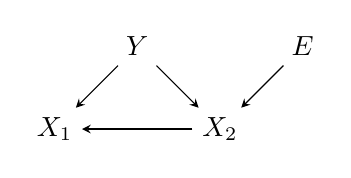
\begin{tikzpicture}[>=stealth, scale=1.05]
    \node (Y) at (0,1) {$Y$};
    \node (E) at (2,1) {$E$};
    \node (X1) at (-1,0) {$X_1$};
    \node (X2) at (1, 0) {$X_2$};
    
    \draw[->] (E) -- (X2);
    \draw[->] (Y) -- (X2);
    \draw[->] (Y) -- (X1);
    \draw[->] (X2) -- (X1);
\end{tikzpicture}
\end{minipage}\\[1pt]
where $\oplus$ is addition mod $2$, and %
%\rml{$h$ is an arbitrary function allowing each $e \in \Env$ to intervene on $X_2$.} 
the function $h(\cdot,e,\cdot)$ may vary with $e$, so that
different environments correspond to different mechanisms for $X_2$.
%
%
%
Here, $\SB(Y) = \varnothing$, and the associated DAG violates Asm.~\ref{as:A2}. There exists a classifier $f\colon \mathcal{X} \to [0,1]$ achieving a
%\rmj{uniformly lower}
Brier score risk 
that is uniformly lower than the one of
$f_{\SB(Y)} \equiv 1/2$: for all $e \in \Env$, we have
$R_e(f) \leq p(1-p) < \tfrac{1}{4} = R_e(f_{\SB(Y)})$. 
%\linus{[changed to inline]}
\end{example}
%In this example, 
Here, 
there is 
a classifier
using
$X_2 \not\in \SB(Y)$
% to adapt to the noise level in $X_1$
that 
outperforms all classifiers based on an invariant subset.
% \jonas{[to adapt to the noise level in $X_1$] could maybe also be removed?]}
%\rmj{taking $X_2 \not\in \SB(Y)$ into account allows a classifier to adapt to the noise level in $X_1$.}
%
%
%
% \rml{Ex.~\ref{ex:star_counterexample} is not an isolated case in the following sense: \eqref{eq:star} is necessary in that for any DAG in which it fails, there exists an SCM for which $f_{\SB(Y)}$ is not worst-case optimal.}
%In fact,
For regression, 
we can always construct such counterexamples:
%\rmj{$\eqref{eq:star}$ is also necessary in the sense that}
for all DAGs in which \eqref{eq:star} fails, there exists an SCM for which $f_{\SB(Y)}$ is not worst-case optimal (proved formally in Prop.~\ref{prop:star_necessary}). 
%\jonas{[move to app?]}
% \begin{proposition}
% \label{prop:star_necessary}
% Assume $\mathcal Y=\mathbb R$.
% Let $\G$ be a DAG over $(X_1,\ldots,X_d,Y,E)$ with $E$ a source node,
% no edge $E\to Y$, and let $\G_0$ be the induced subgraph on
% $(X_1,\ldots,X_d,Y)$. If \eqref{eq:star} fails, then there exists a
% set of environment $\Env$ and an SCM with graph $\G$ and induced distribution $\P$ such that
% (i) there exists $e_0\in\Env$ under which $\P_{e_0}$ is
% faithful w.r.t.\ $\G_0$,
% (ii) the second part of Asm.~\ref{as:A2} holds \felix{[make this more precise. What is the second part]} \linus{(that is, for all $e \in \Env$ there exists an environment $e' \in \Env$ for which every $j \in \CH_\mathrm{int}(Y)$ is set independently of all other variables, with all other structural assignments unchanged)}, and
% (iii) there exists a measurable $f\colon\mathcal X\to\mathbb R$ with
% $R_e(f)<R_e(f_{\SB(Y)})$ for all $e\in\Env$.
% \end{proposition}



% \begin{proposition}
% \label{prop:star_necessary}
% Assume $\mathcal Y=\mathbb R$ and $\ell(y,q)=(y-q)^2$.
% Let $\G$ be a DAG over $(X_1,\ldots,X_d,Y,E)$ with $E$ a source node,
% no edge $E\to Y$, and suppose \eqref{eq:star} fails.
% Then there exists an SCM with graph $\G$, whose induced
% distribution is Markov with respect to $\G$, such that the intervention
% part of Asm.~\ref{as:A2} holds, and there exists a measurable
% $f\colon\mathcal X\to\mathbb R$ such that for all $e \in \Env$,
% \[
% R_e(f)<R_e\bigl(f_{\SB(Y)}\bigr).
% \]
% \end{proposition}
% \begin{proposition} \label{prop:star_necessary}
% Let $\G$ be a DAG over $(X_1, \ldots, X_d, Y, E)$ with $E$ a source node, no edge $E \to Y$, and suppose \eqref{eq:star} fails. Then there exists an SCM with induced distribution $\P$ that is Markov and faithful w.r.t.\ $\G$ and a measurable $f\colon \mathcal{X} \to \mathcal{A}$ such that for all $e \in \Env$, $R_e(f) < R_e(f_{\SB(Y)}).$
% \end{proposition}

%\rml{Together, Ex.~\ref{ex:star_counterexample} and \Cref{prop:star_necessary} show that \eqref{eq:star} determines at the graph level whether worst-case optimality of $f_{\SB(Y)}$ can hold under suitable environments.}



% Having established the theoretical advantages of invariant subset classification, we turn to estimating the stable blanket from finite data without knowledge of the causal graph.

\section{
Learning subset-based predictors
} \label{sec:learning_subset_predictors}
%\subsection{Known causal graph}
When the causal graph is known, the stable blanket $\SB(Y)$ is identified and $f_{\SB(Y)}$ can be estimated by pooling data across training environments. 
%\jonas{Only the case, }
%\jonas{[habe jetzt doch mal die subsection headings entfernt]} \linus{[+1]}
%\subsection{Multiple training environments} \label{sec:mult_training_envs}
%
%
In practice, the causal graph is often unknown, and the stable blanket must be estimated using finitely many data from $\Envtr$. To do so, we can build on existing tests and methods (extending some of them to classification). To learn a predictor for $Y$, we search for subsets $S \subseteq \{1, \ldots, d\}$ that are both invariant on $\Envtr$ and predictive of $Y$. Throughout, let $\hat{f}_S: \mathcal{X} \to \mathcal{A}$ estimate $f_S(x) = \E[Y \given X_S = x_S]$, trained on data pooled across $\Envtr$; any base model (such as random forests or neural networks) can be used.
%[Directly moved paragraph on tests to appendix] 
There are various ways of testing invariance, i.e.,
%For invariance, we test the null hypothesis
$H_{0,S}\colon Y \indep E \given X_S$, %\rmj{for each $S$ (details} 
which we detail
in \Cref{app:invariance_tests}. We take the resulting
$p$-value as an invariance score $s_\mathrm{inv}(S)$, yielding
$\hat{\mathcal{I}}_{\Envtr} \coloneq \{S \given s_\mathrm{inv}(S) \geq
\alpha_\mathrm{inv} \}$ for a tuning parameter
$\alpha_\mathrm{inv} \in (0,1)$. 
%\rmj{Iterating over all $2^d$ subsets is prohibitive even for moderate $d$, so w}
We perform an optional screening
step (e.g., $\ell_1$-penalization). We denote by $s_\mathrm{pred}(S)$ a prediction score of $\hat{f}_S$, such as the out-of-sample negative MSE for regression or the out-of-sample negative binary cross-entropy for classification on the training environments.

% \jonas{[do we in the latter case not have the problem that more variables always yield better score?]} \linus{[I added "out-of-sample" also to the BCE; was meant to apply to both cases]}\jonas{+1}


\paragraph{Invariant most-predictive subsets.}
Given $\hat{\mathcal{I}}_{\Envtr}$, one option is to predict using the invariant subset with the highest prediction score, that is, $\hat{S}_\mathrm{max} \coloneq \argmax_{S \in \hat{\mathcal{I}}_{\Envtr}} s_\mathrm{pred}(S)$ \citep{rojas-carullaInvariantModelsCausal2018}. 
% \jonas{[see comment above]}
% Let $\hat{S}_\mathrm{max} \coloneq \argmax_{S \in \hat{\mathcal{I}}_{\Envtr}} s_\mathrm{pred}(S)$ be the most predictive invariant subset, and let $\hat{f}_{\hat{S}_\mathrm{max}}$ be the corresponding predictor.
%\jonas{[do you need that notation? maybe remove math here? (the formatting is a bit ugly anyways because of the vertical spacing)]}
%\rml{The resulting estimator $\hat{f}^{\mathrm{max}}(x) \coloneq \hat{f}_{\hat{S}_\mathrm{max}}\big(x_{\hat{S}_\mathrm{max}}\big)$ is sensitive to errors of the invariance test on $\hat{S}_\mathrm{max}$.} 
%\jonas{[i find the previous sentence a bit unclear. also, maybe move it into the next paragraph]} \linus{[moved to next paragraph]}
We call this approach IMP (invariant most-predictive) \citep{Gnecco2026jmlr}.
%\rml{
%Given $\hat{\mathcal{I}}_{\Envtr}$, one option is to select the invariant subset with the highest prediction score \citep{rojas-carullaInvariantModelsCausal2018}. 
% \jonas{[see comment above]}
%Let $\hat{S}_\mathrm{max} \coloneq \argmax_{S \in \hat{\mathcal{I}}_{\Envtr}} s_\mathrm{pred}(S)$ be the most predictive invariant subset, and let $\hat{f}_{\hat{S}_\mathrm{max}}$ be the corresponding predictor.
%\jonas{[do you need that notation? maybe remove math here? (the formatting is a bit ugly anyways because of the vertical spacing)]}
%\rml{The resulting estimator $\hat{f}^{\mathrm{max}}(x) \coloneq \hat{f}_{\hat{S}_\mathrm{max}}\big(x_{\hat{S}_\mathrm{max}}\big)$ is sensitive to errors of the invariance test on $\hat{S}_\mathrm{max}$.} 
%\jonas{[i find the previous sentence a bit unclear. also, maybe move it into the next paragraph]} \linus{[moved to next paragraph]}
%We call this approach IMP (invariant most-predictive) \citep{Gnecco2026jmlr}.}




\paragraph{Stabilized regression and classification.}
Since IMP is based
%relies 
on a single subset, 
%$\hat{S}_\mathrm{max}$, 
%it is sensitive to 
errors in the invariance test may have a large impact on IMP's performance.
%\jonas{[DISCUSS]}
Stabilized regression \citep{pfisterStabilizingVariableSelection2021} addresses this by using an ensemble
$\hat{f}^{\mathrm{SR}}(x) \coloneq \sum_{S \subseteq \{1, \ldots, d\}} \hat{\omega}_S \hat{f}_S(x)$, 
where the 
non-negative weights sum to one.
%\rmj{weights satisfy $\hat{\omega}_S \geq 0$ and $\sum_S \hat{\omega}_S = 1$.}
Non-zero weights are assigned only to subsets that are both invariant and sufficiently predictive, with the predictiveness threshold calibrated by a bootstrap. To the best of our knowledge, we are the first to port this idea to classification by replacing the base regressors, the prediction score (cross-entropy instead of MSE), and the invariance tests with their classification counterparts, yielding stabilized classification (SC). Details on SC are given in \Cref{app:SC_alg}.



\section{Experiments} \label{sec:experiments}
\subsection{Synthetic prediction-intervention games}
\label{sec:synthetic_experiments}

We validate our theoretical results for prediction-intervention games on synthetic data.
For this we consider two data-generating processes: 
a linear-Gaussian SCM and a nonlinear SCM. %
Both have the same induced graph depicted 
in \cref{fig:synthetic_dag}.
The causal parents of $Y$ are equal to
\begin{wrapfigure}[13]{r}{0.5\textwidth}
    \centering
    \vspace{-0.15cm}
    \begin{tikzpicture}[
        >=Stealth,yscale=0.99,xscale=0.7,
        var/.style={draw, circle, minimum size=7mm, inner sep=1pt, font=\small},
        pa/.style={var, fill=softsage},
sbadd/.style={var, fill=softrose},
        env/.style={draw, rectangle, rounded corners, minimum width=7mm, minimum height=7mm, inner sep=2pt, font=\small},
        arr/.style={->, thick},
        intarr/.style={->, thick, dashed}
    ]
        % Nodes
        \node[pa]    (X2) at (-1.0,0.0) {$X_2$};
        \node[pa]    (X1) at (-1.0,2.0) {$X_1$};
        \node[var]   (Y)  at (1.,1.0) {$Y$};
        \node[sbadd] (X3) at (2.5,1.0) {$X_3$};
        \node[var]   (X4) at (2.5,0.0) {$X_4$};
        \node[var]   (X5) at (4.5,0.0) {$X_5$};
        \node[env]   (E)  at (4.5,2.0) {$E$};

        % Structural edges
        \draw[arr] (X2) -- (X1);
        \draw[arr] (X1) -- (Y);
        \draw[arr] (X2) -- (Y);
        \draw[arr] (Y) -- (X3);
        \draw[arr] (Y) -- (X4);
        \draw[arr] (X2) -- (X4);
        \draw[arr] (X4) -- (X5);

        % Intervention edges
        \draw[intarr] (E) -- (X1);
        \draw[intarr] (E) -- (X4);
    \end{tikzpicture}
%    \vspace{-0.5\baselineskip}
    \caption{DAG in \Cref{sec:synthetic_experiments}. %Here, 
    $\PA(Y)=\{X_1,X_2\}$ (blue),  
    $\SB(Y)=\{X_1,X_2,X_3\}$ (blue and red). 
    %The all-variable predictor
    %uses $\{X_1,X_2,X_3,X_4,X_5\}$. 
    %Dashed arrows from $E$ indicate the direct
    %intervention targets $X_1$ and $X_4$. 
    $\SB(Y)$ contains the
    non-intervened child $X_3$, but not the intervened child $X_4$ and its
    descendant $X_5$.}
    \label{fig:synthetic_dag}
    %\vspace{-2.5em}
\end{wrapfigure}
 $\PA(Y)=\{X_1,X_2\}$, while the stable blanket is
$\SB(Y)=\{X_1,X_2,X_3\}$. The follower may intervene on $X_1$ and on $X_4$.
We compare three predictors (either in a population or finite-sample version): 
%the population and the fitted 
based on $\PA(Y)$,
$\SB(Y)$, or all variables.
The follower is represented by a neural intervention mechanism with intervention
bound $b$ and is trained either to maximize the leader's MSE or to minimize the
prediction value (for details see \Cref{sec:sdfds}). All results are averaged over 10 independent runs, with shaded regions indicating $95\%$ confidence intervals for the mean. Further details on the setup are provided in \Cref{app:dgp}.
%
%\begin{figure}[t]
% \begin{figure}[t]
%     \centering
%     \begin{minipage}[c]{0.5\linewidth}
%         \centering
%         \begin{tikzpicture}[
%             >=Stealth,
%             var/.style={draw, circle, minimum size=7mm, inner sep=1pt, font=\small},
%             pa/.style={var, fill=softsage},
%             sbadd/.style={var, fill=softrose},
%             env/.style={draw, rectangle, rounded corners, minimum width=7mm,
%                         minimum height=7mm, inner sep=2pt, font=\small},
%             arr/.style={->, thick},
%             intarr/.style={->, thick, dashed}
%         ]
%             \node[pa]    (X2) at (-1.0,0.0) {$X_2$};
%             \node[pa]    (X1) at (-1.0,2.0) {$X_1$};
%             \node[var]   (Y)  at (1.,1.0)   {$Y$};
%             \node[sbadd] (X3) at (2.5,1.0)  {$X_3$};
%             \node[var]   (X4) at (2.5,0.0)  {$X_4$};
%             \node[var]   (X5) at (4.5,0.0)  {$X_5$};
%             \node[env]   (E)  at (4.5,2.0)  {$E$};
%             \draw[arr]    (X2) -- (X1);
%             \draw[arr]    (X1) -- (Y);
%             \draw[arr]    (X2) -- (Y);
%             \draw[arr]    (Y)  -- (X3);
%             \draw[arr]    (Y)  -- (X4);
%             \draw[arr]    (X2) -- (X4);
%             \draw[arr]    (X4) -- (X5);
%             \draw[intarr] (E)  -- (X1);
%             \draw[intarr] (E)  -- (X4);
%         \end{tikzpicture}
%     \end{minipage}%
%     \hfill
%     \begin{minipage}[c]{0.46\linewidth}
%         \captionof{figure}{Synthetic SCM used in the experiments. The parent
%         set is $\PA(Y)=\{X_1,X_2\}$ (blue nodes), while the stable blanket is
%         $\SB(Y)=\{X_1,X_2,X_3\}$ (blue and red nodes). The all-variable
%         predictor uses $\{X_1,X_2,X_3,X_4,X_5\}$. Dashed arrows from $E$
%         indicate the direct intervention targets $X_1$ and $X_4$. The stable
%         blanket includes the non-intervened child $X_3$, but excludes the
%         intervened child $X_4$ and its descendant $X_5$.}
%         \label{fig:synthetic_dag}
%     \end{minipage}
% \end{figure}

We first consider the linear-Gaussian SCM (\Cref{fig:synthetic_main}, left). In this setting the relevant conditional
expectations are available in closed form, so the predictors use population
regression quantities rather than estimates from finite training data. This
isolates the effect of the follower's intervention from statistical estimation
errors. As predicted by our theory in \cref{sec:parents}, both $\PA(Y)$ and $\SB(Y)$ yield
constant deployment MSE. $\SB(Y)$ improves over $\PA(Y)$ because the non-intervened child $X_3$ carries additional stable
information about $Y$. By contrast, the all-variable predictor is highly
unstable: it performs well for weak interventions, but its MSE increases sharply
as the intervention bound grows, since it relies on the manipulable variable $X_4$.
%s
%\rml{$X_4$ and $X_5$} \linus{$X_1$ and $X_4$ [typo?]}. \jonas{[4 and ]}

The nonlinear SCM shows the same qualitative ordering (\Cref{fig:synthetic_main}, right). The stable blanket and
the parent set remain much more stable than the all-variable predictor, and the
stable blanket again improves over the parents. Unlike in the linear-Gaussian
experiment, however, the stable-blanket and parent predictors are not perfectly
flat. This is because the nonlinear predictors are learned from finite training
data. The follower can exploit finite-sample regression errors by shifting the
test distribution toward regions in which the fitted predictor differs from the
population regression function. \Cref{app:synthetic_regression_error}
investigates this effect directly: as the leader's training sample size grows,
the MSE curves for $\PA(Y)$ and $\SB(Y)$ become more stable, while the
all-variable predictor remains unstable.

Finally, we also allow the follower's intervention on $X_4$ to depend on
$X_1$ and $X_3$ in addition to its usual inputs. The qualitative results do not
change; see \Cref{app:synthetic_details}. This is consistent with the
graphical theory from \Cref{sec:augmentation}: adding these action-parent edges does not change the stable
blanket.
\individualexp{\Cref{app:individual_followers} presents a similar experiment with individual followers as in \Cref{sec:individuals} instead of the follower used here; the leader's deployment MSE is nearly the same.}
%\rml{, so the same invariant set remains the robust choice}.

\begin{figure*}[t]
    \centering
    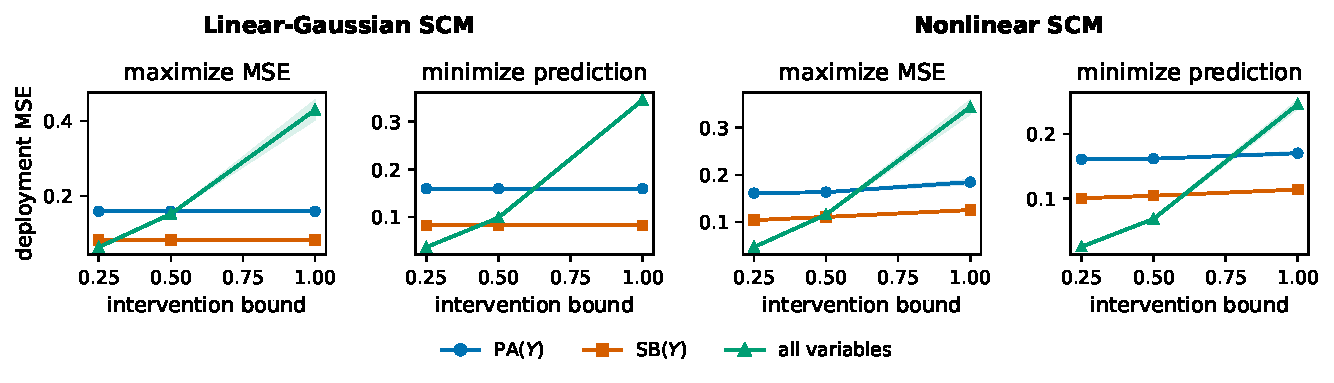
\includegraphics[width=\textwidth]{images/lineargaussian_standard_row_grouped.pdf}
    \caption{Synthetic prediction-intervention games. Left two panels:
    linear-Gaussian SCM with population regression predictors. Right two panels:
    nonlinear SCM with predictors estimated from finite data. The stable blanket
    is uniformly better than the parent set and both are substantially more
    stable than the all-variable predictor. In the nonlinear SCM, small
    deviations from perfectly constant MSE are due to finite-sample regression
    error.}
    \label{fig:synthetic_main}
\end{figure*}


\subsection{Prediction-intervention games on Causal Chambers} \label{sec:new_chamber_experiments}
We complement the synthetic experiments of \Cref{sec:synthetic_experiments} with a prediction-intervention game on real data from the Causal Chambers\footnote{The Causal Chambers are devices controlled through an API and collect measurements from a physical system with known causal ground truth.} light tunnel (\cref{fig:causal_chambers_dags} left) of \citet{gamellaCausalChambersRealworld2025}.


\paragraph{Setup.} 
The chamber takes a light source setting $\mathtt{RGB} \coloneq (\mathtt{red}, \mathtt{green}, \mathtt{blue}) \in \mathbb{R}^3$ and returns infrared and visible-light measurements ($\mathtt{ir\_j}$, $\mathtt{vis\_j}$) at positions $\mathtt{j} \in \{1,2,3\}$ along the chamber.
We aim to predict $Y \in \{0,1\}$ (constructed %\rml{which we construct}
as a function of $\mathtt{ir\_1}$) 
and observe the system under different environments. 
The leader's loss is the MSE; the follower's objective is to minimize the population mean prediction $\Vfoll_e(\hat{f}) = -\E_e[\hat{f}(X)]$, as considered in \Cref{thm:PA_vs_SB_game}.
Given $\hat{f}$, the follower can query the Causal Chambers API to receive $500$ observations of $X$ under different interventions on $\mathtt{ir\_3}$ and $\mathtt{vis\_3}$. We consider a fixed collection of $49$ candidate environments the follower can choose from. We restrict their choice with an intervention bound $b \in [0, 1]$: only the $\max\{1,\lceil 49b \rceil \}$
environments closest to a reference environment $e_\mathrm{ref}$ are available.
%\rml{, growing monotonically from $\{e_\mathrm{ref}\}$ at $s=0$ to all $49$ environments at $s=1$}. 
All details can be found in \Cref{app:additional_details_causal_chambers}.


\begin{figure}[t]
    \centering
    \begin{minipage}{0.25\textwidth}
        \centering
        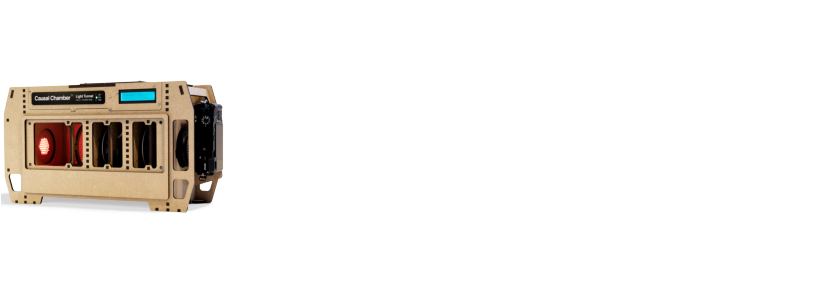
\includegraphics[width=\linewidth]{images/causal_chamber.pdf}
    \end{minipage}
    \hfill
    \begin{minipage}{0.35\textwidth}
        \centering
        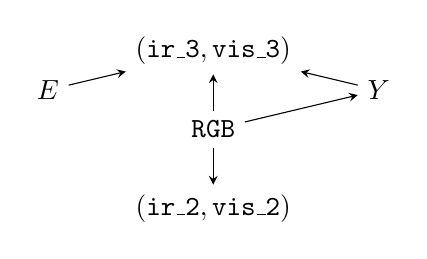
\begin{tikzpicture}[>=stealth, scale=1.0]
    \node (E) at (-2.1, 0.5) {$E$};
    \node (RGB) at (0, 0) {$\mathtt{RGB}$};
    \node (Y) at (2.1, 0.5) {$Y$};
    \node (Bottom) at (0, -1) {$(\mathtt{ir\_2}, \mathtt{vis\_2})$};
    \node (Top) at (0, 1) {$\mathtt{(ir\_3, vis\_3)}$};
    % \node (ir2) at (-0.8, -0.8) {$\mathtt{ir\_2}$};
    % \node (vis2) at (0.8, -0.8) {$\mathtt{vis\_2}$};

    \draw[->] (E) -- (Top);
    % \draw[->] (E) -- (RGB);
    \draw[->] (RGB) -- (Top);
    \draw[->] (RGB) -- (Y);
    \draw[->] (Y) -- (Top);
    \draw[->] (RGB) -- (Bottom);
    %\draw[->] (RGB) -- (vis2);
\end{tikzpicture}
    \end{minipage} \hfill
    \begin{minipage}{0.35\textwidth}
        \centering
        % \begin{tikzpicture}[>={Stealth[round]}, scale=0.7, 
%     every node/.style={draw, ellipse, minimum height=0.96cm, align=center}]
    
%     % The central RGB node
%     \node (rgb) at (0, 0) {$\mathtt{red, green, blue}$};
    
%     % The top combined node
%     \node (ir3vis3) at (0, 3.0) {$\mathtt{ir\_3, vis\_3}$};
    
%     % Similarly align ir_1 and vis_1
%     \node (ir1) at (rgb.west |- 0, -2.0) [anchor=west] {$\mathtt{ir\_2}$};
%     \node (vis1) at (rgb.east |- 0, -2.0) [anchor=east] {$\mathtt{vis\_2}$};
    
%     % Y and E nodes at y=2.0
%     % Positioned vertically halfway, horizontally aligning with the outer edges of the red, green, blue box
%     \node[circle, fill=gray!50, minimum size=0.96cm, inner sep=0pt] (Y) at (rgb.west |- 0, 1.5) {$Y$};
%     \node[circle, fill=gray!50, minimum size=0.96cm, inner sep=0pt] (E) at (rgb.east |- 0, 1.5) {$E$};

%     % Edges mapping according to sketch
%     \draw[->] (rgb) -- (ir1);
%     \draw[->] (rgb) -- (vis1);
    
%     \draw[->] (rgb) -- (Y);             % rgb up-left to Y
%     \draw[->] (Y) -- (ir3vis3.200);     % Y up-right to top node
    
%     \draw[->] (rgb) -- (ir3vis3);       % rgb straight up to top node
    
%     \draw[->] (E) -- (rgb.20);          % E down-left to rgb (tweaking angle for spacing)
%     \draw[->] (E) -- (ir3vis3.340);     % E up-left to top node

% \end{tikzpicture}

% \begin{tikzpicture}[>=stealth, scale=1.0]
%     \node (E) at (-2.1, 0.5) {$E$};
%     \node (RGB) at (0, 0) {$\mathtt{(red, green, blue)}$};
%     \node (Y) at (2.1, 0.5) {$Y$};

%     \node (Top) at (0, 1) {$\mathtt{(ir\_3, vis\_3)}$};
%     \node (ir2) at (-0.8, -0.8) {$\mathtt{ir\_2}$};
%     \node (vis2) at (0.8, -0.8) {$\mathtt{vis\_2}$};

%     \draw[->] (E) -- (Top);
%     \draw[->] (E) -- (RGB);
%     \draw[->] (RGB) -- (Top);
%     \draw[->] (RGB) -- (Y);
%     \draw[->] (Y) -- (Top);
%     \draw[->] (RGB) -- (ir2);
%     \draw[->] (RGB) -- (vis2);
% \end{tikzpicture}

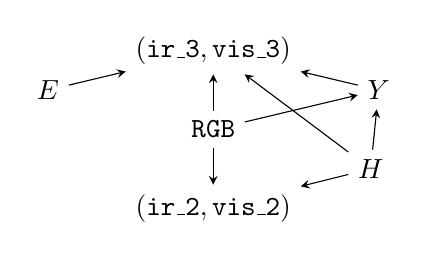
\begin{tikzpicture}[>=stealth, scale=1.0]
    \node (E) at (-2.1, 0.5) {$E$};
    \node (RGB) at (0, 0) {$\mathtt{RGB}$};
    \node (Y) at (2.1, 0.5) {$Y$};
    \node (H) at (2, -0.5) {$H$};
    \node (Bottom) at (0, -1) {$(\mathtt{ir\_2}, \mathtt{vis\_2})$};
    \node (Top) at (0, 1) {$\mathtt{(ir\_3, vis\_3)}$};

    \draw[->] (E) -- (Top);
    \draw[->] (RGB) -- (Top);
    \draw[->] (RGB) -- (Y);
    \draw[->] (Y) -- (Top);
    \draw[->] (RGB) -- (Bottom);
    \draw[->] (H) -- (Top);
    \draw[->] (H) -- (Bottom);
    \draw[->] (H) -- (Y);
\end{tikzpicture}
    \end{minipage}
    \caption{
    %\linus{[TODO: make DAGs prettier]} 
    Left: light tunnel 
    %\rmj{hardware} 
    (adapted from \citet{gamellaCausalChambersRealworld2025}, licensed under CC BY 4.0).
    %and causal graph restricted to the variables used in our experiment ($\mathtt{ir\_3}$ and $\mathtt{vis\_3}$ are grouped as they share the same parents). 
    Middle: inaccurate graph, 
    inferred from the partial causal-graph information by
    %\jonas{the partial knowledge graph in [pls check with Juan -- we probably write in his paper somewhere that there is hidden confounding on top of everything]}
    \citet{gamellaCausalChambersRealworld2025}; 
    the follower is allowed to intervene on 
    %with edges from $E$ to 
    $\mathtt{ir\_3}, \mathtt{vis\_3}$;
    %added to reflect our interventions; 
    the stable blanket of $Y$ is $\{\mathtt{RGB}\}$. Right: potentially correct graph with a hypothesized hidden confounder $H$ pointing to all $\mathtt{ir\_j}$ and $\mathtt{vis\_j}$; the stable blanket of $Y$ is $\{\mathtt{RGB}, \mathtt{ir\_2}, \mathtt{vis\_2}\}$.}
    \label{fig:causal_chambers_dags}
\end{figure}


 
\paragraph{Inaccurate causal graph.}
\citet{gamellaCausalChambersRealworld2025} provide partial causal-graph
information for the light tunnel. 
They note that absent edges do not necessarily exclude the existence of
causal effects or hidden confounding.
% \jonas{A careless reader 
% ignoring this note and adding the edges from $Y$ and $E$ to
% $(\mathtt{ir\_3}, \mathtt{vis\_3})$ may consider the graph in \cref{fig:causal_chambers_dags} (middle) as ground truth.} \linus{[I implemented the first part of your suggestion. Regarding the remaining part: I think the way we write the "story" here (first we have the wrong DAG, then the hypothesis, then the better DAG) I think we are implicitly saying we are that "careless reader" :-) Maybe a bit less negative:]}
% \jonas{+1!}
% %
Ignoring this note and adding the edges from $Y$ and $E$ to
$(\mathtt{ir\_3}, \mathtt{vis\_3})$, one might be tempted to consider the graph in \cref{fig:causal_chambers_dags} (middle) as ground truth.
% \jonas{+1}
% \rml{Taking the ground-truth causal graph provided by \citet{gamellaCausalChambersRealworld2025}
% %\jonas{[provide precise ref]}\linus{[do we have to say smt like ``see the website in the comment in the bibliography''?]} 
%  and adding the edges from $Y$ and $E$ to $(\mathtt{ir\_3}, \mathtt{vis\_3})$, we obtain the graph shown in \cref{fig:causal_chambers_dags} (middle).} 
%The stable blanket of $Y$ is $\{\mathtt{RGB}\}$. 
However, 
there is empirical evidence that this
is not the correct graph for our experiment:
conditional independence tests on training data reject\footnote{Specifically, $\mathtt{ir\_i} \indep \mathtt{ir\_j} \given \mathtt{RGB}$ and $\mathtt{vis\_i} \indep \mathtt{vis\_j} \given \mathtt{RGB}$ for $\mathtt{i} \ne \mathtt{j} \in \{1, 2, 3\}$ are rejected in the majority of training environments at level $0.01$; see \Cref{app:hidden_confounding}.} some of the implied independencies between sensors. %measurements implied by this graph.
We
hypothesize that this is due to a hidden confounder (such as background
lighting) acting on the sensors. Adding it results in \cref{fig:causal_chambers_dags} (right). Under this extended graph with hidden variables the stable blanket of $Y$
can be defined analogously \citep{xiangStableBlanketHidden2026} and
equals $\{\mathtt{RGB}, \mathtt{ir\_2}, \mathtt{vis\_2}\}$. 
%The correct graph is therefore unclear; the leader can fit a predictor on a chosen covariate subset, or use stabilized classification (\Cref{sec:learning_subset_predictors}), which does not require graph knowledge.

%\paragraph{Setup.}

%The leader's loss is the MSE. The follower's objective is to minimize the population mean prediction $\Vfoll_e(\hat{f}) = -\E_e[\hat{f}(X)]$, a setting considered in \Cref{thm:PA_vs_SB_game}.
%Given $\hat{f}$, the follower can query the Causal Chambers API to receive $500$ observations of $X$ under different interventions on $\mathtt{ir\_3}$ and $\mathtt{vis\_3}$. We consider a fixed collection of $49$ candidate environments the follower can choose from. We restrict its choice with an intervention bound $s \in [0, 1]$: only the $\lceil 49 s \rceil$ environments closest to a reference environment $e_\mathrm{ref}$ are available, growing monotonically from $\{e_\mathrm{ref}\}$ at $s=0$ to all $49$ environments at $s=1$. 
%We report the resulting shift in the population mean prediction (that is, the degree to which the follower can improve its objective) and the leader's MSE under the chosen environment, both computed on $500$ new evaluation observations. Details are in Appendix~XY.


 

 
\begin{figure}[t]
    \centering
    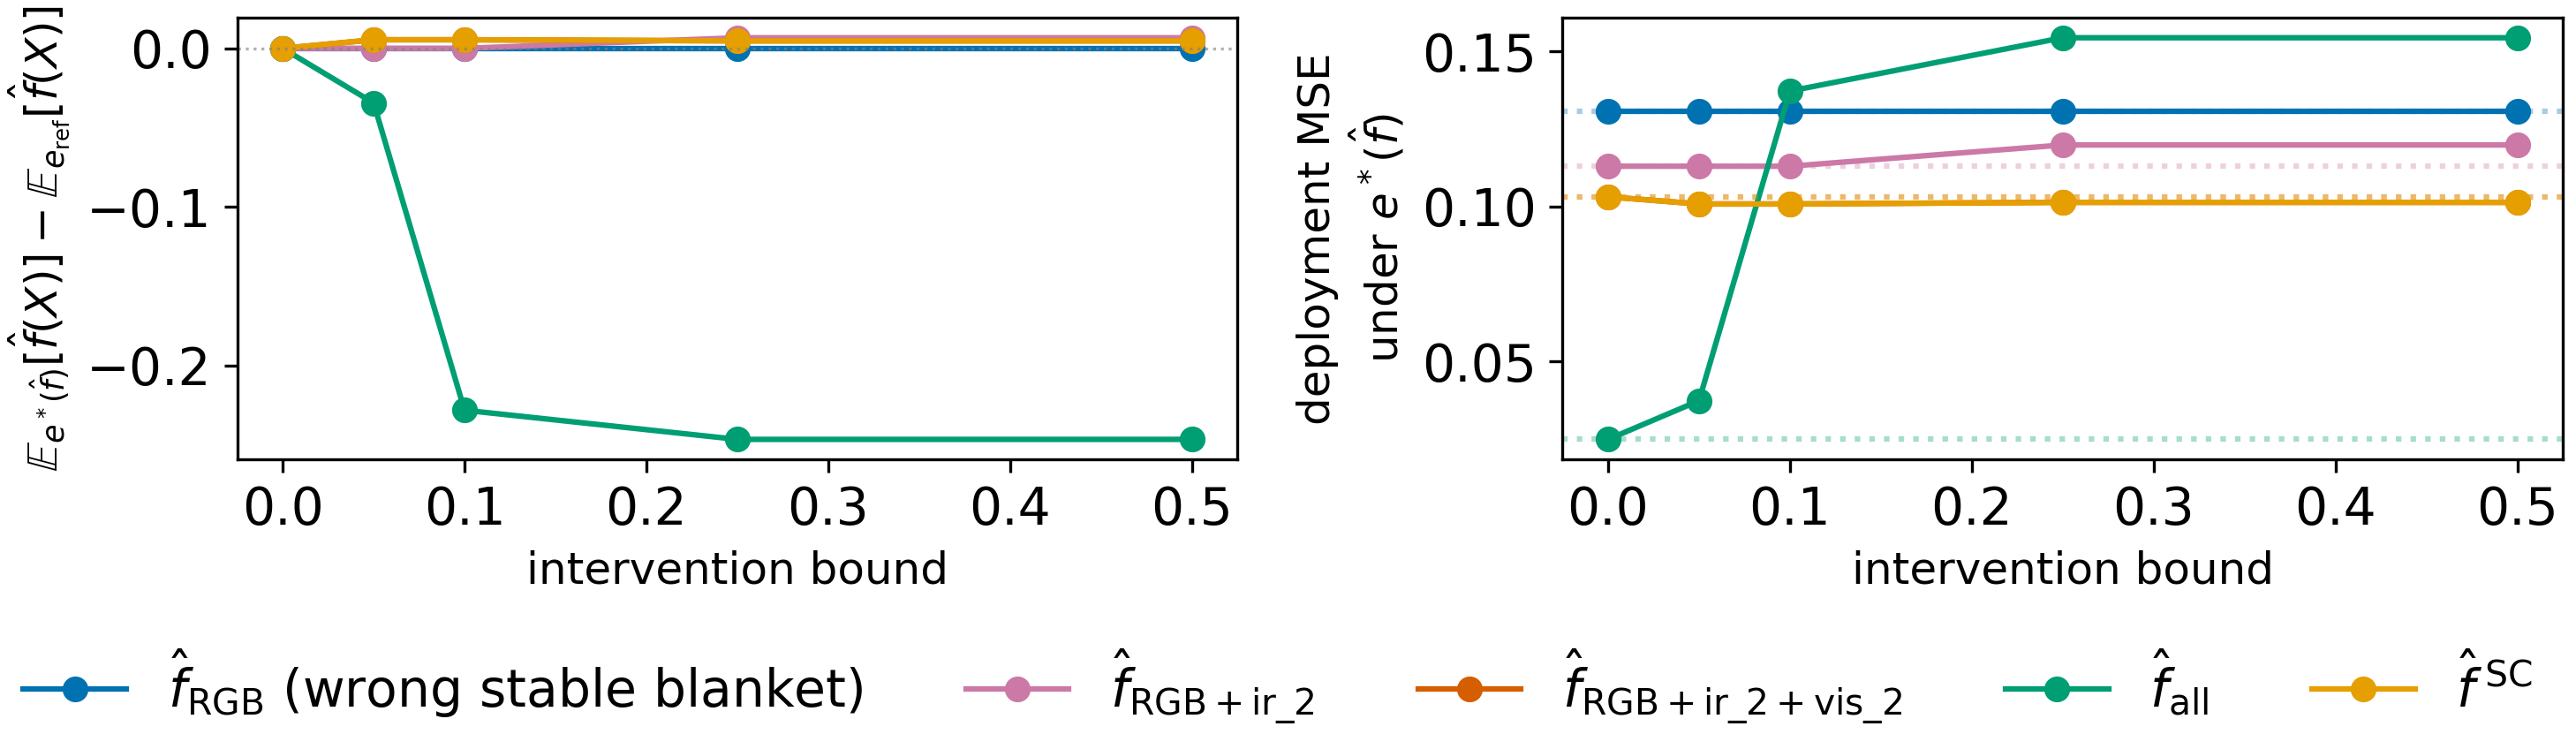
\includegraphics[width=1\linewidth]{images/causal_chambers_game.png}
    \caption{%
        Prediction-intervention game on Causal Chambers data (\Cref{sec:new_chamber_experiments}). %, with increasing intervention options for the follower. 
        Follower-induced shift in the population mean prediction relative to a reference environment $e_\mathrm{ref}$ (left) and
%        %$\E_{e^*(\hat{f})}[\hat{f}(X)] - \E_{e_\mathrm{ref}}[\hat{f}(X)]$
        MSE of the leader's deployed predictor %$R_{e^*(\hat{f})}(\hat{f})$
        in the follower's chosen environment (right).
        %\rml{, both relative to a reference environment $e_\mathrm{ref}$}.
%        ; dotted lines mark the MSE
 %       in $e_\mathrm{ref}$. 
 The follower has a strong influence on their objective only for $\hat{f}_\text{all}$.
 %, increasing its MSE; the other four predictors are essentially unaffected. 
% $\hat{f}_{\mathtt{RGB}, \mathtt{ir\_2}, \mathtt{vis\_2}}$ and 
$\hat{f}^\mathrm{SC}$ achieves the lowest MSE under the follower's chosen environment, tied with $\hat{f}_{\mathtt{RGB}, \mathtt{ir\_2}, \mathtt{vis\_2}}$
(curves overlap); 
it does not require graph knowledge and can thus not be deceived by wrong assumptions. 
% \linus{[to myself: new plot]} \jonas{[for me, either version works (with the large sample size, pls mention that red and yellow are on top of each other; with the small sample size, pls mention the downsampling)]}
}
    \label{fig:follower_chambers}
\end{figure}
 
\paragraph{Results.}
\cref{fig:follower_chambers} 
%shows the results. 
shows 
the degree to which the follower can improve their objective (left), and the leader's MSE under the environment chosen by the follower (right), both computed on $500$ new evaluation observations.
%as the set of available environments increases, the follower lowers the mean prediction of $\hat{f}_\mathrm{all}$ by around $0.25$ relative to $e_\mathrm{ref}$ (all predictors output values in $[0,1]$). 
%[still need to update this bit]
Only under $\hat{f}_\text{all}$ (using all variables) can the follower improve their objective (left), and for large intervention bounds, this predictor performs worst for the leader. 
%
%Given the four remaining predictors, the follower is not able to meaningfully change the mean predictions, and the leader's risk stays essentially constant. Among them, 
$\hat{f}_{\mathtt{RGB}}$ is the stable blanket predictor under the inaccurate graph and 
has a higher MSE than the larger subsets that include $\mathtt{ir\_2}$ and $\mathtt{vis\_2}$ on the reference environment. This is consistent with the hidden-confounding hypothesis that the graph is incorrect. 
%The MSE of $\hat{f}^\mathrm{SC}$ closely aligns with that of $\hat{f}_{\mathtt{RGB}, \mathtt{ir\_2}, \mathtt{vis\_2}}$ (the stable blanket under the hidden-confounder graph).
The SC predictor $\hat{f}^\mathrm{SC}$, which is purely based on data, selects $\{\mathtt{RGB}, \mathtt{ir\_2}, \mathtt{vis\_2}\}$ (the stable blanket under the hidden-confounder graph) as the unique subset passing both the
invariance and predictiveness filters, and therefore matches the performance
of $\hat{f}_{\mathtt{RGB}, \mathtt{ir\_2}, \mathtt{vis\_2}}$; thus, $\hat{f}^\mathrm{SC}$ cannot be deceived
by inaccurate assumptions on the causal graph. 

%The MSE of $\hat{f}_\mathrm{all}$ starts as the lowest of the five but exceeds the others once $s \ge 0.1$ on the environment chosen by the follower. Given the four remaining predictors, the follower is not able to meaningfully change the mean predictions, and the leader's risk stays essentially constant. Among them, $\hat{f}_{\mathtt{RGB}}$ (the stable blanket under the documented graph) has a higher MSE than the larger subsets that include $\mathtt{ir\_2}$ and $\mathtt{vis\_2}$ on the reference environment, consistent with the hypothesis that the documented graph is incorrect. The MSE of $\hat{f}^\mathrm{SC}$ closely aligns with that of $\hat{f}_{\mathtt{RGB}, \mathtt{ir\_2}, \mathtt{vis\_2}}$ (the stable blanket under the hidden-confounder graph).












\section{Discussion and future work} \label{sec:conclusion}
%TODO (Summary, limitations, future work)
%\linus{[HAS to quickly mention limitations (checklist)]}

% We have introduced
% prediction-intervention games,  have connected them 
% to invariant sets and worst-case distribution generalization and have proved optimality results for strategies based on the stable blanket. 
% %We 
% %It might 
% %a setting that  
% Our current results are limited by the assumption of strong interventions.
% %and by the fact the bound in~\eqref{} is not tight. 
% %We also think that the finite sample results should be understood better (see \Cref{}).
% {\color{red}We think that analyzing the game's value and optimal strategies
% under alternative (such as weaker interventions) 
% or more general conditions  is an interesting task for future research.}
% We hypothesize that 
% solving prediction-intervention games is in general a hard problem \citep[e.g.,][]{ConitzerS06}.
% Finally, we aim for a more refined analysis of the effect of estimation errors (\Cref{app:synthetic_regression_error}). 
% %Analyzing the game's value and optimal strategies
% %under general conditions and the feasibility of computing those is interesting future research.



% The worst-case optimality of the stable blanket heavily relies on 'strong interventions' assumptions (A1 and A2), which may be unrealistic in practical prediction-intervention games where followers face high costs and possess bounded manipulation capabilities. Under restricted bounded shifts, alternative function-based predictors like anchor regression might be preferable.

 % The upper bound in Equation 3 reduces the problem to distribution generalization, which assumes the worst-case intervention will occur regardless of the follower's actual incentives. This relaxation can lead to overly conservative and suboptimal leader strategies when the follower's true utility function restricts them to a narrow, predictable set of interventions.




We have introduced prediction-intervention games, connected them to
invariant sets and worst-case distribution generalization, and proved
optimality results for strategies based on the stable blanket. We proposed learning methods that the leader may use for settings in which the causal graph is known and settings in which it is not, and have successfully tested them on data.
One limitation of our results is that they
%Our current results 
rely on the assumption of strong interventions;
analyzing optimal strategies under weaker or
more general conditions is an interesting direction for future research.
We hypothesize that solving prediction-intervention games is in
general a hard problem \citep[e.g.,][]{ConitzerS06}.
% Two extensions of the follower model seem worthwhile.
% First, considering
% a population of heterogeneous followers with different objectives would
% induce a mixture over best-responses rather than a single $e^*(f)$.
Extending the follower model also seems worthwhile, for example by
adding constraints on the allowed interventions or
considering a population of heterogeneous followers with different
objectives.
Finally, in practice, the leader uses a finite-sample estimate $\hat f_S$ rather than
the population predictor $f_S$, and the follower can shift covariates to high-error regions
(\Cref{app:synthetic_regression_error}); a finite-sample analysis is left for future work.





\begin{ack}
We thank Niklas Pfister and Sorawit Saengkyongam for helpful discussions, and Juan Gamella for the help with the Causal Chambers data generation. During this work, LK was
%\rmj{primarily} \linus{[is this a strong opinion? This is exactly what the ai center wants me to write]}\jonas{[yes -- costs are split 50/50, so ``primarily'' is incorrect -- any complaints you can forward to me :).]}
supported by the ETH AI Center through an ETH AI Center doctoral fellowship. \linus{[add anon reviewers]}
\end{ack}


\linus{[Jonas: why change the Xiang Stable blanket with hidden variables and cycles citation?]}

\vskip 0.2in
\bibliographystyle{plainnat}
\bibliography{references}

\appendix
\clearpage

\addcontentsline{toc}{section}{Appendix}

\listofappendices
\vskip 0.75in


\appsection{Extended related work} \label{app:extended_related_works}




We expand on the related work discussion from \Cref{sec:intro}.
 
\paragraph{Strategic classification and performative prediction.}
Strategic classification \citep{brucknerStackelbergGamesAdversarial2011, hardtStrategicClassification2016} models followers who respond to a deployed classifier $f$ by modifying their features with some cost $c$ to obtain a more favorable prediction, typically through the pointwise best response $x^f \in \argmax_{x'} f(x') - c(x, x')$. The leader's goal is to learn an $f$ that is robust under the induced distribution shift. The leader's and follower's objectives are typically asymmetric in this Stackelberg formulation; \citet{ehrenbergAdversariesIncentivesStrategic2024} make this explicit and study a game in which the leader minimizes a worst-case loss over a set of different utility-maximizing opponents, without a causal structure over $X$ and $Y$. A related question is how the choice of predictor creates different incentives for the followers and distinguishes gaming the system 
%\jonas{[also, maybe add a sentence how they define gaming wout the notion of an SCM]}
from genuine improvement:
% \rml{, see for example \citet{kleinbergHowClassifiersInduce2019, chenLinearClassifiersThat2021}.}
\citet{kleinbergHowClassifiersInduce2019} model followers as investing effort into different actions that affect the observed features, and ask which decision rules incentivize followers to invest in actions a leader views as valuable rather than in gaming; \citet{chenLinearClassifiersThat2021} distinguish improvable, manipulable, and immutable features, with gaming defined as changes to manipulable features that by assumption do not affect $Y$. They do not specify a full SCM over $(X, Y, E)$ that determines how the follower's actions propagate through the whole system. Performative prediction \citep{perdomo2020performative, hardtPerformativePredictionFuture2025} considers the broader phenomenon that deployed models shift the data distribution; \citet{mendler-dunnerAnticipatingPerformativityPredicting2022} address identifiability of the causal effect of predictions. These works do not generally specify the follower's moves through an SCM.
%\linus{More broadly, the prediction-intervention game~\eqref{eq:pred_intervention_game} is a bilevel optimization problem \citep{zhangIntroductionBilevelOptimization2024}, \jonas{[move up and state hardness?]} and other game-theoretic interactions between predictors and strategic agents have been studied in market settings \citep{huIncentivizingHighQualityContent2023}.}
Other game-theoretic interactions between predictors and strategic agents have been studied in market settings \citep{huIncentivizingHighQualityContent2023}.
% \jonas{+1}



\paragraph{Causal Stackelberg formulations.}
% \jonas{[I think this paragraph would benefit from a rewrite. try to be extra clear on what we do what they do not (if applicable :-)) -- ideally, for each reference]}
Several works model Stackelberg games with SCMs. 
% \rml{\citet{shavitCausalStrategicLinear2022} formulate strategic linear regression with an intervention set constrained by an SCM. \citet{miller2020strategic} argue that designing classifiers that incentivize improvement essentially solves a causal-discovery problem. \citet{yanDiscoveringOptimalScoring2023} study optimal scoring mechanisms when the causal graph is unknown. Closest to our setting is \citet{horowitzCausalStrategicClassification2023}, who partition covariates into causal and noncausal predictive components. Their follower is an individual who modifies covariates to change the prediction in its favor, and only changes to causal variables propagate to $Y$. Our formulation allows us to model the follower flexibly: we specify which variables they may intervene on, and which other variables their interventions may depend on. The latter can induce additional edges in the graph, so our setup accommodates settings in which the deployment graph extends the training graph. \citet{kulynychCausalPredictionCan2022} includes the deployed predictor in the causal graph as a node and studies under which conditions the Markov blanket is optimal.}
\citet{shavitCausalStrategicLinear2022} formulate strategic linear regression in a linear SCM, and learn linear predictors targeting one of three specific objectives: minimizing the leader's risk under strategic follower responses, incentivizing followers to genuinely improve their outcomes, or estimating the parameters of the outcome model. Their algorithms deploy multiple predictors and observe the resulting follower responses to learn the final predictor. In contrast, our predictor is defined without observing follower interventions. We further allow a general SCM, cover regression and classification under any loss strictly consistent for the mean functional, and place no specific functional form on the follower's response: their setup fixes it through an effort conversion matrix and a quadratic cost, whereas ours constrains the follower only through the graph $\G$ and the action sets $A_j$.
\citet{miller2020strategic} develop a causal framework that distinguishes gaming from improvement and prove that designing classifiers which incentivize improvement is at least as hard as orienting the edges of the underlying causal graph. Their contribution is conceptual and concerns the difficulty of incentive design, while we focus on the leader's optimal choice of $f$ given an SCM.
\citet{yanDiscoveringOptimalScoring2023} assume an unknown causal graph and follower manipulations constrained by a fixed budget. Their algorithm iteratively deploys predictors and observes strategic responses to recover the graph, and their leader objective trades off prediction accuracy with outcome improvement. Our predictor does not require iterated deployment, and in the unknown-graph case (\Cref{sec:learning_subset_predictors}) we use multiple training environments instead of observed strategic responses.
\citet{horowitzCausalStrategicClassification2023} partition covariates into causal and non-causal predictive components. Their follower is an individual who modifies covariates to change the prediction in its favor, and only changes to causal variables propagate to $Y$. 
%Our formulation allows 
We, instead, allow for a more flexible model of the follower:  we may specify which variables the follower may intervene on, and which other variables their interventions may depend on. The latter can induce additional edges in the graph, so our setup accommodates settings in which the deployment graph extends the training graph. Unlike the work by \citet{horowitzCausalStrategicClassification2023}, we do not estimate the causal function of the response but work with invariant sets; furthermore, we admit regression in addition to classification, allow for more general losses 
and for more general follower utilities; finally, \citet{horowitzCausalStrategicClassification2023} do not provide optimality results in their setting.
\citet{kulynychCausalPredictionCan2022} extends an SCM over $(X,Y)$ by including the deployed predictor as an additional node $M$, with edges $M \to X$ but no edge to $Y$. Instead of modeling a follower optimizing its own utility, the deployment-induced shift in $X$ is encoded directly in the structural assignments of the SCM. In this setting, they study conditions under which the Markov-blanket predictor remains optimal under the shift it induces. In our formulation, the post-deployment distribution instead arises from a follower choosing interventions to maximize an objective distinct from the leader's risk, which the leader anticipates when choosing $f$. 
\linus{\citet{mishra2024} study interventions in causal games \citep{hammond2023}, 
graphical models of multi-agent decision-making, and give a set of primitive 
interventions from which arbitrary interventions can be composed; one 
application represents a leader's commitment to a policy, fixed before the 
follower acts, as an intervention on the leader's decision rule. As in our 
setting, a leader commits to a policy to which a follower responds, and 
interventions may add edges to the graph; in their framework, however, the 
follower responds by choosing a policy at a fixed decision node, whereas in 
our game the follower's response is itself an intervention on the SCM. Their 
focus is a general account of interventions and their use in mechanism design, 
whereas we study a specific prediction problem and analyze the predictive risk 
and worst-case optimality of predictors based on invariant subsets.}

% \begin{itemize}
%     \item \rml{\citet{shavitCausalStrategicLinear2022} formulate strategic linear regression with an intervention set constrained by an SCM.} 

%     % \citet{shavitCausalStrategicLinear2022} consider linear SCMs and learn linear predictors that minimize the leader's risk under strategic follower interventions while incentivizing followers to genuinely improve their outcomes. Their algorithm relies on the leader deploying a sequence of prediction functions and observing the followers' responses; the predictor we propose can be defined without observing the followers' interventions and does not require iteration. We work in a general SCM, cover regression and classification under any loss strictly consistent for the mean functional, and make fewer modeling assumptions on the follower: their setting fixes the follower's response through an effort conversion matrix and a quadratic cost, whereas in ours the follower is only constrained by the graph $\G$ and the action set $A_j$.

%     % \citet{shavitCausalStrategicLinear2022} formulate causal strategic linear regression in a realizable linear setting: the outcome is a linear function of observed and hidden features, the decision rule is linear, and the follower linearly best-responds. Their algorithms target one of three specific decision-maker objectives---predictive risk minimization, agent outcome maximization, or parameter estimation. Our formulation places no linearity assumption on the SCM, the predictor, or the follower's response, and the follower's utility need not be tied to the leader's risk or take a fixed decomposition.

%     % \citet{shavitCausalStrategicLinear2022} consider a linear SCM and learn linear decision rules targeting one of three specific objectives: minimizing the leader's risk under strategic follower responses, maximizing follower outcomes, or estimating the parameters of the outcome model. Their algorithm requires the leader to deploy a sequence of decision rules and observe the followers' responses; the predictor we propose does not require iteration and is defined without observing follower interventions. We further allow a general SCM, cover regression and classification under any loss strictly consistent for the mean functional, and make fewer modeling assumptions on the follower: their setup fixes the follower's response through an effort conversion matrix and a quadratic cost, whereas ours constrains the follower only through the graph $\G$ and the action sets $A_j$.

%     \citet{shavitCausalStrategicLinear2022} formulate strategic linear regression in a linear SCM, and learn linear predictors targeting one of three specific objectives: minimizing the leader's risk under strategic follower responses, incentivizing followers to genuinely improve their outcomes, or estimating the parameters of the outcome model. Their algorithms deploy multiple predictors and observe the resulting follower responses to learn the final predictor. In contrast, our predictor is defined without observing follower interventions. We further allow a general SCM, cover regression and classification under any loss strictly consistent for the mean functional, and place no specific functional form on the follower's response: their setup fixes it through an effort conversion matrix and a quadratic cost, whereas ours constrains the follower only through the graph $\G$ and the action sets $A_j$.
    

%     \item \rml{\citet{miller2020strategic} argue that designing classifiers that incentivize improvement essentially solves a causal-discovery problem.}
    
%     % \citet{miller2020strategic} formalize the distinction between gaming and improvement in a causal framework and show that designing classifiers that incentivize improvement requires solving a non-trivial causal inference problem. They do not analyze worst-case prediction risk, invariant subsets, or distribution generalization, which are the focus of our paper.

%     % \citet{miller2020strategic} develop a causal framework that distinguishes gaming from improvement and prove that designing classifiers which incentivize improvement is at least as hard as orienting the edges of the underlying causal graph. Their contribution is a hardness reduction rather than a direct solution to the leader's choice of $f$ given an SCM, which is our focus.

%     \citet{miller2020strategic} develop a causal framework that distinguishes gaming from improvement and prove that designing classifiers which incentivize improvement is at least as hard as orienting the edges of the underlying causal graph. Their contribution is conceptual and concerns the difficulty of incentive design, while we focus on the leader's optimal choice of $f$ given an SCM.

%     \item \rml{\citet{yanDiscoveringOptimalScoring2023} study optimal scoring mechanisms when the causal graph is unknown.}
    

%     \citet{yanDiscoveringOptimalScoring2023} assume an unknown causal graph and follower manipulations constrained by a fixed budget. Their algorithm iteratively deploys predictors and observes strategic responses to recover the graph, and their leader objective trades off prediction accuracy with outcome improvement. Our predictor does not require iterated deployment, and in the unknown-graph case (\Cref{sec:learning_subset_predictors}) we use multiple training environments instead of observed strategic responses.
    

%     \item \rml{Closest to our setting is \citet{horowitzCausalStrategicClassification2023}, who partition covariates into causal and noncausal predictive components. Their follower is an individual who modifies covariates to change the prediction in its favor, and only changes to causal variables propagate to $Y$. Our formulation allows us to model the follower flexibly: we specify which variables they may intervene on, and which other variables their interventions may depend on. The latter can induce additional edges in the graph, so our setup accommodates settings in which the deployment graph extends the training graph. }

%     Closest to our setting is \citet{horowitzCausalStrategicClassification2023}, who partition covariates into causal and noncausal predictive components. Their follower is an individual who modifies covariates to change the prediction in its favor, and only changes to causal variables propagate to $Y$. Our formulation allows us to model the follower flexibly: we specify which variables they may intervene on, and which other variables their interventions may depend on. The latter can induce additional edges in the graph, so our setup accommodates settings in which the deployment graph extends the training graph. We further admit regression in addition to classification, any loss strictly consistent for the mean functional, and more general follower utilities.
    

%     \item \rml{\citet{kulynychCausalPredictionCan2022} includes the deployed predictor in the causal graph as a node and studies under which conditions the Markov blanket is optimal.} 
    
%     % \citet{kulynychCausalPredictionCan2022} includes the deployed predictor as a node in the causal graph and studies under which conditions the Markov blanket yields performative stability, in the sense that the deployed model does not need further adaptation.

%     % \citet{kulynychCausalPredictionCan2022} include the deployed predictor as a node in the SCM and assume it induces only a covariate shift, leaving $Y \given X$ unchanged; under this assumption, they show that the Markov blanket yields performative stability. Their setting does not feature a follower with its own utility, whereas in ours the post-deployment shift arises from a follower optimizing an objective distinct from the leader's risk.

%     \citet{kulynychCausalPredictionCan2022} extend an SCM over $(X,Y)$ by including the deployed predictor as an additional node $M$, with edges $M \to X$ but no edge to $Y$. Instead of modeling a follower optimizing its own utility, the deployment-induced shift in $X$ is encoded directly in the structural assignments of the SCM. In this setting, they study conditions under which the Markov-blanket predictor remains optimal under the shift it induces. In our formulation, the post-deployment distribution instead arises from a follower choosing interventions to maximize an objective distinct from the leader's risk, which the leader anticipates when choosing $f$.
 

% \end{itemize}



 
\paragraph{Causal distribution generalization and invariant subsets.}
Invariance-based causal prediction \citep{petersCausalInferenceUsing2015, magliacaneDomainAdaptation2018, christiansenCausalFrameworkDistribution2021} uses subsets $S$ for which $Y \given X_S$ is stable across environments. \citet{pfisterStabilizingVariableSelection2021} introduce the stable blanket, 
which we use in several places in the paper.
% \rmj{the specific invariant subset on which we focus.} 
For regression, invariant subsets have been motivated by worst-case performance: \citet{rojas-carullaInvariantModelsCausal2018} show that for each invariant subset $S$, $f_S$ minimizes the worst-case squared loss over the family $\mathcal{Q}_S$ of distributions sharing the conditional $Y \given X_S$. With Prop.~\ref{prop:adversarial} 
% \jonas{[shall we not refer to it somewhere in the paper? this way it will be overlooked i think]} \linus{[I find it difficult to find a good place, made a suggestion in \ref{sec:stable_blanket}]}
% \jonas{[proposed sth]}
in \Cref{app:rojas}, we generalize this result to binary classification and regression with any loss strictly consistent for the mean functional. 
This result is not directly applicable to the optimization problem \eqref{eq:worst-case}, as
the family $\mathcal{Q}_S$ depends on $S$ and may strictly contain $\{\P_e\}_{e \in \Env}$, in which case $f_S$ guards against shifts that cannot occur under $\Env$.  The result
%\rmj{also}
does not inform us about which invariant subset to use, either.
We instead analyze worst-case optimality directly over $\{\P_e\}_{e \in \Env}$ and give conditions under which the stable blanket is optimal among all measurable predictors.
% \rml{A related 
% \jonas{[related to what?]}
% line of work takes}
Our worst-case analysis is related to a line of work taking a distributional-robustness view in which the uncertainty set comes from SCM interventions \citep{meinshausenCausalityDistributional2018, buhlmannInvarianceCausalityRobustness2020, subbaswamyUnifyingCausalFramework2022, shenCausalityorientedRobustness2023}; this connects to the broader DRO literature \citep{Kuhn_Shafiee_Wiesemann_2025, sagawa_groupDRO, freni2025maximum}.
%\jonas{[add whether these works can in principle be applied]} \linus{[added a sentence below]}
Through the bound~\eqref{eq:worst_case_obj}, prediction-intervention games provide a concrete example of such a worst-case problem with the distribution family $\{\P_e\}_{e \in \Env}$ determined by the SCM. These works do not directly apply to our setting, however: their uncertainty sets (interventions of a fixed form on a fixed DAG or balls around a reference distribution in the case of DRO) generally do not coincide with $\{\P_e\}_{e \in \Env}$. Anchor regression \citep{rothenhauslerAnchorRegressionHeterogeneous2020} attains worst-case optimality over a class of bounded shift interventions. Other function-view criteria include IRM \citep{arjovskyInvariantRiskMinimization2020} and instrument-based independent residuals \citep{saengkyongamExploitingIndependentInstruments2022}. We do not use a function view but a subset view, as discussed in \Cref{app:worst-case-opt-functions}.





\appsection{Additional theoretical results}



\individualexp{\subsection{Individual followers with observed noise and sequential interventions} \label{app:individual_followers_theory}

The argument of \Cref{sec:individuals} assumes for simplicity that the individual follower observes only variables $X_O$ with $O \subseteq \ND(\CH(E))$ and that $\PA(j) \subseteq O \cup \CH(E)$ for every intervention target $X_j$, $j \in \CH(E)$.
Here, we extend the argument to individual followers in the setting of \Cref{sec:synthetic_experiments}; this setting violates these assumptions in two ways.
First, the follower observes the noise variables $\varepsilon_1$ and $\varepsilon_4$, which corresponds to knowing the values $X_1$ and $X_4$ would have taken before the intervention.
Second, the follower sets $X_4$ after observing $Y$, which is a descendant of the earlier intervention target $X_1$ and hence not in $\ND(\CH(E))$.
\Cref{app:individual_followers} compares individual and population followers empirically.

\paragraph{Sequential individual followers.}
We consider an individual follower who sets the intervention targets $X_j$, $j \in \CH(E)$, sequentially along a fixed topological order of $\G_0$.
Before setting $X_j$ to $x_j$, it observes the noise $\varepsilon_j$ of the structural assignment of $X_j$ and the values $x_{O_j}$ of a set $O_j$ of variables.
We impose two conditions on $O_j$: (i) its variables precede $X_j$ in the topological order and include $\PA(j)$, and (ii) it contains the earlier intervention targets $X_i$ and their observation sets $O_i$.

We characterize the follower's optimal choices by backward induction.
For each $j$, let $g_j(x_{O_j}, \varepsilon_j)$ denote the value $x_j$ that maximizes $\E_{x_j}[k(f, X, Y) \given X_{O_j} = x_{O_j}, \varepsilon_j]$.
As in \eqref{eq:individual}, the subscript indicates that $X_j$ is set to $x_j$, the earlier intervention targets are set to their observed values, and the later ones are set by their functions $g_i$.
Setting the earlier targets to their observed values does not change the conditional expectation, whatever functions set them, because the noise $\varepsilon_i$ of an earlier target $X_i$ is independent of all other noise variables and enters the SCM only through $X_i$, whose value is observed.
Starting from the last intervention target and going backwards, this defines $g_j$ for all $j \in \CH(E)$.
The functions $(g_j)_{j \in \CH(E)}$ therefore describe the optimal behavior of the individual follower.
As in \Cref{sec:individuals}, they also maximize the population objective $\E[k(f, X, Y)]$ among all structural assignments of the $X_j$ that are functions of $(X_{O_j}, \varepsilon_j)$, because at every stage they maximize the conditional expectation for every value of the observation.

A population of such individual followers hence acts like a population follower whose structural assignment of $X_j$ is $g_j(X_{\PA(j)}, X_{A_j}, \varepsilon_j)$ with $A_j \coloneqq O_j \setminus \PA(j)$.
The new edges $X_k \to X_j$, $k \in A_j$, follow the topological order, so the augmented graph is acyclic, and $\varepsilon_j$, which is independent of all other noise variables, serves as the exogenous noise of the new assignment.}

\subsection{Subset-level formulation} \label{app:subset_formulation}

\begin{remark} \label{rem:subset_formulation}
The following subset-level result follows from Lem.~\ref{lem:stable_region_opt}: for all $S \subseteq \DEYforb^C$,
\begin{equation} \label{eq:rem8}
      \sup_{e_1, e_2 \in \Env}
  \E_{e_1} \Big[\ell \big(Y,  \E_{e_2}[Y \given X_S]\big)\Big]
  \geq
  \sup_{e \in \Env}
  R_e(f_{\SB(Y)}).
\end{equation}
By \Cref{thm:worst_case}, \Cref{eq:rem8}
% \rmj{the same }
holds for all
$S \subseteq \{1, \ldots, d\}$ under Asm.~\ref{as:A1} or~\ref{as:A2}.  Consequently, under faithfulness,
\citet[Thm.~3.5]{pfisterStabilizingVariableSelection2021}
follows as a corollary, since every subset $S$ d-separating $Y$ and $E$ satisfies $S \subseteq \DEYforb^C$ by part~(a) of their proof.
\end{remark}


\subsection{Worst-case optimal functions}\label{app:worst-case-opt-functions}
In this work, we study predictors $f_S(x) = \E[Y \given X_S = x_S]$ defined by an invariant subset $S$ (the `subset view'). \Cref{thm:worst_case} shows that, under Asm.~\ref{as:A1} or~\ref{as:A2}, $f_{\SB(Y)}$ is worst-case optimal over all measurable functions $f\colon \mathcal{X} \to \mathcal{A}$ (the `function view'). We outline three reasons why the subset view is the right choice in our setting.

(1)
To solve Problem~\eqref{eq:worst-case}, Invariant Risk Minimization (IRM) \citep{arjovskyInvariantRiskMinimization2020} takes a function view and jointly learns a representation $\Phi\colon \mathcal{X} \to \mathcal{H}$ and a predictor $w\colon \mathcal{H} \to \mathcal{A}$. The representation $\Phi$ is required to be invariant in the sense that the optimal predictor $w$ on top of $\Phi$ is the same across environments. While failure cases of IRM are known \citep{rosenfeldRisksInvariantRisk2021, kamathDoesInvariantRisk2021}, we use the $0$--$1$ loss in the following example to make the point that IRM's invariance criterion can be weaker than the conditional invariance $Y \indep E \given X_S$ of Def.~\ref{def:inv_subset}.

\begin{example}[Weak IRM invariance under $0$--$1$ loss] \label{ex:irm-vs-subset}
Consider the following SCM\\[0pt]
\begin{minipage}{0.49\textwidth}
\begin{align*}
    X_1 &\coloneq \bm{1}\{\varepsilon_1 \leq E/10\}, \\
    Y &\coloneq \bm{1}\{\varepsilon_Y \leq 1/4 + X_1/2\}, \\
    X_2 &\coloneq Y \oplus \bm{1}\{\varepsilon_2 \leq E/10\},
\end{align*}
\end{minipage}
\begin{minipage}{0.49\textwidth}
\centering
\vspace*{0.7em}
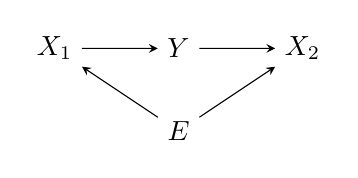
\begin{tikzpicture}[>=stealth, scale=1.05]
    \node (X1) at (-1.5,1) {$X_1$};
    \node (Y) at (0,1) {$Y$};
    \node (X2) at (1.5,1) {$X_2$};
    \node (E) at (0,0) {$E$};

    \draw[->] (X1) -- (Y);
    \draw[->] (Y) -- (X2);
    \draw[->] (E) -- (X1);
    \draw[->] (E) -- (X2);
\end{tikzpicture}
\end{minipage}\\[6pt]
where $\varepsilon_1, \varepsilon_Y, \varepsilon_2 \sim \mathrm{Unif}([0,1])$, mutually independent, and $\oplus$ denotes addition modulo $2$. Set $\Envtr = \{1, 2, 3\}$ and $\Env = \Envtr \cup \{8\}$.

Subset method: only $S = \{1\}$ is invariant, with $\P_e(Y = 1 \given X_1 = 1) = 3/4$ and $\P_e(Y = 1 \given X_1 = 0) = 1/4$ for all $e \in \Env$. The classifier $f_{\{1\}}$ achieves $3/4$ accuracy in every environment.

IRM: consider the representation $\Phi(x) \coloneq x_2$. Although $\P_e(Y = 1 \given X_2 = 1)$ varies across $\Envtr$, it stays above $1/2$ in every training environment, so the classifier $w = \mathrm{id}$ is Bayes-optimal under the $0$--$1$ loss in all $e \in \Envtr$.
% and $\Phi$ satisfies the IRM invariance criterion
The resulting accuracy ranges from $9/10$ to $7/10$ across $\Envtr$, exceeding the $3/4$ of $f_{\{1\}}$ on average. In the test environment $e = 8$, the accuracy of $w \circ \Phi$ drops to $1/5$.
%A subset method detects the non-invariance of $\{2\}$ from training data, while IRM uses the spurious representation because its invariance criterion does not capture the variation.
\end{example}


% In Ex.~\ref{ex:irm-vs-subset}, IRM accepts $\Phi$ as invariant because the Bayes-optimal classifier under $0$--$1$ loss does not change across $\Envtr$, although $Y \notindep E \given \Phi(X)$. The example shows that function-based invariance criteria can be weaker than the conditional invariance $Y \indep E \given X_S$ of Def.~\ref{def:inv_subset}, in the sense that they may accept representations $\Phi$ with $Y \notindep E \given \Phi(X)$; as a consequence, the function-view predictor $w \circ \Phi$ is outperformed by the subset-view predictor $f_{\{1\}}$ in worst-case accuracy on $\Env$. This specific failure can be avoided by replacing the $0$--$1$ loss with a loss strictly consistent for the mean functional, under which $\E_e[Y \given \Phi(X)]$ varies across $\Envtr$ and IRM rejects $\Phi$.

% (2) The subset view and the function view also allow for different types of extrapolation. For instance, when $E$ has more than one child, the function view typically extrapolates across values of $E$, while a subset method extrapolates also to environments in which the children of $E$ are intervened on separately. The following example illustrates this: the function view exploits a pattern on $\Envtr$ that does not persist on $\Env$.


% \linus{[rewrote the paragraph with your suggestions below]}
% \rml{In Ex.~\ref{ex:irm-vs-subset}, IRM accepts $\Phi$ as invariant because the Bayes-optimal classifier under $0$--$1$ loss does not change across $\Envtr$, although $Y \notindep E \given \Phi(X)$.
% \jonas{Here, it is outperformed by subset-based methods in terms of... However, one could 
% tackle (1) [DISCUSS?] by
% deviating from the proposal of IRM and ...}
% Under a loss strictly consistent for the mean functional, IRM would reject $\Phi$. \jonas{what  would then happen?}
% \jonas{[try to be even more clear about the conclusions drawn from the example]}
% The example nevertheless makes the point that function-based invariance criteria can be weaker 
% \jonas{[in which sense? maybe move a bit further up (as suggested?)]}
% than the conditional invariance used in the subset view.}

In Ex.~\ref{ex:irm-vs-subset}, IRM accepts $\Phi$ as invariant because the Bayes-optimal classifier under the $0$--$1$ loss does not change across $\Envtr$, although $Y \notindep E \given \Phi(X)$. This illustrates that function-based invariance criteria can be weaker than the invariance $Y \indep E \given X_S$ of Def.~\ref{def:inv_subset}. Here, $w \circ \Phi$ is outperformed by the subset-based $f_{\{1\}}$ in worst-case accuracy on $\Env$. However, one could tackle this by 
modifying the original IRM as follows: we could replace
%replacing 
the $0$--$1$ loss with a loss strictly consistent for the mean functional in IRM: under such a loss, IRM would reject $\Phi$ since $\E_e[Y \given \Phi(X)]$ varies across $\Envtr$. In this case, the representation $X \mapsto X_1$ would still satisfy the IRM criterion.




% \jonas{(2)
% The subset view and the function view allow for different types of extrapolations. For example, if there is a single $E$ with two children, a function view usually extrapolates in values of $E$. A subset method often comes with extrapolation guarantees even if the two children of $E$ are intervened on separately. We make formalize this statement with an example
% } 
% \rmj{Next, we provide an example where a function satisfies significantly stronger invariances \jonas{than what?}, however, its worst-case risk exceeds that of $f_{\SB(Y)}$. 
% We illustrate that the flexibility of the function view can have a downside: 
% a function has more potential 
% to exploit}
% \jonas{In that example, the function view exploits }
% a pattern on $\Envtr$ that does not persist on $\Env$. \linus{[I'm not sure whether "extrapolate" is the right word here if $E$ just indexed environments and we don't necessarily have something like $E \in \mathbb{R}$. With "a single $E$" did you mean that the environment acts in the same way on both children? Because in our setup we always assume a single $E$. What would you think about smt like this? ]
% \jonas{[can you try to make this even more precise? ``as'' seems to mean ``in the same way'' -- but what does this mean exactly? Indeed, what does it mean in the categorical E case?}
(2) The subset view and the function view differ in the class of test interventions they are robust to. For example, if $E$ has two children, the function view typically requires that the joint distribution of these children shifts with $E$ on $\Env$ 
as 
it does on $\Envtr$;
a subset method, by contrast, often comes with guarantees even when the two children of $E$ are intervened on separately; we make this precise with the following example, where the function view exploits a pattern on $\Envtr$ that does not persist on $\Env$.
\begin{example}[Worst-case suboptimality of an invariant $f$] \label{ex:strict-inequality}
Let $\mathcal{Y} = \mathbb{R}$, $\ell(y,q) = (y-q)^2$, and consider the following SCM over $(X_1, X_2, Y, E)$ whose structural assignments on $\Envtr$ are\\[0pt]
\begin{minipage}{0.49\textwidth}
\begin{align*}
    Y &\coloneq \varepsilon_Y, \\
    X_1 &\coloneq \delta_E + Y + \varepsilon_1, \\
    X_2 &\coloneq \delta_E + \varepsilon_2, \\
    \text{where }& \delta_E \in \mathbb{R} \text{ and } \varepsilon_Y, \varepsilon_1, \varepsilon_2 \stackrel{\text{i.i.d.}}{\sim} \mathcal{N}(0,1).
\end{align*}
\end{minipage}
\begin{minipage}{0.49\textwidth}
\centering
\vspace*{1.5em}
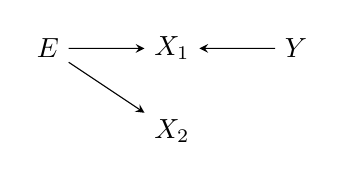
\begin{tikzpicture}[>=stealth, scale=1.05]
    \node (E) at (-1.5,1) {$E$};
    \node (X1) at (0,1) {$X_1$};
    \node (Y) at (1.5,1) {$Y$};
    \node (X2) at (0,0) {$X_2$};

    \draw[->] (E) -- (X1);
    \draw[->] (E) -- (X2);
    \draw[->] (Y) -- (X1);
\end{tikzpicture}
\end{minipage}\\[6pt]
Here, $\SB(Y) = \varnothing$, so $f_{\SB(Y)} = \E[Y] = 0$. The representation $\Phi(X) \coloneq X_1-X_2 = Y + \varepsilon_1 - \varepsilon_2$ is independent of $E$ on $\Envtr$, and the predictor $f(x) \coloneq \E[Y \given \Phi = x_1-x_2] = (x_1-x_2)/3$ is optimal for the squared loss on top of $\Phi$. For all $e \in \Envtr$, $R_e(f) = \frac{2}{3}< 1 = R_e(f_{\SB(Y)})$.
% \begin{equation} \label{eq:risk_inv}
%     R_e(f) = \E_e[(Y - f(X))^2]= \Var(Y \given \Phi) = 1 - \frac{\Cov(Y, \Phi)^2}{\Var(\Phi)} = \frac{2}{3}< 1 = R_e(f_{\SB(Y)}).
% \end{equation}



On $\Envtr$, $f$ satisfies several invariance properties: (i) $Y \indep E \given f(X)$, and thus $\E_e[Y \given \Phi(X)]$ does not depend on $e \in \Envtr$, so $\Phi$ satisfies the IRM invariance criterion of \citet[Def.~3]{arjovskyInvariantRiskMinimization2020}; (ii) $E \indep f(X)$; (iii) invariant residuals $Y - f(X) \indep E$, the invariance notion used by \citet{saengkyongamExploitingIndependentInstruments2022}; and (iv) invariance of the risks.

We now extend the SCM to $\Env$: for all $e\in\Envtr$, let $\Env$ contain an environment $e'$ in which the structural assignment of $X_1$ is replaced by $X_1\coloneq\tilde\varepsilon_1\sim\mathcal{N}(0,1)$, independent of $(Y,\varepsilon_1,\varepsilon_2)$, while the assignment of $X_2$ is unchanged. Then Asm.~\ref{as:A2} holds. In environment $e'$, $f(X)=(\tilde\varepsilon_1-\delta_{e'}-\varepsilon_2)/3$ is independent of $Y$. Furthermore, 
$R_{e'}(f) = 1 + (2 + \delta_{e'}^2)/9 > 1 = R_{e'}(f_{\SB(Y)}), $
and hence, $\sup_{e \in \Env}R_e(f) > \sup_{e\in\Env} R_e(f_{\SB(Y)})$, that is, Inequality~\eqref{eq:worst_case_statement} is strict. 
\end{example}

In Ex.~\ref{ex:strict-inequality}, $f$ exploits a pattern on $\Envtr$ that does not extend to $\Env$. Our setup in \Cref{sec:problem_setup} makes few structural assumptions on the interventions, and in this regime the subset view is robust under the intervention class considered here. \Cref{thm:worst_case} formalizes this. If the interventions are restricted to a known class, the function view can instead be preferable: anchor regression \citep{rothenhauslerAnchorRegressionHeterogeneous2020}, for instance, is worst-case optimal over a specific class of bounded shift interventions. But in this paper, we focus on the more general case.

(3)
The subset view is arguably more interpretable and transparent: it combines feature selection with standard supervised learning, rather than an opaque function of all covariates. In regulated settings such as credit scoring or clinical decision support, this simplifies auditing and certifying that prohibited features are not used, and makes individual predictions easier to explain. Only the variables in the chosen invariant subset $S \subseteq \{1, \ldots, d\}$ need to be measured at deployment.
% \rml{The choice of inputs also influences 
% \jonas{[do not understand this sentence]}
% the behavior of agents interacting with the model, as in the example of \Cref{sec:intro}: using causal features such as income encourages applicants to improve their actual creditworthiness, whereas using manipulable downstream variables invites gaming.}
Finally, the subset view can make the follower's potential actions
% \rmj{incentives}
more transparent, as the choice of which subset of covariates is used to construct $f$ influences the followers' behavior: as in \Cref{sec:intro}, using only causal features (such as safety equipment) means a follower can change their prediction only by genuinely changing $Y$, whereas including manipulable non-causal features (such as car color) lets them change the prediction without changing $Y$.
% \jonas{[owise +1]}








\subsection{Generalization to Ex.~\ref{ex:star_counterexample}} \label{sec:generalized_example}
The following proposition generalizes
Ex.~\ref{ex:star_counterexample}.
\begin{proposition} \label{prop:star_necessary}
Assume $\mathcal{Y} = \mathbb{R}$. Let $\G$ be a DAG over $(X_1, \ldots, X_d, Y, E)$ with $E$ a source node and no edge $E \to Y$, and let $\bar{\G}$ be the induced subgraph of $\G$ on $(X_1, \ldots, X_d, Y)$. If \eqref{eq:star} fails, then there exists an SCM with graph $\G$ and induced distribution $\P$, and a set of environments $\Env$
% \rml{a set of environments $\Env$ \jonas{[turn around SCM, $\G$ and $\Env$?]} and an SCM with graph $\G$ and induced distribution $\P$}
such that
(i) there exists $e_0 \in \Env$ under which $\P_{e_0}$ is faithful w.r.t.\ $\bar{\G}$,
(ii) the second part of Asm.~\ref{as:A2} holds (that is, for all $e \in \Env$ there exists an environment $e' \in \Env$ for which every $j \in \CH_\mathrm{int}(Y)$ is set independently of all other variables, with all other structural assignments unchanged), and
(iii) there exists a measurable $f \colon \mathcal{X} \to \mathbb{R}$ with $R_e(f) < R_e(f_{\SB(Y)})$ for all $e \in \Env$.
\end{proposition}

A proof can be found in \Cref{app:proof_prop:star_necessary}.


\subsection[Generalizing the result by Rojas-Carulla et al. (2018)]{Generalizing the result by \citet{rojas-carullaInvariantModelsCausal2018}}
\label{app:rojas}

The following proposition generalizes Thm.~4 by \citet{rojas-carullaInvariantModelsCausal2018}.


\begin{proposition}[Adversarial optimality] \label{prop:adversarial}
Let $S$ be an invariant subset of covariates, and let
$N \coloneq \{1, \ldots, d\} \setminus S$. Let $\mu$ be a dominating measure
on $\mathcal{X}$ such that $\mu = \mu_S \otimes \mu_N$ for some
measures $\mu_S$ on $\mathcal{X}_S$ and $\mu_N$ on $\mathcal{X}_N$
(such as Lebesgue or counting measures). Define $\mathcal{Q}_S$ to be
the family of all joint distributions $\Q$ of $(X,Y)$ on
$\mathcal{X} \times \mathcal{Y}$ such that
\begin{enumerate}[label=(\roman*)]
  \item $\E_\Q[Y \given X_S] = f_S(X_S)$ \quad $\Q$-almost surely,
  \item the marginal distribution of $X$ under $\Q$ is absolutely
        continuous with respect to $\mu$.
\end{enumerate}
Then the predictor $f_S$ satisfies
$$
  f_S \in
  \argmin_{\substack{f:\,\mathcal{X}\to\mathcal{A}\\
                      \mathrm{measurable}}}\;
  \sup_{\Q \in \mathcal{Q}_S}\,
  \E_{(X,Y)\sim\Q}\!\big[\ell(Y, f(X))\big].
$$
\end{proposition}
A proof can be found in \Cref{app:adversarial}.

% \subsection{Continuous variant of Ex.~\ref{ex:star_counterexample}} \label{app:cont_example}
% \linus{[bad title]}
% \linus{[work in progress]}

% \begin{proposition}
% Let $Y\in\{0,1\}$ with
% \[
% \mathbb P(Y=1)=\mathbb P(Y=0)=\tfrac12.
% \]
% Let
% \[
% g(x)=
% \begin{cases}
% -\beta d, & x<-d,\\
% \beta x, & -d\le x\le 1+d,\\
% \beta(1+d), & x>1+d.
% \end{cases}
% \]
% In the training environment, let
% \[
% X_2 = Y+\varepsilon_2,\qquad \varepsilon_2\sim \mathrm{Unif}[-d,d],
% \]
% and
% \[
% X_1 = Y + g(X_2) + \varepsilon_1,\qquad \varepsilon_1\sim \mathrm{Unif}[-c,c],
% \]
% where $\varepsilon_1,\varepsilon_2$ are independent of each other and of $Y$, and $0<\beta<1$.

% Assume
% \[
% c=\beta d,\qquad d=\frac{1+\beta}{4\beta}+\delta
% \]
% for some $\delta>0$, and define the train regression function
% \[
% m(x):=\mathbb E_{\mathrm{tr}}[Y\given X_1=x].
% \]

% In a test environment, let $X_2$ have an arbitrary distribution, possibly depending on $Y$, but the distribution of $Y$ and the structural assignment of $X_1$ stay the same (i.e.\ we consider an intervention on $X_2$).

% If
% \[
% \delta<\frac{3(1-7\beta)}{20\beta},
% \]
% then
% \[
% \mathbb E_{\mathrm{te}}\bigl[(Y-m(X_1))^2\bigr]
% \le
% \frac{2\beta+\frac83\beta\delta}{1+\beta+4\beta\delta}
% <\frac14.
% \]
% Hence the train conditional expectation $m(X_1)$ has strictly smaller test Brier risk than the mean predictor $1/2$.
% \end{proposition}

% \begin{proof}
% Under the training distribution,
% \[
% X_2=Y+\varepsilon_2
% \]
% with $\varepsilon_2\sim \mathrm{Unif}[-d,d]$, so
% \[
% X_2\in[-d,1+d]
% \qquad \text{almost surely.}
% \]
% Hence on the training support of $X_2$ we have $g(X_2)=\beta X_2$, and therefore
% \[
% X_1=Y+g(X_2)+\varepsilon_1
% =
% Y+\beta X_2+\varepsilon_1
% =
% \beta(Y+\varepsilon_2)+Y+\varepsilon_1
% =
% (1+\beta)Y+\eta,
% \]
% where
% \[
% \eta:=\beta\varepsilon_2+\varepsilon_1.
% \]

% Since $\varepsilon_2\sim \mathrm{Unif}[-d,d]$ and $c=\beta d$, both $\beta\varepsilon_2$ and $\varepsilon_1$ are uniform on $[-\beta d,\beta d]$. Therefore $\eta$ has triangular density
% \[
% f_\eta(t)=\frac{2\beta d-|t|}{4\beta^2d^2}\mathbf 1\{|t|\le 2\beta d\}.
% \]

% Let
% \[
% a:=1+\beta,\qquad s:=2\beta d.
% \]
% Then
% \[
% f_\eta(t)=\frac{s-|t|}{s^2}\mathbf 1\{|t|\le s\},
% \]
% and Bayes' rule gives
% \[
% m(x)=\mathbb E_{\mathrm{tr}}[Y\given X_1=x]
% =
% \frac{(s-|x-a|)_+}{(s-|x-a|)_+ + (s-|x|)_+},
% \]
% where $(u)_+:=\max\{u,0\}$.

% Because
% \[
% d=\frac{1+\beta}{4\beta}+\delta,
% \]
% we have
% \[
% s=2\beta d=\frac{1+\beta}{2}+2\beta\delta,
% \qquad
% w:=2s-a=4\beta\delta.
% \]
% Under the stated condition on $\delta$, we in particular have $0<\beta<1/7$, and hence
% \[
% \delta<\frac{1-\beta}{4\beta}.
% \]
% Therefore $s<a$. In this case,
% \[
% m(x)=
% \begin{cases}
% 0, & x\le a-s,\\[4pt]
% \dfrac{x-(a-s)}{w}, & a-s<x<s,\\[8pt]
% 1, & x\ge s.
% \end{cases}
% \]

% Now consider the test environment. Since $g$ is clamped outside $[-d,1+d]$,
% \[
% g(X_2)\in[-\beta d,\beta(1+d)]=[-c,\beta+c]
% \]
% almost surely, regardless of the test law of $X_2$.

% Fix $Y=0$, and write $U:=g(X_2)$. Conditional on $U=u$, we have
% \[
% X_1=u+\varepsilon_1,
% \qquad
% \varepsilon_1\sim \mathrm{Unif}[-c,c],
% \]
% so $X_1\given (U=u,Y=0)$ is uniform on $[u-c,u+c]$, an interval of length $2c=s$.

% Since $m$ is increasing, $m^2$ is also increasing, and therefore
% \[
% \mathbb E\bigl[m(X_1)^2\given U=u,Y=0\bigr]
% =
% \frac1s\int_{u-c}^{u+c} m(x)^2\,dx
% \]
% is maximized at the largest possible $u$, namely $u=\beta+c$. Hence
% \[
% \mathbb E\bigl[m(X_1)^2\given Y=0\bigr]
% \le
% \frac1s\int_{\beta}^{\beta+s} m(x)^2\,dx.
% \]

% We now decompose the interval $[\beta,\beta+s]$. Since
% \[
% a-s=\frac{1+\beta}{2}-2\beta\delta,
% \]
% the stated restriction on $\delta$ implies in particular
% \[
% \beta\le a-s.
% \]
% Thus $[\beta,\beta+s]$ consists of:
% \begin{itemize}
%     \item a region where $m(x)=0$,
%     \item the ramp interval $[a-s,s]$ of width $w=4\beta\delta$,
%     \item a region $[s,\beta+s]$ of length $\beta$ where $m(x)=1$.
% \end{itemize}
% Therefore
% \[
% \int_{\beta}^{\beta+s} m(x)^2\,dx
% =
% \int_{a-s}^{s}
% \left(\frac{x-(a-s)}{w}\right)^2\,dx
% +
% \int_s^{\beta+s}1\,dx.
% \]
% The first integral equals $w/3$, and the second equals $\beta$. Hence
% \[
% \mathbb E\bigl[m(X_1)^2\given Y=0\bigr]
% \le
% \frac{\beta+w/3}{s}
% =
% \frac{\beta+\frac43\beta\delta}{\frac{1+\beta}{2}+2\beta\delta}
% =
% \frac{2\beta+\frac83\beta\delta}{1+\beta+4\beta\delta}.
% \]

% By symmetry, the same bound holds for $Y=1$:
% \[
% \mathbb E\bigl[(1-m(X_1))^2\given Y=1\bigr]
% \le
% \frac{2\beta+\frac83\beta\delta}{1+\beta+4\beta\delta}.
% \]
% Therefore
% \[
% \mathbb E_{\mathrm{te}}\bigl[(Y-m(X_1))^2\bigr]
% \le
% \frac12\mathbb E\bigl[m(X_1)^2\given Y=0\bigr]
% +
% \frac12\mathbb E\bigl[(1-m(X_1))^2\given Y=1\bigr]
% \le
% \frac{2\beta+\frac83\beta\delta}{1+\beta+4\beta\delta}.
% \]

% It remains to compare with the mean predictor $1/2$, whose Brier risk is
% \[
% \mathbb E\bigl[(Y-\tfrac12)^2\bigr]=\tfrac14.
% \]
% Thus it suffices to require
% \[
% \frac{2\beta+\frac83\beta\delta}{1+\beta+4\beta\delta}<\frac14.
% \]
% This is equivalent to
% \[
% 8\beta+\frac{32}{3}\beta\delta<1+\beta+4\beta\delta,
% \]
% that is,
% \[
% 7\beta+\frac{20}{3}\beta\delta<1,
% \]
% or
% \[
% \delta<\frac{3(1-7\beta)}{20\beta},
% \]
% which is exactly the assumed condition. This proves the claim.
% \end{proof}



\appsection{Stabilized regression and classification}

\subsection{Invariance tests for classification} \label{app:invariance_tests}


We now provide detailed descriptions of the invariance tests that can be used for the methods described in \Cref{sec:learning_subset_predictors}. All tests target the conditional independence $H_{0,S}\colon Y \indep E \given X_S$ and return a $p$-value used as the invariance score $s_\mathrm{inv}(S)$. Each test can be used with different base models (such as logistic regression, random forests, or gradient boosting).


\subsubsection{Residual-based tests}

Residual-based tests fit a model $\hat{f}$ for $\E[Y \given X_S]$ on data pooled across environments, compute residuals $R = Y - \hat{f}(X_S)$, and test whether the distribution of $R$ depends on $E$.

\paragraph{Invariant Residual Distribution Test (IRD).}
Tests whether the mean of $R$ varies across environments using a one-way ANOVA $F$-test \citep[adapted from][]{heinze-demlInvariantCausalPrediction2018}.

\paragraph{\textsc{tram}-GCM.}
Applies the generalized covariance measure \citep{shahHardnessConditionalIndependence2018} to the residuals of both predicting $Y$ from $X_S$ and $E$ from $X_S$, testing whether their expected product is zero \citep{kookModelbasedCausalFeature2023}.

% \paragraph{Weighted GCM (WGCM).}
% Extends GCM by incorporating data-driven or fixed weight functions to improve power against nonlinear alternatives \citep{scheideggerWeightedGeneralisedCovariance2022}.

\subsubsection{Predictive-performance-based tests}

Predictive-performance-based tests check whether $E$ carries additional predictive information about $Y$ beyond $X_S$, or vice versa.

\paragraph{Invariant Target Prediction Test (ITP).}
Compares the ROC AUC of a classifier predicting $Y$ from $(X_S, E)$ against one using $X_S$ and permuted observations of $E$ via DeLong's test \citep{delongComparingAreasTwo1988} for correlated ROC curves \citep{heinze-demlInvariantCausalPrediction2018, salas-porrasIdentifyingCausesPyrocumulonimbus2022}. A significant AUC decrease upon permuting $E$ rejects invariance.

\paragraph{Invariant Environment Prediction Test (IEP).}
Reverses the direction and tests whether $Y$ helps predict $E$ given $X_S$. It compares the cross-entropy loss of a model predicting $E$ from $(X_S, Y)$ against one using $X_S$ and permuted observations of $Y$ via a paired $t$-test \citep[adapted from][]{heinze-demlInvariantCausalPrediction2018}.


\subsection{Algorithm} \label{app:SC_alg}

Stabilized regression \citep{pfisterStabilizingVariableSelection2021} uses a two-stage procedure to determine the weights $\hat{\omega}_S$ for $S \subseteq \{1, \ldots, d\}$. 
We now propose
stabilized classification, which is directly ported from stabilized regression and proceeds in the same way.

\paragraph{Stage 1: invariance.} First, we estimate the collection of invariant subsets by computing an invariance score $s_\mathrm{inv}(S)$ for each subset $S \subseteq \{1, \ldots, d\}$. Then, we define the empirically invariant subsets as $\hat{\mathcal{I}}_{\Envtr} \coloneq \big\{S \subseteq \{1, \ldots, d\} \given s_\mathrm{inv}(S) \geq \alpha_\mathrm{inv} \big\}$, where the cutoff $\alpha_\mathrm{inv} \in \mathbb{R}$ is a tuning parameter. \Cref{sec:learning_subset_predictors} discusses suitable scores $s_\mathrm{inv}(S)$ for this step. Because iterating over all $2^d$ subsets becomes computationally prohibitive even for moderate $d$, an optional variable screening step (e.g., using $\ell_1$-penalized logistic regression) can be applied to reduce the candidate covariate set before computing the invariance scores.


\paragraph{Stage 2: prediction performance.}
We estimate the subsets with best prediction performance among those in $\hat{\mathcal{I}}_{\Envtr}$. We evaluate the prediction performance of each $S \in \hat{\mathcal{I}}_{\Envtr}$ using a score $s_\mathrm{pred}(S)$, such as the negative binary cross-entropy loss on the training data. We then define the final set of selected subsets as $\hat{\mathcal{C}}_{\Envtr} \coloneq \big\{ S \in \hat{\mathcal{I}}_{\Envtr} \given s_\mathrm{pred}(S) \geq c(\alpha_\mathrm{pred}) \big\}$, where $c(\alpha_\mathrm{pred})$ is a cutoff threshold. Following \citet{pfisterStabilizingVariableSelection2021}, we determine $c(\alpha_\mathrm{pred})$ using a bootstrap procedure. Let $\hat{S}_\mathrm{max} \coloneq \argmax_{S \in \hat{\mathcal{I}}_{\Envtr}} s_\mathrm{pred}(S)$ denote the invariant subset with best prediction performance. We generate $B$ bootstrap samples from the training data, compute the prediction scores for $\hat{S}_\mathrm{max}$ on each sample, and set $c(\alpha_\mathrm{pred})$ to the $\alpha_\mathrm{pred}$-quantile of these bootstrap scores. Therefore, the hyperparameters $\alpha_\mathrm{inv}, \alpha_\mathrm{pred} \in (0,1)$ control the size of the ensemble. Finally, we use uniform weights $\hat{\omega}_S$ over the selected subsets in $\hat{\mathcal{C}}_{\Envtr}$: $\hat{\omega}_S \coloneq \frac{1}{|\hat{\mathcal{C}}_{\Envtr}|}$ for $S \in \hat{\mathcal{C}}_{\Envtr}$ and $\hat{\omega}_S \coloneq 0$ otherwise. Algorithm~\ref{alg:SC} summarizes the full procedure. 


\begin{algorithm}[t]
\caption{Stabilized classification (SC) \label{alg:SC}}
\begin{algorithmic}[1]
\Require data $\mathcal{D} = (x_i, y_i, e_i)_{i=1}^n$ from $\Envtr$; hyperparameters $\alpha_\mathrm{inv}, \alpha_\mathrm{pred} \in (0,1)$, $B \in \mathbb{N}$
\State (optional) perform variable screening to reduce $d$ \label{line:var_screening}
\For{all $S \subseteq \{1, \ldots, d\}$}
    \State compute invariance score $s_\mathrm{inv}(S)$ using $\mathcal{D}$
\EndFor
\State $\hat{\mathcal{I}}_{\Envtr} \gets \big\{S \subseteq \{1, \ldots, d\} \given s_\mathrm{inv}(S) \geq \alpha_\mathrm{inv} \big\}$ \Comment{invariance}
\For{all $S \in \hat{\mathcal{I}}_{\Envtr}$}
    \State fit base classifier $\hat{f}_S$ on $\mathcal{D}$
    \State compute predictive score $s_\mathrm{pred}(S)$ on $\mathcal{D}$
\EndFor
\State $\hat{S}_\mathrm{max} \gets \argmax_{S \in \hat{\mathcal{I}}_{\Envtr}} s_\mathrm{pred}(S)$
\State compute cutoff $c(\alpha_\mathrm{pred})$ as the $\alpha_\mathrm{pred}$-quantile of $B$ bootstrap scores for $\hat{S}_\mathrm{max}$
\State $\hat{\mathcal{C}}_{\Envtr} \gets \big\{S \in \hat{\mathcal{I}}_{\Envtr} \given s_\mathrm{pred}(S) \geq c(\alpha_\mathrm{pred}) \big\}$ \Comment{prediction performance}
\State assign weights $\hat{\omega}_S \gets \frac{1}{|\hat{\mathcal{C}}_{\Envtr}|} \bm{1}\big\{S \in \hat{\mathcal{C}}_{\Envtr} \big\}$
\item[\textbf{Output:}] base estimators $\hat{f}_S$ and weights $\hat{\omega}_S$ defining the ensemble $\hat{f}^{\mathrm{SC}}$
\end{algorithmic}
\end{algorithm}










\appsection{Proofs}\label{app:proofs}

The following lemma serves as a generalization of the orthogonality of the conditional expectation (used for regression ($Y \in \mathbb{R}$) with the MSE) to regression and binary classification with loss functions strictly consistent for the mean functional. It is used for several results.

\begin{lemma}
\label{lem:bayes_restricted}
Let $Y$ and $W$ be random variables on a probability space
$(\Omega, \mathcal{F}, \P)$, with $Y$ taking values in $\mathcal{Y}$
and integrable.
Let $Z$ be a $\sigma(W)$-measurable random variable
taking values in $\mathcal{A}$. If $\ell$ is strictly consistent for the mean
functional, then
\begin{equation*}
  \mathbb{E}\bigl[\ell(Y,Z)\bigr]
  \;\geq\;
  \mathbb{E}\bigl[\ell\bigl(Y,\mathbb{E}[Y\given W]\bigr)\bigr],
\end{equation*}
where $\E[\cdot]$ denotes expectation under $\P$.
If both expectations are finite, equality holds if and only if
$Z=\mathbb{E}[Y\given W]$ almost surely.
\end{lemma}

\begin{proof}[Proof of Lem.~\ref{lem:bayes_restricted}]
For all $q \in \mathcal{A}$ and probability distributions $F$ on $\mathcal{Y}$ with finite mean $\E_{Y \sim F}[Y]$, define
$$
L(F, q) \coloneq \E_{Y \sim F}[\ell(Y, q)].
$$
Let $F_W$ denote the conditional distribution of $Y$ given $W$ \citep[Thm.~8.5]{kallenbergFoundationsModernProbability2021}. Its mean equals $\E[Y \given W]$ almost surely. Conditional on $W$, the random variable $Z$ acts as a constant since $Z$ is $\sigma(W)$-measurable, so almost surely, 
$$
\E[\ell(Y, Z) \given W] = L(F_W, Z).
$$

By strict consistency of $\ell$, for every distribution $F$ with finite mean,
$q \mapsto L(F, q)$ is uniquely minimized at $q = \E_{Y \sim F}[Y]$.
Since this holds for every $F$, it holds pointwise for the random
conditional distribution $F_W$ for almost every $\omega \in \Omega$.
Thus, almost surely, 
$$
  L(F_W, Z) \geq L(F_W, \E[Y \given W])
  =
  \E\big[\ell(Y, \E[Y \given W]) \given W\big],
$$
with equality if and only if $Z = \E[Y \given W]$ almost surely. Taking
expectations, $\E[\ell(Y,Z)] \geq \E[\ell(Y,\E[Y \given W])]$. For the equality
case, assume both expectations are finite and equal. Then the
nonnegative random variable
$D := \E[\ell(Y,Z)\given W] - \E[\ell(Y,\E[Y \given W])\given W]$ satisfies
$\E[D] = 0$, hence $D = 0$ almost surely, and pointwise strictness
gives $Z = \E[Y \given W]$ almost surely. The converse is immediate.
\end{proof}

\subsection{Proof of Lem.~\ref{lem:stable_region_opt}}
We first state and prove a lemma. The d-separation statement
for $\SB(Y)$ is also shown in the proof of
\citet[Thm.~3.5]{pfisterStabilizingVariableSelection2021}; we include
the argument for completeness and extend it to $\DEYforb^C$.

\begin{lemma}\label{lemma:d-sep}
The subsets $\DEYforb^C$ and $\SB(Y)$ satisfy the d-separations
$$
  Y \dsep{\G} E \given \DEYforb^C
  \qquad\text{and}\qquad
  Y \dsep{\G} E \given \SB(Y).
$$
\end{lemma}
\begin{remark} \label{rem:SB_in_different_DAGs}
    The statement and proof of Lem.~\ref{lemma:d-sep} only use that $E$ is a source node in $\G$ with no edge $E \to Y$, and apply unchanged to any DAG over $(X_1, \ldots, X_d, Y, E)$ with these properties, provided $\DEYforb$ and $\SB(Y)$ are computed in that DAG.
\end{remark}

\begin{proof}[Proof of Lem.~\ref{lemma:d-sep}]
We prove both statements simultaneously. Let
$S \in \{\DEYforb^C,\, \SB(Y)\}$ and recall that
$\PA(Y) \subseteq S \subseteq \DEYforb^C$ from \eqref{eq:stable_blanket_decomp}. Consider an arbitrary path from $E$
to $Y$ in $\G$. Since $E$ is a source node and not a parent of $Y$,
the path contains an intermediate node $i$ adjacent to $Y$. We
distinguish two cases.

\paragraph{Case 1. $E \rightarrow ~\cdots~ i \rightarrow Y$.}
Then $i \in \PA(Y) \subseteq S$, so the path is blocked.

\paragraph{Case 2. $E \rightarrow ~\cdots~ i \leftarrow Y$.}
Since $E$ is a source node, the path contains at least one collider.
\begin{itemize}
  \item If $i \in \DEYforb$: let $k$ be the collider closest to
    $Y$ on the path (possibly $k = i$). The segment from $Y$ to $k$ is
    directed $(Y \rightarrow i \rightarrow \cdots \rightarrow k)$, so $k \in \DE(i) \cup \{i\}$. Since
    $i \in \DEYforb$, and because descendants of nodes in
    $\DEYforb$ are again in $\DEYforb$, we have
    $\DE(k) \cap \DEYforb^C = \varnothing$. Hence neither $k$ nor any
    descendant of $k$ lies in $S \subseteq \DEYforb^C$, and the path
    is blocked.
  \item If $i \in \DEYforb^C$: then
    $i \in \CH(Y) \cap \DEYforb^C \subseteq S$. If $i$ is not a
    collider, the path is blocked because $i \in S$. If $i$ is a
    collider, the path has the form
    $E \to \cdots j \to i \leftarrow Y$ for some $j$ with $i \neq j \neq E$ (if
    $j = E$, then $i \in \CH(E) \cap \CH(Y) = \CH_\mathrm{int}(Y)$,
    contradicting $i \in \DEYforb^C$). Then
    $j \in \PA(\CH(Y) \cap \DEYforb^C) \subseteq \SB(Y)$ by
    \eqref{eq:stable_blanket_decomp}, and $j \in \DEYforb^C$ since
    $\DEYforb$ is closed under descendants. Thus $j \in S$, and since
    $j$ is a non-collider on the path, the path is blocked.
\end{itemize}
\end{proof}


\begin{proof}[Proof of Lem.~\ref{lem:stable_region_opt}]
By Lem.~\ref{lemma:d-sep} and the global Markov property,
$\DEYforb^C$ and $\SB(Y)$ are invariant subsets. In particular, for
all $e \in \Env$, $\E_e[Y \given X_{\DEYforb^C}]$ and
$\E_e[Y \given X_{\SB(Y)}]$ do not depend on~$e$. By definition of
$\SB(Y)$ \citep[Def.~3.4]{pfisterStabilizingVariableSelection2021}, for all $j \in \DEYforb^C \setminus \SB(Y)$ the
d-separation $j \dsep{\G} Y \given \SB(Y)$ holds. Thus,
$ \big(\DEYforb^C \setminus \SB(Y)\big) \dsep{\G} Y \given \SB(Y)$, so by the global Markov property,
$$
  X_{\DEYforb^C \setminus \SB(Y)} \indep Y \given X_{\SB(Y)}
$$
holds under $\P_e$ for all $e \in \Env$.
Doob's conditional independence property
\citep[Thm.~8.9]{kallenbergFoundationsModernProbability2021} then
yields that almost surely,
\begin{equation} \label{eq:Doob}
  \E[Y \given X_{\DEYforb^C}]
   = 
  \E[Y \given X_{\SB(Y)}, X_{\DEYforb^C \setminus \SB(Y)}]
   = 
  \E[Y \given X_{\SB(Y)}]
   = 
  f_{\SB(Y)}(X).
\end{equation}

Let $e \in \Env$ and let $f\colon \mathcal{X} \to \mathcal{A}$ be
$\sigma(X_{\DEYforb^C})$-measurable. Applying
Lem.~\ref{lem:bayes_restricted} under $\P_e$ with $W = X_{\DEYforb^C}$
and $Z = f(X)$ gives
$$
  R_e(f)
   \geq 
  \E_e \bigl[\ell(Y,  \E[Y \given X_{\DEYforb^C}])\bigr]
   \stackrel{\eqref{eq:Doob}}{=} 
  R_e(f_{\SB(Y)}).
$$
Since $e$ and $f$ were arbitrary, we obtain the result.
\end{proof}


\subsection{Proof of \texorpdfstring{\Cref{thm:PA_vs_SB_game}}{Theorem~\ref{thm:PA_vs_SB_game}}}
\begin{proof}[Proof of \Cref{thm:PA_vs_SB_game}]
For (i), $\Env^*(f) = \argmax_{e \in \Env} R_e(f)$, so $\sup_{e \in \Env^*(f)} R_e(f) = \sup_{e \in \Env} R_e(f)$ for every $f$. By Lem.~\ref{lem:stable_region_opt}, $R_e(f_{\SB(Y)}) \leq R_e(f_{\PA(Y)})$ for all $e \in \Env$, and taking suprema gives the claim.

For (ii), since $\PA(Y)$ and $\SB(Y)$ are invariant, the tower property gives $\E_e[f_{\PA(Y)}(X)] = \E_e[f_{\SB(Y)}(X)] = \E_e[Y]$ for all $e \in \Env$. Hence $\Vfoll_e(f_{\PA(Y)}) = \Vfoll_e(f_{\SB(Y)})$ for all $e$, which implies $\Env^*(f_{\PA(Y)}) = \Env^*(f_{\SB(Y)})$. Therefore
\[
    \sup_{e \in \Env^*(f_{\SB(Y)})} R_e(f_{\SB(Y)})  \leq  \sup_{e \in \Env^*(f_{\PA(Y)})} R_e(f_{\PA(Y)}),
\]
where the inequality uses Lem.~\ref{lem:stable_region_opt}.
\end{proof}


\subsection{Proof of Lem.~\ref{lem:augmentation}} \label{app:proof_augmentation}
\begin{proof}[Proof of Lem.~\ref{lem:augmentation}]
Since $A_j \subseteq \DEforbg{\G_0}^C \setminus \{Y, E\}$ for all $j$, we have $\CH_{\G}(Y) = \CH_{\G_0}(Y)$, $\CH_{\G}(E) = \CH_{\G_0}(E)$, and $\CH_\mathrm{int}(Y)$ is the same in $\G$ and $\G_0$.

First, we show $\DEforbg{\G} = \DEforbg{\G_0}$. The inclusion $\DEforbg{\G_0} \subseteq \DEforbg{\G}$ holds because adding edges can only enlarge the set of descendants. For the reverse, assume by contradiction that there exists $i \in \DEforbg{\G}$ with $i \notin \DEforbg{\G_0}$. Then, there exists a directed path in $\G$ from some $j \in \CH_\mathrm{int}(Y)$ to $i$ that uses at least one edge only existing in $\G$ (since this path does not exist in $\G_0$). Let $k \to l$ be the first such edge on the path (with $k \in A_l \subseteq \DEforbg{\G_0}^C$). The segment $j \to \cdots \to k$ uses only edges of $\G_0$, so $k \in \DE_{\G_0}(\CH_\mathrm{int}(Y)) \cup \CH_\mathrm{int}(Y) = \DEforbg{\G_0}$. This contradicts $k \in A_l \subseteq \DEforbg{\G_0}^C$.

Second, we show $\SBg{\G} = \SBg{\G_0}$. By \eqref{eq:stable_blanket_decomp}, the stable blanket $\SBg{\G_0}$ is the union of $\PA_{\G_0}(Y)$, $\CH_{\G_0}(Y) \setminus \DEforbg{\G_0}$, and $\PA_{\G_0}(\CH_{\G_0}(Y) \setminus \DEforbg{\G_0})$. Regarding the first set, $\PA_{\G}(Y) = \PA_{\G_0}(Y)$ because no intervention on $Y$ takes place. The second is unchanged in $\G$ since $\DEforbg{\G} = \DEforbg{\G_0}$ and $\CH_{\G}(Y) = \CH_{\G_0}(Y)$. The third is unchanged in $\G$ since every new edge points into $\CH_{\G_0}(E)$, and $\CH_{\G_0}(E) \cap (\CH_{\G_0}(Y) \setminus \DEforbg{\G_0}) = \varnothing$ since $\CH_{\G_0}(E) \cap \CH_{\G_0}(Y) = \CH_\mathrm{int}(Y) \subseteq \DEforbg{\G_0}$. Hence, no new edge enters $\CH_{\G_0}(Y) \setminus \DEforbg{\G_0}$, and $\PA_{\G}(\CH_{\G}(Y) \setminus \DEforbg{\G}) = \PA_{\G_0}(\CH_{\G_0}(Y) \setminus \DEforbg{\G_0})$.

Finally, $Y \dsep{\G} E \given \SBg{\G_0}$ follows since $\SBg{\G} = \SBg{\G_0}$ and by Lem.~\ref{lemma:d-sep} and Rmk.~\ref{rem:SB_in_different_DAGs}, $Y \dsep{\G} E \given \SBg{\G}$.
\end{proof}

% \begin{proof}
% Suppose every new edge is of the form $k \to j$ for $j \in {\CH}_{\G}(E)$ and $k \in {\DE_{\G}(Y)}_{\mathrm{forb}}^C$, and $\G^+$ is acyclic.
% \begin{itemize}
%     \item ${\CH}_{\G}(Y) = {\CH}_{\G^+}(Y)$ holds because $X_k \neq Y$.
%     \item ${\CH}_{\mathrm{int}}(Y)$ is the same in $\G$ and $\G^+$ since $X_k \neq E$.
%     \item ${\DE_{\G}(Y)}_{\mathrm{forb}} = {\DE_{\G^+}(Y)}_{\mathrm{forb}}$:
%     \begin{itemize}
%         \item We have ${\DE_{\G}(Y)}_{\mathrm{forb}} = {\CH}_{\mathrm{int}}(Y) \cup {\DE}_{\G}({\CH}_{\mathrm{int}}(Y))$. By adding edges, we can only add descendants, so ${\DE_{\G}(Y)}_{\mathrm{forb}} \subseteq {\DE_{\G^+}(Y)}_{\mathrm{forb}}$.
%         \item Assume by contradiction that $ {\DE_{\G^+}(Y)}_{\mathrm{forb}} \not\subseteq {\DE_{\G}(Y)}_{\mathrm{forb}}$.
%         \item This implies $\exists i \in {\DE_{\G^+}(Y)}_{\mathrm{forb}}$ with $i \notin {\DE_{\G}(Y)}_{\mathrm{forb}}$.
%         \item This implies there exists a directed path in $\G^+$ from some $j \in {\CH}_{\mathrm{int}}(Y)$ to $i$ that does not exist in $\G$.
%         \item The path must use at least one newly added edge; let $k \to l$ be the first such edge (with $k \in {\DE_{\G}(Y)}_{\mathrm{forb}}^C$).
%         \item Thus, the directed path $j \to \dots \to k$ exists in $\G$.
%         \item This implies $k \in {\DE}_{\G}(j) \subseteq {\DE}_{\G}({\CH}_{\mathrm{int}}(Y)) \subseteq {\DE_{\G}(Y)}_{\mathrm{forb}}$.
%         \item This contradicts $k \in {\DE_{\G}(Y)}_{\mathrm{forb}}^C$.
%     \end{itemize}
%     \item ${\SB}_{\G}(Y) = {\SB}_{\G^+}(Y)$:
%     \begin{itemize}
%         \item ${\PA}_{\G}(Y) = {\PA}_{\G^+}(Y)$ holds because we don't intervene on $Y$.
%         \item We also know ${\CH}_{\G^+}(Y) \setminus {\DE_{\G^+}(Y)}_{\mathrm{forb}} = {\CH}_{\G}(Y) \setminus {\DE_{\G}(Y)}_{\mathrm{forb}}$ from before.
%         \item Since new edges point into ${\CH}_{\G}(E)$ and ${\CH}_{\G}(E) \cap ({\CH}_{\G}(Y) \setminus {\DE_{\G}(Y)}_{\mathrm{forb}}) = \varnothing$, we have that ${\PA}_{\G^+}({\CH}_{\G^+}(Y) \setminus {\DE_{\G^+}(Y)}_{\mathrm{forb}}) = {\PA}_{\G}({\CH}_{\G}(Y) \setminus {\DE_{\G}(Y)}_{\mathrm{forb}})$.
%         \item Consequently, ${\SB}_{\G}(Y) = {\SB}_{\G^+}(Y)$.
%     \end{itemize}
%     \item The fact that $Y \dsep{\G^+} E \given \SB_{\G}(Y)$ holds follows from $Y \dsep{\G^+} E \given \SB_{\G^+}(Y)$ (since $\SB_{\G^+}(Y)$ is the stable blanket in $\G^+$) and $\SB_{\G}(Y) = \SB_{\G^+}(Y)$.
% \end{itemize}
% \end{proof}





\subsection{Proof of Thm.~\ref{thm:worst_case}}


We first state and prove a lemma. 

\begin{lemma}[Asm.~\ref{as:A2} implies
Asm.~\ref{as:A1}]
\label{lem:A2_implies_A1}
If Asm.~\ref{as:A2} holds, then for every $e \in \Env$ the
environment $e'$ provided by Asm.~\ref{as:A2} satisfies both
conditions of Asm.~\ref{as:A1}.
\end{lemma}
\begin{proof}[Proof of Lem.~\ref{lem:A2_implies_A1}]
Fix an arbitrary $e \in \Env$ and let $e' \in \Env$ be the corresponding environment provided by
Asm.~\ref{as:A2}, in which for all
$j \in \CH_\mathrm{int}(Y)$, we set $X_j \coloneq \Tilde{\varepsilon}_j$ with $\Tilde{\varepsilon}_j$ independent of all other variables, removing incoming edges to $\CH_\mathrm{int}(Y)$ in $\G$. All other structural assignments are unchanged. Let $\G'$ denote the resulting graph. Unless stated otherwise, all graph-theoretic notation such as $\PA(\cdot)$ refers to the original graph $\G$. Quantities defined with respect to $\G'$ are marked explicitly.

We first verify that Asm.~\ref{as:A1}~(i) holds.
Since $\DEYforb$ is closed under descendants, no node in
$\SB(Y) \subseteq \DEYforb^C$ is a descendant of any node in
$\CH_\mathrm{int}(Y)$. Because only the structural assignments of
$\CH_\mathrm{int}(Y)$ are modified in $e'$, the marginal distribution of
$X_{\SB(Y)}$ is the same under $\P_e$ and $\P_{e'}$.

To verify Asm.~\ref{as:A1}~(ii), we need to verify $Y \indep X_{\DEYforb} \given X_{\DEYforb^C}$ under $\P_{e'}$. Since $\P_{e'}$ is generated by the
modified SCM, it is Markov with respect to $\G'$. It therefore suffices
to show that $Y \dsep{\G'} \DEYforb \given \DEYforb^C$. Consider an arbitrary path in $\G'$ from $Y$ to some $j \in \DEYforb$, and let
$i$ be the node adjacent to $Y$ on this path.
\begin{itemize}
    \item If $Y \leftarrow i$, then $i \in \PA(Y) \subseteq \DEYforb^C$, so the path is blocked by $\DEYforb^C$.
    \item If $Y \to i$ with $i \in \CH(Y) \setminus \DEYforb^C$, then
    $i \in \DEYforb$, and
    condition~\eqref{eq:star} gives
    $i \in \CH_\mathrm{int}(Y)$. But in $\G'$ the edge $Y \to i$ is
    deleted, so this path does not exist.
    \item If $Y \to i$ with $i \in \CH(Y) \cap \DEYforb^C$, then if $i$ is a
    non-collider, the path is blocked since $i \in \DEYforb^C$. If
    $i$ is a collider, the path has the form
    $Y \to i \leftarrow k \cdots $ for some
    $k \in \PA_{\G'}(i) \setminus \{Y\}$. Since $i \in \CH(Y) \cap \DEYforb^C$, the node $i$ is not intervened on, hence $\PA_{\G'}(i) = \PA(i)$. Therefore,  
    $k \in \PA(\CH(Y) \cap \DEYforb^C) \subseteq \SB(Y)
    \subseteq \DEYforb^C$
    by~\eqref{eq:stable_blanket_decomp}. Since $k$ is a non-collider
    on the path, the path is blocked.
\end{itemize}
Since every path is blocked,
$Y \dsep{\G'} \DEYforb \given \DEYforb^C$, and the global Markov
property gives
$Y \indep X_{\DEYforb} \given X_{\DEYforb^C}$ under $\P_{e'}$.
\end{proof}



\begin{proof}[Proof of \Cref{thm:worst_case}]
By Lem.~\ref{lem:A2_implies_A1}, Asm.~\ref{as:A2} implies
Asm.~\ref{as:A1}, so it suffices to prove the claim under
Asm.~\ref{as:A1}. Let $f\colon \mathcal{X} \to \mathcal{A}$ be
an arbitrary measurable predictor. Fix $e \in \Env$ and let
$e' \in \Env$ be the corresponding environment provided by Asm.~\ref{as:A1}.
Applying Lem.~\ref{lem:bayes_restricted} under $\P_{e'}$ with $W = X$
and $Z = f(X)$,
\begin{equation} \label{eq:proper_step}
  R_{e'}(f)
   \geq 
  \E_{e'} \bigl[\ell(Y,  \E_{e'}[Y \given X])\bigr].
\end{equation}
By Asm.~\ref{as:A1}~(ii),
$Y \indep X_{\DEYforb} \given X_{\DEYforb^C}$ under $\P_{e'}$, so by Doob's conditional independence property
\citep[Thm.~8.9]{kallenbergFoundationsModernProbability2021},
$\E_{e'}[Y \given X] = \E_{e'}[Y \given X_{\DEYforb^C}]$ almost surely. Since
$\DEYforb^C$ is invariant by Lem.~\ref{lemma:d-sep} and the global Markov property,
$\E_{e'}[Y \given X_{\DEYforb^C}] = \E[Y \given X_{\DEYforb^C}]$, and
\eqref{eq:Doob} from the proof of Lem.~\ref{lem:stable_region_opt} gives $\E[Y \given X_{\DEYforb^C}] = f_{\SB(Y)}(X)$ almost surely.
Substituting into \eqref{eq:proper_step} yields
$$
  R_{e'}(f)  \geq  R_{e'}(f_{\SB(Y)}).
$$
It remains to show $R_{e'}(f_{\SB(Y)}) = R_e(f_{\SB(Y)})$. Since the marginal distribution of $X_{\SB(Y)}$ and the conditional distribution of $Y \given X_{\SB(Y)}$ are the same under $\P_e$ and $\P_{e'}$ by Asm.~\ref{as:A1}~(i) and the invariance of $\SB(Y)$, the distribution of $(Y, X_{\SB(Y)})$ is the same under $\P_{e'}$ and $\P_e$. Since $\ell(Y, f_{\SB(Y)}(X))$ is a measurable function of
$(Y, X_{\SB(Y)})$, the risks are equal.

Consequently, $\sup_{e'' \in \Env} R_{e''}(f) \geq R_{e'}(f) \geq R_e(f_{\SB(Y)})$.
Since $e$ was arbitrary, taking the supremum over $e$ on the
right-hand side yields \eqref{eq:worst_case_statement}. 
\end{proof}



\subsection{Proof of Prop.~\ref{prop:asymptotic}}

\begin{proof}[Proof of Prop.~\ref{prop:asymptotic}]
Fix an arbitrary predictor $f \colon \mathcal{X} \to \mathcal{A}$, $e \in \Env$, and let $(e'_j)_{j \geq 1}$ be the associated sequence from the assumption.
For all $j$, by Lem.~\ref{lem:bayes_restricted} applied under $\P_{e'_j}$ with
$W = X$ and $Z = f(X)$,
$$ R_{e'_j}(f) \geq R_{e'_j}(\mu_{e'_j}). $$
Since $\SB(Y)$ is invariant, the conditional distribution of
$Y \given X_{\SB(Y)}$ is the same in every environment. Together
with Condition~(i), the joint distribution of $(Y, X_{\SB(Y)})$ is the
same under $\P_e$ and $\P_{e'_j}$. Because
$\ell(Y, f_{\SB(Y)}(X))$ is a measurable function of
$(Y, X_{\SB(Y)})$, it follows that for all $j$,
$$ R_{e'_j} \bigl(f_{\SB(Y)}\bigr) =
  R_e \bigl(f_{\SB(Y)}\bigr). $$
By Condition~(ii), for all $\varepsilon>0$ there exists $N$ such that for all $j \geq N$, $R_{e'_j}\bigl(f_{\SB(Y)}\bigr)-R_{e'_j}(\mu_{e'_j})< \varepsilon$. Consequently,
\[
  R_{e'_j}(f)
  \geq
  R_e\bigl(f_{\SB(Y)}\bigr)
  -
  \Bigl(
    R_{e'_j}\bigl(f_{\SB(Y)}\bigr)-R_{e'_j}(\mu_{e'_j})
  \Bigr)
  \geq R_e\bigl(f_{\SB(Y)}\bigr) - \varepsilon.
\]
Therefore, for all $\varepsilon>0$, we have $\sup_{e'' \in \Env} R_{e''}(f) \geq R_e\bigl(f_{\SB(Y)}\bigr) - \varepsilon$. Letting $\varepsilon \to 0$ and taking the supremum over $e \in \Env$ ($e$ was arbitrary) yields \eqref{eq:worst_case_statement}.
\end{proof}







% \subsection{Proof of Equation~\texorpdfstring{\eqref{eq:stable_blanket_decomp}}{(\ref*{eq:stable_blanket_decomp})}}
% \label{app:stable_blanket_expression}

% \begin{proof}
% We wish to show that $\SB(Y) = \tilde{S}$, where
% $$ \tilde{S} \coloneq \PA(Y) \cup \Big(\CH(Y) \cap \Nint \Big) \cup \PA\Big(\CH(Y) \cap \Nint \Big). $$Recall that $\SB(Y)$ is defined as the smallest subset $S \subseteq \Nint$ satisfying
% \begin{equation} \label{eq:d-sep_cond}
%     \text{for all }j \in \Nint \setminus S: ~~~ j \dsep{\G} Y \given S.
% \end{equation}
% We prove $\SB(Y) = \tilde{S}$ by first showing $\tilde{S} \subseteq \SB(Y)$ and then that $S = \tilde{S}$ satisfies \eqref{eq:d-sep_cond}. 
% \paragraph{Step 1. Show $\Tilde{S} \subseteq \SB(Y)$:}
% Since nodes $\PA(Y) \subseteq \Nint$ are adjacent to $Y$ in $\G$, we require $\PA(Y) \subseteq \SB$ for \eqref{eq:d-sep_cond} to hold for $S = \SB(Y)$. The same argument shows that $\CH(Y) \cap \Nint \subseteq \SB(Y)$. As noted above, $\PA(\CH(Y) \cap \Nint ) \subseteq \Nint$. Since $\CH(Y) \cap \Nint \subseteq \SB(Y)$, and these nodes are colliders on any path between $\PA(\CH(Y) \cap \Nint )$ and $Y$, we also require $\PA(\CH(Y) \cap \Nint ) \subseteq \SB(Y)$. Thus, $\tilde{S} \subseteq \SB(Y)$.
% \paragraph{Step 2. Verify \eqref{eq:d-sep_cond} for $S= \Tilde{S}$:}
% Consider any path between $Y$ and $j \in \Nint \setminus \tilde{S}$. We distinguish two cases.
% \begin{itemize}
%     \item Incoming edge ($j ~\cdots~ \rightarrow Y$): Since $j \notin \PA(Y)$, the path must pass through some $i \in \PA(Y) \subseteq \Tilde{S}$, which blocks it.
%     \item Outgoing edge ($j ~\cdots~ \leftarrow Y$): Observe that $j \in \Nint$ cannot be a child of $Y$ because $\CH(Y) \cap \Nint \subseteq \Tilde{S}$, and we assumed $j \in \Nint \setminus \Tilde{S}$. Therefore, there exists some $i \in \{1, \ldots, d\} \setminus\{j\}$ such that the path is of the form $ j ~ \cdots~i \leftarrow Y$. 
%     \begin{enumerate}
%         \item If $i \in \Nint$, then $i \in \tilde{S}$. If $i$ is not a collider ($Y \to i \to \cdots$), the path is blocked by $i \in \Tilde{S}$. A collider path of the form $Y \to i \leftarrow k ~\cdots~ j$ requires $k \in \PA(\CH(Y) \cap \Nint) \subseteq \tilde{S}$. The path is blocked by conditioning on the non-collider $k \in \Tilde{S}$.
%         \item If $i \notin \Nint$, then $i \notin \tilde{S}$. By definition, $\DE(i) \cap \Nint = \varnothing$. This implies the path cannot be directed ($Y \to i \to \dots \to j$). The path must therefore contain a collider $k \neq j$ (either $i$ or a descendant). As $(\{k\} \cup \DE(k)) \cap \Nint = \varnothing$ and $\tilde{S} \subseteq \Nint$, the collider path is blocked.
%     \end{enumerate}
% \end{itemize}
% Since all paths are blocked, $\SB(Y) = \tilde{S}$.
% \end{proof}




% \subsection{Invariance of stable blanket and proof of \Cref{thm:stable_blanket}}
% \label{app:stable_blanket}

% We first establish two auxiliary lemmas used to prove both the invariance of $\SB(Y)$ (stated in \Cref{sec:stable_blanket}) and \Cref{thm:stable_blanket}.

% \begin{lemma}[{\citet[Lem.~2]{gamellaActiveInvariantCausal2020}}] \label{lemma:(a)}
%     Assume a subset $S \subseteq \{1, \ldots, d\}$ satisfies $Y \dsep{\G} E \given S$. Then, $S$ neither contains any nodes $i \in \CH(Y)$ directly intervened on nor descendants of $i$.
% \end{lemma}
% \begin{lemma}\label{lemma:d-sep}
%     The sets $\Nint$ and $\SB(Y)$ satisfy the d-separations $$Y \dsep{\G} E \given \Nint ~~~\text{and}~~~ Y \dsep{\G} E \given \SB(Y).$$
% \end{lemma}
% \begin{proof}
%     We prove the d-separations for both sets simultaneously. Let $S \in \{\Nint, \SB(Y)\}$ and recall that $\PA(Y) \subseteq S \subseteq \Nint$. Consider any path from $E$ to $Y$ in the causal graph $\mathcal{G}$. Since $E$ is a source node and not a parent of $Y$, the path must contain an intermediate node $i$ adjacent to $Y$. We distinguish two cases based on the direction of the edge at $Y$.
    
%     \paragraph{Case 1. $E \rightarrow ~\cdots~ i \rightarrow Y$:} 
%     Since $i \in \PA(Y) \subseteq S$, the path is blocked by $S$.
    
%     \paragraph{Case 2. $E \rightarrow ~\cdots~ i \leftarrow Y$:}
%     Since $E$ is a source node, the path must contain at least one collider. We distinguish two subcases based on whether $i$ is in $\Nint$ or not.
%     \begin{itemize}
%         \item If $i \notin \Nint$: By definition of $\Nint$, any descendant of a variable not in $\Nint$ is also not in $\Nint$. Let $k$ be the collider closest to $Y$ (possibly $k = i$). Then, the path segment from $Y$ to $k$ is directed $(Y \rightarrow i \rightarrow \cdots \rightarrow k)$, implying that $k \notin \Nint$ by definition of $\Nint$. Therefore, $\DE(k) \cap \Nint = \varnothing$. Since $S \subseteq \Nint$, neither $k$ nor its descendants are in $S$. Thus, the path is blocked.
        
%         \item If $i \in \Nint$: Then $i \in \CH(Y) \cap \Nint \subseteq S$. If $i$ is not a collider, the path is blocked because we condition on $i \in S$. Now assume $i$ is a collider. Then, the path is of the form $E \rightarrow \cdots j \rightarrow i \leftarrow Y$ for some $j \neq i$ ($E = j$ is not possible because then, $i \notin \Nint$). Then $j \in \PA(\CH(Y) \cap \Nint) \subseteq \SB(Y)$ by \eqref{eq:stable_blanket_decomp}, and $j \in \Nint$ by definition of $\Nint$. Thus $j \in S$ in both cases. As $j$ is a non-collider on the path, the path is blocked by $j$.
%     \end{itemize}
%     In both cases, the path is blocked by $S$.
% \end{proof}

% Consequently, by Lemma \ref{lemma:d-sep}, the stable blanket satisfies $Y \dsep{\G} E \given \SB(Y)$. The global Markov property \citep[Chapter~6]{petersElementsCausalInference2017} then implies $Y \indep E \given X_{\SB(Y)}$, and thus $\SB(Y) \in \mathcal{I}_\Env$.



% \begin{proof}[Proof of \Cref{thm:stable_blanket}]
% We adopt the proof structure from \citet[Theorem 3.5]{pfisterStabilizingVariableSelection2021}, extending it from regression (MSE) to binary classification under strictly proper scoring rules.

% Fix any $S \in \mathcal{I}_\Env$. By the faithfulness assumption, we have $Y \dsep{\G} E \given S$. Then, Lem.~\ref{lemma:(a)} implies $S \subseteq \Nint$. Consequently, $\sigma(X_S) \subseteq \sigma(X_{\Nint})$. Using the tower property and Lemma \ref{lemma:binary_orthogonality_cond_exp} (applied to $W = X_{\Nint}$ and $Z = \E[Y \given X_S]$, which is $\sigma(X_{\Nint})$-measurable), we obtain:
% \begin{equation}\label{eq:monotonicity}
%     \E\Big[ \ell\big(Y, \, \E[Y \given X_S]\big) \Big] \geq \E\Big[ \ell\big(Y, \, \E[Y \given X_{\Nint}]\big) \Big].
% \end{equation}
% By definition of the stable blanket $\SB(Y)$ and the global Markov property, we know that for all $i \in \Nint \setminus \SB(Y)$ we have $X_i \indep Y \given X_{\SB(Y)}$. We apply Doob's conditional independence property \citep[Theorem~8.9]{kallenbergFoundationsModernProbability2021} to the right-hand side of \eqref{eq:monotonicity}:
% $$\E\Big[ \ell\big(Y, \, \E[Y \given X_{\Nint}]\big) \Big] 
%     = \E\Big[ \ell\big(Y, \, \E[Y \given \underbrace{X_{\SB(Y)}, X_{\Nint \setminus \SB(Y)}}_{=X_{\Nint}}]\big) \Big] = \E\Big[ \ell\big(Y, \, \E[Y \given X_{\SB(Y)}]\big) \Big].$$
% Combining this with \eqref{eq:monotonicity} yields $\E[ \ell(Y, \E[Y|X_S])] \geq \E[ \ell(Y, \E[Y|X_{\SB(Y)}])]$. Since $S \in \mathcal{I}_\Env$ was arbitrary, predicting $Y$ based on $\SB(Y)$ achieves the lowest risk among all invariant subsets.
% \end{proof}

\subsection{Details for Ex.~\ref{ex:star_counterexample}}
\label{app:proof_ex:star_counterexample}

\begin{proof}[Details for Ex.~\ref{ex:star_counterexample}]
In this example, $X_1 \in \CH(Y) \cap \DE(\CH_\mathrm{int}(Y)) \setminus \CH_\mathrm{int}(Y)$, so Condition~\eqref{eq:star} fails. Since $\SB(Y) = \varnothing$ and $Y \sim \mathrm{Ber}(1/2)$, the stable blanket classifier is constant: $f_{\SB(Y)}= \P(Y=1) = 1/2$. Consequently, for all $e \in \Env$, $R_e(f_{\SB(Y)}) = \E_e[(Y - 1/2)^2] = 1/4$.



Define $f\colon \{0,1\}^2 \to [0,1]$ by $f(0,0) = 0$, $f(1,0) = 1$, $f(0,1) = p$, $f(1,1) = 1-p$. Fix an arbitrary $e \in \Env$. On the event $\{X_2 = 0\}$, we have $X_1 = Y$, so $(Y - f(X_1, 0))^2 = 0$. On the event $\{X_2 = 1\}$, $X_1 = Y \oplus \varepsilon_1 $ with $\varepsilon_1  \sim \mathrm{Ber}(p)$ independent of $(Y, X_2, E)$.
% For each $y \in \{0,1\}$:
% \begin{itemize}
%   \item With probability $1-p$, $\varepsilon_1  = 0$, so $X_1 = y$ and $(y - f(y, 1))^2 = p^2$.
%   \item With probability $p$, $\varepsilon_1  = 1$, so $X_1 = 1-y$ and $(y - f(1-y, 1))^2 = (1-p)^2$.
% \end{itemize}
With probability $1-p$, $\varepsilon_1  = 0$, so $X_1 = Y$ and $(Y - f(Y, 1))^2 = p^2$. With probability $p$, $\varepsilon_1  = 1$, so $X_1 = 1-Y$ and $(Y - f(1-Y, 1))^2 = (1-p)^2$. Hence $\E[(Y - f(X_1, 1))^2 \given X_2 = 1] = (1-p)\, p^2 + p\,(1-p)^2 = p(1-p)$, which does not depend on the environment. Combining both cases, for all $e \in \Env$,
$$
  R_e(f) = \E_e \big[(Y - f(X_1, X_2))^2\big] = \P_e(X_2 = 1) \cdot p(1-p) \leq p(1-p).
$$
Since $0 < p < 1/2$, we have $p(1-p) < 1/4 = R_e(f_{\SB(Y)})$.
\end{proof}


\subsection{Proof of Prop.~\ref{prop:star_necessary}}
\label{app:proof_prop:star_necessary}


\begin{proof}
Since \eqref{eq:star} fails, there exists
$i\in\CH(Y)\cap\DE(\CH_\mathrm{int}(Y))\setminus\CH_\mathrm{int}(Y)$. Consequently, $i\notin\CH(E)$, and $i \notin \SB(Y)$ since $i\in\DEYforb$.

Choose nonzero coefficients $b_{j,k}$ for every edge $k\to j$
in $\bar{\G}$, and let
$(\varepsilon_j)_{j\in\{Y,1,\ldots,d\}}$
be jointly independent standard Gaussian random variables.
Define a linear Gaussian SCM with DAG $\bar{\G}$:
\begin{equation}\label{eq:SCM_example}
    Y = \sum_{k\in\PA_{\bar{\G}}(Y)} b_{Y,k}  X_k + \varepsilon_Y,
\qquad
X_j = \sum_{k\in\PA_{\bar{\G}}(j)} b_{j,k}  X_k + \varepsilon_j
\quad (j=1,\ldots,d).
\end{equation}

By the faithfulness result for linear Gaussian SCMs
\citep[Thm.~3.2]{spirtesCausationPredictionSearch2001},
the coefficients can be chosen so that the induced distribution $\P_0$
is faithful to $\bar{\G}$; fix such a choice. 

Extend this to an SCM with DAG $\G$ by adding $E$ (independent of all noises) as a source node\linus{, taking two values $\Env = \mathrm{supp}(E) \coloneqq \{e_0, e_0'\}$,} as described in \Cref{sec:problem_setup}. Since we condition on $E$ to
obtain $\P_e$, its marginal distribution is not relevant. \rml{Depending on $E$, we replace the structural assignments for all $j\in\CH(E)$ by functions of $(X_{\PA_{\bar{\G}}(j)},\varepsilon_j,\tilde\varepsilon_j)$, with $\tilde\varepsilon_j$ independent of all other variables.
In particular, $\Env = \mathrm{supp}(E)$ contains an environment $e_0$ under
which all assignments coincide with the SCM~\eqref{eq:SCM_example} (thus, (i) holds), as well
as environments in which every $j\in\CH_\mathrm{int}(Y)$ is set to
$X_j\coloneq\tilde\varepsilon_j$,
with all other assignments unchanged (thus, (ii) holds).}
\linus{Under $e_0$, we define all structural assignments to coincide with the SCM~\eqref{eq:SCM_example}, so that $\P_{e_0} = \P_0$ (thus, (i) holds). Under $e_0'$, we replace the structural assignment of every $j\in\CH_\mathrm{int}(Y)$ by $X_j\coloneqq\tilde\varepsilon_j$, where $(\tilde\varepsilon_j)_{j \in \CH_\mathrm{int}(Y)}$ are standard Gaussian and jointly independent of all other variables, and all other structural assignments are unchanged. Consequently, $e' \coloneqq e_0'$ satisfies the requirement in the second part of Asm.~\ref{as:A2} both for $e = e_0$ and for $e = e_0'$ itself (in $e_0'$, every $j\in\CH_\mathrm{int}(Y)$ is already set independently of all other variables, and all other assignments trivially agree with those of $e_0'$); thus, (ii) holds.}

\linus{For $j\in\CH(E)\setminus\CH_\mathrm{int}(Y)$, the assignment above does not vary with $E$. If one requires every edge $E \to j$ in $\G$ to be active, one may instead, under $e_0'$, additionally replace the noise $\varepsilon_j$ in \eqref{eq:SCM_example} by an independent copy $\tilde\varepsilon_j$ for all $j\in\CH(E)\setminus\CH_\mathrm{int}(Y)$; this makes every assignment of $\CH(E)$ depend on $E$ while leaving the distribution $\P_{e_0'}$, and hence every distributional statement below, unchanged.}


We now construct a predictor with lower worst-case risk than $f_{\SB(Y)}$.
Since $i\notin\CH(E)$, the SCM has the assignment
$X_i=\sum_{k\in\PA(i)} b_{i,k} X_k+\varepsilon_i$ in every environment. Define
\[
\bar{X}_i\coloneq X_i - \sum_{k\in\PA(i)\setminus\{Y\}} b_{i,k}  X_k,
\]
so that $\bar{X}_i=b_{i,Y}  Y+\varepsilon_i$ in every environment.
% Since $i\in\DEYforb$ and $\DEYforb$ is closed under descendants, no node
% in $\SB(Y)\subseteq\DEYforb^C$ is a descendant of $i$.
% Unrolling the structural assignments along a topological ordering
% of $\G$, each variable is a function of the
% noise variables of itself and its ancestors only. Hence neither $Y$ nor any component of $X_{\SB(Y)}$ depends
% on $\varepsilon_i$ \felix{[I would make this argument a little more precise. I.e. argue why neither Y, E nor SB can be downstream of $X_i$]}.
We claim that none of $Y$, $E$, or $X_{\SB(Y)}$ can be descendants of $i$ in $\G$.
Since $i\in\CH(Y)$, the node $Y$ is a parent of $i$ and hence cannot
also be a descendant in a DAG.
$E$ is a source node and therefore has no ancestors.
Since $i\in\DEYforb$ and all descendants of nodes in $\DEYforb$ are in $\DEYforb$, we have that no node in $\SB(Y)\subseteq\DEYforb^C$ is a descendant of $i$. Unrolling the structural assignments along a topological ordering
of $\G$, each variable is a function of the noise variables of itself
and its ancestors only. Consequently, since $Y$, $E$, and every node in
$X_{\SB(Y)}$ are not descendants of $i$, none of them depend
on $\varepsilon_i$:
%Since $E$ is independent of all noises, we have
\begin{equation}\label{eq:eps_indep}
\varepsilon_i\indep(Y,  X_{\SB(Y)},  E).
\end{equation}

Under $\P_{e_0}$, the distribution of
$Y\given X_{\SB(Y)} = x_{\SB(Y)}$ is Gaussian with mean $m(x_{\SB(Y)})$ and
constant variance $\sigma^2$. \linus{Moreover, since $\SB(Y)\subseteq\DEYforb^C$ and all descendants of nodes in $\DEYforb$ are in $\DEYforb$, no node in $\SB(Y)$ is a descendant of $\CH_\mathrm{int}(Y)$. As only the assignments of $\CH_\mathrm{int}(Y)$ differ between the two environments, the marginal distribution of $X_{\SB(Y)}$ is the same under $\P_{e_0}$ and $\P_{e_0'}$.} Since $\SB(Y)$ is invariant, it holds in every environment that, almost surely,
$$ Y\given X_{\SB(Y)}=x_{\SB(Y)} 
\sim \mathcal{N}\bigl(m(x_{\SB(Y)}), \sigma^2\bigr). $$
Since the SCM on $\bar{\G}$ has independent Gaussian noises with positive variances, the
covariance matrix of $(Y,X_{\SB(Y)})$ under $e_0$ is positive definite. In particular $\sigma^2>0$, since $\sigma^2=0$ would imply that $Y$ is an affine
function of $X_{\SB(Y)}$ almost surely, contradicting the positive definiteness.

The conditional distribution of $(Y, \bar{X}_i)$ given $X_{\SB(Y)}$ is
determined by 
$Y\given X_{\SB(Y)}\sim\mathcal{N}(m,\sigma^2)$ and
$\bar{X}_i\given Y\sim\mathcal{N}(b_{i,Y}Y,1)$, both
environment-independent by invariance of $\SB(Y)$ and \eqref{eq:eps_indep}, respectively. \linus{(Indeed, by \eqref{eq:eps_indep}, $\bar{X}_i = b_{i,Y}Y + \varepsilon_i$ is conditionally independent of $(X_{\SB(Y)}, E)$ given $Y$, so the two stated conditionals determine the conditional distribution of $(Y, \bar{X}_i)$ given $X_{\SB(Y)}$ in every environment.)}
Hence $Y\given(X_{\SB(Y)}, \bar{X}_i)$ does not depend on $e$ (because of joint Gaussianity), and the following
predictor is well-defined independently of the environment:
$$f(x)\coloneq\E[Y\given X_{\SB(Y)}=x_{\SB(Y)}, \bar{X}_i=\bar{x}_i].$$

Since $(Y, \bar{X}_i)$ is jointly Gaussian conditionally on $X_{\SB(Y)}$,
\[
f(X)
= \E[Y\given X_{\SB(Y)},\bar{X}_i]
= f_{\SB(Y)}(X)
  + \frac{b_{i,Y} \sigma^2}{b_{i,Y}^2 \sigma^2+1}
    \bigl(\bar{X}_i-\E[\bar{X}_i\given X_{\SB(Y)}]\bigr),
\]
where $b_{i,Y} \sigma^2 /(b_{i,Y}^2 \sigma^2+1)$ is nonzero. Using \eqref{eq:eps_indep}, the residual $\bar{X}_i - \E[\bar{X}_i \given X_{\SB(Y)}]$ has variance at least $\Var(\varepsilon_i) = 1$. Hence, $f(X) \neq f_{\SB(Y)}(X)$ with positive probability under
every $\P_e$. Applying Lem.~\ref{lem:bayes_restricted} under $\P_e$ with
$W=(X_{\SB(Y)}, \bar{X}_i)$ and $Z=f_{\SB(Y)}(X)$ yields
$R_e(f_{\SB(Y)})>R_e(f)$ for all $e\in\Env$ (thus, (iii) holds).
\end{proof}

% \begin{remark}[Squared loss]
% Concretely, given~$X_S=x_S$, the variable~$r_i(X)$ is a Gaussian
% measurement of~$Y$ with coefficient~$b_{iY}$ and independent noise
% $\varepsilon_i$ of variance~$1$, so
% \[
% f(x)
% \coloneq
% \E\bigl[Y \given X_S=x_S,  r_i(X)=r_i(x)\bigr]
% =
% m(x_S)
% +\frac{b_{iY} v}{b_{iY}^2 v+1}
%   \bigl(r_i(x)-b_{iY} m(x_S)\bigr)
% \]
% does not depend on~$e$.
% Under squared loss, conditional risks equal conditional variances:
% \[
% R_e(f)
%  = 
% \E_e \bigl[\Var(Y\given X_S,r_i(X))\bigr]
%  = 
% \frac{v}{b_{iY}^2 v+1}
%  < 
% v
%  = 
% \E_e \bigl[\Var(Y\given X_S)\bigr]
%  = 
% R_e\bigl(f_S\bigr),
% \]
% where the strict inequality uses $b_{iY}\neq 0$ (by the choice of
% nonzero coefficients) and $v>0$.
% \end{remark}

% \begin{proposition}
% \label{prop:star_necessary}
% Assume $\mathcal Y=\mathbb R$ and $\ell(y,q)=(y-q)^2$.
% Let $\G$ be a DAG over $(X_1,\ldots,X_d,Y,E)$ with $E$ a source node,
% no edge $E\to Y$, and suppose \eqref{eq:star} fails.
% Then there exists an SCM with graph $\G$, whose induced
% distribution is Markov with respect to $\G$, such that the intervention
% part of Asm.~\ref{as:A2} holds, and there exists a measurable
% $f\colon\mathcal X\to\mathbb R$ such that for all $e \in \Env$,
% \[
% R_e(f)<R_e\bigl(f_{\SB(Y)}\bigr).
% \]
% \end{proposition}

% \begin{proof}
% Since \eqref{eq:star} fails, there exists
% $i \in \CH(Y) \cap \DE(\CH_\mathrm{int}(Y)) \setminus
% \CH_\mathrm{int}(Y)$: a non-intervened child of $Y$ that lies
% downstream of an intervened child. In particular,
% $i \in \DEYforb$ and $i \notin \SB(Y)$.

% \paragraph{Step 1: Constructing the SCM.}
% We construct an SCM over $\G$ with $\mathcal{Y} = \mathbb{R}$.
% Let $\Env_0$ be any nonempty index set and set
% $\Env = \{e,\, e^\dagger : e \in \Env_0\}$, where $e^\dagger$
% denotes the environment obtained from $e$ by intervening on
% $\CH_\mathrm{int}(Y)$ only. Let $E$ be a source variable taking
% values in $\Env$, and let
% $\varepsilon_Y, \varepsilon_1, \ldots, \varepsilon_d,
% \tilde\varepsilon_j\; (j \in \CH_\mathrm{int}(Y))$
% be jointly independent centered Gaussian variables with strictly
% positive variances. Define
% $$
%   Y \;=\; \sum_{k \in \PA(Y)} X_k \;+\; \varepsilon_Y.
% $$
% For $j \notin \CH(E)$, let
% $X_j = \sum_{k \in \PA(j)} X_k + \varepsilon_j$. For
% $j \in \CH(E) \setminus \CH_\mathrm{int}(Y)$, let
% $$
%   X_j \;=\; \sum_{k \in \PA(j) \setminus \{E\}} X_k
%   \;+\; g_j(E) \;+\; \varepsilon_j,
% $$
% where $g_j\colon \Env \to \mathbb{R}$ is arbitrary subject to
% $g_j(e^\dagger) = g_j(e)$ for every $e \in \Env_0$. For
% $j \in \CH_\mathrm{int}(Y)$, let
% $$
%   X_j \;=\;
%   \begin{cases}
%     \displaystyle\sum_{k \in \PA(j) \setminus \{E\}} X_k
%     \;+\; \varepsilon_j
%     & \text{if } E = e \text{ for some } e \in \Env_0, \\[6pt]
%     \tilde\varepsilon_j
%     & \text{if } E = e^\dagger \text{ for some } e \in \Env_0.
%   \end{cases}
% $$
% Each structural assignment depends only on the parents in $\G$ and on
% independent exogenous noise, so the induced distribution is Markov
% with respect to~$\G$. For every $e \in \Env_0$, choosing
% $e' = e^\dagger$ satisfies the intervention condition of
% Asm.~\ref{as:A2}: under $E = e^\dagger$, each
% $j \in \CH_\mathrm{int}(Y)$ satisfies
% $X_j = \tilde\varepsilon_j$, independent of all other variables,
% while all other structural assignments are unchanged.
% Conditional on any fixed environment value, the model is linear
% Gaussian with independent positive-variance noises.

% \paragraph{Step 2: Constructing an invariant predictor.}
% Since $i \notin \CH(E)$, the structural equation
% $X_i = \sum_{k \in \PA(i)} X_k + \varepsilon_i$ is unchanged across
% environments. Define the residual
% $$
%   r_i(x) \;\coloneq\;
%   x_i - \sum_{k \in \PA(i) \setminus \{Y\}} x_k,
% $$
% so that $r_i(X) = Y + \varepsilon_i$. Since
% $i \in \DE(\CH_\mathrm{int}(Y))$, every descendant of $X_i$ lies in
% $\DEYforb$, and $\SB(Y) \subseteq \DEYforb^C$, so no node in
% $\SB(Y) \cup \{Y, E\}$ is a descendant of $X_i$. Unrolling the
% structural equations along a topological order, each variable is a
% measurable function of the exogenous noises of itself and its
% ancestors only. Therefore $Y$, $E$, and every component of
% $X_{\SB(Y)}$ depend only on exogenous noises other than
% $\varepsilon_i$, giving
% $$
%   \varepsilon_i \;\indep\; (Y,\, X_{\SB(Y)},\, E).
% $$
% Since $r_i(X) = Y + \varepsilon_i$ and
% $\varepsilon_i \indep (Y, X_{\SB(Y)}, E)$, the conditional law of
% $r_i(X)$ given $(Y, X_{\SB(Y)})$ does not depend on~$e$. Since
% $\SB(Y)$ is invariant (Lem.~\ref{lemma:d-sep}), the conditional law
% of $Y$ given $X_{\SB(Y)}$ is the same under all~$\P_e$. Therefore
% the conditional law of $Y$ given $(X_{\SB(Y)},\, r_i(X))$ is the
% same under all~$\P_e$.

% \paragraph{Step 3: Strict improvement.}
% Define
% $f(x) \coloneq \E[Y \given X_{\SB(Y)} = x_{\SB(Y)},\,
% r_i(X) = r_i(x)]$, which does not depend on $e$ by Step~2.
% We claim $\mathrm{Var}_e(Y \given X_{\SB(Y)}) > 0$ for every
% $e \in \Env$. Since $\PA(Y) \subseteq \SB(Y)$, conditioning on
% $X_{\SB(Y)}$ determines $\sum_{k \in \PA(Y)} X_k$, so
% $\mathrm{Var}_e(Y \given X_{\SB(Y)})
% = \mathrm{Var}(\varepsilon_Y \given X_{\SB(Y)})$.
% Each variable in $X_{\SB(Y) \setminus \PA(Y)}$ provides at most a
% noisy observation of $\varepsilon_Y$ (with its own independent noise
% of positive variance), so finitely many such observations cannot
% reduce $\mathrm{Var}(\varepsilon_Y) > 0$ to zero.

% Since $\varepsilon_i \indep (Y,\, X_{\SB(Y)})$,
% $$
%   \mathrm{Cov}_e\!\bigl(Y,\, r_i(X) \given X_{\SB(Y)}\bigr)
%   \;=\;
%   \mathrm{Cov}_e\!\bigl(Y,\, Y + \varepsilon_i
%     \given X_{\SB(Y)}\bigr)
%   \;=\;
%   \mathrm{Var}_e(Y \given X_{\SB(Y)})
%   \;>\; 0.
% $$
% If $\E_e[Y \given X_{\SB(Y)}, r_i(X)] =
% \E_e[Y \given X_{\SB(Y)}]$ a.s., then $r_i(X)$ and $Y$ would be
% conditionally uncorrelated given $X_{\SB(Y)}$, forcing
% $\mathrm{Cov}_e(Y,\, r_i(X) \given X_{\SB(Y)}) = 0$, a
% contradiction. Therefore
% $\E[Y \given X_{\SB(Y)},\, r_i(X)] \neq
% \E[Y \given X_{\SB(Y)}]$ with positive probability. Under squared
% loss,
% $$
%   R_e(f_{\SB(Y)}) - R_e(f)
%   \;=\;
%   \E_e\!\Bigl[
%     \bigl(\E_e[Y \given X_{\SB(Y)},\, r_i(X)]
%     - \E_e[Y \given X_{\SB(Y)}]\bigr)^2
%   \Bigr]
%   \;>\; 0. 
% $$
% \end{proof}





% \begin{proof}[Proof of \Cref{prop:star_necessary}]
% Since \eqref{eq:star} fails, there exists $X_i \in \CH(Y) \cap \DE(\CH_\mathrm{int}(Y)) \setminus \CH_\mathrm{int}(Y)$: a non-intervened child of $Y$ that is also a descendant of an intervened child. Note $X_i \in \DEYforb$ and hence $X_i \notin \SB(Y)$.

% \paragraph{Step 1: Constructing the SCM.}
% Let $Y \sim \mathrm{Ber}(p)$ for some $p \in (0,1)$, and assign to each predictor the additive structural equation $X_j = \sum_{k \in \PA(X_j)} X_k + \varepsilon_j$, where $\varepsilon_j \sim \mathcal{N}(0, 1)$ independently. Interventions by $E$ act by modifying the noise distribution of variables in $\CH(E)$. For generic choices of noise distributions, the induced distribution is faithful with respect to~$\G$  CITE
% %\citep{meekStrongCompletenessd-Separation1995}
% .

% \paragraph{Step 2: Constructing an invariant classifier.}
% Since $X_i$ is not intervened upon, its structural equation $X_i = \sum_{k \in \PA(X_i)} X_k + \varepsilon_i$ has fixed form across environments. Define the residual
% $
%   \bar{X}_i := X_i - \sum_{k \in \PA(X_i) \setminus \{Y\}} X_k = Y + \varepsilon_i,
% $
% which is a measurable function of $(X_1, \ldots, X_d)$. Since $X_i \in \DE(\CH_\mathrm{int}(Y))$, we have $\DE(X_i) \subseteq \DE(\CH_\mathrm{int}(Y))$, so $\DE(X_i) \cap \DEYforb^C = \varnothing$. In particular, no variable in $\SB(Y) \subseteq \DEYforb^C$ is a descendant of~$X_i$, and therefore $\varepsilon_i$ does not enter the structural equation of any variable in $\SB(Y)$. Combined with $\varepsilon_i \indep (Y, E)$, this gives $\varepsilon_i \indep (Y, X_{\SB(Y)}, E)$, so the conditional distribution of $\bar{X}_i \given (Y, X_{\SB(Y)})$ does not depend on~$e$. Together with the invariance of $Y \given X_{\SB(Y)}$, the joint distribution of $(Y, X_{\SB(Y)}, \bar{X}_i)$ is the same under~$\P_e$ for all $e \in \Env$. Define $f(x) := \E[Y \given X_{\SB(Y)} = x_{\SB(Y)},\, \bar{X}_i = \bar{x}_i]$; then $R_e(f)$ does not depend on~$e$.

% \paragraph{Step 3: Strict improvement.}
% Since $\varepsilon_i \indep (Y, X_{\SB(Y)})$ and $\bar{X}_i = Y + \varepsilon_i$ with $\Var(\varepsilon_i) > 0$, the residual $\bar{X}_i$ is not $\sigma(X_{\SB(Y)})$-measurable yet carries information about~$Y$. Hence $\E[Y \given X_{\SB(Y)}, \bar{X}_i] \neq \E[Y \given X_{\SB(Y)}]$ with positive probability. Applying Lem.~\ref{lem:bayes_restricted} with $W = (X_{\SB(Y)}, \bar{X}_i)$ and $Z = f_{\SB(Y)}(X)$ yields, for all $e \in \Env$,
% $$
%   R_e(f_{\SB(Y)}) \;>\; R_e(f).
% $$
% \end{proof}

% \begin{remark}
%   The construction uses additive structural equations to subtract out the non-invariant parental influences on~$X_i$ and isolate the invariant residual $Y + \varepsilon_i$. More generally, the same argument applies whenever the structural equation of~$X_i$ is invertible in $X_{\PA(X_i) \setminus \{Y\}}$, so that the residual can be recovered as a measurable function of the observed predictors.
% \end{remark}

\subsection{Proof of Prop.~\ref{prop:adversarial}}
\label{app:adversarial}


\begin{proof}[Proof of Prop.~\ref{prop:adversarial}]
Write $x = (x_S, x_N)$ with $x_S \in \mathcal{X}_S$ and
$x_N \in \mathcal{X}_N$. Let $f\colon \mathcal{X} \to \mathcal{A}$ be
an arbitrary measurable predictor and $\Q \in \mathcal{Q}_S$. We construct a distribution $\tilde\Q \in \mathcal{Q}_S$ on $\mathcal{X} \times \mathcal{Y}$ by defining it as the product measure
$$
  \tilde\Q  \coloneq  \Q_{(X_S, Y)} \otimes \Q_{X_N},
$$
where $\Q_{(X_S, Y)}$ and $\Q_{X_N}$ denote the marginal distributions
of $(X_S, Y)$ and $X_N$ under $\Q$, respectively. We verify
$\tilde\Q \in \mathcal{Q}_S$:
\begin{enumerate}[label=(\roman*)]
  \item The marginal distribution of $(X_S, Y)$ under $\tilde\Q$ equals $\Q_{(X_S,Y)}$,
        so $\E_{\tilde\Q}[Y \given X_S] = \E_\Q[Y \given X_S]
        = f_S(X_S)$ almost surely.
  \item Since $\Q_X \ll \mu$ and $\mu = \mu_S \otimes \mu_N$, we have
        $\Q_{X_S} \ll \mu_S$ and $\Q_{X_N} \ll \mu_N$, hence
        $\tilde\Q_X = \Q_{X_S} \otimes \Q_{X_N} \ll \mu$.
\end{enumerate}
By Tonelli's theorem,
$$ \E_{\tilde\Q} [\ell(Y, f(X))] = \int_{\mathcal{X}_N} \left( \int_{\mathcal{X}_S \times \mathcal{Y}} \ell(y, f(x_S, x_N)) \, d\Q_{(X_S, Y)}(x_S, y) \right) d\Q_{X_N}(x_N). $$
For each fixed $x_N \in \mathcal{X}_N$, define $g_{x_N}: \mathcal{X}_S \to \mathcal{A}$ by $g_{x_N}(z) \coloneq f(z, x_N)$. The inner integral can be written as
$$\int_{\mathcal{X}_S \times \mathcal{Y}} \ell(y, f(x_S, x_N)) \, d\Q_{(X_S, Y)}(x_S, y) = \E_{(X_S, Y) \sim \Q} \Big[ \ell\big(Y, g_{x_N}(X_S)\big) \Big].$$
For every fixed $x_N$, $g_{x_N}(X_S)$ is $\sigma(X_S)$-measurable. Applying
Lem.~\ref{lem:bayes_restricted} under $\Q$ with $W = X_S$ and
$Z = g_{x_N}(X_S)$, and using Condition~(i),
\begin{equation*}
  \E_{(X_S,Y) \sim \Q} \Big[\ell \big(Y,\, g_{x_N}(X_S)\big)\Big]
   \geq 
  \E_{(X_S,Y) \sim \Q} \Big[
    \ell \big(Y,\, f_S(X_S)\big)
  \Big].
\end{equation*}
The right-hand side does not depend on $x_N$. Integrating over $x_N$ yields
\begin{equation*}
  \E_{\tilde\Q} \big[\ell(Y, f(X))\big]
   \geq 
  \E_\Q \big[\ell(Y, f_S(X_S))\big].
\end{equation*}
Since $\tilde\Q \in \mathcal{Q}_S$,
$$
  \sup_{\Q' \in \mathcal{Q}_S}
    \E_{\Q'} \big[\ell(Y, f(X))\big]
   \geq 
  \E_{\tilde\Q} \big[\ell(Y, f(X))\big]
   \geq 
  \E_\Q \big[\ell(Y, f_S(X_S))\big].
$$
As $\Q \in \mathcal{Q}_S$ was arbitrary, the right-hand side can be
replaced by its supremum over $\mathcal{Q}_S$. Since
$f$ was arbitrary, $f_S$ minimizes the worst-case risk.
\end{proof}















\appsection{Additional details for the synthetic experiments}
\label{app:synthetic_details}
%\jonas{[to myself: read once more]}



We now provide more details on the synthetic experiments described in \cref{sec:synthetic_experiments}. We describe the data-generating process (\cref{app:dgp}), how the leader and the follower optimize their objectives (\cref{sec:sdfds}), an additional analysis showing that predictors that are invariant in
population can be unstable under the follower's intervention at finite sample
sizes, with this instability shrinking as the leader receives more training data (\cref{app:synthetic_regression_error}), and implementation details (\cref{app:synthetic_implementation})\individualexp{, and a comparison of the population follower of \Cref{sec:synthetic_experiments} with individual followers as in \Cref{sec:individuals} and \Cref{app:individual_followers_theory} (\cref{app:individual_followers})}.


\subsection{Data-generating processes}
\label{app:dgp}

All synthetic experiments 
described in \Cref{sec:synthetic_experiments}
use the graph in \cref{fig:synthetic_dag}.
The parent set and stable blanket are
\[
    \PA(Y)=\{X_1,X_2\},
    \qquad
    \SB(Y)=\{X_1,X_2,X_3\}.
\]
The all-variable predictor uses $\{X_1,X_2,X_3,X_4,X_5\}$.
The follower can intervene on $X_1$ and $X_4$
by adding perturbations
% \jonas{[IMO, this is unclear. pls clarify what these objects are]}
$E_{\delta_1}$ and $E_{\delta_4}$,
% \jonas{[is the following meant?]}
which are functions of some of the random variables (detailed below) satisfying
$\max(|E_{\delta_1}|,|E_{\delta_4}|)
\leq b$, where
$b$ is the intervention
bound.

For the nonlinear SCM, we draw independent standard Gaussian noises and generate
\begin{align*}
    X_2 &= \varepsilon_2,\\
    X_1 &= 0.8\tanh(X_2)+0.6X_2+0.3\varepsilon_1+E_{\delta_1}(X_2,\varepsilon_1),\\
    Y &= \sin(X_1)+0.8X_2+0.5X_1X_2+0.4\varepsilon_Y,\\
    X_3 &= \tanh(1.2Y)+0.45Y^2+0.5\varepsilon_3,\\
    X_4 &= 2.1\tanh(Y)+0.9Y+0.55X_2+0.15YX_2+0.2\varepsilon_4
          +E_{\delta_4}(Y,X_2,\varepsilon_4),\\
    X_5 &= 1.5\tanh(X_4)+0.75X_4+0.35X_4^2+0.2\varepsilon_5.
\end{align*}
For the linear-Gaussian SCM, we use
\begin{align*}
    X_2 &= \varepsilon_2,\\
    X_1 &= 1.1X_2+0.3\varepsilon_1+E_{\delta_1}(X_2,\varepsilon_1),\\
    Y &= X_1+0.8X_2+0.4\varepsilon_Y,\\
    X_3 &= 1.2Y+0.5\varepsilon_3,\\
    X_4 &= 1.4Y+0.55X_2+0.2\varepsilon_4+E_{\delta_4}(Y,X_2,\varepsilon_4),\\
    X_5 &= 1.3X_4+0.2\varepsilon_5.
\end{align*}
In the additional action-parent experiment, the $X_4$ perturbation is allowed to
depend on $(Y,X_2,\varepsilon_4,X_1,X_3)$ instead of only
$(Y,X_2,\varepsilon_4)$.

% \jonas{[i think we should add  more experimental setups (at least randomly chosen fcts)]}

\subsection{Leader's and follower's optimization}
\label{sec:sdfds}

% \jonas{[maybe add a few references at the right places to Sec E.3 -- it seems that the details are deferred to there?]}
For each subset $S\in\{\PA(Y),\SB(Y),\{1,\ldots,5\}\}$, the leader trains a
predictor $f_S$. In the linear-Gaussian SCM, we use the closed-form population
linear regression function $\mathbb E[Y\given X_S]$. In the nonlinear SCM, we fit
an MLP regressor on the leader's training data 
and evaluate it after the follower's
intervention.

The follower's intervention is parameterized by neural networks for
$E_{\delta_1}$ and $E_{\delta_4}$, with a final $\tanh$ layer enforcing the intervention
bound. We consider two follower objectives:
\begin{align*}
    \text{MSE:} \qquad
    &\max_{E_{\delta_1},E_{\delta_4}} \; \mathbb E\big[(Y-f_S(X_S))^2\big],\\
    \text{prediction:} \qquad
    &\min_{E_{\delta_1},E_{\delta_4}} \; \mathbb E\big[f_S(X_S)\big].
\end{align*}
% \jonas{[use deltas as super/subscript of $E$?]}
After optimizing the follower objective, we always report the leader's
deployment MSE
\[
    \mathbb E\big[(Y-f_S(X_S))^2\big]
\]
under the induced intervention distribution.

\subsection{Finite-sample regression error}
\label{app:synthetic_regression_error}
% \jonas{[can you pls search and replace ``attack'' (see also figure caption)? it's used only in this part of the paper.]}
The theory (for example, \Cref{thm:PA_vs_SB_game} and \Cref{thm:worst_case}) 
considers
% \rmj{compares} 
population predictors such as
$f_S(x_S)=\mathbb E[Y\given X_S=x_S]$. For an invariant set $S$, this conditional
mean is the same in all environments. In the finite-sample nonlinear experiment (see \Cref{app:dgp}),
however, the leader deploys an estimate
\[
    \hat f_S = f_S + \Delta_S,
\]
where $\Delta_S$ is the regression error. Under squared loss,
\begin{align*}
    R_e(\hat f_S)
    &= \mathbb E_e\big[(Y-\hat f_S(X_S))^2\big]\\
    &= R_e(f_S)
       + \mathbb E_e\big[\Delta_S(X_S)^2\big],
\end{align*}
where the cross term vanishes because $f_S=\mathbb E_e[Y\given X_S]$ and by the law of iterated expectations.
% \jonas{[pls write out -- IMO, it's only obvious that one of the term cancels.]}
Thus, even if the population predictor is invariant, the finite-sample risk can
change across interventions because the follower changes the marginal
distribution of $X_S$. In particular, the follower can move probability mass
toward regions where $|\Delta_S|$ is large. As the leader's training sample size grows,
$\Delta_S$ decreases, so this additional instability becomes smaller for invariant
sets such as $\PA(Y)$ and $\SB(Y)$.
%\jonas{[but the expectation above is only for training, right? so the direction of quantifiers is important here (for all sample sizes, there is an intervention...)]} \felix{[this is "testing" expectation in my opinion. I deliberately did not want to make a statement like: "for all samples there exists and intervention such that". As i didnt want to go into this whole discussion about that on finite sample the worst-case mse is always infinite. ofc one can add this discussion of we think it is beneficial. There are other (in my opinion more important) caveats to this paragraph as well: the risk of SB in not necessarily invariant (but is bounded) and in general there might be cases where the all variable predictor is stable as well. This is the reason I left everything quite informal. Making all this precise is ofc possible but would require quite a bit of additional discussion. I therefore opted for a more intuitively explanation of what the experiments show.]}
This mechanism does not explain away the instability of the all-variable
predictor. The all-variable set contains $X_4$ and $X_5$, which lie in the
descendant region of the intervened child of $Y$. Consequently, the relevant
conditional relation may change under the follower's intervention, and therefore an increase
in the leader's training sample size does not necessarily make the all-variable predictor more stable:
% \jonas{[moved into the same paragraph]}
\cref{fig:synthetic_appendix} confirms this behavior. In the train-size
sweep, the deployment MSE of the parent and stable-blanket predictors becomes
flatter as the leader receives more data, whereas the all-variable predictor
remains sensitive to the intervention bound. The same figure also shows that
allowing the $X_4$ perturbation to depend additionally on $X_1$ and $X_3$ leaves the
qualitative comparison unchanged.
% \linus{[todo for felix: write in text/figure caption that we compare these three sample sizes $n=1000, n=4000, n=50000$]}


\begin{figure}[t]
    \centering
    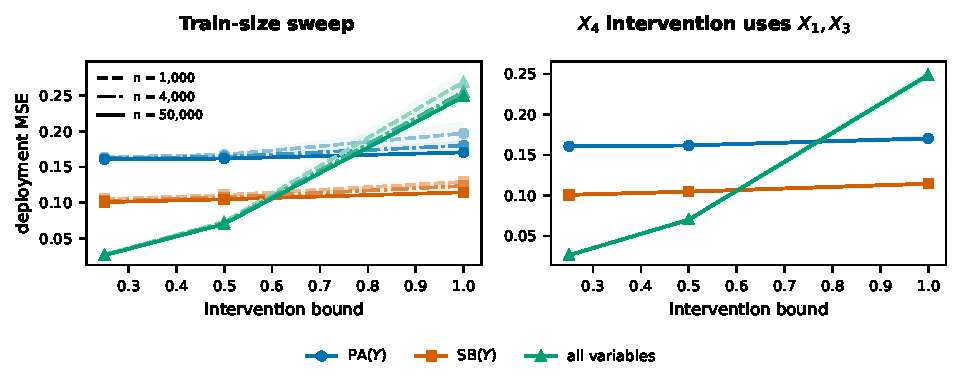
\includegraphics[width=1\linewidth]{images/sweep_and_x4_prediction.pdf}
    \caption{Additional nonlinear SCM results under follower perturbation.
    Left: train-size sweep. 
% \rmj{    for the leader.}
Increasing the leader's sample size ($n \in \{1{,}000, 4{,}000, 50{,}000\}$)
    reduces the residual instability of $\PA(Y)$ and $\SB(Y)$, consistent with a decrease in
    finite-sample regression error. Right: allowing the $X_4$ intervention to
    additionally use $X_1$ and $X_3$ does not qualitatively change the results.}
    \label{fig:synthetic_appendix}
\end{figure}


\subsection{Implementation details of the leader's predictor} \label{app:synthetic_implementation}
 


In the linear-Gaussian SCM, the conditional expectation $\mathbb{E}[Y \given X_S]$ is computed in closed form from the SCM's joint covariance. In the nonlinear SCM, $\hat{f}_S$ is an MLP ($5$ hidden layers of width $256$, ReLU) trained by Adam \citep{kingmaAdamMethodStochastic2015} (learning rate $10^{-3}$, weight decay $10^{-5}$, batch size $512$) on $50{,}000$ training observations, with early stopping determined
%\felix{[seems correct to me]} 
on a $3{,}000$-observation validation set (patience $20$, up to $500$ epochs).
 
Each follower perturbation $E_{\delta_j}$ ($j \in \{1, 4\}$) is an MLP ($2$ hidden layers of width $64$, ReLU) followed by $b \cdot \tanh(\cdot)$ to enforce $|E_{\delta_j}| \leq b$; its inputs are as specified in \Cref{app:dgp}. With $\hat{f}_S$ frozen, $E_{\delta_1}$ and $E_{\delta_4}$ are optimized jointly by Adam (learning rate $10^{-3}$) for $2{,}000$ steps. Each step computes the follower's objective on a fresh batch of $512$ observations
drawn from the SCM with the current $E_{\delta_1}, E_{\delta_4}$ and backpropagates through the SCM forward pass. We use $5$ random restarts and pick the parameters with the best objective value on $10{,}000$ held-out observations.

 
Each curve averages $10$ independent runs with shaded $95\%$ confidence intervals; the reported deployment MSE is computed on $10{,}000$ 
fresh observations under the selected $E_{\delta_1}, E_{\delta_4}$. The experiments are run on an Apple M4 Pro CPU ($14$ cores) using $10$ parallel workers.

% \jonas{[another question one might ask: what if we implement the individual follower here -- do the results change?]} \felix{[ISnt this basically the experiment with additional $X_1$ and $X_3$ information? the follower can choose any conditional distribution (which can also include $X_1$ and $X_3$) which in my opinion is the same as individual followers no?]}
% \jonas{[let's put this on the todo list for a time after we have cleaned up the individual section...]}



\individualexp{\subsection{Comparison with individual followers} \label{app:individual_followers}

The follower in \Cref{sec:synthetic_experiments} is a population follower: its interventions $E_{\delta_1}$ and $E_{\delta_4}$ are functions that apply to the whole population, whereas an individual follower as in \Cref{sec:individuals} chooses an intervention for its own values only.
Here, we compare the two followers empirically in the setting of \Cref{sec:synthetic_experiments}, with one change to the inputs of the population follower that we describe below.
As argued in \Cref{sec:individuals} and \Cref{app:individual_followers_theory}, a population of individual followers is also modeled by a population follower whose interventions depend on the same variables and noise terms, so, when the follower maximizes the MSE, the leader's deployment MSE should be similar under both.
Differences can be due to the training of the population follower's neural network, or to the approximations in computing the individual followers' interventions, which we describe next.

\paragraph{Individual followers.}
We use the SCMs of \Cref{app:dgp} with the graph in \Cref{fig:synthetic_dag}.
An individual follower intervenes only on its own values of $X_1$ and $X_4$, by shifts $\delta_1, \delta_4 \in [-b, b]$ that take the place of $E_{\delta_1}$ and $E_{\delta_4}$.
It chooses $\delta_1$ after observing $(x_2, \varepsilon_1)$, and $\delta_4$ after $Y$ has been realized and it has observed $(x_1, x_2, y, \varepsilon_4)$; it observes neither $x_3$ nor $\varepsilon_5$.
Except for $x_1$, which we discuss below, these are the inputs of $E_{\delta_1}$ and $E_{\delta_4}$ in \Cref{sec:synthetic_experiments}.
The individual knows the SCM and the predictor $f_S$, as the population follower does, and each of its choices maximizes the follower's objective of \Cref{sec:sdfds} given its observations, that is, in expectation over the noise terms it has not observed.

\paragraph{Computation.}
For each of $13$ equally spaced candidate values in $[-b, b]$, we estimate the expected objective that this value leads to by averaging over draws of the unobserved noise terms, and we select the best candidate.
For $\delta_4$, we use $64$ draws of $(\varepsilon_3, \varepsilon_5)$.
For $\delta_1$, the expected objective depends on the later choice of $\delta_4$ (backward induction as in \Cref{app:individual_followers_theory}): for each candidate $\delta_1$, we draw $(\varepsilon_Y, \varepsilon_4)$ $16$ times, compute in each draw the optimal $\delta_4$ and its objective with $16$ draws of $(\varepsilon_3, \varepsilon_5)$, and average.
This grid search is possible because each individual makes only two scalar choices for its own realized inputs, whereas $E_{\delta_1}$ and $E_{\delta_4}$ are functions of their inputs, which \Cref{sec:sdfds} represents by neural networks.
We compute the choices of $4000$ individuals, that is, for $4000$ draws of the exogenous noise, and evaluate the population follower on the same draws.

\paragraph{Information of the two followers.}
In \Cref{sec:synthetic_experiments}, the population follower's $E_{\delta_4}$ depends on $(Y, X_2, \varepsilon_4)$ only, whereas an individual knows $x_1$ when choosing $\delta_4$; with different inputs, the two followers could differ even if both maximized the follower's objective exactly.
In this comparison, $E_{\delta_4}$ therefore depends on $(Y, X_2, \varepsilon_4, X_1)$.
In the notation of \Cref{app:individual_followers_theory}, $O_1 = \{X_2\}$ and $O_4 = \{X_1, X_2, Y\}$, so $A_1 = \varnothing$ and $A_4 = \{X_1\}$, which satisfies the assumption of Lem.~\ref{lem:augmentation}.
This changes the results of \Cref{sec:synthetic_experiments} only slightly: the deployment MSEs of $\PA(Y)$ and $\SB(Y)$ are identical, and those of the all-variable predictor differ by at most $0.002$ ($10$ runs).

\paragraph{Training of the population follower.}
The networks are trained as in \Cref{app:synthetic_implementation}, except that the bound is increased linearly from $0$ to $b$ during the first $1000$ of the $2000$ training steps and equals $b$ afterwards.
The reason is the following.
For the all-variable predictor and a follower maximizing the MSE, the computed optimal shifts of $X_4$ equal $\pm b$ for all individuals, with the sign varying across individuals.
With the full bound from the start, one to three of ten runs end in a local maximum of the follower's objective in which the shift of $X_4$ has the same sign for the whole population; the ramp avoids this.

\individualexp{[TODO for myself: if we use this training recipe, use for all experiments. potentially also add X1 to X4 in 6.1 to harmonize]}

\paragraph{Results.}
\Cref{fig:individual_followers} shows that the leader's deployment MSE under the two followers agrees to within about $1\%$ for $\PA(Y)$ and $\SB(Y)$ under both follower objectives, and for the all-variable predictor when the follower minimizes the prediction $\E[f_S(X_S)]$.
When the follower maximizes the leader's MSE, the individual followers reach a deployment MSE for the all-variable predictor that is less than $1\%$ higher than under the population follower in the linear-Gaussian SCM and $2$ to $5\%$ higher in the nonlinear SCM.
These results suggest that the all-variable curves in \Cref{fig:synthetic_main} slightly underestimate the deployment MSE that an optimal follower achieves.}

\begin{figure}[t]
    \centering
    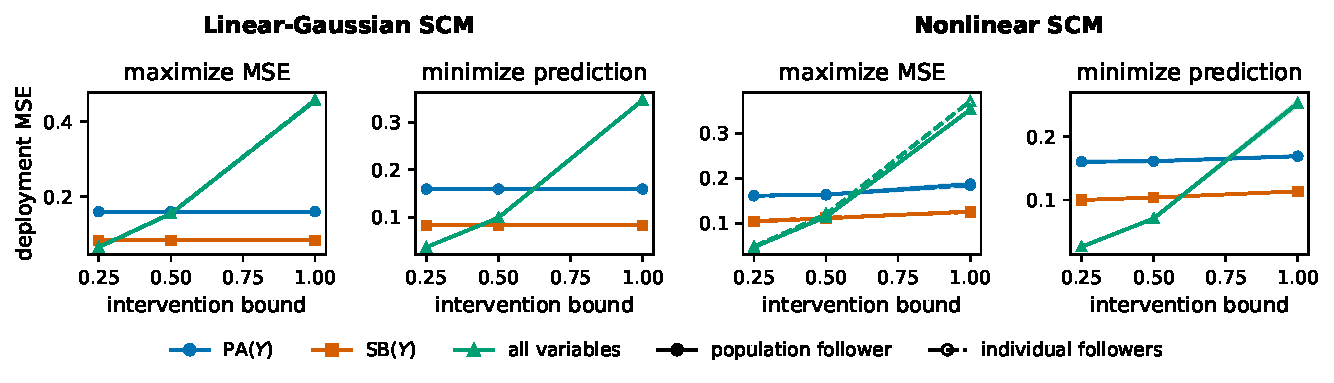
\includegraphics[width=\textwidth]{images/appendix_individual_followers.pdf}
    \caption{\individualexp{Population follower of \Cref{sec:synthetic_experiments} (solid lines, filled markers) and individual followers of \Cref{app:individual_followers} (dashed lines, open markers), evaluated on identical draws of the exogenous noise. For both followers, the intervention on $X_4$ may depend on $X_1$, unlike in \Cref{fig:synthetic_main}.
    Left two panels: linear-Gaussian SCM with population regression predictors.
    Right two panels: nonlinear SCM with predictors estimated from finite data.
    In each pair, the follower maximizes the leader's MSE (left) or minimizes the prediction $\E[f_S(X_S)]$ (right).
    The two followers yield nearly the same deployment MSE for $\PA(Y)$ and $\SB(Y)$ and when the follower minimizes the prediction; when it maximizes the MSE, the individual followers reach a slightly higher deployment MSE for the all-variable predictor.
    Curves average $10$ runs, with $95\%$ confidence bands.}}
    \label{fig:individual_followers}
\end{figure}


\appsection{Additional details for the Causal Chambers experiments} \label{app:additional_details_causal_chambers}


We now provide more details on the experiment described in \cref{sec:new_chamber_experiments}.
We describe the physical device 
and its variables (\Cref{app:causal_chambers_device}), the data-generating process (\Cref{app:causal_chambers_data}), the hidden-confounding hypothesis (\Cref{app:hidden_confounding}), implementation details for predictors deployed by the leader (\Cref{app:implementation_details_leader}), implementation details for the follower (\Cref{app:implementation_details_follower}), and evaluation details (\cref{app:evaluation_causal_chambers}).


\subsection{Causal Chambers: Physical device and variables} \label{app:causal_chambers_device}


We collect data from the Causal Chambers by \citet{gamellaCausalChambersRealworld2025} using the \texttt{causalchamber} API.\footnote{\url{https://github.com/juangamella/causal-chamber-package}} We use the light tunnel \texttt{lt\_mk2\_standard} containing an RGB light source (intensities $\mathtt{red}$, $\mathtt{green}, \mathtt{blue}$), two linear polarizers at adjustable angles ($\mathtt{pol\_1}, \mathtt{pol\_2}$), and three pairs of infrared and visible-light sensors ($\mathtt{ir\_j}$, $\mathtt{vis\_j}$ for $\mathtt{j} \in \{1, 2, 3\}$) at different positions along the tunnel. Sensors at positions $\mathtt{j} = 1, 2$ are unaffected by the polarizers, while sensors at position $\mathtt{j}=3$ are affected by the polarizers through Malus' law.\footnote{The intensity of light passing through both polarizers is proportional to $\cos^2(\mathtt{pol\_1} - \mathtt{pol\_2})$.} An infrared LED placed above the sensors at position $\mathtt{j} = 3$ ($\mathtt{led\_3\_ir}$) activates only during the measurement of $\mathtt{ir\_3}$ and $\mathtt{vis\_3}$, and does not affect the sensors at positions $\mathtt{j} = 1, 2$. \cref{fig:light_tunnel} shows a schematic of the chamber. Tab.~\ref{tab:variables} lists all variables relevant to our experiments. We refer to \citet{gamellaCausalChambersRealworld2025} for the complete documentation.
\begin{figure}[t]
    \centering
    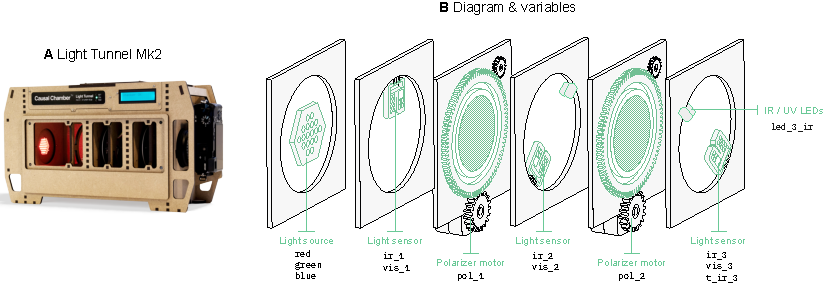
\includegraphics[width=1.0\linewidth]{images/figure_setup_linus_neurips_2026.pdf}
    \caption{Overview of the Causal Chamber light tunnel (\texttt{lt\_mk2\_standard}). (A) Picture of the hardware. (B) Diagram of the hardware components. The displayed variables are relevant for our experiment. We use different subsets of them for classification tasks. Some are not used as covariates but as intervention targets to generate the different environments. Figure adapted from \citet{gamellaCausalChambersRealworld2025}, licensed under CC BY 4.0.}
    \label{fig:light_tunnel}
\end{figure}
\begin{table}[t]
    \centering
    \caption{Causal Chamber light tunnel variables relevant for our experiments. %\jonas{[do we still use pol1 and pol2?]}
    }
    \label{tab:variables}
    \small
    \begin{tabular}{@{}llp{8.5cm}@{}}
        \toprule
        \textbf{Variable} & \textbf{Range} & \textbf{Description} \\
        \midrule
        $\mathtt{red}$, $\mathtt{green}$, $\mathtt{blue}$ & $\{0, \dots, 255\}$
            & Brightness settings for the main light source LEDs. \\
        $\mathtt{ir\_j}$ ($\mathtt{j} \in \{1,2,3\}$) & $[0, 65535]$
            & Uncalibrated infrared intensity measured by sensor at pos.\ $\mathtt{j}$. \\
        $\mathtt{vis\_j}$ ($\mathtt{j} \in \{1,2,3\}$) & $[0, 65535]$
            & Uncalibrated visible-light intensity measured by sensor at pos.\ $\mathtt{j}$. \\
        $\mathtt{pol\_1}$, $\mathtt{pol\_2}$ & $[-270, 270]$
            & Rotation angles for the first and second polarizer (degrees). \\
        $\mathtt{led\_3\_ir}$ & $\{0, \dots, 4095\}$
            & Brightness of the infrared LED placed above sensor at pos.\ $\mathtt{j}=3$. \\
        \bottomrule
    \end{tabular}
\end{table}
\subsection{Data-generating process} \label{app:causal_chambers_data}

The covariate vector is $X = (\mathtt{red},\, \mathtt{green},\, \mathtt{blue},\,  \mathtt{ir\_2},\, \allowbreak \mathtt{vis\_2},\,  \mathtt{ir\_3},\, \mathtt{vis\_3})$. The light intensities are drawn independently from normal distributions truncated to $[0,255] \subseteq \mathbb{R}$, rounded to integers:
\[
    \mathtt{red} \sim \mathcal{N}_{[0,255]}(64, 20^2),\quad
    \mathtt{green} \sim \mathcal{N}_{[0,255]}(32, 30^2),\quad
    \mathtt{blue} \sim \mathcal{N}_{[0,255]}(90, 12^2).
\]
We define $\mathtt{RGB} \coloneq (\mathtt{red}, \mathtt{green}, \mathtt{blue}) \in \mathbb{R}^3$. Data are generated in two stages.
\begin{enumerate}
    \item Target generation: The $\mathtt{RGB}$ values are sampled. The chamber measures the infrared reading $\mathtt{ir\_1}$, and the target is defined as $Y \coloneq \bm{1}\{\mathtt{ir\_1} > \tau\}$, where $\tau = 12{,}500$ corresponds approximately to the median of $\mathtt{ir\_1}$.
 
    \item Downstream interventions: Given the value of $Y$, we intervene on $\mathtt{ir\_3}$ and $\mathtt{vis\_3}$
    % \rmj{(creating spurious \jonas{[do we use this elsewhere in the paper? if so: pls make sure we explain it there]} correlations) by setting}
    by setting
    \[
        \mathtt{led\_3\_ir} \coloneq \beta^{\mathrm{led}}_0 + Y \cdot \beta^{\mathrm{led}}_1,
        \qquad
        \mathtt{pol\_2} \coloneq \beta^{\mathrm{pol}}_0 + Y \cdot \beta^{\mathrm{pol}}_1,
    \]
    rounded to integers in $\{0, \dots, 4095\}$ and $\{0, \ldots, 270\}$, respectively. The coefficients $(\beta^{\mathrm{led}}_0, \beta^{\mathrm{led}}_1, \beta^{\mathrm{pol}}_0, \beta^{\mathrm{pol}}_1)$ vary across environments (Tab.~\ref{tab:interventions_d2}), parameterizing the exogenous variable $E$. The chamber then takes a second round of measurements with these updated settings (the exact values of $\mathtt{RGB}$ from the first stage are kept). Since $\mathtt{led\_3\_ir}$ and $\mathtt{pol\_2}$ influence $\mathtt{ir\_3}$ and $\mathtt{vis\_3}$, this creates an environment-dependent association between $Y$ and the downstream sensor readings at $\mathtt{j}=3$, see \cref{fig:causal_chambers_dags}.
\end{enumerate}
%The causal DAG is shown in \cref{fig:causal_chambers_dags}(b).


Tab.~\ref{tab:interventions_d2} lists the interventions corresponding to the environments. In all three training environments, $\beta^{\mathrm{led}}_0 = \beta^{\mathrm{pol}}_0 = 0$ and $\beta^{\mathrm{led}}_1, \beta^{\mathrm{pol}}_1 \geq 0$, so $Y = 1$ leads to higher (or equal) values of $\mathtt{led\_3\_ir}$ and $\mathtt{pol\_2}$ than $Y = 0$. The effects of $\mathtt{led\_3\_ir}$ (increasing $\mathtt{ir\_3}$) and $\mathtt{pol\_2}$ (decreasing $\mathtt{ir\_3}$ and $\mathtt{vis\_3}$) partially cancel, resulting in a positive correlation between $Y$ and $\mathtt{ir\_3}$, making $\mathtt{ir\_3}$ a highly predictive training feature. A choice of $\beta^{\mathrm{led}}_0, \beta^{\mathrm{pol}}_0 > 0$ and $\beta^{\mathrm{led}}_1, \beta^{\mathrm{pol}}_1 < 0$ by a follower 
%\jonas{[this is an interesting experiment also because we restrict the class of follower's interventions]} \linus{[added below]}
could 
reverse the relationship: $Y = 1$ would yield lower values of $\mathtt{led\_3\_ir}$ and $\mathtt{pol\_2}$. A classifier making predictions based on $\mathtt{ir\_3}$ 
would 
perform badly
% \rmj{encounter a reversed signal}
in such an environment. The follower's intervention class here is more restricted than in
the framework of \Cref{sec:problem_setup}. This makes the experiment a
realistic test of our framework, since in practice followers are typically
limited to a particular set of actions rather than able to intervene
arbitrarily.



% \jonas{[remove next sentence?]}
% The released code generates additional training and test environments; the experiments here 
% use only $E \in \{0, 1, 2\}$ as training environments for the leader.


\begin{table}[t]
    \centering
    \caption{%
      Interventions in different environments. The coefficients $(\beta^{\mathrm{led}}_0, \beta^{\mathrm{led}}_1, \beta^{\mathrm{pol}}_0, \beta^{\mathrm{pol}}_1)$ control the environment-dependent effect of $Y$ on $\mathtt{led\_3\_ir}$ and $\mathtt{pol\_2}$.%
    }
    \label{tab:interventions_d2}
    \small
    \begin{tabular}{@{}clcccc@{}}
        \toprule
        & $E$ & $\beta^{\mathrm{led}}_0$ & $\beta^{\mathrm{led}}_1$
            & $\beta^{\mathrm{pol}}_0$ & $\beta^{\mathrm{pol}}_1$ \\
        \midrule
        %\multirow{6}{*}{\rotatebox{90}{Training}}
        & 0  & 0 & 0 & 0 & 0 \\
        & 1  & 0 & 20 & 0 & 50 \\
        & 2  & 0 & 8 & 0 & 20 \\
        \bottomrule
    \end{tabular}
\end{table}


% \paragraph{Ground-truth invariant subsets.}
% The environment intervenes on $\{\mathtt{red},\, \mathtt{green},\, \mathtt{blue}\}$ and on the relationship between $Y$ and its descendants $\mathtt{led\_3\_ir}$ and $\mathtt{pol\_2}$. Consequently, $\mathtt{ir\_3}$ and $\mathtt{vis\_3}$ are descendants of intervened children of $Y$. The stable blanket is $\SB(Y) = \{\mathtt{red},\, \mathtt{green},\, \mathtt{blue}\}$. The collection of all invariant subsets is
% \[
%     \mathcal{I}_\Env = \bigl\{ \{\mathtt{red},\, \mathtt{green},\, \mathtt{blue}\} \cup T
%     : T \subseteq \{\mathtt{ir\_2},\, \mathtt{vis\_2}\} \bigr\}.
% \]
% Unlike in D-lin and D-nonlin, proper subsets of $\{\mathtt{red},\, \mathtt{green},\, \mathtt{blue}\}$ are not invariant: since $E$ intervenes on individual color channels, omitting any one channel leaves an unblocked path from $E$ to $Y$. The variables $\mathtt{ir\_2}$ and $\mathtt{vis\_2}$ can be freely added.

\subsection{Hidden confounding} \label{app:hidden_confounding}
\citet{gamellaCausalChambersRealworld2025} provide partial causal-graph
information for the light tunnel, where an edge $Z_1 \to Z_2$ means that
intervening on $Z_1$ changes the distribution of subsequent measurements of $Z_2$.
They note that the absence of an edge in their graphs does not preclude a
causal effect or confounding by unmeasured variables.
Under the DAG in \cref{fig:causal_chambers_dags} (middle)\linus{, which} we inferred from their provided information, we would expect conditional independencies of the form $\mathtt{ir\_i} \indep \mathtt{ir\_j} \given \mathtt{RGB}$ and $\mathtt{vis\_i} \indep \mathtt{vis\_j} \given \mathtt{RGB}$ to hold by the global Markov property. Tab.~\ref{tab:hidden_conf} reports $p$-values for the corresponding null hypotheses in the training environments described in \Cref{app:causal_chambers_data}, computed with the weighted GCM test \citep{scheideggerWeightedGeneralisedCovariance2022}. The conditional independencies are rejected in the majority of cases.
We hypothesize that this is because of hidden confounding (such as background lighting) and believe the graph in \cref{fig:causal_chambers_dags} (right) is a more accurate description. Indeed, this is in correspondence with the results presented in \cref{sec:new_chamber_experiments}.
\begin{table}[t]
    \centering
    \caption{%
      $p$-values of a conditional independence test (Weighted GCM test \citep{scheideggerWeightedGeneralisedCovariance2022}) for the null hypothesis $Z_1 \indep Z_2 \given \mathtt{RGB}$. Conditional independence is rejected in the majority of cases, and in particular when pooling the data from all training environments. % \jonas{[one could test pooled over E, no? i would add that (seems natural)]} \linus{[to myself: describe pooled]}
    }
    \label{tab:hidden_conf}
    \small
\begin{tabular}{llrrrr}
\toprule
 & & \multicolumn{4}{c}{$p$-value} \\
\cmidrule(lr){3-6}
$Z_1$ & $Z_2$ & $E=0$ & $E=1$ & $E=2$ & $E \in \{0,1,2\}$ \\
\midrule
$\mathtt{ir\_1}$ & $\mathtt{ir\_2}$ & $<0.001$ & $<0.001$ & $<0.001$ & $<0.001$ \\
$\mathtt{ir\_2}$ & $\mathtt{ir\_3}$ & $<0.001$ & $0.688$ & $<0.001$ & $<0.001$ \\
$\mathtt{vis\_1}$ & $\mathtt{vis\_2}$ & $<0.001$ & $<0.001$ & $<0.001$ & $<0.001$ \\
$\mathtt{vis\_2}$ & $\mathtt{vis\_3}$ & $<0.001$ & $0.081$ & $<0.001$ & $<0.001$ \\
\bottomrule
\end{tabular}
\end{table}




\subsection{Implementation details (leader)} \label{app:implementation_details_leader}


The leader trains five predictors on data pooled from the three training environments $E \in \{0, 1, 2\}$ (Tab.~\ref{tab:interventions_d2}), with $10{,}000$ observations per environment. Four predictors are random forests (\texttt{scikit-learn} \citep{scikit-learn} defaults, $100$ trees) restricted to the covariate subsets indicated by their subscript: $\hat{f}_{\mathtt{RGB}}$, $\hat{f}_{\mathtt{RGB}, \mathtt{ir\_2}}$, $\hat{f}_{\mathtt{RGB}, \mathtt{ir\_2}, \mathtt{vis\_2}}$, and $\hat{f}_\mathrm{all}$. The fifth predictor is the stabilized-classification ensemble $\hat{f}^\mathrm{SC}$ (\Cref{sec:learning_subset_predictors}). All five predictors are held fixed after training.
 
For SC, we use $\alpha_\mathrm{inv} = \alpha_\mathrm{pred} = 0.05$ without tuning, enumerate all $2^d$ ($d=7$) feature subsets, and apply no screening. Predictiveness is scored by out-of-sample binary cross-entropy on the pooled training environments, using out-of-bag predictions; the predictive cutoff is set by $250$ bootstrap samples. Invariance is tested with the \textsc{tram}-GCM test \citep{kookModelbasedCausalFeature2023}, using a Python re-implementation of the non-parametric \texttt{rangerICP} variant ported from the \texttt{tramicp} package \citep{tramicp}. All random forests inside SC (both the base classifiers and those used in the invariance test) use $100$ trees, with \texttt{scikit-learn} defaults.
%\rml{To reduce the cost of the invariance test, $\hat{f}^\mathrm{SC}$ is fit on a subsample of $500$ observations per training environment ($1{,}500$ in total).} 
% \linus{[we fit it now on all data]} 
% \jonas{[either redo or mention in the main text that it is based on less data]}
% \jonas{+1}

All computations run in minutes on an Apple M4 Pro CPU ($14$ cores) using $10$ parallel workers; the dominant cost of the experiment is data collection from the chamber via the API.
 



\subsection{Implementation details (follower)} \label{app:implementation_details_follower}

For a given deployed predictor $\hat{f}$, the follower picks one environment from a fixed candidate set $\Env$ of $49$ environments. We denote this choice by $e^*(\hat{f})$ to emphasize its dependence on $\hat{f}$; different predictors can lead to different choices. Each environment is specified by a coefficient tuple $(\beta^{\mathrm{led}}_0, \beta^{\mathrm{led}}_1, \beta^{\mathrm{pol}}_0, \beta^{\mathrm{pol}}_1)$, as in \Cref{app:causal_chambers_data}. The reference environment $e_\mathrm{ref}$ has coefficients $(0, 12, 0, 30)$; the magnitudes of its slope coefficients lie between those of the training environments $E = 1$ and $E = 2$ (Tab.~\ref{tab:interventions_d2}). The remaining $48$ environments form a $6 \times 8$ grid combining six intensity scales with eight non-trivial sign patterns for the (LED, polarizer) pair: each component takes one of three patterns: switched off, the training pattern (active for $Y = 1$), or reversed (active for $Y = 0$).
 
We order the $49$ environments by their normalized $\ell_\infty$ distance to $e_\mathrm{ref}$ in the slope coefficients $(\beta^{\mathrm{led}}_1, \beta^{\mathrm{pol}}_1)$ (each component normalized by $25$ and $60$, respectively; full definition in the released code). For an intervention bound $b \in [0, 1]$, the choice set $\Env_b \subseteq \Env$ consists of the $\max\{1,\lceil 49 b \rceil\}$ environments closest to $e_\mathrm{ref}$; in particular, we set $\Env_{b=0} \coloneq \{e_\mathrm{ref}\}$.
 
For each candidate environment $e \in \Env_b$, we draw $500$ observations of $X$ from the chamber under $e$. The follower estimates the population mean prediction $\E_e[\hat{f}(X)]$ from these observations and selects the environment $e^*(\hat{f}) \in \Env_b$ minimizing this estimate.


\subsection{Evaluation} \label{app:evaluation_causal_chambers}


After the follower's selection, we draw an independent set of $500$ observations of $X$ from $e^*(\hat{f})$. For each predictor $\hat{f}$ and each value of $b \in \{0, 0.05, 0.1, 0.25, 0.5\}$, we report on this evaluation set two quantities: (i) the shift in the population mean prediction relative to the reference, $\E_{e^*(\hat{f})}[\hat{f}(X)] - \E_{e_\mathrm{ref}}[\hat{f}(X)]$, and (ii) the leader's MSE under the chosen environment, $R_{e^*(\hat{f})}(\hat{f})$. Both are plotted against $b$ in \Cref{fig:follower_chambers}; for reference, the right panel also shows the leader's MSE under $e_\mathrm{ref}$ as a dotted horizontal line for each predictor.


% \appsection{DELETE Experimental details} \label{app:experiment_details}


% {\color{mygreen}

% \linus{We evaluate the approaches presented in \Cref{sec:learning_subset_predictors}. We consider the worst-case risk over a set of fixed test environments. Thus, this setup corresponds to a leader strategy which minimizes the worst-case upper bound \eqref{eq:worst_case_obj}. Alternatively, it corresponds to the case $\Vfoll_e(f) = R_e(f)$ with a limited set of follower interventions. Because stabilized regression and IMP were proposed for continuous responses, we focus on the case  $Y \in \{0,1\}$ and port these methods to classification by changing base models and invariance tests.}

% We use real-world data from the Causal Chambers developed by \citet{gamellaCausalChambersRealworld2025}. These devices are controlled through an API and collect measurements from a physical system with known causal ground-truth. Specifically, we design three datasets to evaluate the following questions: (i) can SC and IMP attain the performance of an oracle method with knowledge of the stable blanket, (ii) do these hard-constraint invariance methods outperform methods using soft penalties, such as IRM, when spurious features dominate the training risk, and (iii) which invariance test is most reliable in combination with SC and IMP? All results are reproducible using the code at \url{link/to/repo/TODO}. \linus{[TODO: anonymous link, add to checklist, maybe at start of section (both experiments)]}

% \paragraph{Datasets.} We use the light tunnel chamber with an RGB light source (intensities $\mathtt{red}$, $\mathtt{green}$, $\mathtt{blue}$), two polarizers ($\mathtt{pol\_1}, \mathtt{pol\_2}$), and infrared and visible-light sensors ($\mathtt{ir\_j}$, $\mathtt{vis\_j}$) at positions $\mathtt{j} \in \{1,2,3\}$. We construct three binary classification tasks, each with $Y \in \{0,1\}$ and $X \in \mathbb{R}^7$ (RGB and four sensor readings). Fig.~\ref{fig:causal_chambers_dags} shows the chamber and the causal DAGs, and Fig.~\ref{fig:light_tunnel} a schematic of the light tunnel. Appendix~\ref{app:causal_chambers_data} describes the data generation and ground-truth invariant subsets in detail.

% \begin{figure}[t]
%     \centering
%     \begin{minipage}{0.25\textwidth}
%         \centering
%         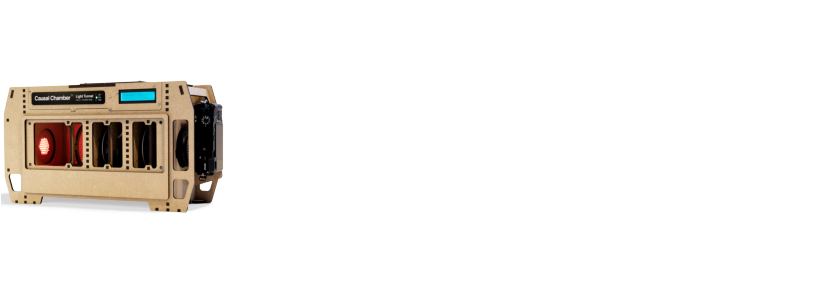
\includegraphics[width=\linewidth]{images/causal_chamber.pdf}
%     \end{minipage}\hfill
%     \begin{minipage}{0.35\textwidth}
%         \centering
%         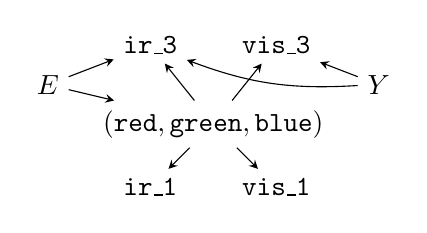
\begin{tikzpicture}[>=stealth, scale=1.0]
    \node (E) at (-2.1, 0.5) {$E$};
    \node (RGB) at (0, 0) {$\mathtt{(red, green, blue)}$};
    \node (Y) at (2.1, 0.5) {$Y$};

    \node (ir3) at (-0.8, 1) {$\mathtt{ir\_3}$};
    \node (vis3) at (0.8, 1) {$\mathtt{vis\_3}$};
    \node (ir1) at (-0.8, -0.8) {$\mathtt{ir\_1}$};
    \node (vis1) at (0.8, -0.8) {$\mathtt{vis\_1}$};

    \draw[->] (Y) to[bend left=12] (ir3);
    \draw[->] (Y) -- (vis3);
    \draw[->] (E) -- (ir3);
    \draw[->] (E) -- (RGB);
    \draw[->] (RGB) -- (ir3);
    \draw[->] (RGB) -- (vis3);
    \draw[->] (RGB) -- (ir1);
    \draw[->] (RGB) -- (vis1);
\end{tikzpicture}
%     \end{minipage} \hfill
%     \begin{minipage}{0.35\textwidth}
%         \centering
%         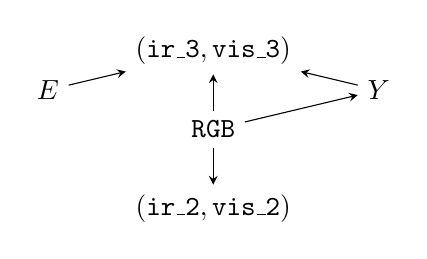
\begin{tikzpicture}[>=stealth, scale=1.0]
    \node (E) at (-2.1, 0.5) {$E$};
    \node (RGB) at (0, 0) {$\mathtt{RGB}$};
    \node (Y) at (2.1, 0.5) {$Y$};
    \node (Bottom) at (0, -1) {$(\mathtt{ir\_2}, \mathtt{vis\_2})$};
    \node (Top) at (0, 1) {$\mathtt{(ir\_3, vis\_3)}$};
    % \node (ir2) at (-0.8, -0.8) {$\mathtt{ir\_2}$};
    % \node (vis2) at (0.8, -0.8) {$\mathtt{vis\_2}$};

    \draw[->] (E) -- (Top);
    % \draw[->] (E) -- (RGB);
    \draw[->] (RGB) -- (Top);
    \draw[->] (RGB) -- (Y);
    \draw[->] (Y) -- (Top);
    \draw[->] (RGB) -- (Bottom);
    %\draw[->] (RGB) -- (vis2);
\end{tikzpicture}
%     \end{minipage}
%     \caption{Causal Chamber light tunnel hardware (left; adapted from \citet{gamellaCausalChambersRealworld2025}, licensed under CC BY 4.0), and causal DAGs for D-nonlin (middle) and D-spur (right). For D-spur, $\mathtt{ir\_3}$ and $\mathtt{vis\_3}$ are grouped as they share the same causal parents.}
%     %\label{fig:causal_chambers_dags}
% \end{figure}

% Dataset D-nonlin (nonlinear): $\mathtt{pol\_1}$ is sampled uniformly from $\{0^\circ, 20^\circ, 30^\circ, 50^\circ\}$ while $\mathtt{pol\_2} = 0$, and we set $Y \coloneq \bm{1}\{\mathtt{pol\_1} \in \{20^\circ, 30^\circ\}\}$. By Malus' law, $\mathtt{vis\_3}$ is proportional to $\cos^2(\mathtt{pol\_1} - \mathtt{pol\_2})$, so the positive class corresponds to intermediate values of $\mathtt{vis\_3}$ and the decision boundary is nonlinear. Environments intervene on the light source and $\mathtt{ir\_3} \in \CH(Y)$. The stable blanket is $\SB(Y) = \{\mathtt{red}, \, \mathtt{green}, \, \mathtt{blue}, \, \mathtt{vis\_3}\}$. We defer an additional dataset, D-lin (linear decision boundary, otherwise similar to D-nonlin), to Appendix~\ref{app:experiment_details}.

% Dataset D-spur (strong spurious correlations): With this dataset, we evaluate whether IMP and SC with their hard invariance constraints can succeed when spurious features are strongly predictive during training. We call a variable spurious if it is in $\DEYforb$. We set $Y \coloneq \bm{1}\{\mathtt{ir\_1} > \tau\}$ for a threshold $\tau$. Environments intervene on RGB and on the sensors $\mathtt{ir\_3}, \mathtt{vis\_3} \in \CH(Y)$. The stable blanket is $\SB(Y) = \{\mathtt{red}, \, \mathtt{green}, \, \mathtt{blue}\}$. On training data, $\mathtt{ir\_3}$ is strongly correlated with $Y$ and more predictive than RGB alone, but this correlation reverses in some test environments.

% \paragraph{Evaluation protocol.}
% We use $|\Envtr| = 6$ training environments with $n_e = 200$ i.i.d.\ observations each, and $5$ unseen test environments per dataset. We report the worst-case (minimum) accuracy over the test environments, averaged over $25$ repetitions with $95\%$ $t$-test confidence intervals. Full details are in Appendix~\ref{app:implementation-details}. Appendix~\ref{app:BCE_results} repeats the evaluation under the binary cross-entropy.

% \paragraph{Methods.}
% We apply SC and IMP with the \textsc{tram}-GCM test \citep{kookModelbasedCausalFeature2023}, which performed well across our settings (comparison with other tests from \Cref{sec:learning_subset_predictors} in Appendix~\ref{app:ensemble_vs_best}). We consider both logistic regression (SC-LR, IMP-LR) and random forests (SC-RF, IMP-RF) for the invariance test and base classifier. We use the defaults $\alpha_\mathrm{inv} = \alpha_\mathrm{pred} = 0.05$ without tuning. We compare against four baselines: pooled empirical risk minimization (ERM-LR, ERM-RF) and Invariant Risk Minimization \citep[IRM;][]{arjovskyInvariantRiskMinimization2020} with a linear model (IRM-Linear) and a multi-layer neural network (IRM-NN). We include oracle methods that fit LR or RF on the ground-truth stable blanket (SB-Oracle-LR, SB-Oracle-RF). Implementation details are in Appendix~\ref{app:implementation-details}.


% \paragraph{Results.} 

% \begin{table}[t]
%   \centering
%   \caption{%
%     Worst-case accuracy over five unseen test environments. SC and IMP both use the \textsc{tram}-GCM test with a logistic regression (LR) or random forest (RF) base classifier. The oracle fits LR or RF on the ground-truth stable blanket. Entries show mean and 95\% $t$-test confidence interval over 25 repetitions. Best non-oracle performance per dataset highlighted in bold. On D-nonlin, IRM-NN achieves the highest accuracy among non-oracle methods. On D-spur, SC and IMP closely match the oracle, while ERM and IRM fail.
%   }
%   \label{tab:main-results}
%   \begin{tabular}{@{}lcc@{}}
%     \toprule
%     Method
%       & {D-nonlin}
%       & {D-spur} \\
%     \midrule
%     \multicolumn{3}{@{}l}{\textbf{Linear methods}} \\[2pt]
%     \quad SC-LR
%       & $0.509 \pm 0.025$ & $\mathbf{0.874 \pm 0.004}$ \\
%     \quad IMP-LR
%       & $0.538 \pm 0.024$ & $0.874 \pm 0.004$ \\
%     \quad ERM-LR
%       & $0.498 \pm 0.035$ & $0.328 \pm 0.010$ \\
%     \quad IRM-Linear
%       & $0.523 \pm 0.032$ & $0.660 \pm 0.078$ \\
%     \quad SB-Oracle-LR
%       & $0.540 \pm 0.018$ & $0.876 \pm 0.001$ \\
%     \midrule
%     \multicolumn{3}{@{}l}{\textbf{Nonlinear methods}} \\[2pt]
%     \quad SC-RF
%       & $0.732 \pm 0.029$ & $0.856 \pm 0.003$ \\
%     \quad IMP-RF
%       & $0.683 \pm 0.030$ & $0.854 \pm 0.003$ \\
%     \quad ERM-RF
%       & $0.685 \pm 0.029$ & $0.315 \pm 0.008$ \\
%     \quad IRM-NN
%       & $\mathbf{0.781 \pm 0.014}$ & $0.320 \pm 0.035$ \\
%     \quad SB-Oracle-RF
%       & $0.788 \pm 0.003$ & $0.856 \pm 0.003$ \\
%   \bottomrule
% \end{tabular}
 
% \end{table}



% Tab.~\ref{tab:main-results} reports the results. The oracle methods establish an upper bound on performance. SC closely matches the oracle on D-spur and approaches it on D-nonlin. IMP performs comparably to SC, except on D-nonlin with random forests. IRM-NN has the highest worst-case accuracy on D-nonlin and the lowest on D-spur among all models. 

% D-nonlin (large gap to oracle): All linear methods including SB-Oracle-LR fail (performance near random guessing). IRM-NN achieves the highest non-oracle worst-case accuracy ($0.781$), followed by SC-RF ($0.732$). The gap between Oracle-RF ($0.788$) and SC is larger than for the other datasets, reflecting that invariance tests are less reliable for nonlinear boundaries (Appendix~\ref{app:test_auc}). Evaluated under the binary cross-entropy, SC achieves the best non-oracle performance (Appendix~\ref{app:BCE_results}). 


% D-spur (SC and IMP succeeds where IRM fails): As expected from the construction of D-spur, methods relying on the spurious features fail: ERM drops to around $0.3$, IRM-Linear to $0.660$, IRM-NN to $0.320$. SC matches the oracle ($0.874$ for LR, $0.856$ for RF) with non-overlapping confidence intervals compared to all baselines. IMP performs comparably to SC. We attribute IRM's failure to its soft invariance penalty being too small relative to the training-loss reduction from including $\mathtt{ir\_3}$ or $\mathtt{vis\_3}$, so the IRM objective favors non-invariant representations even for large penalty weights (Appendix~\ref{app:irm_failure} provides a more detailed analysis). SC and IMP avoid this: subsets containing $\mathtt{ir\_3}$ or $\mathtt{vis\_3}$ are reliably rejected.\footnote{For the \textsc{tram}-GCM test using either LR or RF, not a single subset including $\mathtt{ir\_3}$ or $\mathtt{vis\_3}$ has a $p$-value above 0.05 in all repetitions of the experiment.}


% Appendix~\ref{app:further_experiments} contains additional details and results: full results across all datasets and invariance tests, results under the binary cross-entropy, accuracies in each test environment separately, sensitivity to $n_e$ and to $(\alpha_\mathrm{inv}, \alpha_\mathrm{pred})$, and a comparison of the different invariance tests' ability to separate invariant from non-invariant subsets.
% \linus{[not complete, order]}

% }









% \subsection{Dataset construction} \label{app:causal_chambers_data}

% We construct three datasets from the light tunnel chamber. D-lin and D-nonlin share the same causal graph and stable blanket and differ only in the linearity of the decision boundary. D-spur introduces strongly predictive spurious features that reverse their correlation with the target in some test environments. 


% \subsubsection{Datasets D-lin and D-nonlin} \label{app:datasets_dlin_dnonlin}

% \paragraph{Data-generating process.}
% The covariate vector for D-lin and D-nonlin is $X = (\mathtt{red},\, \mathtt{green},\, \allowbreak \mathtt{blue},\, \mathtt{ir\_1},\, \mathtt{vis\_1},\, \mathtt{ir\_3},\, \mathtt{vis\_3})$. In the reference environment ($E = 0$), the RGB values are drawn independently from normal distributions truncated to $[0,255] \subseteq \mathbb{R}$, rounded to integers:
% \[
%     \mathtt{red} \sim \mathcal{N}_{[0,255]}(100, 25),\quad
%     \mathtt{green} \sim \mathcal{N}_{[0,255]}(80, 20),\quad
%     \mathtt{blue} \sim \mathcal{N}_{[0,255]}(110, 15).
% \]
% All other variables remain at their defaults ($\mathtt{pol\_2} = 0$, $\mathtt{led\_3\_ir} = 0$, $\mathtt{t\_ir\_3} = 3$).
 
% Dataset D-lin: We sample $\mathtt{pol\_1}$ uniformly from $\{0^\circ, 30^\circ\}$ and define $Y \coloneq \bm{1}\{\mathtt{pol\_1} = 30^\circ\}$. The classes are linearly separable with respect to $\mathtt{vis\_3}$.
 
% Dataset D-nonlin: We sample $\mathtt{pol\_1}$ uniformly from $\{0^\circ, 20^\circ, 30^\circ, 50^\circ\}$ and define $Y \coloneq \bm{1}\{\mathtt{pol\_1} \in \{20^\circ, 30^\circ\}\}$. The positive class corresponds to intermediate values of $\mathtt{vis\_3}$, so the decision boundary with respect to $\mathtt{vis\_3}$ is nonlinear.

% D-lin and D-nonlin share the same causal DAG, as shown in \cref{fig:causal_chambers_dags}(a). \cref{fig:scatter_dlin_dnonlin} visualizes the class-conditional densities of $\mathtt{vis\_3}$ in both datasets.
 
% % \begin{figure}[t]
% %   \centering
% %   \includegraphics[width=0.85\linewidth]{images/combined_density_prob_vis3.png}
% %   \caption{%
% %       Class-conditional densities of $\mathtt{vis\_3}$ (shaded) and estimated $\hat{\P}(Y = 1 \given \mathtt{vis\_3})$ (black curve, binned means over 20 quantile bins) for D-lin (left) and D-nonlin (right), pooled across training environments. In D-lin, the conditional probability is monotone and a linear classifier suffices. In D-nonlin, it is non-monotone, requiring a nonlinear decision boundary.%
% % }
% %   \label{fig:scatter_dlin_dnonlin}
% % \end{figure}
 
% \paragraph{Environments and interventions.}
% Environments are created by intervening on the RGB distribution and on $\mathtt{t\_ir\_3}$, the exposure time of sensor $\mathtt{ir\_3}$ (which does not affect $\mathtt{vis\_3}$, as that sensor always uses its default exposure time). There are six training environments and five test environments. Training interventions shift $\mathtt{t\_ir\_3}$ mildly (from the default value of 3 to 2), whereas all test environments apply the stronger shift $\mathtt{t\_ir\_3} = 1$. Hence, $\mathtt{ir\_3}$ is a spurious feature. RGB interventions in the test environments are within or close to the training range but appear in combinations not seen during training. 

 
% % \begin{table}[t]
% %     \centering
% %     \caption{%
% %       Interventions for D-lin and D-nonlin. A dash indicates no intervention (reference distribution). RGB interventions replace the reference distribution with the specified truncated normal $\mathcal{N}_{[0,255]}(\mu, \sigma)$.%
% %     }
% %     \label{tab:interventions_d1}
% %     \small
% %     \begin{tabular}{@{}clcccc@{}}
% %         \toprule
% %         & $E$ & $\mathtt{t\_ir\_3}$ & $\mathtt{red}$ & $\mathtt{green}$ & $\mathtt{blue}$ \\
% %         \midrule
% %         \multirow{6}{*}{\rotatebox{90}{Training}}
% %         & 0 & -- & -- & -- & -- \\
% %         & 1 & 2 & -- & -- & -- \\
% %         & 2 & 2 & $\mathcal{N}_{[0,255]}(130,20)$ & -- & -- \\
% %         & 3 & -- & $\mathcal{N}_{[0,255]}(140,20)$ & -- & -- \\
% %         & 4 & -- & -- & $\mathcal{N}_{[0,255]}(120,25)$ & $\mathcal{N}_{[0,255]}(70,20)$ \\
% %         & 5 & -- & $\mathcal{N}_{[0,255]}(60,20)$ & -- & $\mathcal{N}_{[0,255]}(150,20)$ \\
% %         \midrule
% %         \multirow{5}{*}{\rotatebox{90}{Test}}
% %         & 0 & 1 & -- & -- & -- \\
% %         & 1 & 1 & $\mathcal{N}_{[0,255]}(120,25)$ & -- & -- \\
% %         & 2 & 1 & -- & $\mathcal{N}_{[0,255]}(100,20)$ & -- \\
% %         & 3 & 1 & -- & -- & $\mathcal{N}_{[0,255]}(90,20)$ \\
% %         & 4 & 1 & $\mathcal{N}_{[0,255]}(110,25)$ & $\mathcal{N}_{[0,255]}(90,20)$ & $\mathcal{N}_{[0,255]}(100,20)$ \\
% %         \bottomrule
% %     \end{tabular}
% % \end{table}
 
% \paragraph{Ground-truth invariant subsets.}
% The variable $\mathtt{ir\_3}$ is not part of any invariant subset as it is an intervened child of $Y$. The variable $\mathtt{vis\_3}$ is unaffected by the intervention. The stable blanket is
% $\SB(Y) = \{\mathtt{red},\, \mathtt{green},\, \mathtt{blue},\, \mathtt{vis\_3}\}$.
% % All subsets of $\{\mathtt{red},\, \mathtt{green},\, \mathtt{blue}\}$ (including $\varnothing$) are invariant because $Y$ is determined by $\mathtt{pol\_1}$, which is independent of $E$. The variables $\mathtt{ir\_1}$ and $\mathtt{vis\_1}$ can be freely added to any invariant set because their dependence on $E$ is mediated by $\{\mathtt{red}, \,\mathtt{green}, \,\mathtt{blue}\}$.
% The collection of all invariant subsets is
% \[
%     \mathcal{I}_\Env = \bigl\{ S \cup T : S \in \mathcal{S},\; T \subseteq \{\mathtt{ir\_1}, \mathtt{vis\_1}\} \bigr\},
% \]
% where $\mathcal{S} = 2^{\{\mathtt{red},\mathtt{green},\mathtt{blue}\}} \cup \{\SB(Y)\}$. 



%\subsubsection{Dataset D-spur} \label{app:dataset_dspur}






% \paragraph{Evaluation protocol.}
% For each dataset, we collect data from $|\Envtr| = 6$ training environments ($10{,}000$ observations each) and $5$ unseen test environments in $\Env \setminus \Envtr$ ($5{,}000$ observations each). In each of the $25$ independent repetitions, we draw a subsample of $n_e = 200$ i.i.d.\ observations per training environment, fit all methods, and evaluate on all data from the unseen environments. We report the worst-case (minimum) accuracy over the five unseen environments, averaged over repetitions with $95\%$ $t$-test confidence intervals. 

% \paragraph{Methods.}
% For SC and IMP, we use $\alpha_\mathrm{inv} = \alpha_\mathrm{pred} = 0.05$ without tuning. We enumerate all $2^d$ feature subsets and do not apply pre-screening. Predictiveness is scored by out-of-sample binary cross-entropy on the pooled training environments, using five-fold cross-validation for LR and out-of-bag predictions for RF, and the predictive cutoff uses $250$ bootstrap samples. For the \textsc{tram}-GCM results, we use our own Python implementation of the test, ported from the \texttt{tramicp} R package. Random forests use $500$ trees.

% For IRM we use the gradient-based relaxation IRMv1 \citep{arjovskyInvariantRiskMinimization2020}. IRM-Linear standardizes the inputs and closely follows the implementation by \citet{aubinLinearUnittestsInvariance2021}: a linear predictor wrapped in the original IRM layer with dummy scale and shift parameters, optimized with objective $(1-\lambda)\bar{R} + \lambda\,\mathrm{pen}$, so $\lambda \in [0,1]$ trades off ERM loss and invariance penalty directly. Its grid is learning rate $\{10^{-3}, 5 \cdot 10^{-4}, 10^{-4}\}$, weight decay $\{0, 10^{-4}\}$, penalty weight $\lambda \in \{0.5, 0.7, 0.9, 0.95\}$, and number of iterations $\{5000, 10000\}$. IRM-NN standardizes the inputs and uses an MLP with depth $\{2,3\}$, hidden width $\{16,32\}$, ReLU activations, batch normalization, dropout $\{0,0.1\}$, and a linear output layer. It optimizes the ERM loss plus $\lambda$ times the IRMv1 penalty, with the penalty switched on after $\{50, 100\}$ annealing iterations. Its grid additionally varies the learning rate $\{10^{-3}, 5 \cdot 10^{-4}\}$, weight decay $\{0, 10^{-4}\}$, and penalty weight $\lambda \in \{10, 100, 150, 200\}$. For both IRM baselines, hyperparameters are selected by the worst validation binary cross-entropy on an 80/20 split within each training environment, and the final model is refit on the full training data.

% \paragraph{Computational resources.}
% \linus{[Missing: runtime analysis]}
% \linus{[to myself: TODO]}

% \subsubsection{Runtime analysis} \label{sec:runtime_analysis}

% Tab.~\ref{tab:runtime} reports the runtime for all methods considered in the experiment in \Cref{sec:chamber_experiments}. We consider the same experiment setup as there. Values for IMP are not reported as the fitting is done as during the SC fitting. Runtime for IRM also contains hyperparameter tuning; see \Cref{app:implementation-details}. We measure the runtime on an Apple M4 Pro CPU (14 cores) using 10 parallel workers.


% \subsection{Additional results and analyses} \label{app:further_experiments}

% % {
% % \color{mygreen}

% % Noch versorgen:

% % However, not all SC configurations succeed: for example, SC-IEP-RF ($0.320$) performs as poorly as ERM. \Cref{app:test_auc} confirms that IEP is less reliable at separating invariant from non-invariant subsets on this dataset. The choice of invariance test is therefore important.

% % Among all evaluated invariance tests, SC in combination with the \textsc{tram}-GCM test yields the most robust results across our datasets, also with narrow confidence intervals. We therefore recommend SC-\textsc{tram}-GCM as the default configuration. The choice of base classifier depends on the degree of linearity of the classification problem. 
% % }


% The following sections complement the main results in \Cref{sec:chamber_experiments}. \Cref{app:full_results} reports the results across all three datasets. \Cref{app:test_auc} evaluates the ability of the individual invariance tests to separate invariant from non-invariant subsets. Sections~\ref{app:ensemble_vs_best} and~\ref{app:sample_size} examine the difference between the default ensemble strategy in SC and using only the single best-classifying invariant subset. \Cref{app:hyperparameter_sensitivity} verifies that SC is robust to the choice of $\alpha_\mathrm{inv}$ and $\alpha_\mathrm{pred}$. \Cref{app:irm_failure} explains why IRM fails on D-spur. Sections~\ref{app:per_environment} and ~\ref{app:results_500} report results for each individual test environment and at a larger sample size, respectively. \Cref{app:BCE_results} evaluates SC and baselines in terms of the binary cross-entropy.


% \subsubsection{Results across all datasets} \label{app:full_results}

% Tab.~\ref{tab:main-results-full} extends the main results (Tab.~\ref{tab:main-results}) also to Dataset D-lin (described in \Cref{app:datasets_dlin_dnonlin}). Otherwise, the setup is as in \Cref{sec:chamber_experiments}.

% \begin{table}[t]
%   \centering
%   \caption{%
%     Worst-case accuracy over five unseen test environments on D-lin, D-nonlin, and D-spur. SC and IMP both use the \textsc{tram}-GCM test with a logistic regression (LR) or random forest (RF) base classifier. The oracle fits LR or RF on the ground-truth stable blanket. Entries show mean and 95\% $t$-test confidence interval over 25 repetitions. Best non-oracle performance per dataset highlighted in bold. On D-lin, the differences in performance between the linear models are small. The results for D-nonlin and D-spur appear also in Tab.~\ref{tab:main-results}.
%   }
%   \label{tab:main-results-full}
%   \begin{tabular}{@{}lccc@{}}
%     \toprule
%     Method
%       & {D-lin}
%       & {D-nonlin}
%       & {D-spur} \\
%     \midrule
%     \multicolumn{4}{@{}l}{\textbf{Linear methods}} \\[2pt]
%     \quad SC-LR
%       & $0.909 \pm 0.003$ & $0.509 \pm 0.025$ & $\mathbf{0.874 \pm 0.004}$ \\
%     \quad IMP-LR
%       & $\mathbf{0.910 \pm 0.003}$ & $0.538 \pm 0.024$ & $0.874 \pm 0.004$ \\
%     \quad ERM-LR
%       & $0.878 \pm 0.007$ & $0.498 \pm 0.035$ & $0.328 \pm 0.010$ \\
%     \quad IRM-Linear
%       & $0.890 \pm 0.010$ & $0.523 \pm 0.032$ & $0.660 \pm 0.078$ \\
%     \quad SB-Oracle-LR
%       & $0.912 \pm 0.000$ & $0.540 \pm 0.018$ & $0.876 \pm 0.001$ \\
%     \midrule
%     \multicolumn{4}{@{}l}{\textbf{Nonlinear methods}} \\[2pt]
%     \quad SC-RF
%       & $0.842 \pm 0.031$ & $0.732 \pm 0.029$ & $0.856 \pm 0.003$ \\
%     \quad IMP-RF
%       & $0.836 \pm 0.030$ & $0.683 \pm 0.030$ & $0.854 \pm 0.003$ \\
%     \quad ERM-RF
%       & $0.773 \pm 0.012$ & $0.685 \pm 0.029$ & $0.315 \pm 0.008$ \\
%     \quad IRM-NN
%       & $0.775 \pm 0.063$ & $\mathbf{0.781 \pm 0.014}$ & $0.320 \pm 0.035$ \\
%     \quad SB-Oracle-RF
%       & $0.856 \pm 0.004$ & $0.788 \pm 0.003$ & $0.856 \pm 0.003$ \\
%   \bottomrule
% \end{tabular}
% \end{table}


% On D-lin, all linear methods (including ERM-LR at $0.878$ and IRM-Linear at $0.890$) perform close to SB-Oracle-LR ($0.912$): the stable blanket contains $\mathtt{vis\_3}$, a strong invariant predictor that all methods can access. Linear SC and IMP improve slightly over the baselines (non-overlapping confidence intervals). Hence, even when a strong invariant signal dominates, invariance-based variable selection can provide a small improvement. Nonlinear methods underperform their linear counterparts here. IRM-NN reaches $0.775$ and remains below the
% linear methods: the neural network likely overfits in this low-dimensional, moderate-sample-size
% setting where a linear model already captures the decision boundary well. The results on D-nonlin and on D-spur are discussed in \Cref{sec:chamber_experiments}.







% \subsubsection{Comparison of invariance tests for IMP and SC} \label{app:ensemble_vs_best}

% This section serves two purposes. First, we compare the invariance tests presented in \Cref{sec:learning_subset_predictors} (IRD, \textsc{tram}-GCM, ITP, IEP) in combination with SC and IMP. Second, for each test we contrast the SC ensemble approach (uniform average over classifiers based on subsets in $\hat{\mathcal{C}}_{\Envtr}$) with the single-subset approach IMP that predicts using only $\hat{S}_\mathrm{max} = \argmax_{S \in \hat{\mathcal{I}}_{\Envtr}} s_\mathrm{pred}(S)$. We expect averaging over $\hat{\mathcal{C}}_{\Envtr}$ to reduce variance when the invariance test is unreliable.

% \paragraph{Experimental setup.}
% We evaluate SC and IMP using the invariance tests (IRD, \textsc{tram}-GCM, ITP, IEP) under the same evaluation protocol as \Cref{sec:chamber_experiments}. Each SC and IMP configuration is defined by a base classifier and an invariance test from \Cref{sec:learning_subset_predictors}. We compare linear configurations (invariance test and classifier both based on logistic regression (LR)) and nonlinear configurations (both based on random forests (RF)), yielding configurations such as SC-\textsc{tram}-GCM-RF. 



% We additionally report the rounded mean counts $|\hat{\mathcal{I}}_{\Envtr}|$ (number of subsets found to be invariant) and $|\hat{\mathcal{C}}_{\Envtr}|$ (number of subsets found to be invariant and predictive) for each SC configuration.

% \paragraph{Results.}
% Tab.~\ref{tab:appendix-ensemble-vs-best} reports the worst-case accuracies. Overall, methods based on the \textsc{tram}-GCM test show the most robust performance across all datasets, followed by IRD, which is a bit weaker on D-lin. SC improves over IMP for the random forest base classifier with the largest gains on D-nonlin. Under logistic regression the two strategies perform similarly. On D-nonlin, the linear configurations average over around 60 subsets, substantially more than the nonlinear ones.


% \paragraph{Interpretation.}
% SC improves the most over IMP for random forests on D-nonlin, where the invariance tests are least reliable (\Cref{app:test_auc}). There, averaging dilutes the contribution of non-invariant subsets that pass the invariance filter. On D-lin and D-spur, the invariance filter is already accurate enough that aggregation matters less; for the best SC configurations the ensemble averages over only around five subsets. Not all SC and IMP configurations succeed: for example, SC-IEP-RF ($0.320$) performs as poorly as ERM. \Cref{app:test_auc} confirms that IEP is less reliable at separating invariant from non-invariant subsets on this dataset. The choice of invariance test is therefore important.

% \begin{table}[t]
%   \centering
%   \caption{%
%     SC versus IMP for each invariance test from \Cref{sec:learning_subset_predictors}. Entries show mean and 95\% $t$-test confidence intervals over 25 repetitions with $n_e = 200$ observations per training environment. Numbers in parentheses are the rounded mean counts of subsets in $|\hat{\mathcal{I}}_{\Envtr}|$ and $|\hat{\mathcal{C}}_{\Envtr}|$, respectively. SC improves over IMP in the setting with the random forest base classifier, with the largest gains on D-nonlin. In the setting using logistic regression, the two strategies perform comparably. \textsc{tram}-GCM and IRD perform the most robustly.
%   }
%   \label{tab:appendix-ensemble-vs-best}
%   \small
%   \begin{tabular}{@{}llll@{}}
%     \toprule
%     Method
%       & {D-lin}
%       & {D-nonlin}
%       & {D-spur} \\
%     \midrule
%     \multicolumn{4}{@{}l}{\textbf{Linear methods}} \\[2pt]
%     \quad SC-IRD-LR
%       & $0.894 \pm 0.035$ (37/7) & $0.504 \pm 0.027$ (94/63) & $0.874 \pm 0.004$ (14/6) \\
%     \quad IMP-IRD-LR
%       & $0.895 \pm 0.035$ & $0.538 \pm 0.024$ & $0.873 \pm 0.004$ \\
%     \quad SC-\textsc{tram}-GCM-LR
%       & $0.909 \pm 0.003$ (36/5) & $0.509 \pm 0.025$ (88/60) & $0.874 \pm 0.004$ (13/5) \\
%     \quad IMP-\textsc{tram}-GCM-LR
%       & $0.910 \pm 0.003$ & $0.538 \pm 0.024$ & $0.874 \pm 0.004$ \\
%     \quad SC-ITP-LR
%       & $0.903 \pm 0.007$ (85/9) & $0.482 \pm 0.026$ (102/60) & $0.633 \pm 0.098$ (48/5) \\
%     \quad IMP-ITP-LR
%       & $0.905 \pm 0.008$ & $0.535 \pm 0.024$ & $0.646 \pm 0.098$ \\
%     \midrule
%     \multicolumn{4}{@{}l}{\textbf{Nonlinear methods}} \\[2pt]
%     \quad SC-IRD-RF
%       & $0.824 \pm 0.033$ (42/5) & $0.727 \pm 0.025$ (85/16) & $0.852 \pm 0.007$ (15/6) \\
%     \quad IMP-IRD-RF
%       & $0.794 \pm 0.045$ & $0.679 \pm 0.026$ & $0.850 \pm 0.007$ \\
%     \quad SC-\textsc{tram}-GCM-RF
%       & $0.842 \pm 0.031$ (36/5) & $0.732 \pm 0.029$ (63/11) & $0.856 \pm 0.003$ (13/5) \\
%     \quad IMP-\textsc{tram}-GCM-RF
%       & $0.836 \pm 0.030$ & $0.683 \pm 0.030$ & $0.854 \pm 0.003$ \\
%     \quad SC-ITP-RF
%       & $0.780 \pm 0.029$ (56/4) & $0.737 \pm 0.021$ (73/11) & $0.425 \pm 0.067$ (30/7) \\
%     \quad IMP-ITP-RF
%       & $0.758 \pm 0.029$ & $0.679 \pm 0.027$ & $0.362 \pm 0.053$ \\
%     \quad SC-IEP-RF
%       & $0.756 \pm 0.021$ (116/12) & $0.726 \pm 0.025$ (105/14) & $0.320 \pm 0.007$ (89/35) \\
%     \quad IMP-IEP-RF
%       & $0.764 \pm 0.017$ & $0.682 \pm 0.027$ & $0.317 \pm 0.011$ \\
%   \bottomrule
% \end{tabular}
% \end{table}

% \subsubsection{Discriminative power of invariance tests} \label{app:test_auc}

% Performance differences between SC configurations in \Cref{app:ensemble_vs_best} may reflect differences in how well each invariance test separates invariant from non-invariant subsets. We evaluate this by treating invariance testing as a binary classification problem (``Is a subset invariant or non-invariant?'').

% \paragraph{Experimental setup.}
% For each invariance test and each subset $S$ of covariates, we compute the $p$-value $s_\mathrm{inv}(S)$ using training data from D-lin, D-nonlin, and D-spur (as in \Cref{sec:chamber_experiments}). We then report the area under the ROC curve (AUC) when using these $p$-values to separate invariant from non-invariant subsets, where the binary invariant/non-invariant label is given by the ground-truth $\mathcal{I}_\Env$ derived in \Cref{app:causal_chambers_data}. Results are averaged over 25 random subsamples of $n_e = 200$ observations per training environment. We do not use the test data in this experiment.

% \paragraph{Results.}
% Tab.~\ref{tab:appendix-test-auc} reports the AUC for all tests and datasets. IRD and \textsc{tram}-GCM generally achieve higher AUCs than the other tests. IEP achieves the lowest or near-lowest AUC on every dataset. AUC values are substantially lower across all tests on D-nonlin.

% \begin{table}[t]
%   \centering
%   \caption{%
%     AUC for separating invariant from non-invariant subsets using $p$-values from the invariance tests. Higher AUC indicates that a test more reliably assigns high $p$-values to invariant subsets and low $p$-values to non-invariant subsets. Entries show mean and 95\% $t$-test CI over 25 repetitions with $n_e = 200$ observations per training environment. Best results per dataset in bold. 
%   }
%   \label{tab:appendix-test-auc}
%     \begin{tabular}{@{}lccc@{}}
%     \toprule
%     Method
%       & {D-lin}
%       & {D-nonlin}
%       & {D-spur} \\
%     \midrule
%     %
%     % --- Linear invariance tests -------------------------------------------
%     \multicolumn{4}{@{}l}{\textbf{Linear invariance tests}} \\[2pt]
%     \quad IRD-LR
%       & $\mathbf{0.993 \pm 0.004}$ & $0.718 \pm 0.072$ & $0.959 \pm 0.015$ \\
%     \quad \textsc{tram}-GCM-LR
%       & $0.992 \pm 0.004$ & $0.692 \pm 0.063$ & $0.959 \pm 0.015$ \\
%     \quad ITP-LR
%       & $0.713 \pm 0.055$ & $0.559 \pm 0.070$ & $0.894 \pm 0.026$ \\
%     %
%     \midrule
%     % --- Nonlinear invariance tests ----------------------------------------
%     \multicolumn{4}{@{}l}{\textbf{Nonlinear invariance tests}} \\[2pt]
%     \quad IRD-RF
%       & $0.993 \pm 0.004$ & $0.827 \pm 0.056$ & $\mathbf{0.969 \pm 0.011}$ \\
%     \quad \textsc{tram}-GCM-RF
%       & $0.991 \pm 0.004$ & $\mathbf{0.882 \pm 0.043}$ & $0.969 \pm 0.011$ \\
%     \quad ITP-RF
%       & $0.902 \pm 0.018$ & $0.825 \pm 0.028$ & $0.933 \pm 0.014$ \\
%     \quad IEP-RF
%       & $0.534 \pm 0.022$ & $0.625 \pm 0.023$ & $0.811 \pm 0.038$ \\
%     \bottomrule
%   \end{tabular}
% \end{table}

% \paragraph{Interpretation.}
% The AUC values partially explain the SC performance differences in Tab.~\ref{tab:appendix-ensemble-vs-best}. Tests with higher discriminative AUC, in particular IRD and \textsc{tram}-GCM, generally yield the best SC performance, while IEP, which achieves the lowest AUC on every dataset, produces the worst SC outcomes. The lower AUC levels on D-nonlin are consistent with the larger gap between SC and the oracle on that dataset. However, the AUC as a measure of invariance test performance for our purposes has the limitation that it weights all subsets equally, whereas in practice some non-invariant subsets are more harmful than others. On D-spur, for instance, failing to reject subsets containing $\mathtt{ir\_3}$ is particularly damaging (see Sections~\ref{sec:chamber_experiments},~\ref{app:irm_failure}). We see this in the following two observations. First, on D-spur, even moderate AUC gaps (such as $0.969$ for \textsc{tram}-GCM-RF vs.\ $0.933$ for ITP-RF) can correspond to large drops in SC accuracy ($0.856$ vs.\ $0.425$). Second, on D-nonlin with nonlinear tests, SC accuracies are tightly clustered despite the wider range in AUC, indicating that AUC can only offer partial explanations of SC performance. 

% \subsubsection{Sample-size dependence} \label{app:sample_size}

% \Cref{app:ensemble_vs_best} shows that the advantage of using SC's ensemble approach vs.\ predicting on the single invariant most-predictive (IMP) subset is most pronounced on D-nonlin using random forests. We see in \Cref{app:test_auc}, using also $n_e = 200$ observations per environment, that the invariance tests are less reliable on D-nonlin than on the other datasets. As $n_e$ grows, invariance tests should gain power and the false positive rate of the invariance filter should decrease. We therefore expect the ensemble advantage to diminish and both aggregation strategies to converge as $n_e$ increases.

% \paragraph{Experimental setup.}
% We vary $n_e \in \{50, 100, 200, 300, 500, 750, 1000\}$ for D-nonlin and evaluate SC-\textsc{tram}-GCM-RF. First, we report worst-case accuracies for both the default SC ensemble and using the single best-classifying invariant subset. Further, we report the false positive rate (FPR, fraction of non-invariant subsets with a $p$-value above $\alpha_\mathrm{inv}$) and the true positive rate (TPR, fraction of invariant subsets with $p$-value above $\alpha_\mathrm{inv}$) at the default $\alpha_\mathrm{inv} = 0.05$. Finally, we report the number of subsets in $|\hat{\mathcal{C}}_{\Envtr}|$ that contain the spurious covariate $\mathtt{ir\_3}$. Results are averaged over 100 repetitions.

% \paragraph{Results.}
% \cref{fig:n_e-dependence} shows the results. At small $n_e$, the SC ensemble substantially outperforms IMP. As $n_e$ increases, the gap narrows and the two strategies converge. The worst-case accuracy of the ensemble method first decreases for increasing $n_e$, and increases again for larger $n_e$. The FPR of the invariance testing is substantial for small $n_e$ and decreases monotonically for increasing $n_e$, while the TPR marginally increases and stays above $0.9$. The fraction of subsets in $|\hat{\mathcal{C}}_{\Envtr}|$ that contain the spurious covariate $\mathtt{ir\_3}$ is highest for $n_e \in \{200, 300, 500\}$.

% \begin{figure}[t]
%   \centering
%   \subcaptionbox{Worst-case accuracy.}%
%     {\includegraphics[width=0.49\linewidth]{images/sample_size_d_nonlin_100.pdf}}
%   \hfill
%   \subcaptionbox{FPR and TPR.}%
%     {\includegraphics[width=0.49\linewidth]{images/sample_size_d_nonlin_tpr_fpr_100.pdf}}
  
%   \vspace{1em} % Adjust vertical space between rows as needed

%   \subcaptionbox{Fraction of ensemble members containing $\mathtt{ir\_3}$.}%
%     {\includegraphics[width=0.49\linewidth]{images/sample_size_d_nonlin_ens_ir3_100.pdf}}
  
%   \caption{Effect of $n_e$ on SC-\textsc{tram}-GCM-RF on D-nonlin, averaged over 100 repetitions with 95\% $t$-test confidence bands.
%     (a) Worst-case accuracy for ensemble and best-subset aggregation.
%     (b) FPR and TPR of classifying subsets as invariant/non-invariant using \textsc{tram}-GCM-RF.
%     (c) Fraction of ensemble members that contain the spurious feature $\mathtt{ir\_3}$. The ensemble advantage is largest at small $n_e$ and diminishes as the invariance test becomes more powerful.}
%   \label{fig:n_e-dependence}
% \end{figure}

% \paragraph{Interpretation.}
% The three panels in \cref{fig:n_e-dependence} together explain the non-monotonic behavior of SC's worst-case accuracy. At small $n_e$, the invariance test has a high false positive rate (FPR  around $0.6$), so many non-invariant subsets enter $\hat{\mathcal{C}}_{\Envtr}$. Nevertheless, averaging predictions over many subsets dilutes the influence of any single non-invariant member, and the ensemble substantially outperforms the best-subset strategy. At intermediate $n_e$ (200-500), the invariance filter becomes more selective and $\hat{\mathcal{C}}_{\Envtr}$ smaller, but subsets containing $\mathtt{ir\_3}$ are among the most predictive on the training data and are therefore preferentially retained by the prediction-performance filter whenever they are in $\hat{\mathcal{I}}_{\Envtr}$. This explains the peak in \cref{fig:n_e-dependence}(c). The ensemble thus becomes more concentrated on subsets exploiting the spurious signal, which is the regime where worst-case accuracy is lowest. At large $n_e$ ($\geq 750$), the FPR approaches the nominal $\alpha_\mathrm{inv}$, subsets containing $\mathtt{ir\_3}$ are reliably rejected, and both aggregation strategies converge. Throughout, the TPR stays above $0.9$, confirming that the recovery at large $n_e$ is driven by better rejection of non-invariant subsets rather than by losing invariant ones.


% \subsubsection{Hyperparameter sensitivity} \label{app:hyperparameter_sensitivity}

% SC has two threshold hyperparameters: $\alpha_\mathrm{inv}$ controls the invariance filter (larger values require higher $p$-values, admitting fewer subsets into $\hat{\mathcal{I}}_{\Envtr}$), and $\alpha_\mathrm{pred}$ controls the prediction performance filter (larger values set a higher bootstrap quantile cutoff, admitting fewer subsets into $\hat{\mathcal{C}}_{\Envtr}$). We examine how sensitive SC is to the choice of these parameters. 

% \paragraph{Experimental setup.}
% We vary $\alpha_\mathrm{inv}, \alpha_\mathrm{pred} \in \{0.005, 0.01, 0.05, 0.1, 0.2\}$. We evaluate SC-\textsc{tram}-GCM-RF on all three datasets using the same evaluation protocol as \Cref{sec:chamber_experiments}. Besides the worst-case accuracies, we also report $|\hat{\mathcal{I}}_{\Envtr}|$ and $|\hat{\mathcal{C}}_{\Envtr}|$.


% \paragraph{Results.}
% \cref{fig:hyperparam_heatmap} shows the results. On D-spur, performance is nearly constant across the entire grid (worst-case accuracies between $0.849$ and $0.856$). On D-lin and D-nonlin, the total variation is moderate (total range around $0.05$), but the direction of the gradient differs between the two datasets. On D-lin, performance is highest at small $\alpha_\mathrm{inv}$ (lenient invariance filter, $|\hat{\mathcal{I}}_{\Envtr}| = 41$) and degrades slightly as $\alpha_\mathrm{inv}$ increases. The results barely change with varying $\alpha_\mathrm{pred}$. On D-nonlin, the pattern reverses: performance improves with larger $\alpha_\mathrm{inv}$ (stricter invariance filter, $|\hat{\mathcal{I}}_{\Envtr}|$ decreasing from $81$ to $46$) and with smaller $\alpha_\mathrm{pred}$ (more permissive prediction filter, larger $|\hat{\mathcal{C}}_{\Envtr}|$). The default $\alpha_\mathrm{inv} = \alpha_\mathrm{pred} = 0.05$ lies in a stable region for all three datasets, but is not the single best choice on every dataset.

% \begin{figure}[t]
%   \centering
%   \subcaptionbox{Dataset D-lin.}%
%     {\includegraphics[width=0.49\linewidth]{images/heatmap_d_lin.png}}
%   \hfill
%   \subcaptionbox{Dataset D-nonlin.}%
%     {\includegraphics[width=0.49\linewidth]{images/heatmap_d_nonlin.png}}
  
%   \vspace{1em} 

%   \subcaptionbox{Dataset D-spur.}%
%     {\includegraphics[width=0.49\linewidth]{images/heatmap_d_spur.png}}
  
%   \caption{
%       Sensitivity of SC-\textsc{tram}-GCM-RF to $(\alpha_\mathrm{inv}, \alpha_\mathrm{pred})$ on all three datasets. Each cell shows the mean worst-case accuracy over 25 repetitions, with the rounded mean counts $(|\hat{\mathcal{I}}_{\Envtr}|, |\hat{\mathcal{C}}_{\Envtr}|)$ in parentheses. Larger $\alpha_\mathrm{inv}$ and $\alpha_\mathrm{pred}$ yield stricter filtering and smaller ensembles. Performance is stable across the grid on all datasets (different color scales).
%     }
%   \label{fig:hyperparam_heatmap}
% \end{figure}

% \paragraph{Interpretation.}
% The opposing gradients on D-lin and D-nonlin reflect the different reliability of the invariance test on these datasets. On D-lin, the test separates invariant from non-invariant subsets well (\Cref{app:test_auc}), so a lenient $\alpha_\mathrm{inv}$ admits a large ensemble without introducing many harmful members. On D-nonlin, the test is less reliable, so a lenient threshold lets through non-invariant subsets that hurt worst-case accuracy on the test environments. The effect of $\alpha_\mathrm{pred}$ on D-nonlin is consistent with the ensemble advantage identified in \Cref{app:ensemble_vs_best}: smaller $\alpha_\mathrm{pred}$ yields larger ensembles, which dilute the influence of remaining non-invariant members. On D-spur, the spurious features are reliably rejected across the tested range of $\alpha_\mathrm{inv}$, making performance nearly independent of both hyperparameters. 


% \subsubsection{Failure of IRM on Dataset D-spur} \label{app:irm_failure}

% The objective of Invariant Risk Minimization \citep[IRM;][]{arjovskyInvariantRiskMinimization2020} is to learn a representation $\Phi\colon \mathcal{X} \to \mathcal{H}$ and a classifier $w\colon \mathcal{H} \to [0,1]$ simultaneously, requiring the optimal classifier on top of $\Phi$ to be the same across environments. To solve this computationally difficult optimization problem in practice, the authors propose to directly learn $\Phi: \mathcal{X} \to [0,1]$ by optimizing the relaxed gradient-based objective `IRMv1':
% \begin{equation} \label{eq:IRMv1}
% \sum_{e \in \Envtr} \left( R_e(\Phi) + \lambda \cdot \big( \nabla_{w|w=1} R_e(w \cdot \Phi) \big)^2\right),
% \end{equation}
% where $\lambda$ controls the strength of the invariance penalty. We attribute the failure of IRM on D-spur in \Cref{sec:chamber_experiments} to the IRMv1 penalty. Making the representation $\Phi$ dependent on $\mathtt{ir\_3}$ (or $\mathtt{vis\_3}$) alongside the stable blanket $\{\mathtt{red},\, \mathtt{green},\, \mathtt{blue}\}$ can substantially reduce training risk, while the corresponding increase in the invariance penalty is small relative to this gain. Consequently, the IRM objective \eqref{eq:IRMv1} favors a non-invariant representation even for large penalty parameters $\lambda$. However, in test environments 0 and 3, the correlation between $Y$ and $\mathtt{ir\_3}$ flips. These are precisely the environments where IRM performs worst (see \Cref{app:per_environment}).

% To verify that the IRM objective indeed favors non-invariant supersets of the stable blanket even for large values of $\lambda$, we evaluate it at the ERM optimum for several feature subsets. We evaluate at the ERM optimum because it provides a uniquely defined reference point that isolates the trade-off between training loss and invariance penalty without $\Phi$ itself depending on $\lambda$.


% \paragraph{Experimental setup.}
% We fit a pooled logistic regression model across all training environments on D-spur. To evaluate the penalty term in~\eqref{eq:IRMv1}, we use the pre-sigmoid logit $\Phi(x) = W^\top x + b \in \mathbb{R}$ as the scalar representation: the dummy classifier $w \in \mathbb{R}$ multiplies $\Phi$ before the sigmoid, so $R_e(w \cdot \Phi) = \mathbb{E}_e[\ell(\sigma(w \cdot \Phi(X)),\, Y)]$, where $\ell$ is the binary cross-entropy. The gradient at $w = 1$ then simplifies to
% \[
%     g_e = \nabla_{w|w=1} R_e(w \cdot \Phi)
%         = \mathbb{E}_e\bigl[(\sigma(\Phi(X)) - Y) \cdot \Phi(X)\bigr],
% \]
% and the penalty is $\mathrm{pen} \coloneq \sum_{e \in \Envtr} g_e^2$. We set $R_\mathrm{tr} \coloneq \sum_{e \in \Envtr} R_e(\Phi)$
% %= \sum_{e \in \Envtr} \mathbb{E}_e[\ell(\sigma(\Phi(X^e)),\, Y^e)]$
% and evaluate the reparameterized IRM objective $(1- \lambda) \, R_\mathrm{tr} + \lambda \, \mathrm{pen}$ so that $\lambda \in [0,1]$ directly interpolates between ERM ($\lambda = 0$) and pure invariance enforcement ($\lambda = 1$), making the magnitude of $\lambda$ more interpretable. We limit the available covariates to the stable blanket $\SB(Y) = \{\mathtt{red},\, \mathtt{green},\, \mathtt{blue}\}$, and the non-invariant supersets $\SB(Y) \cup \{\mathtt{ir\_3}\}$ and $\SB(Y) \cup \{\mathtt{vis\_3}\}$, for $\lambda = 0.9$.

% \paragraph{Results.}
% Tab.~\ref{tab:irm_objective} reports the results.
% % training loss $R_\mathrm{tr}$, the invariance penalty $\mathrm{pen}$, and overall IRM objective $(1-\lambda)\,R_\mathrm{tr} + \lambda\,\mathrm{pen}$ for each feature set and $\lambda=0.9$.
% As expected, the IRM penalty is minimized by the stable blanket $\SB(Y)$. Including $\mathtt{ir\_3}$ or $\mathtt{vis\_3}$ substantially reduces the pooled training loss, and this reduction consistently outweighs the corresponding penalty increase. The overall IRM objective is strictly lower for the non-invariant supersets than for $\SB(Y)$ alone, even for the large penalty parameter $\lambda = 0.9$.


% \begin{table}[t]
%   \centering
%   \caption{%
%     IRM objective decomposition on D-spur. Training loss ($R_\mathrm{tr}$), invariance penalty ($\mathrm{pen}$), and overall IRM objective $(1-\lambda)\,R_\mathrm{tr} + \lambda\,\mathrm{pen}$ evaluated at the ERM optimum for three feature sets and $\lambda = 0.9$.
%   }
%   \label{tab:irm_objective}
%   \begin{tabular}{@{}lccc@{}}
%     \toprule
%     Feature set
%       & $R_\mathrm{tr}$
%       & $\mathrm{pen}$
%       & Obj.\ \eqref{eq:IRMv1} ($\lambda=0.9$) \\
%     \midrule
%     $\SB(Y)$ & $0.206$ & $1.002 \times 10^{-4}$ & $0.021$ \\
%     $\SB(Y) \cup \{\mathtt{ir\_3}\}$ & $0.121$ & $5.713 \times 10^{-3}$ & $0.017$ \\
%     $\SB(Y) \cup \{\mathtt{vis\_3}\}$ & $0.137$ & $5.428 \times 10^{-3}$ & $0.019$ \\
%     \bottomrule
%   \end{tabular}
% \end{table}
 
% \paragraph{Interpretation.}
% A relatively large $\lambda > 0.9$ would be necessary to make the stable blanket the global minimizer of the IRM objective. The training loss reduction from including $\mathtt{ir\_3}$ is too large relative to the invariance penalty increase, so the IRM objective prefers the non-invariant superset in our experiment.


% \subsubsection{Per-environment accuracies} \label{app:per_environment}


% \cref{fig:spider} shows the per-environment accuracies of SC-\textsc{tram}-GCM, ERM, IRM, and oracle methods for the experiment in \Cref{sec:chamber_experiments}. On D-lin, the linear methods achieve similar accuracies across the five test environments. A similar pattern holds on D-nonlin for the nonlinear methods. On D-spur, the picture is different: ERM and IRM collapse specifically in test environments 0 and 3, where $\beta^{\mathrm{led}}_1 < 0$ reverses the spurious correlation of $\mathtt{ir\_3}$ with $Y$ (Tab.~\ref{tab:interventions_d2}), while maintaining high accuracy elsewhere. SC-\textsc{tram}-GCM and the oracle remain stable across all five environments. Finally, the gap between SC and the oracle methods observed in \Cref{sec:chamber_experiments} occurs in all environments and not just in the worst one. 

% \begin{figure}[t]
%   \centering
%   \subcaptionbox{Linear methods}%
%     {\includegraphics[width=0.9\linewidth]{images/spider_charts_linear_n200.pdf}}
  
%   \vspace{1em}
  
%   \subcaptionbox{Nonlinear methods}%
%     {\includegraphics[width=0.9\linewidth]{images/spider_charts_nonlinear_n200.pdf}}
%   \caption{Per-environment accuracies on each of the five test environments (described in \Cref{app:causal_chambers_data}) for all three datasets. Top row: linear methods; bottom row: nonlinear methods. On D-lin and D-nonlin, methods perform uniformly across environments when the base classifier matches the decision boundary (linear for D-lin, nonlinear for D-nonlin). On D-spur, ERM and IRM collapse in test environments 0 and 3, where the spurious correlation reverses (\Cref{app:dataset_dspur}), while SC-\textsc{tram}-GCM matches the oracle across all environments.}
%   \label{fig:spider}
% \end{figure}




% \subsubsection{Results at \texorpdfstring{$n_e = 500$}{ne = 500}} \label{app:results_500}

% We repeat the experiment described in \Cref{sec:chamber_experiments} with $n_e = 500$ instead of $n_e = 200$ observations per environment. Tab.~\ref{tab:main-results-500} reports the results. Qualitatively, the main findings from Tab.~\ref{tab:main-results} persist: SC with \textsc{tram}-GCM closely matches the oracle on D-lin and D-spur, ERM and IRM have low worst-case accuracy on D-spur, and IRM-NN shows the best performance on D-nonlin. Confidence intervals are generally narrower than at $n_e = 200$. On D-nonlin, SC does not improve and in fact slightly degrades (such as SC-RF dropping from $0.732$ at $n_e= 200$ to $0.698$) despite the larger sample size, while SB-Oracle-RF improves from $0.788$ to $0.803$, widening the gap. This is consistent with the intermediate-$n_e$ regime identified in \Cref{app:sample_size}, where the invariance filter accepts more subsets containing the spurious covariate $\mathtt{ir\_3}$.

% \begin{table}[t]
%   \centering
%   \caption{%
%     Worst-case accuracy at $n_e = 500$. Setup and notation follow Tab.~\ref{tab:main-results}.
%   }
%   \label{tab:main-results-500}
%   \begin{tabular}{@{}lccc@{}}
%     \toprule
%     Method
%       & {D-lin}
%       & {D-nonlin}
%       & {D-spur} \\
%     \midrule
%     \multicolumn{4}{@{}l}{\textbf{Linear methods}} \\[2pt]
%     \quad SC-LR
%       & $0.911 \pm 0.001$ & $0.515 \pm 0.019$ & $\mathbf{0.877 \pm 0.001}$ \\
%     \quad IMP-LR
%       & $\mathbf{0.911 \pm 0.001}$ & $0.536 \pm 0.020$ & $0.876 \pm 0.001$ \\
%     \quad ERM-LR
%       & $0.886 \pm 0.003$ & $0.503 \pm 0.031$ & $0.313 \pm 0.006$ \\
%     \quad IRM-Linear
%       & $0.901 \pm 0.006$ & $0.535 \pm 0.035$ & $0.637 \pm 0.076$ \\
%     \quad SB-Oracle-LR
%       & $0.912 \pm 0.001$ & $0.560 \pm 0.014$ & $0.877 \pm 0.000$ \\
%     \midrule
%     \multicolumn{4}{@{}l}{\textbf{Nonlinear methods}} \\[2pt]
%     \quad SC-RF
%       & $0.874 \pm 0.003$ & $0.698 \pm 0.042$ & $0.860 \pm 0.004$ \\
%     \quad IMP-RF
%       & $0.870 \pm 0.003$ & $0.673 \pm 0.042$ & $0.857 \pm 0.004$ \\
%     \quad ERM-RF
%       & $0.781 \pm 0.006$ & $0.655 \pm 0.035$ & $0.303 \pm 0.007$ \\
%     \quad IRM-NN
%       & $0.666 \pm 0.072$ & $\mathbf{0.744 \pm 0.013}$ & $0.322 \pm 0.036$ \\
%     \quad SB-Oracle-RF
%       & $0.878 \pm 0.003$ & $0.803 \pm 0.002$ & $0.861 \pm 0.002$ \\
%   \bottomrule
% \end{tabular}
% \end{table}



% \subsubsection{Results for binary cross-entropy} \label{app:BCE_results}

% \Cref{sec:chamber_experiments} evaluates SC and baselines using the worst-case accuracy as an interpretable metric. To align more closely with the theoretical results developed for scoring rules strictly consistent for the mean functional in \Cref{subsec:setting}, we repeat the evaluation using the worst-case binary cross-entropy. The evaluation protocol is identical to \Cref{sec:chamber_experiments}. Lower values now indicate better performance.

% Tab.~\ref{tab:main-results-BCE} shows the results. The findings are qualitatively similar as for Tab.~\ref{tab:main-results}. SC with \textsc{tram}-GCM achieves the best performance among non-oracle methods on all datasets, while ERM and IRM fail on D-spur. On D-spur, the failures are even more pronounced under the binary cross-entropy than the accuracy, because the cross-entropy heavily penalizes wrong but confident predictions, which the accuracy metric does not capture. The most notable difference compared to Tab.~\ref{tab:main-results} concerns D-nonlin: IRM-NN, which achieved the highest worst-case accuracy, now performs worse under cross-entropy ($0.762 \pm 0.248$), while SC-RF achieves the best non-oracle performance ($0.504 \pm 0.015$). This suggests that IRM-NN produces sufficiently correct class labels for high accuracy but poorly calibrated probability estimates. The large confidence interval of IRM-NN on D-nonlin ($\pm 0.248$) further indicates that its predictions are highly unstable across repetitions.


% \begin{table}[t]
%   \centering
%   \caption{%
%     Worst-case binary cross-entropy. Setup and notation follow Tab.~\ref{tab:main-results}; lower values indicate better performance. 
%   }
%   \label{tab:main-results-BCE}
%   \begin{tabular}{@{}lccc@{}}
%     \toprule
%     Method
%       & {D-lin}
%       & {D-nonlin}
%       & {D-spur} \\
%     \midrule
%     \multicolumn{4}{@{}l}{\textbf{Linear methods}} \\[2pt]
%     \quad SC-LR
%       & $0.219 \pm 0.008$ & $0.670 \pm 0.001$ & $0.280 \pm 0.008$ \\
%     \quad IMP-LR
%       & $\mathbf{0.218 \pm 0.008}$ & $0.670 \pm 0.001$ & $\mathbf{0.280 \pm 0.008}$ \\
%     \quad ERM-LR
%       & $0.305 \pm 0.017$ & $0.673 \pm 0.002$ & $3.381 \pm 0.130$ \\
%     \quad IRM-Linear
%       & $0.274 \pm 0.021$ & $0.676 \pm 0.003$ & $1.205 \pm 0.431$ \\
%     \quad SB-Oracle-LR
%       & $0.213 \pm 0.001$ & $0.668 \pm 0.001$ & $0.272 \pm 0.002$ \\
%     \midrule
%     \multicolumn{4}{@{}l}{\textbf{Nonlinear methods}} \\[2pt]
%     \quad SC-RF
%       & $0.350 \pm 0.030$ & $\mathbf{0.504 \pm 0.015}$ & $0.326 \pm 0.005$ \\
%     \quad IMP-RF
%       & $0.372 \pm 0.030$ & $0.545 \pm 0.017$ & $0.360 \pm 0.012$ \\
%     \quad ERM-RF
%       & $0.499 \pm 0.018$ & $0.541 \pm 0.015$ & $2.292 \pm 0.097$ \\
%     \quad IRM-NN
%       & $1.248 \pm 0.575$ & $0.762 \pm 0.248$ & $2.707 \pm 0.353$ \\
%     \quad SB-Oracle-RF
%       & $0.358 \pm 0.014$ & $0.471 \pm 0.014$ & $0.343 \pm 0.004$ \\
%   \bottomrule
% \end{tabular}
% \end{table}





% \begin{table}[t]
%   \centering
%   \caption{%
%    Runtime on D-nonlin in seconds for the experiment in \Cref{sec:chamber_experiments}, averaged over 25 repetitions. 
%   }
  
% \begin{tabular}{@{}lc@{}}
%     \toprule
%     Method
%       & {Runtime (s)} \\
%     \midrule
%     \multicolumn{2}{@{}l}{\textbf{Linear methods}} \\[2pt]
%     \quad SC-LR
%       & $19.434 \pm 0.137$ \\
%     \quad ERM-LR
%       & $0.006 \pm 0.000$ \\
%     \quad IRM-Linear
%       & $24.910 \pm 0.607$ \\
%     \quad SB-Oracle-LR
%       & $0.005 \pm 0.000$ \\
%     \midrule
%     \multicolumn{2}{@{}l}{\textbf{Nonlinear methods}} \\[2pt]
%     \quad SC-RF
%       & $28.041 \pm 0.347$ \\
%     \quad ERM-RF
%       & $0.097 \pm 0.002$ \\
%     \quad IRM-NN
%       & $7.968 \pm 0.411$ \\
%     \quad SB-Oracle-RF
%       & $0.104 \pm 0.007$ \\
%   \bottomrule
% \end{tabular}
%   \label{tab:runtime}
  
% \end{table}






 


% \paragraph{Predictor-specific follower on D-spur.}
% We add one experiment on D-spur that directly implements a finite
% prediction-intervention game. In this experiment the causal graph is treated as
% known. We compare two random forest classifiers: an oracle stable-blanket
% predictor
% \[
%     \hat f_{\mathrm{SB}}(R),
%     \qquad
%     R \coloneqq
%     (\mathtt{red},\mathtt{green},\mathtt{blue}),
% \]
% and a pooled all-variable predictor
% \[
%     \hat f_{\mathrm{all}}(R,B,Z),
%     \qquad
%     B \coloneqq (\mathtt{ir\_2},\mathtt{vis\_2}),
%     \quad
%     Z \coloneqq (\mathtt{ir\_3},\mathtt{vis\_3}).
% \]
% Both predictors are trained on the original D-spur training data. For D-spur,
% the stable blanket is \(R\), while \(Z\) consists of downstream spurious
% features.

% The follower observes the deployed predictor \(f\) and the RGB values \(R\).
% It does not observe \(Y\) when choosing its response. The response is a
% downstream coefficient mechanism
% \[
%     \theta
%     =
%     (\beta^{\mathrm{led}}_0,\beta^{\mathrm{led}}_1,
%       \beta^{\mathrm{pol}}_0,\beta^{\mathrm{pol}}_1).
% \]
% After \(\theta\) has been chosen, the chamber sets
% \begin{equation}
%     \mathtt{led\_3\_ir}
%     =
%     \beta^{\mathrm{led}}_0
%     +
%     Y \beta^{\mathrm{led}}_1,
%     \qquad
%     \mathtt{pol\_2}
%     =
%     \beta^{\mathrm{pol}}_0
%     +
%     Y \beta^{\mathrm{pol}}_1,
%     \label{eq:dspur_follower_mechanism}
% \end{equation}
% and then measures \(B\) and \(Z\). Thus the follower chooses the coefficients
% using only \(R\), but the chosen downstream mechanism contains \(Y\) as an
% existing parent, as in the D-spur construction. This should be read as a
% mechanism-level response, not as an individual who observes \(Y\) before acting.

% The follower wants to lower the predicted positive-class score. We therefore use
% \[
%     \Vfoll_{e_\pi}(f)
%     =
%     - \E_{e_\pi}[f(X)],
% \]
% with no intervention cost.

% \paragraph{Finite set of downstream mechanisms.}
% We use a finite set \(\Theta\) of downstream coefficient mechanisms. The
% reference mechanism is
% \[
%     \theta_0=(0,0,0,0).
% \]
% We also consider two strengths, \(s\in\{0.5,1.0\}\). For these strengths, set
% \[
%     (L_{0.5},P_{0.5})=(12,30),
%     \qquad
%     (L_1,P_1)=(25,60),
% \]
% where \(L_s\) is the LED level and \(P_s\) is the polarizer level used at
% strength \(s\).

% For each strength \(s\), the LED coefficients
% \((\beta^{\mathrm{led}}_0,\beta^{\mathrm{led}}_1)\) are chosen from
% \[
%     (0,0) \quad \text{(off)}, \qquad
%     (0,L_s) \quad \text{(positive)}, \qquad
%     (L_s,-L_s) \quad \text{(reversed)}.
% \]
% Here ``positive'' means that \(Y=1\) gives a larger value of
% \(\mathtt{led\_3\_ir}\) than \(Y=0\), while ``reversed'' means that
% \(Y=1\) gives a smaller value. Similarly, the polarizer coefficients
% \((\beta^{\mathrm{pol}}_0,\beta^{\mathrm{pol}}_1)\) are chosen from
% \[
%     (0,0) \quad \text{(off)}, \qquad
%     (0,P_s) \quad \text{(positive)}, \qquad
%     (P_s,-P_s) \quad \text{(reversed)}.
% \]
% For a fixed strength \(s\), we combine one LED choice with one polarizer choice.
% This gives \(3\times 3=9\) coefficient mechanisms. The all-off mechanism
% \((0,0,0,0)\) is the same for both strengths and is already included as
% \(\theta_0\), so each strength contributes eight new mechanisms. Hence
% \[
%     |\Theta| = 1 + 8 + 8 = 17.
% \]
% This set contains the strongest positive-feedback training mechanism
% \[
%     (0,25,0,60),
% \]
% and the reversed test mechanism from D-spur test environment \(0\),
% \[
%     (25,-25,60,-60).
% \]
% For a mechanism budget \(b\in\{0,0.5,1.0\}\), let
% \[
%     \Theta_b \coloneqq \{\theta\in\Theta:\mathrm{strength}(\theta)\le b\}.
% \]

% \paragraph{Data collection.}
% We collect \(N=2400\) new D-spur samples. First, we sample RGB values from the
% reference D-spur distribution,
% \[
%     \mathtt{red}\sim \mathcal N_{[0,255]}(64,20),
%     \qquad
%     \mathtt{green}\sim \mathcal N_{[0,255]}(32,30),
%     \qquad
%     \mathtt{blue}\sim \mathcal N_{[0,255]}(90,12),
% \]
% rounded to integers. In the first chamber phase, we set these RGB values,
% measure \(\mathtt{ir\_1}\), and define
% \[
%     Y_i = \bm{1}\{\mathtt{ir\_1}_i > 12500\}.
% \]
% In the second chamber phase, we keep the same RGB values and run one experiment
% for each \(\theta_m\in\Theta\). In experiment \(m\), the chamber applies
% \eqref{eq:dspur_follower_mechanism} and records
% \[
%     B_i^{(m)}=(\mathtt{ir\_2}^{(m)},\mathtt{vis\_2}^{(m)}),
%     \qquad
%     Z_i^{(m)}=(\mathtt{ir\_3}^{(m)},\mathtt{vis\_3}^{(m)}).
% \]
% Thus, for every \(i\), we obtain
% \[
%     \left(
%     R_i,\,
%     Y_i,\,
%     \{B_i^{(m)},Z_i^{(m)}\}_{m=1}^{|\Theta|}
%     \right).
% \]
% We split these data into a probe split and an evaluation split of equal size.

% \paragraph{Computing the follower response.}
% The follower may choose different mechanisms for different RGB regions, but we
% keep the class of such responses small. We first compute the RGB-only score
% \[
%     g_{\mathrm{RGB}}(R) \coloneqq \hat f_{\mathrm{SB}}(R).
% \]
% On the probe split, we split the observations into three groups according to the
% tertiles of \(g_{\mathrm{RGB}}(R)\). Let \(T(R)\in\{0,1,2\}\) denote the group
% of \(R\). This grouping is used only to define the finite response class. The
% deployed predictor is still \(f\), which may be either \(\hat f_{\mathrm{SB}}\)
% or \(\hat f_{\mathrm{all}}\).

% For each deployed predictor \(f\), budget \(b\), group \(t\), and mechanism
% \(\theta_m\in\Theta_b\), we estimate on the probe split
% \[
%     \widehat m_f(t,m)
%     =
%     \frac{1}{|\{i:T(R_i)=t\}|}
%     \sum_{i:T(R_i)=t}
%     f\!\left(R_i,B_i^{(m)},Z_i^{(m)}\right).
% \]
% The follower's estimated response is
% \[
%     \hat\pi_f^b(t)
%     \in
%     \argmin_{m:\,\theta_m\in\Theta_b}
%     \widehat m_f(t,m).
% \]
% Thus each deployed predictor gets its own response.

% \paragraph{Evaluation.}
% On the evaluation split, each observation \(i\) is assigned the mechanism chosen
% for its RGB group:
% \[
%     m_i = \hat\pi_f^b(T(R_i)).
% \]
% We then evaluate \(f\) on
% \[
%     X_i^{\hat\pi_f^b}
%     =
%     \left(R_i,B_i^{(m_i)},Z_i^{(m_i)}\right).
% \]
% For each predictor and budget, we report the Brier score, binary
% cross-entropy, the follower objective \(\E[f(X)]\), and the false-negative rate.
% The clean reference is always the no-feedback mechanism \(\theta_0=(0,0,0,0)\).
% We also plot the evaluation-split values of \(\E[f(X)]\) and the Brier score as
% functions of the mechanism budget \(b\).


% We initially allowed the follower to choose different mechanisms in different
% RGB-score groups. In this experiment, the selected mechanisms were almost
% identical across groups, so the results are essentially the same for one, three,
% or more groups. We therefore report the simpler population-level response.







% \appsection{Additional material} \label{app:additional_material}


% \begin{figure}[t]
% \centering
% \begin{tikzpicture}[>={Stealth[round]}, scale = 0.8, every legend/.append style={at={(0,-1.5)}, anchor=north, column sep=1cm}]
    % Define the nodes at specific coordinates
    \node (a1) at (-3, 3) [draw, circle, minimum size=0.96cm] {$X_1$};
    \node (a2) at (3, 0) [draw, circle, minimum size=0.96cm] {$X_2$};
    \node (a3) at (-3, 0) [draw, circle, minimum size=0.96cm] {$X_3$};
    \node (a4) at (-1.5, 1.5) [draw, circle, minimum size=0.96cm] {$X_4$};
    \node (a5) at (1.5, 1.5) [draw, circle, minimum size=0.96cm] {$X_5$};
    \node (a6) at (1.5, -1.5) [draw, circle, minimum size=0.96cm] {$X_6$};
    \node (a7) at (-1.5, -1.5) [draw, circle, minimum size=0.96cm] {$X_7$};
    \node (a8) at (-3, -3.1) [draw, circle, minimum size=0.96cm] {$X_8$};
    \node (aY) at (0, 0) [draw, circle, minimum size=0.96cm,fill=gray!50] {$Y$};
    \node (aE) at (0, -3.1) [draw, circle, minimum size=0.96cm,fill=gray!50] {$E$};
   

    % Define the edges
    \draw[->] (a1) -- (a4);
    \draw[->] (a4) -- (aY);
    \draw[->] (a4) -- (a5);
    \draw[->] (a5) -- (aY);
    \draw[->] (aY) -- (a7);
    \draw[->] (aY) -- (a6);
    \draw[->] (a2) -- (a6);
    \draw[->] (a7) -- (a8);
    \draw[->] (a3) -- (a7);
    \draw[->, line width=0.6mm] (aE) -- (a7);
    \draw[->, line width=0.6mm] (aE) -- (a6);
    \draw[->, line width=0.6mm] (aE) -- (a5);



\begin{pgfonlayer}{background}



%\node[draw, ellipse, color=blue, fill=blue!50, minimum height=1.3cm, minimum width=2cm, opacity=0.2, fit=(a2) (a3) (a4) (a5) (a7), inner sep = -7pt] {};

\node[draw, ellipse, color=blue, fill=blue!50, minimum height=1.4cm, minimum width=2cm, opacity=0.2, fit=(a2) (a3) (a4) (a5) (a7), inner sep = -6pt] at (0,0.05) {};

\node[draw, ellipse, color=green, fill=green!70, minimum height=1.1cm, minimum width=2cm, opacity=0.5, fit=(a4) (a5), inner sep = 1pt] {};

\node[draw, ellipse, color=red, fill=red!50, minimum height=1.1cm, minimum width=1.9cm, opacity=0.6, fit=(a4) (a5), inner sep = -1pt] {};
 
    \end{pgfonlayer}
   




\begin{scope}[shift={(0,-8)}]
       \node (a1) at (-3, 3) [draw, circle, minimum size=0.96cm] {$X_1$};
    \node (a2) at (3, 0) [draw, circle, minimum size=0.96cm] {$X_2$};
    \node (a3) at (-3, 0) [draw, circle, minimum size=0.96cm] {$X_3$};
    \node (a4) at (-1.5, 1.5) [draw, circle, minimum size=0.96cm] {$X_4$};
    \node (a5) at (1.5, 1.5) [draw, circle, minimum size=0.96cm] {$X_5$};
    \node (a6) at (1.5, -1.5) [draw, circle, minimum size=0.96cm] {$X_6$};
    \node (a7) at (-1.5, -1.5) [draw, circle, minimum size=0.96cm] {$X_7$};
    \node (a8) at (-3, -3.1) [draw, circle, minimum size=0.96cm] {$X_8$};
    \node (aY) at (0, 0) [draw, circle, minimum size=0.96cm,fill=gray!50] {$Y$};
    \node (aE) at (0, -3.1) [draw, circle, minimum size=0.96cm,fill=gray!50] {$E$};
   

    % Define the edges
    \draw[->] (a1) -- (a4);
    \draw[->] (a4) -- (aY);
    \draw[->] (a4) -- (a5);
    \draw[->] (a5) -- (aY);
    \draw[->] (aY) -- (a7);
    \draw[->] (aY) -- (a6);
    \draw[->] (a2) -- (a6);
    \draw[->] (a7) -- (a8);
    \draw[->] (a3) -- (a7);
    \draw[->, line width=0.6mm] (aE) -- (a6);
    \draw[->, line width=0.6mm] (aE) -- (a5);



\begin{pgfonlayer}{background}

\node[draw, ellipse, color=blue, fill=blue!50, minimum height=1.4cm, minimum width=2cm, opacity=0.2, fit=(a2) (a3) (a4) (a5) (a7), inner sep = -6pt] at (0,0.05) {};

\node[draw, ellipse, color=green, fill=green!70, minimum height=3.3cm, minimum width=5.1cm, opacity=0.5, inner sep=-5pt, rotate=30] at (-0.8, 0.23) {};


 \node[draw, ellipse, color=red, fill=red!50, minimum height=1.1cm, minimum width=1.9cm, opacity=0.6, fit=(a4) (a5), inner sep = -1pt] {};

 
    \end{pgfonlayer}
    \end{scope}



    \begin{scope}[shift={(0,-16)}]
       \node (a1) at (-3, 3) [draw, circle, minimum size=0.96cm] {$X_1$};
    \node (a2) at (3, 0) [draw, circle, minimum size=0.96cm] {$X_2$};
    \node (a3) at (-3, 0) [draw, circle, minimum size=0.96cm] {$X_3$};
    \node (a4) at (-1.5, 1.5) [draw, circle, minimum size=0.96cm] {$X_4$};
    \node (a5) at (1.5, 1.5) [draw, circle, minimum size=0.96cm] {$X_5$};
    \node (a6) at (1.5, -1.5) [draw, circle, minimum size=0.96cm] {$X_6$};
    \node (a7) at (-1.5, -1.5) [draw, circle, minimum size=0.96cm] {$X_7$};
    \node (a8) at (-3, -3.1) [draw, circle, minimum size=0.96cm] {$X_8$};
    \node (aY) at (0, 0) [draw, circle, minimum size=0.96cm,fill=gray!50] {$Y$};
    \node (aE) at (0, -3.1) [draw, circle, minimum size=0.96cm,fill=gray!50] {$E$};
   

    % Define the edges
    \draw[->] (a1) -- (a4);
    \draw[->] (a4) -- (aY);
    \draw[->] (a4) -- (a5);
    \draw[->] (a5) -- (aY);
    \draw[->] (aY) -- (a7);
    \draw[->] (aY) -- (a6);
    \draw[->] (a2) -- (a6);
    \draw[->] (a7) -- (a8);
    \draw[->] (a3) -- (a7);
    \draw[->, line width=0.6mm] (aE) -- (a5);




\begin{pgfonlayer}{background}

\node[draw, ellipse, color=blue, fill=blue!50, minimum height=1.4cm, minimum width=2cm, opacity=0.2, fit=(a2) (a3) (a4) (a5) (a7), inner sep = -6pt] at (0,0.05) {};

        \node[draw, ellipse, color=green, fill=green!70, minimum height=1.4cm, minimum width=2cm, opacity=0.5, fit=(a2) (a3) (a4) (a5) (a7), inner sep = -9pt] at (0,0.05) {};

 \node[draw, ellipse, color=red, fill=red!50, minimum height=1.1cm, minimum width=1.9cm, opacity=0.6, fit=(a4) (a5), inner sep = -1pt] {};



 
 
    \end{pgfonlayer}
    \end{scope}


% Legend
    \begin{scope}[shift={(0,-21)}]
        \node (legend) [rectangle, draw, fill=white, opacity=0.5, text opacity=1, inner sep=1em] {
            \begin{tabular}{@{}ccc@{}}
                \textcolor{red!40}{\rule{0.6cm}{0.3cm}} $\PA(Y)$ & \textcolor{green!40}{\rule{0.6cm}{0.3cm}} $\SB(Y)$ & \textcolor{blue!20}{\rule{0.6cm}{0.3cm}} $\MB(Y)$ 
            \end{tabular}
        };
    \end{scope}


    
    
\end{tikzpicture}
% \vspace{15px}
% \caption{
% %\linus{[fig commented out for faster compilation]} 
% Change of the stable blanket with the number of interventions. The stable blanket is minimal ($\SB(Y) = \PA(Y)$) for three interventions at the top, of intermediate size ($\PA(Y) \subsetneq \SB(Y) \subsetneq \MB(Y)$) for two interventions in the middle, and maximal ($\SB(Y) = \MB(Y)$) for one intervention. The figure extends Fig.~4 by \citet{pfisterStabilizingVariableSelection2021}.}
% \label{fig:PA_SB_MB}
% \end{figure}



\newpage
\section*{NeurIPS Paper Checklist}

%%% BEGIN INSTRUCTIONS %%%
% The checklist is designed to encourage best practices for responsible machine learning research, addressing issues of reproducibility, transparency, research ethics, and societal impact. Do not remove the checklist: {\bf The papers not including the checklist will be desk rejected.} The checklist should follow the references and follow the (optional) supplemental material.  The checklist does NOT count towards the page
% limit. 

% Please read the checklist guidelines carefully for information on how to answer these questions. For each question in the checklist:
% \begin{itemize}
%     \item You should answer \answerYes{}, \answerNo{}, or \answerNA{}.
%     \item \answerNA{} means either that the question is Not Applicable for that particular paper or the relevant information is Not Available.
%     \item Please provide a short (1--2 sentence) justification right after your answer (even for \answerNA). 
%    % \item {\bf The papers not including the checklist will be desk rejected.}
% \end{itemize}

% {\bf The checklist answers are an integral part of your paper submission.} They are visible to the reviewers, area chairs, senior area chairs, and ethics reviewers. You will also be asked to include it (after eventual revisions) with the final version of your paper, and its final version will be published with the paper.

% The reviewers of your paper will be asked to use the checklist as one of the factors in their evaluation. While \answerYes{} is generally preferable to \answerNo{}, it is perfectly acceptable to answer \answerNo{} provided a proper justification is given (e.g., error bars are not reported because it would be too computationally expensive'' or ``we were unable to find the license for the dataset we used''). In general, answering \answerNo{} or \answerNA{} is not grounds for rejection. While the questions are phrased in a binary way, we acknowledge that the true answer is often more nuanced, so please just use your best judgment and write a justification to elaborate. All supporting evidence can appear either in the main paper or the supplemental material, provided in appendix. If you answer \answerYes{} to a question, in the justification please point to the section(s) where related material for the question can be found.

% IMPORTANT, please:
% \begin{itemize}
%     \item {\bf Delete this instruction block, but keep the section heading ``NeurIPS Paper Checklist"},
%     \item  {\bf Keep the checklist subsection headings, questions/answers and guidelines below.}
%     \item {\bf Do not modify the questions and only use the provided macros for your answers}.
% \end{itemize} 
 

%%% END INSTRUCTIONS %%%


\begin{enumerate}

\item {\bf Claims}
    \item[] Question: Do the main claims made in the abstract and introduction accurately reflect the paper's contributions and scope?
    \item[] Answer: \answerYes{} % Replace by \answerYes{}, \answerNo{}, or \answerNA{}.
    \item[] Justification: We describe our contributions relative to prior literature in \Cref{sec:intro} and in \Cref{app:extended_related_works}.
    \item[] Guidelines:
    \begin{itemize}
        \item The answer \answerNA{} means that the abstract and introduction do not include the claims made in the paper.
        \item The abstract and/or introduction should clearly state the claims made, including the contributions made in the paper and important assumptions and limitations. A \answerNo{} or \answerNA{} answer to this question will not be perceived well by the reviewers. 
        \item The claims made should match theoretical and experimental results, and reflect how much the results can be expected to generalize to other settings. 
        \item It is fine to include aspirational goals as motivation as long as it is clear that these goals are not attained by the paper. 
    \end{itemize}

\item {\bf Limitations}
    \item[] Question: Does the paper discuss the limitations of the work performed by the authors?
    \item[] Answer: \answerYes{} % Replace by \answerYes{}, \answerNo{}, or \answerNA{}.
    \item[] Justification: We frame the setting that we consider in the abstract and in \Cref{sec:intro}. \Cref{sec:problem_setup} rigorously describes the exact setting and assumptions, and \Cref{sec:conclusion} describes the limitations of our results.
    \item[] Guidelines:
    \begin{itemize}
        \item The answer \answerNA{} means that the paper has no limitation while the answer \answerNo{} means that the paper has limitations, but those are not discussed in the paper. 
        \item The authors are encouraged to create a separate ``Limitations'' section in their paper.
        \item The paper should point out any strong assumptions and how robust the results are to violations of these assumptions (e.g., independence assumptions, noiseless settings, model well-specification, asymptotic approximations only holding locally). The authors should reflect on how these assumptions might be violated in practice and what the implications would be.
        \item The authors should reflect on the scope of the claims made, e.g., if the approach was only tested on a few datasets or with a few runs. In general, empirical results often depend on implicit assumptions, which should be articulated.
        \item The authors should reflect on the factors that influence the performance of the approach. For example, a facial recognition algorithm may perform poorly when image resolution is low or images are taken in low lighting. Or a speech-to-text system might not be used reliably to provide closed captions for online lectures because it fails to handle technical jargon.
        \item The authors should discuss the computational efficiency of the proposed algorithms and how they scale with dataset size.
        \item If applicable, the authors should discuss possible limitations of their approach to address problems of privacy and fairness.
        \item While the authors might fear that complete honesty about limitations might be used by reviewers as grounds for rejection, a worse outcome might be that reviewers discover limitations that aren't acknowledged in the paper. The authors should use their best judgment and recognize that individual actions in favor of transparency play an important role in developing norms that preserve the integrity of the community. Reviewers will be specifically instructed to not penalize honesty concerning limitations.
    \end{itemize}

\item {\bf Theory assumptions and proofs}
    \item[] Question: For each theoretical result, does the paper provide the full set of assumptions and a complete (and correct) proof?
    \item[] Answer: \answerYes{} % Replace by \answerYes{}, \answerNo{}, or \answerNA{}.
    \item[] Justification: We rigorously define our setup in \Cref{sec:problem_setup}, and lemma, proposition, and theorem statements include the assumptions we make. \Cref{app:proofs} contains the complete proofs for all our results. 
    \item[] Guidelines:
    \begin{itemize}
        \item The answer \answerNA{} means that the paper does not include theoretical results. 
        \item All the theorems, formulas, and proofs in the paper should be numbered and cross-referenced.
        \item All assumptions should be clearly stated or referenced in the statement of any theorems.
        \item The proofs can either appear in the main paper or the supplemental material, but if they appear in the supplemental material, the authors are encouraged to provide a short proof sketch to provide intuition. 
        \item Inversely, any informal proof provided in the core of the paper should be complemented by formal proofs provided in appendix or supplemental material.
        \item Theorems and Lemmas that the proof relies upon should be properly referenced. 
    \end{itemize}

    \item {\bf Experimental result reproducibility}
    \item[] Question: Does the paper fully disclose all the information needed to reproduce the main experimental results of the paper to the extent that it affects the main claims and/or conclusions of the paper (regardless of whether the code and data are provided or not)?
    \item[] Answer: \answerYes{} % Replace by \answerYes{}, \answerNo{}, or \answerNA{}.
    \item[] Justification: \Cref{app:additional_details_causal_chambers} and \Cref{app:synthetic_details} provide the details for the experiments described in \Cref{sec:experiments}.
    \item[] Guidelines:
    \begin{itemize}
        \item The answer \answerNA{} means that the paper does not include experiments.
        \item If the paper includes experiments, a \answerNo{} answer to this question will not be perceived well by the reviewers: Making the paper reproducible is important, regardless of whether the code and data are provided or not.
        \item If the contribution is a dataset and\slash or model, the authors should describe the steps taken to make their results reproducible or verifiable. 
        \item Depending on the contribution, reproducibility can be accomplished in various ways. For example, if the contribution is a novel architecture, describing the architecture fully might suffice, or if the contribution is a specific model and empirical evaluation, it may be necessary to either make it possible for others to replicate the model with the same dataset, or provide access to the model. In general. releasing code and data is often one good way to accomplish this, but reproducibility can also be provided via detailed instructions for how to replicate the results, access to a hosted model (e.g., in the case of a large language model), releasing of a model checkpoint, or other means that are appropriate to the research performed.
        \item While NeurIPS does not require releasing code, the conference does require all submissions to provide some reasonable avenue for reproducibility, which may depend on the nature of the contribution. For example
        \begin{enumerate}
            \item If the contribution is primarily a new algorithm, the paper should make it clear how to reproduce that algorithm.
            \item If the contribution is primarily a new model architecture, the paper should describe the architecture clearly and fully.
            \item If the contribution is a new model (e.g., a large language model), then there should either be a way to access this model for reproducing the results or a way to reproduce the model (e.g., with an open-source dataset or instructions for how to construct the dataset).
            \item We recognize that reproducibility may be tricky in some cases, in which case authors are welcome to describe the particular way they provide for reproducibility. In the case of closed-source models, it may be that access to the model is limited in some way (e.g., to registered users), but it should be possible for other researchers to have some path to reproducing or verifying the results.
        \end{enumerate}
    \end{itemize}


\item {\bf Open access to data and code}
    \item[] Question: Does the paper provide open access to the data and code, with sufficient instructions to faithfully reproduce the main experimental results, as described in supplemental material?
    \item[] Answer: \answerYes{} % Replace by \answerYes{}, \answerNo{}, or \answerNA{}.
    \item[] Justification: We provide code in an anonymous zip file. To access the \texttt{causalchamber} API to produce data, credentials are required (\url{https://www.causalchamber.ai/}); we provide the produced Causal Chambers data as \texttt{.csv} files along with Python code used to produce them (thus, all experiments are reproducible). 
    \item[] Guidelines:
    \begin{itemize}
        \item The answer \answerNA{} means that paper does not include experiments requiring code.
        \item Please see the NeurIPS code and data submission guidelines (\url{https://neurips.cc/public/guides/CodeSubmissionPolicy}) for more details.
        \item While we encourage the release of code and data, we understand that this might not be possible, so \answerNo{} is an acceptable answer. Papers cannot be rejected simply for not including code, unless this is central to the contribution (e.g., for a new open-source benchmark).
        \item The instructions should contain the exact command and environment needed to run to reproduce the results. See the NeurIPS code and data submission guidelines (\url{https://neurips.cc/public/guides/CodeSubmissionPolicy}) for more details.
        \item The authors should provide instructions on data access and preparation, including how to access the raw data, preprocessed data, intermediate data, and generated data, etc.
        \item The authors should provide scripts to reproduce all experimental results for the new proposed method and baselines. If only a subset of experiments are reproducible, they should state which ones are omitted from the script and why.
        \item At submission time, to preserve anonymity, the authors should release anonymized versions (if applicable).
        \item Providing as much information as possible in supplemental material (appended to the paper) is recommended, but including URLs to data and code is permitted.
    \end{itemize}


\item {\bf Experimental setting/details}
    \item[] Question: Does the paper specify all the training and test details (e.g., data splits, hyperparameters, how they were chosen, type of optimizer) necessary to understand the results?
    \item[] Answer: \answerYes{} % Replace by \answerYes{}, \answerNo{}, or \answerNA{}.
    \item[] Justification: We describe our experiments in \Cref{sec:experiments} and give further details in \Cref{app:synthetic_details} and \Cref{app:additional_details_causal_chambers}. We also provide the code with the full details.
    \item[] Guidelines:
    \begin{itemize}
        \item The answer \answerNA{} means that the paper does not include experiments.
        \item The experimental setting should be presented in the core of the paper to a level of detail that is necessary to appreciate the results and make sense of them.
        \item The full details can be provided either with the code, in appendix, or as supplemental material.
    \end{itemize}

\item {\bf Experiment statistical significance}
    \item[] Question: Does the paper report error bars suitably and correctly defined or other appropriate information about the statistical significance of the experiments?
    \item[] Answer: \answerYes{} % Replace by \answerYes{}, \answerNo{}, or \answerNA{}.
    \item[] Justification: We report 95\% confidence intervals for the main experiments in
    \Cref{sec:synthetic_experiments}. For the Causal Chambers application
    in \Cref{sec:new_chamber_experiments}, we report a single physical-data
    evaluation because repeated API data collection is time-consuming; we present this
    experiment as an illustrative real-data application.
    \item[] Guidelines:
    \begin{itemize}
        \item The answer \answerNA{} means that the paper does not include experiments.
        \item The authors should answer \answerYes{} if the results are accompanied by error bars, confidence intervals, or statistical significance tests, at least for the experiments that support the main claims of the paper.
        \item The factors of variability that the error bars are capturing should be clearly stated (for example, train/test split, initialization, random drawing of some parameter, or overall run with given experimental conditions).
        \item The method for calculating the error bars should be explained (closed form formula, call to a library function, bootstrap, etc.)
        \item The assumptions made should be given (e.g., Normally distributed errors).
        \item It should be clear whether the error bar is the standard deviation or the standard error of the mean.
        \item It is OK to report 1-sigma error bars, but one should state it. The authors should preferably report a 2-sigma error bar than state that they have a 96\% CI, if the hypothesis of Normality of errors is not verified.
        \item For asymmetric distributions, the authors should be careful not to show in tables or figures symmetric error bars that would yield results that are out of range (e.g., negative error rates).
        \item If error bars are reported in tables or plots, the authors should explain in the text how they were calculated and reference the corresponding figures or tables in the text.
    \end{itemize}

\item {\bf Experiments compute resources}
    \item[] Question: For each experiment, does the paper provide sufficient information on the computer resources (type of compute workers, memory, time of execution) needed to reproduce the experiments?
    \item[] Answer: \answerYes{} % Replace by \answerYes{}, \answerNo{}, or \answerNA{}.
    \item[] Justification: The experiments described in \Cref{sec:experiments} are computationally very
light and can be run on a personal laptop in less than a few hours. See \cref{app:synthetic_implementation} and \cref{app:implementation_details_leader}.
    \item[] Guidelines:
    \begin{itemize}
        \item The answer \answerNA{} means that the paper does not include experiments.
        \item The paper should indicate the type of compute workers CPU or GPU, internal cluster, or cloud provider, including relevant memory and storage.
        \item The paper should provide the amount of compute required for each of the individual experimental runs as well as estimate the total compute. 
        \item The paper should disclose whether the full research project required more compute than the experiments reported in the paper (e.g., preliminary or failed experiments that didn't make it into the paper). 
    \end{itemize}
    
\item {\bf Code of ethics}
    \item[] Question: Does the research conducted in the paper conform, in every respect, with the NeurIPS Code of Ethics \url{https://neurips.cc/public/EthicsGuidelines}?
    \item[] Answer: \answerYes{} % Replace by \answerYes{}, \answerNo{}, or \answerNA{}.
    \item[] Justification: We have reviewed the NeurIPS Code of Ethics and confirm that our work conforms to it in every respect.
    \item[] Guidelines:
    \begin{itemize}
        \item The answer \answerNA{} means that the authors have not reviewed the NeurIPS Code of Ethics.
        \item If the authors answer \answerNo, they should explain the special circumstances that require a deviation from the Code of Ethics.
        \item The authors should make sure to preserve anonymity (e.g., if there is a special consideration due to laws or regulations in their jurisdiction).
    \end{itemize}


\item {\bf Broader impacts}
    \item[] Question: Does the paper discuss both potential positive societal impacts and negative societal impacts of the work performed?
    \item[] Answer: \answerYes{} % Replace by \answerYes{}, \answerNo{}, or \answerNA{}.
    \item[] Justification: Our work is mainly of theoretical nature. We discuss real-world applications and examples in the abstract and in \Cref{sec:intro}.

    \item[] Guidelines:
    \begin{itemize}
        \item The answer \answerNA{} means that there is no societal impact of the work performed.
        \item If the authors answer \answerNA{} or \answerNo, they should explain why their work has no societal impact or why the paper does not address societal impact.
        \item Examples of negative societal impacts include potential malicious or unintended uses (e.g., disinformation, generating fake profiles, surveillance), fairness considerations (e.g., deployment of technologies that could make decisions that unfairly impact specific groups), privacy considerations, and security considerations.
        \item The conference expects that many papers will be foundational research and not tied to particular applications, let alone deployments. However, if there is a direct path to any negative applications, the authors should point it out. For example, it is legitimate to point out that an improvement in the quality of generative models could be used to generate Deepfakes for disinformation. On the other hand, it is not needed to point out that a generic algorithm for optimizing neural networks could enable people to train models that generate Deepfakes faster.
        \item The authors should consider possible harms that could arise when the technology is being used as intended and functioning correctly, harms that could arise when the technology is being used as intended but gives incorrect results, and harms following from (intentional or unintentional) misuse of the technology.
        \item If there are negative societal impacts, the authors could also discuss possible mitigation strategies (e.g., gated release of models, providing defenses in addition to attacks, mechanisms for monitoring misuse, mechanisms to monitor how a system learns from feedback over time, improving the efficiency and accessibility of ML).
    \end{itemize}
    
\item {\bf Safeguards}
    \item[] Question: Does the paper describe safeguards that have been put in place for responsible release of data or models that have a high risk for misuse (e.g., pre-trained language models, image generators, or scraped datasets)?
    \item[] Answer: \answerNA{} % Replace by \answerYes{}, \answerNo{}, or \answerNA{}.
    \item[] Justification: Our work is mostly of theoretical nature and poses no such risks.
    \item[] Guidelines: 
    \begin{itemize}
        \item The answer \answerNA{} means that the paper poses no such risks.
        \item Released models that have a high risk for misuse or dual-use should be released with necessary safeguards to allow for controlled use of the model, for example by requiring that users adhere to usage guidelines or restrictions to access the model or implementing safety filters. 
        \item Datasets that have been scraped from the Internet could pose safety risks. The authors should describe how they avoided releasing unsafe images.
        \item We recognize that providing effective safeguards is challenging, and many papers do not require this, but we encourage authors to take this into account and make a best faith effort.
    \end{itemize}

\item {\bf Licenses for existing assets}
    \item[] Question: Are the creators or original owners of assets (e.g., code, data, models), used in the paper, properly credited and are the license and terms of use explicitly mentioned and properly respected?
    \item[] Answer: \answerYes{} % Replace by \answerYes{}, \answerNo{}, or \answerNA{}.
    \item[] Justification: We conform to the licenses associated with the Causal Chambers data and give appropriate citations, including URLs. We cite the original papers that present practical methods subject to our experiments.
    
    \item[] Guidelines:
    \begin{itemize}
        \item The answer \answerNA{} means that the paper does not use existing assets.
        \item The authors should cite the original paper that produced the code package or dataset.
        \item The authors should state which version of the asset is used and, if possible, include a URL.
        \item The name of the license (e.g., CC-BY 4.0) should be included for each asset.
        \item For scraped data from a particular source (e.g., website), the copyright and terms of service of that source should be provided.
        \item If assets are released, the license, copyright information, and terms of use in the package should be provided. For popular datasets, \url{paperswithcode.com/datasets} has curated licenses for some datasets. Their licensing guide can help determine the license of a dataset.
        \item For existing datasets that are re-packaged, both the original license and the license of the derived asset (if it has changed) should be provided.
        \item If this information is not available online, the authors are encouraged to reach out to the asset's creators.
    \end{itemize}

\item {\bf New assets}
    \item[] Question: Are new assets introduced in the paper well documented and is the documentation provided alongside the assets?
    \item[] Answer: \answerYes{} % Replace by \answerYes{}, \answerNo{}, or \answerNA{}.
    \item[] Justification: We document in \Cref{app:causal_chambers_data} how we generate our Causal Chambers dataset and provide the complete Python scripts.
    \item[] Guidelines:
    \begin{itemize}
        \item The answer \answerNA{} means that the paper does not release new assets.
        \item Researchers should communicate the details of the dataset\slash code\slash model as part of their submissions via structured templates. This includes details about training, license, limitations, etc. 
        \item The paper should discuss whether and how consent was obtained from people whose asset is used.
        \item At submission time, remember to anonymize your assets (if applicable). You can either create an anonymized URL or include an anonymized zip file.
    \end{itemize}

\item {\bf Crowdsourcing and research with human subjects}
    \item[] Question: For crowdsourcing experiments and research with human subjects, does the paper include the full text of instructions given to participants and screenshots, if applicable, as well as details about compensation (if any)? 
    \item[] Answer: \answerNA{} % Replace by \answerYes{}, \answerNo{}, or \answerNA{}.
    \item[] Justification: Our paper does not involve crowdsourcing nor research with human subjects.
    \item[] Guidelines:
    \begin{itemize}
        \item The answer \answerNA{} means that the paper does not involve crowdsourcing nor research with human subjects.
        \item Including this information in the supplemental material is fine, but if the main contribution of the paper involves human subjects, then as much detail as possible should be included in the main paper. 
        \item According to the NeurIPS Code of Ethics, workers involved in data collection, curation, or other labor should be paid at least the minimum wage in the country of the data collector. 
    \end{itemize}

\item {\bf Institutional review board (IRB) approvals or equivalent for research with human subjects}
    \item[] Question: Does the paper describe potential risks incurred by study participants, whether such risks were disclosed to the subjects, and whether Institutional Review Board (IRB) approvals (or an equivalent approval/review based on the requirements of your country or institution) were obtained?
    \item[] Answer: \answerNA{} % Replace by \answerYes{}, \answerNo{}, or \answerNA{}.
    \item[] Justification: Our paper does not involve crowdsourcing nor research with human subjects.
    \item[] Guidelines:
    \begin{itemize}
        \item The answer \answerNA{} means that the paper does not involve crowdsourcing nor research with human subjects.
        \item Depending on the country in which research is conducted, IRB approval (or equivalent) may be required for any human subjects research. If you obtained IRB approval, you should clearly state this in the paper. 
        \item We recognize that the procedures for this may vary significantly between institutions and locations, and we expect authors to adhere to the NeurIPS Code of Ethics and the guidelines for their institution. 
        \item For initial submissions, do not include any information that would break anonymity (if applicable), such as the institution conducting the review.
    \end{itemize}

\item {\bf Declaration of LLM usage}
    \item[] Question: Does the paper describe the usage of LLMs if it is an important, original, or non-standard component of the core methods in this research? Note that if the LLM is used only for writing, editing, or formatting purposes and does \emph{not} impact the core methodology, scientific rigor, or originality of the research, declaration is not required.
    %this research? 
    \item[] Answer: \answerNA{} % Replace by \answerYes{}, \answerNo{}, or \answerNA{}.
    \item[] Justification: Our work does not involve LLMs as any important, original, or non-standard components.
    \item[] Guidelines:
    \begin{itemize}
        \item The answer \answerNA{} means that the core method development in this research does not involve LLMs as any important, original, or non-standard components.
        \item Please refer to our LLM policy in the NeurIPS handbook for what should or should not be described.
    \end{itemize}

\end{enumerate}




% \newpage 
% \subsection{
% %Comparing subset and representation-based methods
% DELETE Worst-case optimal functions
% }\label{sec:comparison_methods}
% \linus{[comparison of guarantees should maybe go into related works]}

% \jonas{[there should be three points here]}

% A method based on invariant subsets restricts prediction to an invariant subset $S \in \mathcal{I}_\Env$: it uses only the predictors $X_S$. An alternative are representation-based methods such as Invariant Risk Minimization \citep[IRM;][]{arjovskyInvariantRiskMinimization2020}, which learn a feature map $\Phi\colon \mathcal{X} \to \mathcal{H}$ and a classifier $w\colon \mathcal{H} \to [0,1]$ simultaneously, requiring the 
% \jonas{[did you not call it Bayes-optimal below? The reader may wonder whether there is a difference then.]}
% optimal classifier on top of $\Phi$ to be the same across environments. Since $w \circ \Phi$ can depend on all of $X$, does this additional flexibility help for unseen environments? We examine this below in terms of guarantees and a concrete example.

% Theoretical guarantees for IRM exist but require stronger assumptions. The guarantees of \citet{arjovskyInvariantRiskMinimization2020} hold only in the linear setting, only for the computationally intractable bi-level formulation (not the practical gradient-based relaxation IRMv1), and require the number of training environments to grow linearly in the predictor dimension $d$ to ensure the invariance of $w \circ \Phi$.
% %, making it vacuous in the typical regime where only few environments are available. 
% \citet{rosenfeldRisksInvariantRisk2021} show that when the number of training environments does not exceed the dimensionality of the non-invariant features, IRM may still rely on spurious correlations \jonas{[here, i would be more precise -- what is spurious correlation? (e.g., the SB also contains what could be called spur corr but that is not per se bad?)]}, failing to achieve the desired invariance \jonas{[what is meant here?]}. \citet{kamathDoesInvariantRisk2021} demonstrate that even at the population level, IRMv1 can achieve higher worst-case risk than empirical risk minimization \citep[ERM;][]{vapnikNatureStatisticalLearning2000}
% %(i.e., minimizing the average loss over all training observations)
% because the gradient penalty insufficiently constrains the use of non-invariant features. Furthermore, IRM is sensitive to hyperparameter tuning in practice \citep{gulrajaniSearchLostDomain2020}. In contrast, subset methods provide guarantees (\linus{[here: list them?]}) that do not require large numbers of training environments.


% The following example provides a setting using the $0$--$1$ loss where IRM fails, while a subset method still works \jonas{[fails and works in which aspect?]}. While failure cases for IRM are known \citep{rosenfeldRisksInvariantRisk2021, kamathDoesInvariantRisk2021}, our point is that in such situations a subset method can potentially succeed \jonas{[does this mean that the subset methods do not generalize in the above examples? why not?]}. The example is not covered by existing theory \jonas{[for which method?]}: the guarantees of \citet{arjovskyInvariantRiskMinimization2020} apply only to regression, and both their results and those of \citet{rosenfeldRisksInvariantRisk2021} are derived for specific families of SCMs.

% \begin{example}[Failure of IRM while subset method works] \label{ex:irm_vs_subset}
% Consider an SCM over $(X_1, X_2, Y, E)$ with structural assignments
% \begin{align*}
%     X_1 &\coloneq \bm{1}\{\varepsilon_1 \leq E/10\}, \\
%     Y &\coloneq \bm{1}\{\varepsilon_Y \leq 1/4 + X_1/2\}, \\
%     X_2 &\coloneq Y \oplus \bm{1}\{\varepsilon_2 \leq E/10\},
% \end{align*}
% where $\varepsilon_1, \varepsilon_Y, \varepsilon_2 \sim \mathrm{Unif}([0,1])$, mutually independent, and $\oplus$ denotes addition modulo $2$. We set $\Envtr = \{1, 2, 3\}$ and evaluate on 
% \jonas{[what is $\Env$?]}
% $e=8 \in \Env \setminus \Envtr$, identifying environments with values of $E$.

% Subset methods: only $S = \{1\}$ is invariant, with $\P_e(Y^e = 1 \given X_1^e = 1) = 3/4$ and $\P_e(Y^e = 1 \given X_1^e = 0) = 1/4$ for all $e \in \Env$. The classifier $f_{\{1\}}$ achieves $3/4$ accuracy in every environment.

% IRM: consider the representation $\Phi(x) \coloneq x_2$. Although $\P_e(Y = 1 \given X_2 = 1)$ varies across $\Envtr$, it stays above $1/2$ in every training environment, so the classifier $w = \mathrm{id}$ is Bayes-optimal under the $0$--$1$ loss in all $e \in \Envtr$.\footnote{Under the $0$--$1$ loss used here, IRM's bi-level invariance criterion is satisfied because $\P_e(Y = 1 \given X_2 = 1) > 1/2$ for all $e \in \Envtr$, so the Bayes-optimal decision does not change even though the conditional varies. Under a strictly proper scoring rule the bi-level criterion would be violated; however, the soft gradient penalty of the IRMv1 relaxation can still be outweighed by the reduction in training loss that $X_2$ provides over $X_1$.}
% % and $\Phi$ satisfies the IRM invariance criterion
% The resulting accuracy ranges from $9/10$ to $7/10$ across $\Envtr$, exceeding the $3/4$ of $f_{\{1\}}$ on average. In the test environment $e = 8$, the accuracy of $w \circ \Phi$ drops to $1/5$.

% A subset method detects the non-invariance of $\{2\}$ from training data, while IRM uses the spurious representation because its invariance criterion does not capture the variation.
% \end{example}
% \linus{[We talked about whether we can adjust the IRM invariance criterion such that it would work. If we considered ``risk-invariance'' in terms of the accuracy, then yes: the accuracy of $w \circ \Phi$ ranges between $7/10$ and $9/10$, but this would be weaker than ``distributional invariance'' (i.e., $Y \indep E \given \Phi(X)$). However, risk invariance under a strictly proper scoring rule should be equivalent to distributional invariance since the optimal predictor uniquely recovers the conditional.]}

% The key difference is that distributional invariance ($Y \indep E \given X_S$) is a hard constraint not traded off against predictive performance. IRM's criterion, by contrast, can be satisfied by representations that use non-invariant features: either because the bi-level criterion does not detect the variation (as under the $0$--$1$ loss in the example), or because the soft gradient penalty of IRMv1 is outweighed by the reduction in training loss (see also our experimental results in \Cref{sec:chamber_experiments}).


% \begin{remark}[Extrapolation]
%     A further difference concerns extrapolation beyond the training support.
% %Subset methods \jonas{base their predictions on functions that depend on} 
% %rely only on \jonas{[expressions of this type should be more precise (what does it mean that a method relies on sth?)]} 
% %\linus{[Do you mean something like ``
% Because predictions from subset methods are computed based on functions that depend on %as a function of 
% $X_S$, they require only the classifier $f_S$ to extrapolate (`single extrapolation').
% %''?]} 
% %$X_S$, so they require only the classifier $f_S$ to extrapolate $E[Y \given X_S]$ beyond the training support, which we call `single extrapolation'. 
% % If $Y \given X_S$ follows a parametric model such as $\P(Y=1 \given X_S=x_S) = \sigma(\beta^\top x_S)$, a logistic regression classifier extrapolates reliably, whereas non-parametric estimators such as random forests do not. 
% Furthermore, subset methods are immune to arbitrary shifts in the variables $X_{S^c}$.
% %, since the risk $R_e(f_S)$ depends on the test distribution only through the marginal of $(X^e_S, Y^e)$.
% Representation-based methods instead require `double extrapolation': both the representation $\Phi$ and the classifier $w$ must extrapolate correctly. Since $\Phi$ is typically a neural network whose behavior outside the training support is unconstrained \citep[e.g.,][]{dongFirstStepsUnderstanding2022, shenEngressionExtrapolationLens2025}, extrapolation errors can arise both from $\Phi$ mapping unseen inputs to wrong locations in $\mathcal{H}$ and from $w$ extrapolating incorrectly in $\mathcal{H}$.
% \end{remark}




% \newpage

% {\color{mygreen}
% \subsection{NEW Setting and goal} %\label{sec:chamber_experiments}
% \jonas{[maybe a reordering could be good here. can try to do this friday morning]}

% \paragraph{Data.}
% We consider both regression and binary classification
% \jonas{(we discuss the case of multi-class classification in Rmk.~TODO)}.
% Let $Y \in \mathcal{Y}$ be a binary or continuous response and $X = (X_1, \ldots, X_d) \in \mathcal{X}$ a vector of predictors.
% We use $\mathcal{Y} \coloneqq \{0,1\}$ and $\mathcal{A} \coloneqq [0,1]$ for classification and $\mathcal{Y} \coloneqq \mathbb{R}$ and $\mathcal{A} \coloneqq \mathbb{R}$ for regression.
% In different environments $e \in \Env$, we observe $(X, Y) \sim \P_e$. We model the environment as a random variable $E$ with support $\Env$, and posit the existence of a joint distribution $\P$ over $(X, Y, E)$ with $\P_e(\cdot) = \P(\cdot \given E = e)$. We assume access to training data and let $\Envtr \subseteq \Env$ denote the environments observed during training. For each $e \in \Envtr$, we observe $n_e$ i.i.d.\ draws $(X_i^e, Y_i^e)_{i=1}^{n_e} \sim \P_e$. We write $\E_e[\cdot]$ for expectation under $\P_e$, $\E[\cdot]$ for expectation under $\P$, and, for $S \subseteq \{1, \ldots, d\}$, $X_S \coloneqq (X_j)_{j \in S}$.

% \paragraph{Evaluation loss.}
% We evaluate a predictor $f \colon \mathcal{X} \to \mathcal{A}$ (classifier or regression function, respectively) using a loss $\ell \colon \mathcal{Y} \times \mathcal{A} \to [0, \infty]$ strictly consistent for the mean functional \citep{gneitingMakingEvaluatingPoint2011}: for every distribution $F$ on $\mathcal{Y}$ with finite mean $\E_F[Y]$ and for which the expectations below are finite, and for all $q \in \mathcal{A}$, $\E_F[\ell(Y, \E_F[Y])] \leq \E_F[\ell(Y, q)]$, with equality iff $q = \E_F[Y]$. Examples include the squared loss $\ell(y, q) = (y-q)^2$ for regression and, for binary classification, any strictly proper scoring rule such as the Brier score $\ell(y, q) = (y-q)^2$ or the log loss \citep{gneitingStrictlyProperScoring2007}. Strict consistency ensures that the risk $R_e(f) \coloneqq \E_e[\ell(Y^e, f(X^e))]$ is uniquely minimized by $f(x) = \E_e[Y^e \given X^e = x]$ (thus, it plays a similar role as the orthogonality of the conditional expectation, but extends to other loss functions). We assume throughout that $Y$ has finite mean under each $\P_e$ and that all risks displayed in our results are finite.

% \paragraph{Training environments.}
% We assume that the training data are generated by a structural causal model
% \citep[SCM;][]{pearlCausalityModelsReasoning2009, bongersFoundationsStructuralCausal2021} $\C$ over $(X, Y, E)$ with induced distribution $\P$ and associated causal DAG $\G$, and that $\G$ is known. For a node $j$ in $\G$, let $\PA(j), \CH(j), \DE(j), \ND(j)$ denote its parents, children, descendants, and non-descendants (all excluding $j$).
% The environment $E$ is a source node in $\G$ (i.e., $\PA(E) = \varnothing$); an edge $E \to j$ encodes an intervention on the mechanism of $X_j$. We assume no edge $E \to Y$, so the mechanism of $Y$ is environment-independent. For $j \in \CH(E)$, the structural assignment of $X_j$ may depend on $E$ arbitrarily, provided that $X_j$ remains a function of (a subset of) its parents $\PA(j)$ in $\G$ and independent exogenous noise. In particular, interventions may not add new parents beyond those in $\G$ (in this sense, $\G$ models the whole family $\{\P_e\}_{e \in \Envtr}$). We place no further restriction on the type of intervention or number of simultaneously intervened variables.

% \paragraph{Adversarial test environments.}
% Test environments from $\Env \setminus \Envtr$ can have distribution shifts going beyond those representable during training. The causal structure encoded by $\C$ still constrains them: $E$ continues to point to the same children $\CH(E)$, so only the mechanisms of $X_{\CH(E)}$ may be changed, while the mechanism of $Y$ and $X_j$ for all $j \notin \CH(E)$ remain unchanged. Compared to training, for each $j \in \CH(E)$, an adversary may let $X_j$ depend on $\PA(j)$ and on additional variables from an action set 
% $A \subseteq \{1, \ldots, d\}$ 
% \jonas{$A_j$}
% of permitted new parents. Formally, given a deployed predictor $f$, the family of test environments $\Env_\C(f, A) \subseteq \Env$ indexes all distributions of $(X, Y)$ obtained by replacing, for each $j \in \CH(E)$, the structural assignment of $X_j$ with a measurable function of $X_{\PA(j) \cup S_j}$ and independent exogenous noise, for some $S_j \subseteq A$. The replacement may depend on $f$, and all other structural assignments are unchanged. $A = \varnothing$ recovers the training setup, so $\Envtr \subseteq \Env_\C(f, \varnothing) \subseteq \Env_\C(f, A)$ for all $f$ and $A$. Larger $A$ allow the modified mechanisms to depend on more variables, yielding more flexible attacks. \linus{[Maybe write $\Env_\C(A)$ instead of $\Env_\C(f, A)$: this makes it easier to connect to section 3 and the $f$-dependence can come in via $\Env^*(f)$]}

% \paragraph{Goal.}
% We seek a predictor that generalizes to the worst-case environment in $\Env_\C(f, A)$. The adversary's objective need not coincide with ours: while we evaluate $f$ by $R_e(f)$, the adversary selects $e \in \Env_\C(f,A)$ according to a separate criterion $R^{\mathrm{ad}}_e(f) \in \mathbb{R}$. In the population case, $R^{\mathrm{ad}}_e(f) \coloneqq \E_e[\ell^{\mathrm{ad}}(Y^e, f(X^e))]$,
% for some measurable $\ell^{\mathrm{ad}} \colon \mathcal{Y} \times \mathcal{A} \to \mathbb{R}$ that need not be non-negative or strictly consistent, or dependent on $y$. For instance, the 
% \jonas{[add example of squared loss for $\ell$]}
% \jonas{[leader/follower]}
% adversary may maximize a signed error $\ell^{\mathrm{ad}}(y, q) = y - q$ or $\ell^{\mathrm{ad}}(y, q) = q$ (such as loan applicants seeking higher approval probabilities). An individual-level attacker corresponding to a single realization $(x, y)$ manipulates $x_{\CH(E)}$ and is captured by defining $R^{\mathrm{ad}}_e(f) = \ell^{\mathrm{ad}}(y, f(x))$. Our goal is to find
% \begin{equation} \label{eq:worst-case-ad}
%     f^* \in \argmin_{f \colon \mathcal{X} \to \mathcal{A}}\; \sup_{e \in \Env^*(f)} R_e(f),
%     \qquad
%     \Env^*(f) \coloneqq \argmax_{e \in \Env_\C(f, A)} R^{\mathrm{ad}}_e(f).
% \end{equation}
% \jonas{[second one should be argmin? maybe better to not use R for risk but sth that sounds positive?]}
% \linus{[Maybe write $\Env_\C(A)$ instead of $\Env_\C(f, A)$: this makes it easier to connect to section 3 and the $f$-dependence can come in via $\Env^*(f)$]}
% \jonas{[state: this is interesting but hard. we connect to distr gen. and get sth feasible. note: still different to classical version]}
% \jonas{Q: 
% $$
% \sup_{e \in \Env^*(f)} R_e(f) \leq 
% \sup_{e \in \Env_\C(f, A)} R_e(f),
% $$}
% When $\ell^{\mathrm{ad}} = \ell$, \eqref{eq:worst-case-ad} reduces to the worst-case problem
% $f^* \in \argmin_{f \colon \mathcal{X} \to \mathcal{A}}\; \sup_{e \in \Env_\C(f, A)} R_e(f)$,
% the setting in which we prove most of our theoretical guarantees. Whether \eqref{eq:worst-case} can be learned from training data depends on the relation between $\Env_\C(f, A)$ and $\Envtr$. We will see in \Cref{sec:optimality} that the solution to \eqref{eq:worst-case} relates to predictors that are based on invariant sets, that is, sets whose predictive performance remains stable across the training environments.

% \jonas{[add remark or footnote that one could also take average over argmax instead of sup]}
% }


% \subsection{Setting and goal}

% %{\color{mygreen}
% %\rmj{We now introduce the data-generating process that we assume throughout the paper and define our goal of worst-case optimal prediction.}
% %\paragraph{Data.}
% Throughout the paper, we assume the following setting. It covers both regression and binary classification  \jonas{(we discuss the case of multi-class classification in Rmk.~TODO).}
% Let $Y \in \mathcal{Y}$ be a binary or continuous response variable and $X = (X_1, \ldots, X_d) \in \mathcal{X}$ be a vector of predictors;
% we use 
% $\mathcal{Y} \coloneqq \{0,1\}$ and $\mathcal{A} \coloneq [0,1]$ for classification and 
% $\mathcal{Y} \coloneqq \mathbb{R}$ and $\mathcal{A} \coloneqq \mathbb{R}$
% for regression.
% %\rmj{where $\mathcal{Y} \in \{\{0,1\}, \mathbb{R} \}$. Let $\mathcal{A} \coloneq [0,1]$ if $\mathcal{Y} = \{0,1\}$, and $\mathcal{A} \coloneq \mathbb{R}$ if $\mathcal{Y} = \mathbb{R}$.} 
% In different environments $e \in \Env$,
% we observe $(X,Y) \sim \P_e$.
% %\rmj{in different environments $e \in \Env$ with potentially different joint distributions $\P_e$.}
% We model the environment as a random variable $E$ with support $\Env$,
% %\jonas{a finite set [discuss]} \linus{[$\Envtr$ should certainly be finite, but $\Envte$ and $\Env$ don't have to I'd say.]}. 
% %\rmj{with}
% and posit the existence of a joint distribution $\P$ over $(X,Y,E)$ satisfying $\P_e(\cdot) = \P(\cdot \given E = e)$. 
% %\rmj{Data from environment $e$ are $n_e$ i.i.d.\ draws $(X_i^e, Y_i^e)_{i=1}^{n_e} \sim \P_e$.}
% We assume access to training data, and define $\Envtr \subseteq \Env$ to be the subset of environments observed during training.
% For each $e \in \Envtr$, 
% %Data from environment $e$ are 
% we observe
% $n_e$ i.i.d.\ draws $(X_i^e, Y_i^e)_{i=1}^{n_e} \sim \P_e$.
% %\rmj{from a subset of environments $\Envtr \subseteq \Env$.}
% Test data may come from any $e \in \Env$, including environments not observed during training.\footnote{
% %\jonas{That is, we do not impose a probabilistic model for choosing the  environments -- neither for training nor for testing (and, in particular, they are not chosen according to $\P$). Instead, they can be chosen deterministically  
% %are not chosen according can be chosen 
% %deterministically or according 
% %}}
% %\footnote{
% %[completed footnote?] 
% That is, we do not impose a probabilistic model for choosing the environments — neither for training nor for testing. In particular, they need not be drawn according to $\P$ and can be chosen randomly according to another measure, deterministically or even adversarially \linus{[potentially add forward reference]}.}
% We write
% $\E_e[\cdot]$ for the expectation under $\P_e$, $\E[\cdot]$ for the expectation under $\P$, 
% and, for any $S \subseteq \{1, \ldots, d\}$, 
% $X_S$ denotes the subvector 
% $(X_j)_{j \in S}$. 

% %\paragraph{Losses and risks.}
% We evaluate
% %the performance of a 
% predictors $f\colon \mathcal{X} \to \mathcal{A}$ using a loss function $\ell\colon \mathcal{Y} \times \mathcal{A} \to [0,\infty]$, assumed throughout to be strictly consistent for the mean functional
% %\jonas{[is this terminology that is used in the gneiting paper?]} \linus{[yes]}
% \citep{gneitingMakingEvaluatingPoint2011}; that is, for every probability distribution $F$ on $\mathcal{Y}$ with finite mean $\E_F[Y]$ and for which the expectations below are finite, and for all $q\in\mathcal{A}$, $\E_F\bigl[\ell(Y,\E_F[Y])\bigr] \leq \E_F\bigl[\ell(Y,q)\bigr]$, with equality if and only if $q=\E_F[Y]$. Examples include the squared loss $\ell(y,q)=(y-q)^2$ for regression and, in the binary classification case, 
% %\rmj{every} 
% any
% strictly proper scoring rule such as the Brier score $\ell(y,q)=(y-q)^2$ or the log loss (binary cross-entropy) \citep{gneitingStrictlyProperScoring2007}. Strict consistency ensures that the risk $R_e(f):= \mathbb{E}_e[\ell(Y^e,f(X^e))]$ in environment $e$ is uniquely minimized by the conditional mean $f(x)=\mathbb{E}_e[Y^e\given X^e=x]$ (so, it plays a similar role as
% %\rmj{generalizing}
% the orthogonality of the conditional expectation 
% but extends to other loss functions, too).
% %\rmj{in regression under the MSE).}
% We assume throughout that $Y$ has a finite mean
% %\rmj{is integrable}
% under each $\P_e$ and that all risks displayed in our results are finite.

% %\paragraph{Optimal worst-case risk.}
% Our goal is to learn a predictor (classifier or regression function, respectively) that generalizes to possibly unseen environments $\Env$.
% %; we take a minimax approach and seek methods that are robust to any shift within $\Env$ \jonas{[what is meant by a shift within Env?]}.
% More precisely, we aim to learn a predictor that  
% minimizes the worst-case risk 
% \begin{equation} %\label{eq:worst-case}
%     f^* \in \argmin_{f:\, \mathcal{X} \rightarrow \mathcal{A}}~ \sup_{e \in \Env} R_e(f).
% \end{equation}
% % \jonas{[would we not want Etest here?]} \linus{[I used $\Env$ here such that it better fits with Thm~\ref{thm:stable_blanket}. My suggestion would be to keep \eqref{eq:worst-case} as it is, but only use $\Envtr$ and $\Env$ (and replace $\Envte$ by $\Env$ everyhwere.]}\jonas{[+1 (kannst du direkt machen ohne kommentar)]}
% Clearly, the solution and the fact whether we can learn it from training data depends on the
% assumption we are willing to make on $\Env$ and its relation to $\Envtr$. 
% Without any restrictions on $\Env$, 
% the solution of~\eqref{eq:worst-case} can in general not be learned from the training data.
% In this paper, we assume that $\Envtr$ carries information about $\Env$ in that the same set of conditional distributions are perturbed but the perturbations may be stronger in $\Env$.
% We will see in \Cref{sec:optimality} that
% the solution to
% Problem~\eqref{eq:worst-case} 
% then relates to predictors that are based on invariant sets, that is, sets whose predictive performance remains stable across the training environments.

% %\rmj{In practice, $\Env$ is not known and only data from $\Envtr$ are available.}
% % \Cref{sec:stabilized_classification} addresses estimation
% % \jonas{[here, i would say it's unclear what is estimated]}
% % from finite data.
% %}


% % %\jonas{
% % \rmj{We now introduce the data-generating process assumed throughout the paper and define our goal of worst-case optimal classification.
% % %
% % %\paragraph{Data.}
% % Let $Y \in \{0,1\}$ be a binary response variable and $X = (X_1, \ldots, X_d) \in \mathcal{X}$ be a vector of predictors. We observe $(X,Y)$ in different environments $e \in \Env$ with potentially different joint distributions $\P_e$. We model the environment as a random variable $E$ with support $\Env$,
% % %\jonas{a finite set [discuss]} \linus{[$\Envtr$ should certainly be finite, but $\Envte$ and $\Env$ don't have to I'd say.]}. 
% % with joint distribution $\P$ over $(X,Y,E)$ satisfying $\P_e(\cdot) = \P(\cdot \given E = e)$. Data from environment $e$ are $n_e$ i.i.d.\ draws $(X_i^e, Y_i^e)_{i=1}^{n_e} \sim \P_e$. We assume access to training data, and define $\Envtr \subseteq \Env$ to be the subset of environments observed during training.
% % %\rmj{from a subset of environments $\Envtr \subseteq \Env$.}
% % Test data may come any $e \in \Env$, including environments not observed during training.\footnote{
% % %\jonas{That is, we do not impose a probabilistic model for choosing the  environments -- neither for training nor for testing (and, in particular, they are not chosen according to $\P$). Instead, they can be chosen deterministically  
% % %are not chosen according can be chosen 
% % %deterministically or according 
% % %}}
% % %\footnote{
% % %[completed footnote?] 
% % That is, we do not impose a probabilistic model for choosing the environments — neither for training nor for testing. In particular, they need not be drawn according to $\P$ and can be chosen randomly according to another measure, deterministically or even adversarially \linus{[potentially add forward reference]}.}
% % We write $\E_e[\cdot]$ for the expectation under $\P_e$, and $\E[\cdot]$ for the expectation under $\P$. 
% % %
% % %\paragraph{Losses and risks.}
% % We evaluate the performance of a classifier $f\colon \mathcal{X} \to \mathcal{A}$ using a loss function $\ell\colon \{0,1\} \times [0,1] \to \mathbb{R}_{\geq 0}$, assumed throughout to be a strictly proper scoring rule \citep{gneitingStrictlyProperScoring2007}, such as binary cross-entropy or the Brier score $\ell(y, \hat{p}) = (y - \hat{p})^2$; that is,
% % %\rmj{a loss $\ell$ is \emph{strictly proper} (for binary $Y$) if}
% % for all $p, q \in [0,1]$, we have $\E_{Y \sim \mathrm{Ber}(p)} [\ell(Y, p)] \leq \E_{Y \sim \mathrm{Ber}(p)} [\ell(Y, q)]$, with equality if and only if $p = q$.
% % %\jonas{[also -- why do we want that? and why do we define it here?]}
% % This ensures that the risk $R_e(f) \coloneq \E_e[\ell(Y^e, f(X^e))]$ in environment $e$ is uniquely minimized by the true conditional probability $f(x) = \P_e(Y^e = 1 \given X^e = x)$ (which replaces the orthogonality of the conditional expectation used for regression under the MSE).
% % %
% % %\paragraph{Optimal worst-case risk.}
% % Our goal is to learn a classifier that generalizes to unseen environments $\Env$. We %take a minimax approach and 
% % seek methods that are robust to any shift within $\Env$; more precisely, we aim 
% % to
% % learn a classifier that  
% % minimizes the worst-case risk 
% % \begin{equation} \label{eq:worst-case}
% %     f^* \in \argmin_{f:\, \mathcal{X} \rightarrow [0,1]}~ \sup_{e \in \Env} R_e(f).
% % \end{equation}
% % % \jonas{[would we not want Etest here?]} \linus{[I used $\Env$ here such that it better fits with Thm~\ref{thm:stable_blanket}. My suggestion would be to keep \eqref{eq:worst-case} as it is, but only use $\Envtr$ and $\Env$ (and replace $\Envte$ by $\Env$ everyhwere.]}\jonas{[+1 (kannst du direkt machen ohne kommentar)]}
% % In practice, $\Env$ is not known and only data from $\Envtr$ are available.}
% % % \Cref{sec:stabilized_classification} addresses estimation
% % % \jonas{[here, i would say it's unclear what is estimated]}
% % % from finite data.



% \section{DELETE}


% \section{Strategies 
% %\jonas{rendering the follower ineffective}}
% %neutralize the follower} 
% based on invariant sets
% } 
%  % \label{sec:strategiesinvsets}

% \jonas{[proposal: 
% \begin{itemize}
%     \item 
% subsection 1: 
% intuitively, people choose parents. why?
% 1) remark: gaming is not possible (distr of Y changes). 
% 2) remark: if we restrict ourselves to the parents, no matter what the follower does, we have chosen the optimal regression function (weak statement).  
% 3) proposition: in case of additive noise it renders the follower ineffective (e.g. MSE bounded by variance of noise in Y). 
% 4) otherwise: simply a covariate shift. \\
% BUT: parents do not seem optimal. all of this holds for a better set. 
% \item subsection 2: introduce invariant sets, MB and SB all here. 
% Theorem: SB is always better that PA
% \end{itemize}
% }


% \subsection{Strategies based on causal parents}
% \felix{[Why talk about invariant sets now? There seems to be the connection missing]}
% \jonas{[agreed. text missing here, ofc. i proposed a structure above]}
% %\section{Classification based on invariant subsets}  % \label{sec:classification_invariant_subsets}
% %\jonas{We will see in \Cref{sec:optimality} that}
% %Problem~\eqref{eq:worst-case} 
% %\jonas{relates to invariant sets, that is, sets that result in stable predictors: }
% %can be tackled 
% %by restricting the attention
% %\jonas{[this needs a rewrite -- it's at least unclear]}
% % To solve the minimax problem \eqref{eq:worst-case}, 
% % \jonas{[in general, this does not solve (1) -- correct? maybe rather write sth along the lines of ``we now tackle (1) by...]}
% % we restrict attention 


% \subsection{Stable blankets improve over the causal parents
% %: invariant best-classifying and worst-case optimal
% }  % \label{sec:stable_blanket}
% Invariant subsets are defined as follows.
% %\rml{We assume throughout that at least one such subset exists.} \jonas{[i think i would put this assumption explicit somewhere to clarify where we need it (in particular it's maybe not ideal to have this before the definition)]}
% %\subsection{Invariant subsets}
% \begin{definition}[Invariant subsets] % \label{def:inv_subset}
% A subset of predictors $S \subseteq \{1, \ldots, d\}$ is called \emph{invariant} if $Y \indep E \given X_S$ under $\P$, 
% %\jonas{[IMO, this is not clear yet: what is the support of $E$ in $\P$? One of James' paper on policy learning uses an SCM approach that does everything conditional on $E$ -- I would not do that I think. Rather make $E$ random but then define training and test distribution. Or am I missing sth?]} \linus{[I think I don't quite understand. Does the issue persist after the restructuring?]}
% or, equivalently, if for all $e, e' \in \Env$, $Y^{e} \given X^e_S 
% %=^d 
% \stackrel{d}{=} 
% Y^{e'} \given X^{e'}_S$. We let $\mathcal{I}_\Env$ denote the collection of all invariant subsets. We further say that $S$ is \emph{invariant w.r.t.\ $\Envtr$} if the above statement holds for all $e, e' \in \Envtr$, and denote the corresponding collection by $\mathcal{I}_{\Envtr}$.
% \end{definition}
% We assume throughout that $\mathcal{I}_\Env$ is non-empty , that is, at least one invariant subset exists. 
% Given an invariant subset $S$, the conditional distribution $Y^e \given X^e_S$ is identical across all $e \in \Env$, 
% %\rmj{so we can define an} 
% and we define the
% environment-independent predictor $f_S: \mathcal{X} \to \mathcal{A}$ as $ f_S(x) \coloneq \E[Y \given X_S = x_S]$.
% % \rmj{In practice, we only observe data from the training environments $\Envtr$. We say $S$ is invariant with respect to $\Envtr$ if $Y^{e} \given X^e_S \stackrel{d}{=} Y^{e'} \given X^{e'}_S$ for all $e, e' \in \Envtr$, in which case $f_S$ can be estimated by pooling data across $\Envtr$.} \linus{[I think we would only need this "invariant with respect to $\Envtr$ when discussing stabilized classification]}


% In the context of regression, using 
% invariant subsets has
% been motivated by worst-case performance 
% but the question under which assumptions the corresponding predictors are optimal is still open. \felix{[This seems more like something for the intro]}
% For example, 
% \citet{rojas-carullaInvariantModelsCausal2018} 
% show that 
% each invariant subset $S \in \mathcal{I}_\Env$
% comes with its own optimality guarantee: the conditional mean $f_S$ minimizes the worst-case squared prediction loss over a family of distributions $\mathcal{Q}_S$.
% %; here,
% %$\mathcal{Q}_S$
% (We prove that the same result holds 
% in the context of classification, too:
% \Cref{prop:adversarial}
% in App.~\ref{app:rojas}
% covers 
% the general case of a strictly proper scoring rules 
% and contains the result by 
% \citet{rojas-carullaInvariantModelsCausal2018} 
% as a special case.)
% %Arguably, however, this result 
% %more refined analysis.
% %We now show that for all $S \in \mathcal{I}_\Env$, the classifier $f_S$ minimizes the worst-case risk over a family of distributions $\mathcal{Q}_S$.
% % The following proposition shows that $f_S$ is adversarially optimal: \jonas{[the optimality depends on $S$, so I would write:] We now prove that for all $S \in \mathcal{I}_\Env$, $f_S$ satisfies a classification optimality property: $f_S$} minimizes the worst-case risk over a family of distributions $\mathcal{Q}_S$. \rmj{that is potentially larger than $\{\P_e\}_{e \in \Env}$, [hard to understand at this point] ensuring robustness even against distributional shifts not indexed by $\Env$, as long as the invariance of $S$ holds.}
% %The proposition generalizes a result by \citet{rojas-carullaInvariantModelsCausal2018} who only address the problem of regression. 
% %\rmj{for regression to binary classification.}
% %with strictly proper scoring rules. \jonas{[try to help the reader a bit more to understand. do you mean ``to strictly proper scoring rules, which also includes classification problems''?]}
% %\Cref{prop:adversarial} justifies 
% %\rmj{the strategy of} 
% %searching for invariant subsets to solve the minimax problem~\eqref{eq:worst-case}: 
% In these results, however, 
% the set 
% $\mathcal{Q}_S$
% of distributions
% depends on the invariant subset $S$: 
% $\mathcal{Q}_S$ contains all distributions (with a density) for which
% the conditional $Y|X_S$ remains unchanged.
% These results thus do not answer the optimality question:
% %of i
% %Thus, $f_S$ is the optimal choice if $\mathcal{Q}_S = \{\P_e\}_{e \in \Env}$.
% %Arguably, however, 
% %the it is unlikely 
% (1) 
% The robustness set
% %We do not 
% %expect
% $\{\P_e\}_{e \in \Env}$ should not depend on the choice of $S$; also,
% if we consider a generic $\Env$, then for several $S \in \mathcal{I}_\Env$, $\mathcal{Q}_S$
% may be larger than $\{\P_e\}_{e \in \Env}$. Then, $f_S$ is robust against distributional shifts that are not indexed by $\Env$ and is thus overly conservative.
% (2) For a given data-generating process, 
% several sets may be invariant and the above result does not inform us which of such sets we should choose. 


% In this paper, we assume that the distributions
% that are seen during training carry information 
% about the distributions seen during testing. Intuitively, we 
% assume that a conditional changes during test time only if we observe a change during training time; in this case, however, the conditional may change in stronger or other ways than during training.
% \jonas{[THIS IS NOW DOUBLE -- DISCUSS WHERE IT FITS BEST]}
% Given a graphical representation of the data-generating process (with the environment being modeled as a random variable), there are 
% graphical ways of defining invariant sets \citep{pfisterStabilizingVariableSelection2021}. 
% We now introduce such sets
% and study their optimality in the sense of~\eqref{eq:worst-case} in \Cref{sec:optimality}.


% %it remains unclear which invariant subset to choose when multiple subsets are invariant. 


% %\rmj{However, it does not specify which invariant subset to choose when multiple subsets are invariant. }

% %\linus{[2nd part of title contingent on new result]}
% % \jonas{[or:]
% % Stable blankets:  invariant most-accurate and worst-case optimal
% % }
% % \linus{[So the suggested title is ``The best-classifying invariant subset''? What about ``The optimal invariant subset''? best-classifying sounds very unusual]}
% % \jonas{[maybe, but we need to distinguish our results from the regression case]}
% %\linus{[Noted! :-) Changed subsection title from ``Identifying the best \jonas{[IMO unclear (ideally, words like `best' or `better' should become  a `trigger' word)]} invariant subset from causal knowledge''. Do you have a better idea? IMO the ideal title is ``Identifying the most predictive invariant subset from causal knowledge'', but it's way too long. Maybe ``Stable blanket''?]}
% %\jonas{[to myself: from here]}

% %\rmj{We now consider specific invariant sets, namely the ones that yield the best classification performance; that is, we consider elements in $\argmin_{S \in \mathcal{I}_\Env} \E [ \ell( Y, \, \E[Y \given X_{S}])]$. If there is an underlying causal structure, we will see (\Cref{thm:stable_blanket}) that stable blankets, which are sets safisfying a graphical criterion, are invariant and best-classifying (\citet{pfisterStabilizingVariableSelection2021} show this for the regression case). Furthermore, we will see (Theorem~TODO) that stable blankets satisfy a worst-case optimality result.}


% %\rmj{To identify the most predictive invariant subset at the population level, we assume oracle knowledge of the causal structure. Specifically,}
% \rmj{Assume now (in addition to the setting from \Cref{sec:problem_setup}) that the data are generated by a structural causal model \citep[SCM;][]{pearlCausalityModelsReasoning2009, bongersFoundationsStructuralCausal2021} $\C$ over $(X,Y,E)$ with induced distribution $\P$ and associated causal DAG $\G$. The environment $E$ is a source node in $\G$ (i.e., it has no parents in $\G$). For a node $j \in \G$, let $\PA(j)$, $\CH(j)$, and $\DE(j)$ denote its parents, children, and descendants, respectively, all not including $j$. The existence of an edge $E \rightarrow j$ in $\G$ models an intervention on the structural mechanism of $X_j$. We assume there is no edge $E \rightarrow Y$, so that the structural mechanism generating $Y$ does not depend on the environment.
% % We assume that $E$ is not a parent of $Y$, implying that the mechanism generating the response is invariant across environments. 
% % \jonas{[if this is a cond ind statement, then we need that E is a ND of Y.]}
% For each $j\in\CH(E)$, the structural assignment of $X_j$ may depend on $E$ arbitrarily, provided that $X_j$ remains a function of (a subset of) its parents in $\G$ and independent exogenous noise. In particular, interventions may not add new parents beyond those present in $\G$ (in this sense, $\G$ models all $e \in \Env$).
% %\jonas{[where exactly do we need this?]} \linus{[the core problem is that the stable blanket is not necessarily invariant anymore if we allow additional parents]}
% We place no further restrictions on the type of intervention or the number of variables intervened upon simultaneously.
% }

% %\jonas{We now introduce the Markov blanket \citep{pfisterStabilizingVariableSelection2021}.}
% %\rmj{For a single environment, the \jonas{[an?]} optimal \jonas{[change]} subset of predictors for classifying $Y$ is the \emph{Markov blanket} $\MB(Y)$. Formally,} 
% The \emph{Markov blanket}, $\MB(Y)$, of a node $Y$ is the smallest subset $S \subseteq \{1, \ldots, d\}$ such that $i \dsep{\G} Y \given S$ for all $i \notin S$, where $\dsep{\G}$ denotes d-separation in $\G$.\footnote{Often, this set is referred to as the Markov boundary. Following \citet{pfisterStabilizingVariableSelection2021}, we use the term Markov blanket.} Graphically, $\MB(Y) = \PA(Y) \cup \CH(Y) \cup \PA(\CH(Y))$ \citep[Section~3.3]{pearlProbabilisticReasoningIntelligent1988}.
% For a single environment, the Markov blanket $\MB(Y)$ is a subset of predictors that is optimal w.r.t.\ predicting $Y$.
% However,
% % For a single environment, the optimal subset of predictors for classifying $Y$ is the Markov blanket: the smallest subset that d-separates $Y$ from all other variables.\footnote{Strictly speaking, our definition specifies the Markov boundary \citep[Section~3.3]{pearlProbabilisticReasoningIntelligent1988}, i.e., the minimal Markov blanket. Following, e.g., \citet{pfisterStabilizingVariableSelection2021}, we use the term Markov blanket throughout.} Throughout, $\dsep{\G}$ denotes d-separation in $\G$ \citep[Section~3.3]{pearlProbabilisticReasoningIntelligent1988}.
% % \jonas{[i propose: do not use an environment for def 4 but rather put it in text (it's really common), same for first part of Prop 6. 
% % %do you need the precise definition later? if not, you can also describe it in words, that's maybe easier.
% % ]}
% % \begin{definition}[Markov blanket] % \label{def:markov_blanket}
% %     The \emph{Markov blanket} of $Y$, denoted by $\MB(Y)$, is the smallest subset $S \subseteq \{1, \ldots, d\}$ such that for all $i \in \{1, \ldots, d\} \setminus S$, we have $i \dsep{\G} Y \given S$.
% % \end{definition}
% because $\MB(Y)$ may contain intervened children of $Y$ (i.e., nodes that are also children of $E$), it need not be invariant. To address this, 
% we introduce the stable blanket. Let $\CH_\mathrm{int}(Y) \coloneq \CH(Y) \cap \CH(E)$ denote the intervened children of $Y$, and let
% $$
% \DEYforb \coloneqq \CH_\mathrm{int}(Y) \cup \DE(\CH_\mathrm{int}(Y))
% $$
% %$$ \Nint \coloneq \{1, \ldots, d\} \setminus \Big( \CH_\mathrm{int}(Y) \cup \DE(\CH_\mathrm{int}(Y)) \Big) $$
% be the such intervened children and their descendants. 
% The \emph{stable blanket} \citep[Definition 3.4]{pfisterStabilizingVariableSelection2021} is defined as
% %analogously to the Markov blanket, but over the reduced variable set $\Nint$ instead of $\{1, \ldots, d\}$:
% %\jonas{[definition 3 is as in pfister -- correct? what about proposition 4, is this novel? (i would be extra clear on that)]} \linus{[Prop. 4 should be clearer now, but isn't Def.\ 3 already clear with ''The stable blanket \citep[Definition 3.4]{pfisterStabilizingVariableSelection2021} restricts ...``?]}
% %\begin{definition}[Stable blanket] % \label{def:stable_blanket}
% %The \emph{stable blanket} of $Y$, denoted by $\SB(Y)$, is the smallest subset $S \subseteq \Nint$ satisfying that for all $i \in \Nint \setminus S$, we have $i \dsep{\G} Y \given S$.
% %\end{definition}
% %Consequently, $\PA(Y) \subseteq \SB(Y) \subseteq \MB(Y)$. Intuitively, $\SB(Y)$ is to $\Nint$ what $\MB(Y)$ is to the full set of predictors. The stable blanket is an
% %invariant subset ($\SB(Y) \in \mathcal{I}_\Env$) and can be expressed graphically as
% \begin{equation}  % \label{eq:stable_blanket_decomp}
%     \SB(Y) \coloneqq \PA(Y) \cup \big(\CH(Y) 
%     \setminus \DEYforb
% %    \cap \Nint
%     \big) \cup \PA\big(\CH(Y) 
% %    \cap \Nint 
%     \setminus \DEYforb
%     \big).
% \end{equation}
% Clearly, we have
% $\PA(Y) \subseteq \SB(Y) \subseteq \MB(Y)$,
% and 
% %\linus{[I think the following is wrong: if we have $Y \to X_1 \leftarrow E$ and $X_2 \to X_1$, then $\SB(Y) = \varnothing$ and $\MB(Y) = \{X_1,X_2 \}$. But $S=\{X_2\}$ d-separates $Y$ and $E$.]}
% %\rml{it is the largest set contained in $\MB(Y)$ such that $Y$ is d-separated from $E$ given that set. }
% %\rmj{and $\SB(Y)$ is the smallest subset of $\DEYforb^C$ that d-separates $Y$ from every other node in $\DEYforb^C$.}
% $E$ is d-separated  from $Y$ given $\SB(Y)$ and thus $\SB(Y)$ is invariant.
% %[Clear that $\SB$ is invariant?]}

% So far, optimality of the stable blanket has been discussed only as an  average optimality among all invariant sets \citep[see][Theorem~3.5]{pfisterStabilizingVariableSelection2021}.
% %It has been shown that 
% %the stable blanket is 
% %worst-case optimal among all invariant set. \linus{[TODO: is this correct? looks more like optimality ``over all environments on average'']}
% %\jonas{[
% %good point. what shall we write? maybe, that it has not been analyzed from a worst-case perspective?]}
% In \Cref{sec:optimality}, we
% prove that the stable blanket is always worst-case better than the causal parents 
% but that there may be non-invariant sets outperforming the stable blanket. 
% We also  
% provide necessary and sufficient 
% conditions for when the 
% stable blanket is worst-case optimal among all functions. 
% %.
% %Intuitively, 
% %Furthermore, one can show that $\SB(Y)$ is the smallest subset $S \subseteq \Nint$ satisfying that for all $i \in \Nint \setminus S$, we have $i \dsep{\G} Y \given S$.
% %\end{definition}
% %Consequently, $\PA(Y) \subseteq \SB(Y) \subseteq \MB(Y)$. Intuitively, $\SB(Y)$ is to $\Nint$ what $\MB(Y)$ is to the full set of predictors. The stable blanket is an
% %
% %
% %Intuitively,
% %isolating components of Theorem~3.5 from \citet{pfisterStabilizingVariableSelection2021} (we provide standalone proofs in App.~\ref{app:stable_blanket_expression} and~\ref{app:stable_blanket}).
% % The following proposition characterizes $\SB(Y)$ (it isolates a component of Theorem~3.5 from \citet{pfisterStabilizingVariableSelection2021}, we provide a standalone proof in App.~\ref{app:stable_blanket_expression}). \linus{[potentially formulate this in text, not as a proposition]} \jonas{[Also after reading, I would indeed put this in main text]}
% % \begin{proposition}  % \label{prop:expr_SB}
% % The stable blanket can be expressed as
% % \begin{equation}  % \label{eq:stable_blanket_decomp}
% %     \SB(Y) = \PA(Y) \cup \big(\CH(Y) \cap \Nint \big) \cup \PA\big(\CH(Y) \cap \Nint \big),
% % \end{equation}
% % \end{proposition}


% %\subsection{Stable blankets are generally better than causal parents}
% %\felix{[This seems to be a background section so why are there resutls?]}

% %\section{Optimal subsets given graphical knowledge}
%     \section{
%     %Worst-case optimal subsets
% %\jonas{
%  Distribution generalization and an upper bound
% %}
% }  % \label{sec:optimality}
% \subsection{An upper bound}

% \jonas{[we could keep the sections more or less how they are (no additional parents) 
% since we could say: we had to strengthen existing results in DG and they could be of interest in themselves]}

% \begin{equation}  % \label{eq:worst_case_obj}
%     \sup_{e \in \Env^*(f)} \Rlead_e(f) \leq 
% \sup_{e \in \EnvC{A}} \Rlead_e(f),
% \end{equation}
% When $\ell^{\mathrm{foll}} = \ell$, \eqref{eq:pred_intervention_game} reduces to the worst-case problem
% $f^* \in \argmin_{f \colon \mathcal{X} \to \mathcal{A}}\; \sup_{e \in \EnvC{A}} \Rlead_e(f)$,
% the setting in which we prove most of our theoretical guarantees. Whether \eqref{eq:worst-case} can be learned from training data depends on the relation between $\EnvC{A}$ and $\Envtr$. We will see in \Cref{sec:optimality} that the solution to \eqref{eq:worst_case_obj} relates to predictors that are based on invariant sets, that is, sets whose predictive performance remains stable across the training environments.

% \linus{We impose no probabilistic model for how environments are chosen; in particular, test environments may be chosen deterministically or adversarially.}

% \linus{[Add back: uniform optimality result under consideration of ``adversarial interventions'' that can add new parents. In particular: SB better than parents]}

% % \jonas{[REPLACE THIS BY NEW SECTION]}
% % The stable blanket is optimal for classification among all invariant subsets:
% % %\jonas{[Is (i) identically to the result in pfister? if so, i would just remove it]}
% % %\rmj{generalizing the regression result for the MSE by \citet{pfisterStabilizingVariableSelection2021} to binary classification.} %with strictly proper scoring rules \jonas{[see comment above]}.
% % \begin{theorem}[Classification optimality of stable blanket]  % \label{thm:stable_blanket}
% % If $\P$ is faithful\footnote{A distribution $\P$ is  faithful with respect to a DAG $\G$ if for every conditional independence in $\P$, the corresponding d-separation holds in $\G$ \citep{spirtesCausationPredictionSearch2001}.} with respect to $\G$, then
% % \begin{equation}  % \label{eq:prev_SB_opt_result}
% %     \SB(Y) \in \argmin_{S \in \mathcal{I}_\Env} \E \left[ \ell\Big( Y, \, \E[Y \given X_{S}] \Big) \right].
% % \end{equation}
% % \end{theorem}
% % The statement generalizes the regression result for the MSE by \citet{pfisterStabilizingVariableSelection2021} to binary classification. A proof is given in App.~\ref{app:stable_blanket}. When all children of $Y$ are intervened upon, the stable blanket reduces to $\SB(Y) = \PA(Y)$. If there are no interventions on children of $Y$, but possibly on other predictors, we obtain $\SB(Y) = \MB(Y)$. \cref{fig:PA_SB_MB} in \Cref{app:additional_material} illustrates this interpolation between $\PA(Y)$ and $\MB(Y)$ for an example DAG.

% % \jonas{[yes, this is the place :-)]}
% % \linus{[JP: does there exist a result of the form $$f_{\SB(Y)} = \argmin_f \sup_\text{distributions with interventions specified by graph} \mathrm{Risk}(f)$$? Perhaps this needs ideas from 2006.07433 (insbes das confounding removing). wir hatten auch einen appendix (A.1 Transforming interventions) zu anderen graphen, aber ich vermute fast, es ist einfacher, die beweise anzupassen als A.1 zu benutzen. see also 2103.07560]}

% \subsection{Optimality of the stable blanket}  % \label{sec:worst_case}


% We now return to Problem~\eqref{eq:worst-case} and 
% the question
% %ask 
% whether $f_{\SB(Y)}$ is worst-case optimal among all measurable predictors $f\colon \mathcal{X} \to \mathcal{A}$. \felix{[I think this is the wrong story. I dont think we should suggest that we tried to find a setting where SB is optimal (even though this is what we did). We should suggest we are considering the very interesing new problem and it happens to be that the SB is a good solution to this.]} 
% We will prove in 
% \Cref{sec:sbnotalwaysopt}
% %Ex.~\ref{ex:star_counterexample}
% that
% this is not always the case: $\SB(Y)$
% excludes descendants of $\CH_\mathrm{int}(Y)$ but there are examples in which these variables
% %even if 
% %they 
% carry substantial information about $Y$
% and are only weakly affected by the intervention.
% %\rmj{(see Ex.~\ref{ex:star_counterexample}). }
% First, we introduce two assumptions under which worst-case optimality %\rmj{holds}
% does hold (and which prevent the counterexamples mentioned above).
% \begin{assumption}[Strong interventions on $\DE(E)$]  % \label{as:A1}
%     For all $e \in \Env$ there exists $e' \in \Env$ such that (i) 
% %    \begin{enumerate}[label=(\roman*)]
%  %       \item 
%  $X_{\SB(Y)}$ has the same marginal distribution under $\P_e$ and $\P_{e'}$, and (ii)
%         $$
%         Y \indep X_{\DEYforb} \given X_{\DEYforb^C} \text{ under } \P_{e'}.$$
% %    \end{enumerate}
% \end{assumption}
% Asm.~\ref{as:A1} is inspired by the confounding-removing interventions of \citet{christiansenCausalFrameworkDistribution2021} (see also \citealp{saengkyongamInvariantPolicyLearning2022}). Intuitively, (ii) asks for an environment $e'$ in which $\E_{e'}[Y \given X] = f_{\SB(Y)}(X)$.
% This is not always satisfied: it requires the environment to have strong
% influences on nodes that are descendants of intervened children, but not directly intervened on themselves (see Ex.~\ref{ex:star_counterexample} for a setting violating this condition). 
% A sufficient condition for Asm.~\ref{as:A1} is that
% %holds when 
% no such nodes exist and interventions on $\CH_\mathrm{int}(Y)$ are strong.
% \begin{assumption}[Strong interventions on $\CH_\mathrm{int}(Y)$ with graphical condition]  % \label{as:A2} 
% In $\G$,
% \begin{equation}  % \label{eq:star}
%     \CH(Y) \cap \DE(\CH_\mathrm{int}(Y)) \subseteq \CH_\mathrm{int}(Y)
% \end{equation}
% is satisfied and for all $e \in \Env$ there exists an environment $e' \in \Env$ for which every $j \in \CH_\mathrm{int}(Y)$ is set independently of all other variables, with all other structural assignments unchanged.
% \end{assumption}
% % Asm.~\ref{as:A2} implies Asm.~\ref{as:A1} (see Appendix~XY): Condition~\eqref{eq:star} ensures that all directed paths from $Y$ to $\DEYforb$ pass through $\CH_\mathrm{int}(Y)$, so independent interventions on $\CH_\mathrm{int}(Y)$ yield the conditional independence in Asm.~\ref{as:A1}\,(ii), while (i) holds because $\SB(Y) \subseteq \Nint$ is unaffected by such interventions. 
% Both of these assumptions are strong enough to ensure worst-case optimality of the stable blanket.
% \begin{theorem}[Worst-case optimality of $\SB(Y)$]  % \label{thm:worst_case}
% For all $\sigma(X_{\DEYforb^C})$-measurable $f\colon \mathcal{X} \to \mathcal{A}$,
% \begin{equation}  % \label{eq:worst_case_statement}
%     \sup_{e \in \Env} R_e(f) \geq \sup_{e \in \Env} R_e(f_{\SB(Y)}).
% \end{equation}
% Furthermore, if either Asm.~\ref{as:A1} or~\ref{as:A2} holds, then \eqref{eq:worst_case_statement} holds for all measurable $f\colon \mathcal{X} \to \mathcal{A}$.
% \end{theorem}

% % \begin{theorem}[Worst-case optimality of stable blanket]  % \label{thm:worst_case}
% % ~
% % \begin{enumerate}[label=(\roman*)]
% %   \item \textbf{
% %   %Uniform optimality.
% %   Worst-case optimality among functions depending on $\DEYforb^C$.
% %   } For all $\sigma(X_{\DEYforb^C})$-measurable $f\colon \mathcal{X} \to [0,1]$,
% %   \begin{equation}  % \label{eq:worst_case_statement}
% %       \sup_{e \in \Env} R_e(f) \geq \sup_{e \in \Env} R_e(f_{\SB(Y)}).
% %   \end{equation}
% %   \item \textbf{Worst-case optimality.} Assume either Asm.~\ref{as:A1} or~\ref{as:A2}. Then, worst-case optimality \eqref{eq:worst_case_statement} holds for all measurable $f\colon \mathcal{X} \to [0,1]$.
% % \end{enumerate}
% % \end{theorem}
% In particular, under Asm.~\ref{as:A1} or~\ref{as:A2}, $f_{\SB(Y)}$ solves Problem~\eqref{eq:worst-case}. A proof of this theorem, as well as proofs for all other results in this paper, can be found in \Cref{app:proofs}.

% \begin{corollary}[Parents vs.\ stable blanket]  % \label{cor:PA_vs_SB}
% We have
% $\sup_{e \in \Env} R_e(f_{\PA(Y)}) \geq \sup_{e \in \Env} R_e(f_{\SB(Y)})$.
% \end{corollary}
% This follows from \Cref{thm:worst_case} since $\PA(Y) \subseteq \SB(Y) \subseteq \DEYforb^C$ and therefore, the predictor $f_{\PA(Y)}$ is $\sigma(X_{\DEYforb^C})$-measurable.


% \begin{remark}  % \label{rem:subset_formulation}
% The following subset-level result follows from \Cref{thm:worst_case}: for all $S \subseteq \DEYforb^C$,
% $$
%   \sup_{e_1, e_2 \in \Env}
%   \E_{e_1} \Big[\ell \big(Y,  \E_{e_2}[Y \given X_S]\big)\Big]
%   \geq
%   \sup_{e \in \Env}
%   R_e(f_{\SB(Y)}),
% $$
% and the same holds for all $S \subseteq \{1, \ldots, d\}$ under Asm.~\ref{as:A1} or \ref{as:A2}. Consequently, under faithfulness,
% \citet[Theorem~3.5]{pfisterStabilizingVariableSelection2021}
% follows as a corollary, since every subset $S$ d-separating $Y$ and $E$ satisfies $S \subseteq \DEYforb^C$ by part~(a) of their proof.
% \end{remark}

% Worst-case optimality of $f_{\SB(Y)}$ still holds when the strong interventions are achieved only asymptotically.
% %\rmj{Asm.~\ref{as:A1} can be relaxed asymptotically while maintaining worst-case optimality of $f_{\SB(Y)}$:}
% \begin{proposition}[Asymptotic relaxation of Asm.~\ref{as:A1}]
%  % \label{prop:asymptotic}
% For all $e \in \Env$, define the Bayes-optimal predictor $\mu_e(x) \coloneq \E_e[Y \given X = x]$. If for
% all $e \in \Env$ there exists a sequence
% $(e'_j)_{j \geq 1} \subseteq \Env$ such that (i) $X_{\SB(Y)}$ has the same marginal distribution under $\P_e$ and $\P_{e'_j}$ for all $j$, and (ii)
% \begin{equation}  % \label{eq:risk_conv}
%     R_{e'_j} \bigl(f_{\SB(Y)}\bigr)
%         - R_{e'_j}(\mu_{e'_j})
%         \xrightarrow{j \to \infty} 0,
% \end{equation}
% then \eqref{eq:worst_case_statement} holds for all measurable
% $f \colon \mathcal{X} \to \mathcal{A}$.
% \end{proposition}
% Under $\ell(y,q) = (y-q)^2$, \eqref{eq:risk_conv} is equivalent to $\E_{e'_n} \big[\big(f_{\SB(Y)}(X)-\E_{e'_n}[Y \given X] \big)^2\big] \xrightarrow{n \to \infty} 0$.


% \subsubsection[placeholder -- ignore for the structure]{Extension to changing intervention targets}

% \linus{[With our new setup, we could structure section 4 maybe as follows:]}
% \begin{itemize}
%     \item Problem~\eqref{eq:pred_intervention_game} is hard: the follower picks $e$ from $\EnvC{A}$ according to a criterion that need not be aligned with the loss $\ell$, and the set $\Env^*(f)$ over which we take the worst case depends on the predictor through $R^{\mathrm{ad}}$. We proceed by upper bounding our stackelberg risk by the worst-case risk over the entire set $\EnvC{A}$,
%     \begin{equation}  % \label{eq:upper_bound}
%         \sup_{e \in \Env^*(f)} R_e(f)
%         \leq
%         \sup_{e \in \EnvC{A}} R_e(f),
%     \end{equation}
%     and minimizing the right-hand side. When $\ell^{\mathrm{ad}} = \ell$, the two sides of~\eqref{eq:upper_bound} coincide, and the right-hand side is the worst-case risk in the classical distributional-generalization sense.

%     \item This section establishes three results. First, $f_{\SB(Y)}$ minimizes the right-hand side of~\eqref{eq:upper_bound} among all $\sigma(X_{\DEYforb^C})$-measurable predictors (Theorem~XYZ), and it does so uniformly in $e$. As a direct consequence, $f_{\SB(Y)}$ dominates $f_{\PA(Y)}$ in every environment, and hence also in Problem~\eqref{eq:pred_intervention_game} itself (Corollary~XYZ). Second, under additional assumptions on the training environments, the stable blanket is worst-case optimal over $\EnvC{A}$ among all measurable predictors (Theorem~XYZ). Third, without these assumptions, the stable blanket is not always optimal (Section~XYZ).
    
%     \item The environments in $\EnvC{A}$ extend the training-time environments by allowing the follower to change the structural assignments of $X_{\CH(E)}$ using additional parents from a set $A \subseteq \{1, \ldots, d\}$. We assume throughout this section that $A \subseteq \DEYforb^C \setminus \{Y, E\}$ (such that $\Gplus$ is acyclic; multiple choices possible). \linus{[Argue why this is reasonable, and that the follower would not introduce cycles]}. Let $\Gplus$ be the DAG obtained from $\G$ by adding all edges $k \to j$ with $j \in \CH_{\G}(E)$ and $k \in A$ such that $\Gplus$ is acyclic. Then, the stable blanket in $\G$ is the same as the stable blanket in $\Gplus$:
%         \begin{lemma}[Stable blanket under graph augmentation]  % \label{lem:augmentation}
%         Assume that $A \subseteq \DEYforb^C \setminus \{Y, E\}$. Then, the augmented DAG $\Gplus$ satisfies $\DEforbg{\Gplus} = \DEforbg{\G}$ and $\SBg{\Gplus} = \SBg{\G}$. In particular, $Y \dsep{\Gplus} E \given \SBg{\G}$.
%         \end{lemma}
%     Proof in \Cref{app:proof_augmentation}. Consequently, $\SBg{\Gplus}$ is in theory identifiable already from the training-time environments.

%     \item \begin{theorem}[Uniform optimality of $\SB(Y)$]  % \label{thm:pointwise_worst_case}
%     For all $\sigma(X_{\DEYforb^C})$-measurable $f\colon \mathcal{X} \to \mathcal{A}$ and all $e \in \EnvC{A}$,
%     \begin{equation}  % \label{eq:pointwise_statement}
%         R_e(f) \geq R_e(f_{\SB(Y)}).
%     \end{equation}
%     \end{theorem}

%     \item The uniform optimality in $e$ gives a direct comparison of the stable blanket and the causal parents in Problem~\eqref{eq:pred_intervention_game}.
%     \begin{corollary}[Parents vs.\ stable blanket] % % \label{cor:PA_vs_SB}
%     For all $e \in \EnvC{A}$, $R_e(f_{\PA(Y)}) \geq R_e(f_{\SB(Y)})$. Consequently, 
%     \begin{equation}  % \label{eq:PA_vs_SB_adversarial}
%         \sup_{e \in \Env^*(f_{\SB(Y)})} R_e(f_{\SB(Y)})
%         \leq
%         \sup_{e \in \Env^*(f_{\SB(Y)})} R_e(f_{\PA(Y)}).
%     \end{equation}
%     \end{corollary}
%     \item Then: rest of section 3 with $\Env = \EnvC{A}$. Potentially include: example where SB changes in different environments because follower adds/deletes edges (if we use a different $A$ than we assume)

% \end{itemize}
% \linus{[Now maybe necessary: define ``normal stable blanket'' (in $\G$) with symbol $\SB_\G$. Same for ``graph-based sets'' parents, descendants, etc. New symbol for $\CH_\mathrm{int}(Y)$?]}

% \linus{[What we should discuss: connection to ``individual-level'' follower and what we gain from allowing new parents]}







 







% \subsubsection{
% %On the necessity of the assumptions}
% Stable blankets are not always optimal
% \jonas{Counterexamples}}  % \label{sec:sbnotalwaysopt}

% We now show with a concrete example that the graphical condition~\eqref{eq:star} in Asm.~\ref{as:A2} cannot be dropped in general.

% \begin{example}  % \label{ex:star_counterexample}
% Consider an SCM with independent noises $\varepsilon_1 \sim \mathrm{Ber}(p)$ for $p \in (0,1/2)$ and $\varepsilon_2$:\\[0pt]
% \begin{minipage}{0.49\textwidth}
% \begin{align*}
%     Y &\sim \mathrm{Ber}(1/2), \\
%     X_2 &\coloneq h(Y,E,\varepsilon_2) \in \{0,1\}, \\
%     X_1  &\coloneq 
% \begin{cases}
% Y, & \text{if } X_2 = 0,\\
% Y \oplus \varepsilon_1, & \text{if } X_2 = 1,
% \end{cases}
% \end{align*}
% \end{minipage}
% \begin{minipage}{0.49\textwidth}
% \centering
% \vspace*{1.5em}
% 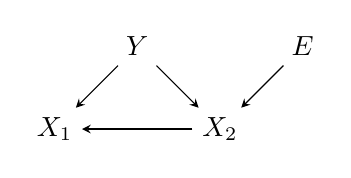
\begin{tikzpicture}[>=stealth, scale=1.05]
    \node (Y) at (0,1) {$Y$};
    \node (E) at (2,1) {$E$};
    \node (X1) at (-1,0) {$X_1$};
    \node (X2) at (1, 0) {$X_2$};
    
    \draw[->] (E) -- (X2);
    \draw[->] (Y) -- (X2);
    \draw[->] (Y) -- (X1);
    \draw[->] (X2) -- (X1);
\end{tikzpicture}
% \end{minipage}\\[6pt]
% where $\oplus$ is addition mod $2$, and $h$ is an arbitrary function allowing each $e \in \Env$ to intervene on $X_2$. 

% Here, $\SB(Y) = \varnothing$, and the associated DAG violates Asm.~\ref{as:A2}. There exists a classifier $f\colon \mathcal{X} \to [0,1]$ achieving uniformly lower Brier score risk than $f_{\SB(Y)} \equiv 1/2$: for all $e \in \Env$,
% $$R_e(f) \leq p(1-p) < \tfrac{1}{4} = R_e(f_{\SB(Y)}).$$
% \end{example}

% In this example, taking $X_2 \not\in \SB(Y)$ into account allows a classifier to adapt to the noise level in $X_1$. See \Cref{app:cont_example} for a regression variant of this example \linus{[TODO]}. 


% Ex.~\ref{ex:star_counterexample} is not an isolated case in the following sense: \eqref{eq:star} is necessary in that for any DAG in which it fails, there exists an SCM for which $f_{\SB(Y)}$ is not worst-case optimal. \jonas{[now, there is a discrepancy, as the above example is classification and the proposition is regression?]} \linus{[I think one can generalize the construction in the proof to also $Y \in \{0,1\}$, but then some parts of the proof would have to be rewritten. I suggest I try this later, in case there is enough time.]}

% \begin{proposition}
 
% Assume $\mathcal Y=\mathbb R$.
% Let $\G$ be a DAG over $(X_1,\ldots,X_d,Y,E)$ with $E$ a source node,
% no edge $E\to Y$, and let $\G_0$ be the induced subgraph on
% $(X_1,\ldots,X_d,Y)$. If \eqref{eq:star} fails, then there exists a
% set of environment $\Env$ and an SCM with graph $\G$ and induced distribution $\P$ such that
% (i) there exists $e_0\in\Env$ under which $\P_{e_0}$ is
% faithful w.r.t.\ $\G_0$,
% (ii) the second part of Asm.~\ref{as:A2} holds \felix{[make this more precise. What is the second part]} \linus{(that is, for all $e \in \Env$ there exists an environment $e' \in \Env$ for which every $j \in \CH_\mathrm{int}(Y)$ is set independently of all other variables, with all other structural assignments unchanged)}, and
% (iii) there exists a measurable $f\colon\mathcal X\to\mathbb R$ with
% $R_e(f)<R_e(f_{\SB(Y)})$ for all $e\in\Env$.
% \end{proposition}
% % \begin{proposition}
% %  
% % Assume $\mathcal Y=\mathbb R$ and $\ell(y,q)=(y-q)^2$.
% % Let $\G$ be a DAG over $(X_1,\ldots,X_d,Y,E)$ with $E$ a source node,
% % no edge $E\to Y$, and suppose \eqref{eq:star} fails.
% % Then there exists an SCM with graph $\G$, whose induced
% % distribution is Markov with respect to $\G$, such that the intervention
% % part of Asm.~\ref{as:A2} holds, and there exists a measurable
% % $f\colon\mathcal X\to\mathbb R$ such that for all $e \in \Env$,
% % \[
% % R_e(f)<R_e\bigl(f_{\SB(Y)}\bigr).
% % \]
% % \end{proposition}
% % \begin{proposition}  
% % Let $\G$ be a DAG over $(X_1, \ldots, X_d, Y, E)$ with $E$ a source node, no edge $E \to Y$, and suppose \eqref{eq:star} fails. Then there exists an SCM with induced distribution $\P$ that is Markov and faithful w.r.t.\ $\G$ and a measurable $f\colon \mathcal{X} \to \mathcal{A}$ such that for all $e \in \Env$, $R_e(f) < R_e(f_{\SB(Y)}).$
% % \end{proposition}

% %\rml{Together, Ex.~\ref{ex:star_counterexample} and \Cref{prop:star_necessary} show that \eqref{eq:star} determines at the graph level whether worst-case optimality of $f_{\SB(Y)}$ can hold under suitable environments.}

% \subsection{Additional intervention targets}
% \jonas{[new results -- Linus has written down the  proof I think?]}

% \subsection{Worst-case optimal functions} 

% So far, we have studied predictors $f_S(x) = \E[Y \given X_S = x_S]$ defined by an invariant subset $S$ (the `subset view'). \Cref{thm:worst_case} shows that, under Asm.~\ref{as:A1} or~\ref{as:A2}, $f_{\SB(Y)}$ is worst-case optimal over all measurable functions $f\colon \mathcal{X} \to \mathcal{A}$ (the `function view'). We now outline three reasons why the subset view is the right choice in our setting: function-view methods can use a weaker notion of invariance than the subset view, functions satisfying strong invariance criteria can still have strictly larger worst-case risk than $f_{\SB(Y)}$, and the subset view is more interpretable.

% To solve Problem~\eqref{eq:worst-case}, Invariant Risk Minimization (IRM) \citep{arjovskyInvariantRiskMinimization2020} takes a function view and jointly learns a representation $\Phi\colon \mathcal{X} \to \mathcal{H}$ and a predictor $w\colon \mathcal{H} \to \mathcal{A}$. The representation $\Phi$ is required to be invariant in the sense that the optimal predictor $w$ on top of $\Phi$ is the same across environments. While failure cases of IRM are known \citep{rosenfeldRisksInvariantRisk2021, kamathDoesInvariantRisk2021}, we use the $0$--$1$ loss in the following example to make the point that IRM's invariance criterion can be weaker than the conditional invariance $Y \indep E \given X_S$ of Definition~\ref{def:inv_subset}.

% \linus{[Further drawback of IRM: unclear w.r.t. which kinds of shift this is invariant; see also \citep{subbaswamyUnifyingCausalFramework2022}, Sec 7]}

% \begin{example}[Weak IRM invariance under $0$--$1$ loss]  
% Consider the following SCM\\[0pt]
% \begin{minipage}{0.49\textwidth}
% \begin{align*}
%     X_1 &\coloneq \bm{1}\{\varepsilon_1 \leq E/10\}, \\
%     Y &\coloneq \bm{1}\{\varepsilon_Y \leq 1/4 + X_1/2\}, \\
%     X_2 &\coloneq Y \oplus \bm{1}\{\varepsilon_2 \leq E/10\},
% \end{align*}
% \end{minipage}
% \begin{minipage}{0.49\textwidth}
% \centering
% \vspace*{0.7em}
% 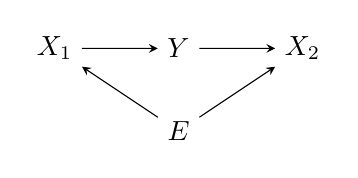
\begin{tikzpicture}[>=stealth, scale=1.05]
    \node (X1) at (-1.5,1) {$X_1$};
    \node (Y) at (0,1) {$Y$};
    \node (X2) at (1.5,1) {$X_2$};
    \node (E) at (0,0) {$E$};

    \draw[->] (X1) -- (Y);
    \draw[->] (Y) -- (X2);
    \draw[->] (E) -- (X1);
    \draw[->] (E) -- (X2);
\end{tikzpicture}
% \end{minipage}\\[6pt]
% where $\varepsilon_1, \varepsilon_Y, \varepsilon_2 \sim \mathrm{Unif}([0,1])$, mutually independent, and $\oplus$ denotes addition modulo $2$. Set $\Envtr = \{1, 2, 3\}$ and $\Env = \Envtr \cup \{8\}$.

% Subset methods: only $S = \{1\}$ is invariant, with $\P_e(Y^e = 1 \given X_1^e = 1) = 3/4$ and $\P_e(Y^e = 1 \given X_1^e = 0) = 1/4$ for all $e \in \Env$. The classifier $f_{\{1\}}$ achieves $3/4$ accuracy in every environment.

% IRM: consider the representation $\Phi(x) \coloneq x_2$. Although $\P_e(Y = 1 \given X_2 = 1)$ varies across $\Envtr$, it stays above $1/2$ in every training environment, so the classifier $w = \mathrm{id}$ is Bayes-optimal under the $0$--$1$ loss in all $e \in \Envtr$.
% % and $\Phi$ satisfies the IRM invariance criterion
% The resulting accuracy ranges from $9/10$ to $7/10$ across $\Envtr$, exceeding the $3/4$ of $f_{\{1\}}$ on average. In the test environment $e = 8$, the accuracy of $w \circ \Phi$ drops to $1/5$.
% %A subset method detects the non-invariance of $\{2\}$ from training data, while IRM uses the spurious representation because its invariance criterion does not capture the variation.
% \end{example}

% In Ex.~\ref{ex:irm-vs-subset}, IRM accepts $\Phi$ as invariant because the Bayes-optimal classifier under $0$--$1$ loss does not change across $\Envtr$, although $Y \notindep E \given \Phi(X)$. Under a loss strictly consistent for the mean functional, IRM would reject $\Phi$. The example nevertheless makes the point that function-based invariance criteria can be weaker than the conditional invariance used in the subset view.

% Next, we provide an example where a function satisfies significantly stronger invariances, however, its worst-case risk exceeds that of $f_{\SB(Y)}$. We illustrate that the flexibility of the function view can have a downside: a function has more potential to exploit a pattern on $\Envtr$ that does not persist on $\Env$.

% \begin{example}[Worst-case suboptimality of an invariant $f$]  
% Let $\mathcal{Y} = \mathbb{R}$, $\ell(y,q) = (y-q)^2$, and consider the following SCM over $(X_1, X_2, Y, E)$ whose structural assignments on $\Envtr$ are\\[0pt]
% \begin{minipage}{0.49\textwidth}
% \begin{align*}
%     Y &\coloneq \varepsilon_Y, \\
%     X_1 &\coloneq \delta_E + Y + \varepsilon_1, \\
%     X_2 &\coloneq \delta_E + \varepsilon_2, \\
%     \text{where }& \delta_E \in \mathbb{R} \text{ and } \varepsilon_Y, \varepsilon_1, \varepsilon_2 \stackrel{\text{i.i.d.}}{\sim} \mathcal{N}(0,1).
% \end{align*}
% \end{minipage}
% \begin{minipage}{0.49\textwidth}
% \centering
% \vspace*{1.5em}
% 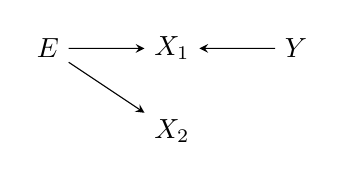
\begin{tikzpicture}[>=stealth, scale=1.05]
    \node (E) at (-1.5,1) {$E$};
    \node (X1) at (0,1) {$X_1$};
    \node (Y) at (1.5,1) {$Y$};
    \node (X2) at (0,0) {$X_2$};

    \draw[->] (E) -- (X1);
    \draw[->] (E) -- (X2);
    \draw[->] (Y) -- (X1);
\end{tikzpicture}
% \end{minipage}\\[6pt]
% Here, $\SB(Y) = \varnothing$, so $f_{\SB(Y)} = \E[Y] = 0$. The representation $\Phi(X) \coloneq X_1-X_2 = Y + \varepsilon_1 - \varepsilon_2$ is independent of $E$ on $\Envtr$, and the predictor $f(x) \coloneq \E[Y \given \Phi = x_1-x_2] = (x_1-x_2)/3$ is optimal for the squared loss on top of $\Phi$. For all $e \in \Envtr$, $R_e(f) = \frac{2}{3}< 1 = R_e(f_{\SB(Y)})$.
% % \begin{equation}  
% %     R_e(f) = \E_e[(Y - f(X))^2]= \Var(Y \given \Phi) = 1 - \frac{\Cov(Y, \Phi)^2}{\Var(\Phi)} = \frac{2}{3}< 1 = R_e(f_{\SB(Y)}).
% % \end{equation}



% On $\Envtr$, $f$ satisfies several invariance properties: (i) $Y \indep E \given f(X)$, and thus $\E_e[Y \given \Phi(X)]$ does not depend on $e \in \Envtr$, so $\Phi$ satisfies the IRM invariance criterion of \citet[Definition~3]{arjovskyInvariantRiskMinimization2020}; (ii) $E \indep f(X)$; (iii) invariant residuals $Y - f(X) \indep E$, the invariance notion used by \citep{saengkyongamExploitingIndependentInstruments2022}; and (iv) invariance of the risks.

% We now extend the SCM to $\Env$: for all $e\in\Envtr$, let $\Env$ contain an environment $e'$ in which the structural assignment of $X_1$ is replaced by $X_1\coloneq\tilde\varepsilon_1\sim\mathcal{N}(0,1)$, independent of $(Y,\varepsilon_1,\varepsilon_2)$, while the assignments $X_2$ is unchanged. Then Asm.~\ref{as:A2} holds. In environment $e'$, $f(X)=(\tilde\varepsilon_1-\delta_e-\varepsilon_2)/3$ is independent of $Y$. Furthermore, 
% $R_{e'}(f) = 1 + (2 + \delta_e^2)/9 > 1 = R_{e'}(f_{\SB(Y)}), $
% and hence, $\sup_{e \in \Env}R_e(f) > \sup_{e\in\Env} R_e(f_{\SB(Y)})$, that is, Inequality~\eqref{eq:worst_case_statement} is strict. 
% \end{example}

% In Ex.~\ref{ex:strict-inequality}, $f$ exploits a pattern on $\Envtr$ that does not extend to $\Env$. Our setup in \Cref{sec:chamber_experiments} makes few structural assumptions on the interventions, and in this regime the subset view is the safer choice. \Cref{thm:worst_case} formalizes this. If the interventions are restricted to a known class, the function view can instead be preferable: anchor regression \citep{rothenhauslerAnchorRegressionHeterogeneous2020}, for instance, is worst-case optimal over a specific class of bounded shift interventions. We focus on the more general case.

% The subset view is also more interpretable and transparent: it combines feature selection with standard supervised learning, rather than an opaque function of all covariates. In regulated settings such as credit scoring or clinical decision support, this simplifies auditing and certifying that prohibited features are not used, and makes individual predictions easier to explain. Only the variables in the chosen invariant subset $S \subseteq \{1, \ldots, d\}$ need to be measured at deployment. The choice of inputs also influences the behavior of agents interacting with the model, as in the lending example of \Cref{sec:intro}: using causal features such as income encourages applicants to improve their actual creditworthiness, whereas using manipulable downstream variables invites gaming.



% \subsubsection[placeholder -- ignore for the structure]{Extension to changing intervention targets}

% \linus{[With our new setup, we could structure section 4 maybe as follows:]}
% \begin{itemize}
%     \item Problem~\eqref{eq:pred_intervention_game} is hard: the follower picks $e$ from $\EnvC{A}$ according to a criterion that need not be aligned with the loss $\ell$, and the set $\Env^*(f)$ over which we take the worst case depends on the predictor through $R^{\mathrm{ad}}$. We proceed by upper bounding our stackelberg risk by the worst-case risk over the entire set $\EnvC{A}$,
%     \begin{equation} \label{eq:upper_bound}
%         \sup_{e \in \Env^*(f)} R_e(f)
%         \leq
%         \sup_{e \in \EnvC{A}} R_e(f),
%     \end{equation}
%     and minimizing the right-hand side. When $\ell^{\mathrm{ad}} = \ell$, the two sides of~\eqref{eq:upper_bound} coincide, and the right-hand side is the worst-case risk in the classical distributional-generalization sense.

%     \item This section establishes three results. First, $f_{\SB(Y)}$ minimizes the right-hand side of~\eqref{eq:upper_bound} among all $\sigma(X_{\DEYforb^C})$-measurable predictors (Theorem~XYZ), and it does so uniformly in $e$. As a direct consequence, $f_{\SB(Y)}$ dominates $f_{\PA(Y)}$ in every environment, and hence also in Problem~\eqref{eq:pred_intervention_game} itself (Corollary~XYZ). Second, under additional assumptions on the training environments, the stable blanket is worst-case optimal over $\EnvC{A}$ among all measurable predictors (Theorem~XYZ). Third, without these assumptions, the stable blanket is not always optimal (Section~XYZ).
    
%     \item The environments in $\EnvC{A}$ extend the training-time environments by allowing the follower to change the structural assignments of $X_{\CH(E)}$ using additional parents from a set $A \subseteq \{1, \ldots, d\}$. We assume throughout this section that $A \subseteq \DEYforb^C \setminus \{Y, E\}$ (such that $\Gplus$ is acyclic; multiple choices possible). \linus{[Argue why this is reasonable, and that the follower would not introduce cycles]}. Let $\Gplus$ be the DAG obtained from $\G$ by adding all edges $k \to j$ with $j \in \CH_{\G}(E)$ and $k \in A$ such that $\Gplus$ is acyclic. Then, the stable blanket in $\G$ is the same as the stable blanket in $\Gplus$:
%         \begin{lemma}[Stable blanket under graph augmentation] %\label{lem:augmentation}
%         Assume that $A \subseteq \DEYforb^C \setminus \{Y, E\}$. Then, the augmented DAG $\Gplus$ satisfies $\DEforbg{\Gplus} = \DEforbg{\G}$ and $\SBg{\Gplus} = \SBg{\G}$. In particular, $Y \dsep{\Gplus} E \given \SBg{\G}$.
%         \end{lemma}
%     Proof in \Cref{app:proof_augmentation}. Consequently, $\SBg{\Gplus}$ is in theory identifiable already from the training-time environments.

%     \item \begin{theorem}[Uniform optimality of $\SB(Y)$] \label{thm:pointwise_worst_case}
%     For all $\sigma(X_{\DEYforb^C})$-measurable $f\colon \mathcal{X} \to \mathcal{A}$ and all $e \in \EnvC{A}$,
%     \begin{equation} %\label{eq:pointwise_statement}
%         R_e(f) \geq R_e(f_{\SB(Y)}).
%     \end{equation}
%     \end{theorem}

%     \item The uniform optimality in $e$ gives a direct comparison of the stable blanket and the causal parents in Problem~\eqref{eq:pred_intervention_game}.
%     \begin{corollary}[Parents vs.\ stable blanket] %\label{cor:PA_vs_SB}
%     For all $e \in \EnvC{A}$, $R_e(f_{\PA(Y)}) \geq R_e(f_{\SB(Y)})$. Consequently, 
%     \begin{equation} %\label{eq:PA_vs_SB_adversarial}
%         \sup_{e \in \Env^*(f_{\SB(Y)})} R_e(f_{\SB(Y)})
%         \leq
%         \sup_{e \in \Env^*(f_{\SB(Y)})} R_e(f_{\PA(Y)}).
%     \end{equation}
%     \end{corollary}
%     \item Then: rest of section 3 with $\Env = \EnvC{A}$. Potentially include: example where SB changes in different environments because follower adds/deletes edges (if we use a different $A$ than we assume)

% \end{itemize}




% {
% \color{mygreen}

% Unlike these works, we focus on selecting an invariant subset of covariates
% for prediction, a topic studied in causal
% inference~\citep{rojas-carullaInvariantModelsCausal2018, christiansenCausalFrameworkDistribution2021}.
% We connect prediction-intervention games to causal distribution
% generalization, building on the stable blanket
% of~\citet{pfisterStabilizingVariableSelection2021} to strengthen related
% worst-case results.
% We further allow follower interventions that modify the SCM, going beyond
% the fixed-graph setting common in causal strategic classification and
% distribution generalization work.
% To our knowledge, prediction-intervention games are new, as is our
% worst-case analysis of stable-blanket predictors via distribution
% generalization, for general response variables and follower objectives.
% \Cref{app:extended_related_works} gives a more complete discussion.

% Unlike these works, we focus on selecting an invariant subset of covariates
% for prediction, a topic studied in causal inference. We further allow the
% follower to modify the SCM, in contrast to the fixed-graph setting of most
% causal Stackelberg and distribution generalization work.
% We connect prediction-intervention games to causal distribution
% generalization~\citep{rojas-carullaInvariantModelsCausal2018, christiansenCausalFrameworkDistribution2021};
% in particular, we use the stable blanket
% of~\citet{pfisterStabilizingVariableSelection2021} and strengthen related
% worst-case results.
% To our knowledge, for general response variables and follower objectives,
% the combination of follower interventions that modify the SCM and
% worst-case analysis of stable-blanket predictors is new.
% \Cref{app:extended_related_works} gives a more complete discussion.




% }



% {
% \color{orange}
% Unlike these works, we focus on prediction based on invariant subsets of
% covariates, a topic studied in causality through invariant prediction and
% distribution generalization
% \citep{rojas-carullaInvariantModelsCausal2018, christiansenCausalFrameworkDistribution2021}.
% We connect prediction-intervention games to this literature; in particular,
% our worst-case analysis builds on the stable blanket of
% \citet{pfisterStabilizingVariableSelection2021} and strengthens related
% worst-case results.
% We also allow follower interventions that modify the SCM, going beyond the
% fixed-graph setting common in causal strategic classification and distribution
% generalization.
% \Cref{app:extended_related_works} gives a more complete discussion.

% Compared with this literature, we explicitly study how different invariant
% subsets of covariates perform in the resulting game. We connect
% prediction-intervention games to invariant prediction and distribution
% generalization
% \citep{rojas-carullaInvariantModelsCausal2018,
% christiansenCausalFrameworkDistribution2021}; in particular, our worst-case
% analysis builds on the stable blanket of
% \citet{pfisterStabilizingVariableSelection2021} and strengthens related
% worst-case results. We also allow follower interventions that add edges to the
% DAG, whereas most related settings keep the graph fixed. To our knowledge,
% worst-case analysis of stable-blanket predictors in such
% follower-intervention games has not been studied before.
% \Cref{app:extended_related_works} gives a more complete discussion.

% We allow for binary and continuous responses, follower objectives that differ
% from the leader's loss, and interventions constrained by an SCM. This connects
% prediction-intervention games to invariant prediction and distribution
% generalization, where predictors based on invariant covariate sets have been
% studied in causality
% \citep{rojas-carullaInvariantModelsCausal2018,
% christiansenCausalFrameworkDistribution2021}. In particular, our worst-case
% analysis builds on the stable blanket of
% \citet{pfisterStabilizingVariableSelection2021} and strengthens related
% worst-case results. We also allow follower interventions to add edges to the
% DAG, whereas most related settings keep the graph fixed. To our knowledge,
% the combination of SCM-constrained follower interventions, follower objectives
% distinct from the leader's loss, and worst-case analysis of stable-blanket
% predictors is new. \Cref{app:extended_related_works} gives a more
% complete discussion.
% }